%# -*- coding: utf-8 -*-
%!TEX encoding = UTF-8 Unicode
%!TEX TS-program = xelatex
%~ \XeTeXinputencoding "UTF-8"
% vim:ts=4:sw=4
%
% 以上设定默认使用 XeLaTex 编译,并指定 Unicode 编码,供 TeXShop 自动识别

% Author: Yunhui Fu <yhfudev@gmail.com>
% License: Creative Commons (CC BY 4.0)

\documentclass[letter,12pt,onecolumn]{article}
%\documentclass[letter,12pt,onecolumn]{book}

\newcommand{\doctitle}{\cnt{UFLDL Tutorial}{UFLDL教程}{}}
\newcommand{\docauthor}{ver 201406}
\newcommand{\dockeywords}{}
\newcommand{\docsubject}{}

\newcommand{\docversion}[0]{2014-06-11}

\newcommand{\usedefaultTWO}[2]{
\if\relax\detokenize{#2}\relax
  #1
\else
  #2
\fi
}

\newcommand{\usedefaultTHREE}[3]{
\if\relax\detokenize{#3}\relax
  \usedefaultTWO{#1}{#2}
\else
  #3
\fi
}

% 用于接受从 xelatex/pdflatex 通过参数 -jobname 传入的参数来判定编译何种语言的版本。
% \cnt 的三个参数分别为 en/zh/tw 的内容
\newcommand{\cnt}[3]{{#1}{#2}{#3}}
%\newcommand{\cnt}[3]{#1} % default en
\usepackage{ifthen}
\ifthenelse{\equal{\detokenize{lang-zh}}{\jobname}}{
  \renewcommand{\cnt}[3]{\usedefaultTWO{#1}{#2}}
}{
  \ifthenelse{\equal{\detokenize{lang-tw}}{\jobname}}{
    \renewcommand{\cnt}[3]{\usedefaultTHREE{#1}{#2}{#3}}
  }{
    % default en
    \renewcommand{\cnt}[3]{#1}
    %\renewcommand{\cnt}[3]{#2}
  }
}

\newcommand{\cnts}[3]{{#1} {#2}}

% 根据配置来设置中文环境
\newcommand\charsetzhcn[1]{#1} % the charset encoding for zh_CN
\newcommand\formatzhcn[1]{#1} % the page format for zh_CN
\cnt{
\renewcommand\charsetzhcn[1]{} % the charset encoding for zh_CN
\renewcommand\formatzhcn[1]{} % the page format for zh_CN
}{
\renewcommand\charsetzhcn[1]{#1} % the charset encoding for zh_CN
\renewcommand\formatzhcn[1]{#1} % the page format for zh_CN
}{
\renewcommand\charsetzhcn[1]{#1} % the charset encoding for zh_CN
\renewcommand\formatzhcn[1]{#1} % the page format for zh_CN
}

%# -*- coding: utf-8 -*-
%!TEX encoding = UTF-8 Unicode
%!TEX TS-program = xelatex
% vim:ts=4:sw=4
%
% 以上设定默认使用 XeLaTex 编译,并指定 Unicode 编码,供 TeXShop 自动识别

% 使用 LaTex 写中文的配置模板
%\documentclass[12pt]{article}

%\newcommand{\doctitle}{Peer-to-Peer Communication Across Network Address Translators}
%\newcommand{\doctitle}{穿越NAT的点对点通信}
%\newcommand{\docauthor}{Bryan Ford \& Pyda Srisuresh \& Dan Kegel}
%\newcommand{\dockeywords}{NAT穿越, 点对点, NAT Traversal, Peer-to-Peer}
%\newcommand{\docsubject}{NAT穿越}
%\newcommand\charsetzhcn[1]{#1} % the charset encoding for zh_CN
%\newcommand\formatzhcn[1]{#1} % the page format for zh_CN

\newcommand\mymainfont{Times New Roman}
\newcommand\mymonofont{FreeMono}%{AR PL UMing CN}%{FreeMono} %{WenQuanYi Micro Hei Mono} %{Monaco}
\newcommand\myboldfont{WenQuanYi Micro Hei Mono}%{AR PL UKai CN}%{YaHei Consolas Hybrid}%{黑体}%{標楷體}
\newcommand\mysansfont{FreeSans}
\newcommand\myitalicfont{Times New Roman} %{Garamond}

\newcommand\mycjkboldfont{WenQuanYi Micro Hei Mono}%{Adobe Heiti Std}%{AR PL UKai CN}%{YaHei Consolas Hybrid}%{黑体}%{標楷體}
\newcommand\mycjkitalicfont{Adobe Kaiti Std}
\newcommand\mycjkmainfont{AR PL UMing CN}%{Adobe Song Std}%{仿宋}%{宋体}%{新宋体}%{文鼎PL新宋}%
\newcommand\mycjksansfont{Adobe Ming Std}
\newcommand\mycjkmonofont{WenQuanYi Micro Hei Mono}%{AR PL UMing CN}%{WenQuanYi Micro Hei Mono}

\usepackage{ifthen}
\usepackage{ifpdf}
\usepackage{ifxetex}
\usepackage{ifluatex}

\usepackage{color}
\usepackage[rgb]{xcolor}


\usepackage[cm-default]{fontspec} % XeLaTex 配合 fontspec

\charsetzhcn{
  %\renewcommand\mycjkmainfont{AR PL UMing CN}%{仿宋}%{宋體}%{新宋體}%{文鼎PL新宋}%

  \ifxetex    % xelatex

    %\usepackage[cm-default]{fontspec} % XeLaTex 配合 fontspec 可以非常方便地设置字体。[cm-default]选项主要用来解决使用数学环境时数学符号不能正常显示的问题
    %\usepackage{xltxtra,xunicode} %这行和上行 \usepackage[cm-default]{fontspec} 解决公式不正常的问题.但是打开后有些如 itemize 的点不能显示。

    \usepackage[
        BoldFont, % 允許粗體
        SlantFont,        % 允許斜體
        %CJKsetspaces,
        CJKchecksingle
        ]{xeCJK}
    \defaultfontfeatures{Mapping=tex-text} %如果沒有它,會有一些 tex 特殊字符無法正常使用,比如連字符。

    \XeTeXlinebreaklocale "zh"                      % 重要,使得中文可以正確斷行!
    \XeTeXlinebreakskip = 0pt plus 1pt minus 0.1pt  %

    \setCJKmainfont[BoldFont=\mycjkboldfont, ItalicFont=\mycjkboldfont]{\mycjkmainfont}
    \setCJKsansfont{\mycjksansfont}%{Adobe Ming Std} %{AR PL UMing CN} %{Microsoft YaHei}
    \setCJKmonofont{\mycjkmonofont}

  \fi


\formatzhcn{
    %\newfontfamily{\j}{Osaka}       % 设置特殊字符,这里是为日文准备的特殊字体。没有该字体,所以关闭。

    \setlength{\parindent}{2.04em}  %设置首行缩进。只有中文才打开。
    \linespread{1.3}                % 设置行距

    %\definecolor{bisque}{rgb}{.996,.891,.755}
    %\pagecolor{bisque} % 设置背景颜色

    % 设置原文照排环境的字体
    \makeatletter
    \def\verbatim@font{\sffamily\small}
    \makeatother

    % 将默认的英文重定义为中文
    \renewcommand{\contentsname}{\cnt{Content}{目录}{目錄}}
    \renewcommand{\listfigurename}{\cnt{List of Figures}{插图目录}{插圖目錄}}
    \renewcommand{\listtablename}{\cnt{List of Tables}{表格目录}{表格目錄}}
    \renewcommand{\indexname}{\cnt{Index}{索引}{索引}}
    \renewcommand{\tablename}{\cnt{Table}{表}{表}}
    \renewcommand{\figurename}{\cnt{Figure}{图}{圖}}
    \renewcommand{\appendixname}{\cnt{Chapter}{附录}{附錄}}

    % article
    %\renewcommand{\refname}{\cnt{Bibliography}{参考文献}{參考文獻}}
    %\renewcommand{\abstractname}{\cnt{Abstract}{摘要}{摘要}}

    % book
    %\renewcommand{\chaptername}{\cnt{Chapter}{章节}{章節}}
    %\renewcommand{\bibname}{\cnt{Bibliography}{参考}{參考}}

    %\renewcommand{\IEEEkeywordsname}{\cnt{Keywords}{关键词}{關鍵詞}}


    % 设置页眉页脚
    \usepackage[pagestyles,compact]{titlesec} % 定制页眉页脚
    \newpagestyle{main}{%
        \sethead[$\cdot$~\thepage~$\cdot$][][\thesection\quad%
        \sectiontitle]{\thesection\quad\sectiontitle}{}{%
            $\cdot$~\thepage~$\cdot$}
        \setfoot{}{}{}\headrule}
        \pagestyle{main}
        \renewpagestyle{plain}{\sethead{}{}{}\setfoot{}{}{}}
    \pagestyle{plain}

    %% 设置chapter, section与subsection的格式
    \titleformat{\chapter}{\centering\huge}{\textbf{第\thechapter{}章}}{1em}{\textbf}
    \titleformat{\section}{\centering\LARGE}{\textbf{\thesection}}{1em}{\textbf}
    \titleformat{\subsection}{\Large}{\textbf{\thesubsection}}{1em}{\textbf}

    %% For LaN
    \newcommand{\LaN}{L{\scriptsize\hspace{-0.47em}\raisebox{0.23em}{A}}\hspace{-0.1em}N}

    %% 去掉表头中的冒号
    \makeatletter
        \long\def\@makecaption#1#2{%
            \vskip\abovecaptionskip
            \sbox\@tempboxa{#1~~#2}%
            \ifdim \wd\@tempboxa >\hsize
                #1~~#2\par
            \else
                \global \@minipagefalse
                \hb@xt@\hsize{\hfil\box\@tempboxa\hfil}%
            \fi
            \vskip\belowcaptionskip}
    \makeatother
} % formatzhcn

} % \charsetzhcn

%\setmainfont{\mymainfont}        % 英文衬线字体, setmainfont=setromanfont
\setromanfont[Mapping=tex-text,  % 沿用 LaTex 的一些习惯的标点转换,例如 en-dash 以两个减号表示
    Ligatures={Required,Common}, % 如果此字体内置 Ligatures 定义则启用
    ItalicFont={\myitalicfont},  % 斜体用 Times Italic,严格来说只有拉丁子母有斜体。
    BoldFont={\myboldfont}]      % 粗体用字体
    {\mymainfont}                % 内文使用字体, Linux 下用 "fc-list :lang=zh-cn" 列出支持的中文字体
\setmonofont[Scale=0.8]{\mymonofont} % 英文等宽字体
\setsansfont{\mysansfont}       % 英文无衬线字体

% 设置中文状态下, 恢复 lstlisting 的 mono 字体
\usepackage[T1]{fontenc}
\DeclareTextCommandDefault{\nobreakspace}{\leavevmode\nobreak\ } % EU1 encoding setup has changed \nobreakspace from being an encoding-independent command to an encoding-dependent command, but without setting up a default definition so it works in all encodings.

\usepackage{dtklogos} % \LaTeXe 等
% XeTeX logo
%\def\XeTeX{\leavevmode
%    \setbox0=\hbox{X\lower.5ex\hbox{\kern-.15em\reflectbox{E}}\kern-.1667em \TeX}%
%    \dp0=0pt\ht0=0pt\box0}

% the algorithm2e package
\makeatletter
\newif\if@restonecol
\makeatother
\let\algorithm\relax
\let\endalgorithm\relax
\usepackage[ruled,vlined]{algorithm2e} %\usepackage[figure,ruled,vlined]{algorithm2e}

\usepackage{url}
\usepackage{array}

\usepackage{courier}
\usepackage{listings} % list the source code
\definecolor{ForestGreen}{rgb}{0.13,0.55,0.13}

\lstset{
    language=C,
    captionpos=b, %t,
    tabsize=3,
    basicstyle=\footnotesize\ttfamily, %basicstyle=\ttfamily\normalsize, %basicstyle=\small\ttfamily, %\normalfont\ttfamily, % \large\ttfamily, % \small\ttfamily, % \footnotesize\ttfamily, % \scriptsize\ttfamily, % Standardschrift,
    numbers=left,               %左侧显示行号 往左靠,还可以为right,或none,即不加行号
    stepnumber=1,               %若设置为2,则显示行号为1,3,5,即stepnumber为公差,默认stepnumber=1
    %numberstyle=\tiny,         %行号字体用小号
    numberstyle={\color[RGB]{0,192,192}\tiny} ,%设置行号的大小,大小有tiny,scriptsize,footnotesize,small,normalsize,large等
    numbersep=8pt,              %设置行号与代码的距离,默认是5pt
    breaklines=true,            %对过长的代码自动换行
    showstringspaces=false,     %不显示代码字符串中间的空格标记
    frame=shadowbox, %=lines,                    %把代码用带有阴影的框圈起来
    stringstyle=\ttfamily,      % 代码字符串的特殊格式
    commentstyle=\color{ForestGreen}, %\color{red!50!green!50!blue!50}, %浅灰色的注释
    rulesepcolor=\color{red!20!green!20!blue!20}, %代码块边框为淡青色
    keywordstyle=\color{blue!90}\bfseries,        %代码关键字的颜色为蓝色,粗体
    backgroundcolor=\color[RGB]{245,245,244},   %代码背景色 \color[rgb]{0.91,0.91,0.91}
    framextopmargin=2pt,framexbottommargin=2pt,abovecaptionskip=-3pt,belowcaptionskip=3pt,
%    xleftmargin=4em,xrightmargin=4em, % 设定listing左右的空白
%    %language={[ISO]C++},       %language为,还有{[Visual]C++}
%    alsolanguage=Java,
%    %alsolanguage=[ANSI]C,      %可以添加很多个alsolanguage,如alsolanguage=matlab,alsolanguage=VHDL等
%    %alsolanguage= tcl,
%    alsolanguage= XML,
%    keepspaces=true,            %
%    breakindent=22pt,           %
%    breakindent=4em,            %
%    showspaces=false,           %
%    flexiblecolumns=true,       %
%    breakautoindent=true,       %
%    aboveskip=1em,              %代码块边框
%    %% added by http://bbs.ctex.org/viewthread.php?tid=53451
%    fontadjust,
%    texcl=true,
%    escapeinside=``,            %在``里显示中文
%    %escapebegin=\begin{CJK*}{GBK}{hei},escapeend=\end{CJK*},
%    % 设定中文冲突,断行,列模式,数学环境输入,listing数字的样式
%    extendedchars=false,columns=flexible,
%    mathescape=false,
%    % numbersep=-1em,
    emph={label}
}

\renewcommand{\ttdefault}{pcr}

\definecolor{darkgreen}{cmyk}{0.7, 0, 1, 0.5}
\definecolor{darkblue}{rgb}{0.1, 0.1, 0.5}
\lstdefinelanguage{diff}
{
    keywords={+, -, \ , @@, diff, index, new},
    sensitive=false,
    morecomment=[l][""]{\ },
    morecomment=[l][\color{darkgreen}]{+},
    morecomment=[l][\color{red}]{-},
    morecomment=[l][\color{darkblue}]{@@},
    morecomment=[l][\color{darkblue}]{diff},
    morecomment=[l][\color{darkblue}]{index},
    morecomment=[l][\color{darkblue}]{new},
    morecomment=[l][\color{darkblue}]{similarity},
    morecomment=[l][\color{darkblue}]{rename},
}

\lstdefinelanguage{JavaScript}{
  keywords={typeof, new, true, false, catch, function, return, null, catch, switch, var, if, in, while, do, else, case, break},
  keywordstyle=\color{blue}\bfseries,
  ndkeywords={class, export, boolean, throw, implements, import, this},
  ndkeywordstyle=\color{darkgray}\bfseries,
  identifierstyle=\color{black},
  sensitive=false,
  comment=[l]{//},
  morecomment=[s]{/*}{*/},
  %commentstyle=\color{purple}\ttfamily,
  commentstyle=\color{green}\ttfamily,
  stringstyle=\color{red}\ttfamily,
  morestring=[b]',
  morestring=[b]"
}

\usepackage{tabularx} % long table
\usepackage{booktabs,longtable} % table in seperate pages.


\ifxetex % xelatex
\else
    %The cmap package is intended to make the PDF files generated by pdflatex "searchable and copyable" in acrobat reader and other compliant PDF viewers.
    \usepackage{cmap}%
\fi
% ============================================
% Check for PDFLaTeX/LaTeX
% ============================================
\newcommand{\outengine}{xetex}
\newif\ifpdf
\ifx\pdfoutput\undefined
  \pdffalse % we are not running PDFLaTeX
  \ifxetex
    \renewcommand{\outengine}{xetex}
  \else
    \renewcommand{\outengine}{dvipdfmx}
  \fi
\else
  \pdfoutput=1 % we are running PDFLaTeX
  \pdftrue
  \usepackage{thumbpdf}
  \renewcommand{\outengine}{pdftex}
  \pdfcompresslevel=9
\fi
\usepackage[\outengine,
    bookmarksnumbered, %dvipdfmx
    %% unicode, %% 不能有unicode选项,否则bookmark会是乱码
    colorlinks=true,
    citecolor=red,
    urlcolor=blue,        % \href{...}{...} external (URL)
    filecolor=red,      % \href{...} local file
    linkcolor=black, % \ref{...} and \pageref{...}
    breaklinks,
    pdftitle={\doctitle},
    pdfauthor={\docauthor},
    pdfsubject={\docsubject},
    pdfkeywords={\dockeywords},
    pdfproducer={Latex with hyperref},
    pdfcreator={pdflatex},
    %%pdfadjustspacing=1,
    pdfborder=1,
    pdfpagemode=UseNone,
    pagebackref,
    bookmarksopen=true]{hyperref}

% --------------------------------------------
% Load graphicx package with pdf if needed 
% --------------------------------------------
\ifxetex    % xelatex
    \usepackage{graphicx}
\else
    \ifpdf
        \usepackage[pdftex]{graphicx}
        \pdfcompresslevel=9
    \else
        \usepackage{graphicx} % \usepackage[dvipdfm]{graphicx}
    \fi
\fi

%% \DeclareGraphicsRule{.jpg}{eps}{.bb}{}
%% \DeclareGraphicsRule{.png}{eps}{.bb}{}
\graphicspath{{./} {figures/}}
\usepackage{flafter} % 防止图形在文字前

%%%% 字体:
%Adobe Heiti Std 和 Adobe Song Std是砖头公司出的两款超pp的字体,有人把它们用在latex排版中,效果超级好。
%windows版在 Program Files/Adobe/Acrobat 8.0/Resource/CIDFont 下。

%sudo mkdir /usr/share/fonts/adobe
%sudo cp DIR2adobefonts/*.otf /usr/share/fonts/adobe
%sudo chmod 644 /usr/share/fonts/adobe/*.otf # 当前用户读写,当前组用户读写,其他用户只读

%cd /usr/share/fonts/adobe/
%sudo mkfontscale #(创建fonts.scale文件,控制字体旋转缩放)
%sudo mkfontdir #(创建fonts.dir文件,控制字体粗斜体产生)
%sudo fc-cache -fv # (建立字体缓存信息,也就是让系统认识认识)
%fc-list :lang=zh-cn # 看看装上没


%安装 LaTeX+XeTeX环境的过程, 你也使用Emacs来编辑TeX文件的话, 那么一定要安上AUCTeX这个扩展
%sudo apt-get install texlive texlive-latex-extra texlive-xetex lmodern # 首先是LaTeX与XeTeX的安装

%sudo apt-get install auctex

%安装好以后, 重点是配置.emacs文件, 因为AUCTeX本身是不支持通过xelatex编译的.
%;; AUCTeX
%(defun auctex ()
  %(add-to-list 'TeX-command-list '("XeLaTeX" "%`xelatex%(mode)%' %t; %`xelatex%(mode)%' %t" TeX-run-TeX nil t)) ;; 这里我编译了两次
    %(setq TeX-command-default "XeLaTeX") ;; 设定默认编译命令为XeLaTeX
    %(setq TeX-save-query nil)            ;; 保存之前不询问
    %(setq TeX-show-compilation t))       ;; 在新窗口显示编译过程
%(add-hook 'LaTeX-mode-hook 'auctex)

%(custom-set-variables
 %'(TeX-output-view-style (quote (("^dvi$nnnnnnn" ("^landscape$" "^pstricks$\\|^pst-\\|^psfrag$") "%(o?)dvips -t landscape %d -o && gv %f") ("^dvi$" "^pstricks$\\|^pst-\\|^psfrag$" "%(o?)dvips %d -o && gv %f") ("^dvi$" ("^a4\\(?:dutch\\|paper\\|wide\\)\\|sem-a4$" "^landscape$") "%(o?)xdvi %dS -paper a4r -s 0 %d") ("^dvi$" "^a4\\(?:dutch\\|paper\\|wide\\)\\|sem-a4$" "%(o?)xdvi %dS -paper a4 %d") ("^dvi$" ("^a5\\(?:comb\\|paper\\)$" "^landscape$") "%(o?)xdvi %dS -paper a5r -s 0 %d") ("^dvi$" "^a5\\(?:comb\\|paper\\)$" "%(o?)xdvi %dS -paper a5 %d") ("^dvi$" "^b5paper$" "%(o?)xdvi %dS -paper b5 %d") ("^dvi$" "^letterpaper$" "%(o?)xdvi %dS -paper us %d") ("^dvi$" "^legalpaper$" "%(o?)xdvi %dS -paper legal %d") ("^dvi$" "^executivepaper$" "%(o?)xdvi %dS -paper 7.25x10.5in %d") ("^dvi$" "." "%(o?)xdvi %dS %d") ("^pdf$" "." "acroread %o %(outpage)") ("^html?$" "." "netscape %o")))))

%最后那个有点长, 主要是没有找到合适的方法像添加XeLaTeX一样只需要写新增的条目, 所以这里就把原有的和修改以后的都写了出来. 其实只改了一个地方, 已经用蓝色标注出来了, 就是在使用C-c C-v预览PDF文件的时候使用什么软件来打开. 我这里就是acroread, 你用的其它的话, 可以相应修改.
%这样修改好以后, 以后就可以直接使用C-c C-c编译, C-c C-v预览, C-c `在错误间跳转了.

%但是TeX Live中的install-info文件会导致源安装AUCTeX的时候失败, 所以如果是先安装的TeX Live, 再安装AUCTeX, 就需要先把TeX Live的install-info"消灭"掉: 
%sudo mv /usr/local/bin/install-info /usr/local/bin/install-info.bak

%-------------------------------------------------------------------
%终于搞定在emacs+auctex中设置xelatex为默认编译命令!

%只要在在~/.emacs中加上

%(add-hook 'LaTeX-mode-hook (lambda()
    %(add-to-list 'TeX-command-list '("XeLaTeX" "%`xelatex%(mode)%' %t" TeX-run-TeX nil t))
    %(setq TeX-command-default "XeLaTeX")
    %(setq TeX-save-query  nil )
    %(setq TeX-show-compilation t)
    %))

%第一行参考auctex的手册auctex.pdf,版本是11.84 ;
%(add-to-list 'TeX-command-list '("XeLaTeX" "%`xelatex%(mode)%' %t" TeX-run-TeX nil t)) 会在Command 这一栏中增加了XeLaTeX这一项命令;
%(setq TeX-command-default "XeLaTeX")  则使得以后用C-c C-c就是默认用xelatex 命令编译tex文档;
%(setq TeX-save-query  nil ) 这一行不用确认保存就开始执行编译;
%(setq TeX-show-compilation t)  这一行是看到编译的滚动信息。
%现在还是在latex-mode下配置,下一步看能否在pdflatex-mode 下配置。


%(add-to-list 'TeX-command-list '("XeLaTeX" "%`xelatex%(mode)%' %t" TeX-run-TeX nil t)) 这一行中的"%`xelatex%(mode)%' %t"
%写成"xelatex  %t" 已经可以了。


\newcommand\comments[1]{#1}
\renewcommand\comments[1]{}

\newcommand{\mailurl}[1]{\url{mailto:#1}}
\renewcommand{\mailurl}[1]{\href{mailto:#1}{#1}}

\newcommand{\notes}[1]{#1}


%\usepackage[margin=1.2in,nohead]{geometry}
%\usepackage[margin=1.8cm,nohead]{geometry}
\usepackage[margin=0.8in]{geometry}
%\usepackage[top=1in,bottom=1in,left=1.25in,right=1.25in]{geometry} % 设置页边距
\setlength{\belowcaptionskip}{1em} % 设置caption之后的距离

\usepackage{makeidx}

%\usepackage[utf8]{inputenc}
\usepackage{amssymb}
%\usepackage{amsfonts,amsthm}
\usepackage{amsmath}

\usepackage{booktabs,longtable} % table in seperate pages.
\usepackage{array}
% table's multirow and multicolumn
\usepackage{multirow}


\usepackage{chapterbib}
\usepackage[sectionbib,super,square,sort&compress]{natbib}

\title{\doctitle}

\date{} %{Feb. 2013} % <--- leave date empty
\author{
  \docauthor%
    \thanks{
\cnt{This document was formated base on the online \href{http://deeplearning.stanford.edu/wiki/index.php/UFLDL_Tutorial}{UFLDL Tutorial}  \docversion. You may update the latest version from \href{https://github.com/yhfudev/doc-ml-ufldl.git}{GitHub}. Please don't hesitate to leave message in the web site if you have any comments or suggestion. Yes, the format of this document is not perfect, and you may adjust it by yourself if you want. Don't forget to share your version, and notify me to update this document. Thanks, have fun!}
    %{本文档基于 \href{http://deeplearning.stanford.edu/wiki/index.php/UFLDL%E6%95%99%E7%A8%8B}{UFLDL 教程} \docversion 版本编辑而成。}
    {本文档基于 \href{http://deeplearning.stanford.edu/wiki/index.php/UFLDL_Tutorial}{UFLDL 教程} \docversion 版本编辑而成。你可以在 \href{https://github.com/yhfudev/doc-ml-ufldl.git}{GitHub} 上获取本文档的最新版。如果你有什么建议,请在网站上留言。 是的,这文档在排版上还不完美,如果你愿意,也可以自己动手修改,别忘了分享你的更新并通知我更新这个文档。谢谢!}
    {}
        }
}


\makeindex

\begin{document}

\maketitle

\section{\cnt{Introduction}{介绍}{介紹}}

\cnt{This tutorial will teach you the main ideas of Unsupervised Feature Learning and Deep Learning. By working through it, you will also get to implement several feature learning/deep learning algorithms, get to see them work for yourself, and learn how to apply/adapt these ideas to new problems.} % en/zh/tw
    {本教程将阐述无监督特征学习和深度学习的主要观点。通过学习,你也将实现多个功能学习/深度学习算法,能看到它们为你工作,并学习如何应用/适应这些想法到新问题上。}
    {}

\cnt{This tutorial assumes a basic knowledge of machine learning (specifically, familiarity with the ideas of supervised learning, logistic regression, gradient descent). If you are not familiar with these ideas, we suggest you go to this \href{http://openclassroom.stanford.edu/MainFolder/CoursePage.php?course=MachineLearning}{Machine Learning course} and complete sections II, III, IV (up to Logistic Regression) first.}
    {本教程假定机器学习的基本知识(特别是熟悉的监督学习,逻辑回归,梯度下降的想法),如果你不熟悉这些想法,我们建议你去这里 \href{http://openclassroom.stanford.edu/MainFolder/CoursePage.php?course=MachineLearning}{机器学习课程},并先完成第II,III,IV章(到逻辑回归)。}
    {}

\cnt{Material contributed by:}
    {英文原文作者:}
    {}
Andrew Ng, Jiquan Ngiam, Chuan Yu Foo, Yifan Mai, Caroline Suen


\clearpage
%# -*- coding: utf-8 -*-
%!TEX encoding = UTF-8 Unicode
%!TEX TS-program = xelatex
% vim:ts=4:sw=4
%
% 以上设定默认使用 XeLaTex 编译,并指定 Unicode 编码,供 TeXShop 自动识别

% Author: Yunhui Fu <yhfudev@gmail.com>
% License: Creative Commons (CC BY 4.0)

\section{\cnt{Sparse Autoencoder}{稀疏自编码器}{}}

\subsection{\cnt{Neural Networks}{神经网络}{}} \label{chp:neuralnet}


\cnt{Consider a supervised learning problem where we have access to labeled training examples $(x^{(i)},y^{(i)})$. Neural networks give a way of defining a complex, non-linear form of hypotheses $h_{W,b}(x)$, with parameters $W,b$ that we can fit to our data.}
    {以监督学习为例,假设我们有训练样本集 $(x^{(i)},y^{(i)})$,那么神经网络算法能够提供一种复杂且非线性的假设模型 $h_{W,b}(x)$,它具有参数 $W, b$,可以以此参数来拟合我们的数据。}
    {}

\cnt{To describe neural networks, we will begin by describing the simplest possible neural network, one which comprises a single ``neuron." We will use the following diagram to denote a single neuron:}
    {为了描述神经网络,我们先从最简单的神经网络讲起,这个神经网络仅由一个“神经元”构成,以下即是这个“神经元”的图示:}
    {}


\begin{figure}[ht] \centering
  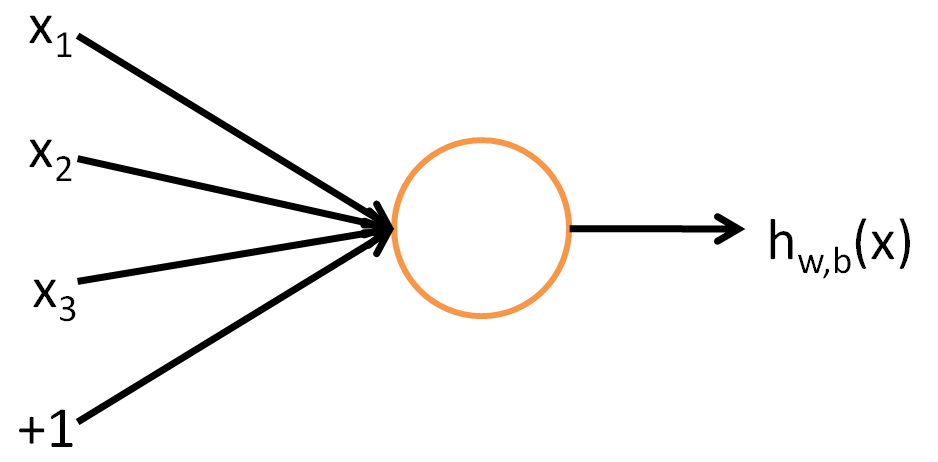
\includegraphics[width=0.5\textwidth]{figures/SingleNeuron.png}
  %\caption{}\label{fig:step1}
\end{figure}


\cnt{This ``neuron\index{neuron}" is a computational unit that takes as input $x_1,x_2,x_3$ (and a +1 intercept term), and outputs $h_{W,b}(x) = f(W^Tx) = f(\sum_{i=1}^3 W_{i}x_i +b)$, where $f : \Re \mapsto \Re$ is called the \emph{activation function}\index{activation function}. In these notes, we will choose $f(\cdot)$ to be the \index{sigmoid} function:}
    {这个“神经元\index{神经元}”是一个以 $x_1, x_2, x_3$ 及截距 $+1$ 为输入值的运算单元,其输出为 $h_{W,b}(x) = f(W^Tx) = f(\sum_{i=1}^3 W_{i}x_i +b)$,其中函数 $f : \Re \mapsto \Re$ 被称为“激活函数\index{激活函数}”。在本教程中,我们选用 sigmoid\index{sigmoid} 函数作为\emph{激活函数} $f(\cdot)$}
    {}

$$
f(z) = \frac{1}{1+\exp(-z)}.
$$

\cnt{Thus, our single neuron corresponds exactly to the input-output mapping defined by logistic regression.}
    {可以看出,这个单一“神经元”的输入-输出映射关系其实就是一个逻辑回归(logistic regression)。}
    {}
\cnt{Although these notes will use the sigmoid function, it is worth noting that another common choice for $f$ is the hyperbolic tangent\index{hyperbolic tangent}, or $\tanh$\index{tanh@$\tanh$}, function:}
    {虽然本系列教程采用sigmoid函数,但你也可以选择 双曲正切函数\index{双曲正切函数}($\tanh$\index{tanh@$\tanh$}):}
    {}

$$
f(z) = \tanh(z) = \frac{e^z - e^{-z}}{e^z + e^{-z}},
$$

%\cnt{Here are plots of the sigmoid(Figure \ref{fig:actfuncsig}) and $\tanh$ (Figure\ref{fig:actfunctanh}) functions:}
%    {以下图 \ref{fig:actfuncsig} 和 图 \ref{fig:actfunctanh} 分别是sigmoid及tanh的函数图像}
%    {}
\cnt{Here are plots of the sigmoid and $\tanh$ functions (Figure \ref{fig:actfuncs}):}
    {以下图 \ref{fig:actfuncs} 分别是 sigmoid 及 tanh 的函数图像}
    {}
\begin{figure}[ht] \centering
  % GNUPLOT: LaTeX picture
\setlength{\unitlength}{0.240900pt}
\ifx\plotpoint\undefined\newsavebox{\plotpoint}\fi
\sbox{\plotpoint}{\rule[-0.200pt]{0.400pt}{0.400pt}}%
\begin{picture}(1500,900)(0,0)
\sbox{\plotpoint}{\rule[-0.200pt]{0.400pt}{0.400pt}}%
\sbox{\plotpoint}{\rule[-0.500pt]{1.000pt}{1.000pt}}%
\multiput(191,164)(20.756,0.000){44}{\usebox{\plotpoint}}
\put(1099,164){\usebox{\plotpoint}}
\put(1419.00,164.00){\usebox{\plotpoint}}
\put(1439,164){\usebox{\plotpoint}}
\sbox{\plotpoint}{\rule[-0.200pt]{0.400pt}{0.400pt}}%
\put(191.0,164.0){\rule[-0.200pt]{4.818pt}{0.400pt}}
\put(171,164){\makebox(0,0)[r]{-1}}
\put(1419.0,164.0){\rule[-0.200pt]{4.818pt}{0.400pt}}
\sbox{\plotpoint}{\rule[-0.500pt]{1.000pt}{1.000pt}}%
\multiput(191,330)(20.756,0.000){44}{\usebox{\plotpoint}}
\put(1099,330){\usebox{\plotpoint}}
\put(1419.00,330.00){\usebox{\plotpoint}}
\put(1439,330){\usebox{\plotpoint}}
\sbox{\plotpoint}{\rule[-0.200pt]{0.400pt}{0.400pt}}%
\put(191.0,330.0){\rule[-0.200pt]{4.818pt}{0.400pt}}
\put(171,330){\makebox(0,0)[r]{-0.5}}
\put(1419.0,330.0){\rule[-0.200pt]{4.818pt}{0.400pt}}
\sbox{\plotpoint}{\rule[-0.500pt]{1.000pt}{1.000pt}}%
\multiput(191,495)(20.756,0.000){61}{\usebox{\plotpoint}}
\put(1439,495){\usebox{\plotpoint}}
\sbox{\plotpoint}{\rule[-0.200pt]{0.400pt}{0.400pt}}%
\put(191.0,495.0){\rule[-0.200pt]{4.818pt}{0.400pt}}
\put(171,495){\makebox(0,0)[r]{ 0}}
\put(1419.0,495.0){\rule[-0.200pt]{4.818pt}{0.400pt}}
\sbox{\plotpoint}{\rule[-0.500pt]{1.000pt}{1.000pt}}%
\multiput(191,660)(20.756,0.000){61}{\usebox{\plotpoint}}
\put(1439,660){\usebox{\plotpoint}}
\sbox{\plotpoint}{\rule[-0.200pt]{0.400pt}{0.400pt}}%
\put(191.0,660.0){\rule[-0.200pt]{4.818pt}{0.400pt}}
\put(171,660){\makebox(0,0)[r]{ 0.5}}
\put(1419.0,660.0){\rule[-0.200pt]{4.818pt}{0.400pt}}
\sbox{\plotpoint}{\rule[-0.500pt]{1.000pt}{1.000pt}}%
\multiput(191,826)(20.756,0.000){61}{\usebox{\plotpoint}}
\put(1439,826){\usebox{\plotpoint}}
\sbox{\plotpoint}{\rule[-0.200pt]{0.400pt}{0.400pt}}%
\put(191.0,826.0){\rule[-0.200pt]{4.818pt}{0.400pt}}
\put(171,826){\makebox(0,0)[r]{ 1}}
\put(1419.0,826.0){\rule[-0.200pt]{4.818pt}{0.400pt}}
\sbox{\plotpoint}{\rule[-0.500pt]{1.000pt}{1.000pt}}%
\multiput(326,131)(0.000,20.756){36}{\usebox{\plotpoint}}
\put(326,859){\usebox{\plotpoint}}
\sbox{\plotpoint}{\rule[-0.200pt]{0.400pt}{0.400pt}}%
\put(326.0,131.0){\rule[-0.200pt]{0.400pt}{4.818pt}}
\put(326,90){\makebox(0,0){-4}}
\put(326.0,839.0){\rule[-0.200pt]{0.400pt}{4.818pt}}
\sbox{\plotpoint}{\rule[-0.500pt]{1.000pt}{1.000pt}}%
\multiput(570,131)(0.000,20.756){36}{\usebox{\plotpoint}}
\put(570,859){\usebox{\plotpoint}}
\sbox{\plotpoint}{\rule[-0.200pt]{0.400pt}{0.400pt}}%
\put(570.0,131.0){\rule[-0.200pt]{0.400pt}{4.818pt}}
\put(570,90){\makebox(0,0){-2}}
\put(570.0,839.0){\rule[-0.200pt]{0.400pt}{4.818pt}}
\sbox{\plotpoint}{\rule[-0.500pt]{1.000pt}{1.000pt}}%
\multiput(815,131)(0.000,20.756){36}{\usebox{\plotpoint}}
\put(815,859){\usebox{\plotpoint}}
\sbox{\plotpoint}{\rule[-0.200pt]{0.400pt}{0.400pt}}%
\put(815.0,131.0){\rule[-0.200pt]{0.400pt}{4.818pt}}
\put(815,90){\makebox(0,0){ 0}}
\put(815.0,839.0){\rule[-0.200pt]{0.400pt}{4.818pt}}
\sbox{\plotpoint}{\rule[-0.500pt]{1.000pt}{1.000pt}}%
\multiput(1060,131)(0.000,20.756){36}{\usebox{\plotpoint}}
\put(1060,859){\usebox{\plotpoint}}
\sbox{\plotpoint}{\rule[-0.200pt]{0.400pt}{0.400pt}}%
\put(1060.0,131.0){\rule[-0.200pt]{0.400pt}{4.818pt}}
\put(1060,90){\makebox(0,0){ 2}}
\put(1060.0,839.0){\rule[-0.200pt]{0.400pt}{4.818pt}}
\sbox{\plotpoint}{\rule[-0.500pt]{1.000pt}{1.000pt}}%
\put(1304.00,131.00){\usebox{\plotpoint}}
\put(1304,151){\usebox{\plotpoint}}
\multiput(1304,351)(0.000,20.756){25}{\usebox{\plotpoint}}
\put(1304,859){\usebox{\plotpoint}}
\sbox{\plotpoint}{\rule[-0.200pt]{0.400pt}{0.400pt}}%
\put(1304.0,131.0){\rule[-0.200pt]{0.400pt}{4.818pt}}
\put(1304,90){\makebox(0,0){ 4}}
\put(1304.0,839.0){\rule[-0.200pt]{0.400pt}{4.818pt}}
\put(191.0,131.0){\rule[-0.200pt]{0.400pt}{175.375pt}}
\put(191.0,131.0){\rule[-0.200pt]{300.643pt}{0.400pt}}
\put(1439.0,131.0){\rule[-0.200pt]{0.400pt}{175.375pt}}
\put(191.0,859.0){\rule[-0.200pt]{300.643pt}{0.400pt}}
\put(30,495){\makebox(0,0){$f(z)$}}
\put(815,29){\makebox(0,0){$z$}}
\put(1099.0,151.0){\rule[-0.200pt]{0.400pt}{48.180pt}}
\put(1099.0,351.0){\rule[-0.200pt]{77.088pt}{0.400pt}}
\put(1419.0,151.0){\rule[-0.200pt]{0.400pt}{48.180pt}}
\put(1099.0,151.0){\rule[-0.200pt]{77.088pt}{0.400pt}}
\put(1279,301){\makebox(0,0)[r]{$\frac{1}{1+\exp(-z)}$}}
\put(1299.0,301.0){\rule[-0.200pt]{24.090pt}{0.400pt}}
\put(191,497){\usebox{\plotpoint}}
\put(216,496.67){\rule{3.132pt}{0.400pt}}
\multiput(216.00,496.17)(6.500,1.000){2}{\rule{1.566pt}{0.400pt}}
\put(191.0,497.0){\rule[-0.200pt]{6.022pt}{0.400pt}}
\put(254,497.67){\rule{3.132pt}{0.400pt}}
\multiput(254.00,497.17)(6.500,1.000){2}{\rule{1.566pt}{0.400pt}}
\put(229.0,498.0){\rule[-0.200pt]{6.022pt}{0.400pt}}
\put(279,498.67){\rule{3.132pt}{0.400pt}}
\multiput(279.00,498.17)(6.500,1.000){2}{\rule{1.566pt}{0.400pt}}
\put(267.0,499.0){\rule[-0.200pt]{2.891pt}{0.400pt}}
\put(304,499.67){\rule{3.132pt}{0.400pt}}
\multiput(304.00,499.17)(6.500,1.000){2}{\rule{1.566pt}{0.400pt}}
\put(292.0,500.0){\rule[-0.200pt]{2.891pt}{0.400pt}}
\put(330,500.67){\rule{2.891pt}{0.400pt}}
\multiput(330.00,500.17)(6.000,1.000){2}{\rule{1.445pt}{0.400pt}}
\put(342,501.67){\rule{3.132pt}{0.400pt}}
\multiput(342.00,501.17)(6.500,1.000){2}{\rule{1.566pt}{0.400pt}}
\put(317.0,501.0){\rule[-0.200pt]{3.132pt}{0.400pt}}
\put(367,502.67){\rule{3.132pt}{0.400pt}}
\multiput(367.00,502.17)(6.500,1.000){2}{\rule{1.566pt}{0.400pt}}
\put(380,503.67){\rule{3.132pt}{0.400pt}}
\multiput(380.00,503.17)(6.500,1.000){2}{\rule{1.566pt}{0.400pt}}
\put(393,504.67){\rule{2.891pt}{0.400pt}}
\multiput(393.00,504.17)(6.000,1.000){2}{\rule{1.445pt}{0.400pt}}
\put(405,505.67){\rule{3.132pt}{0.400pt}}
\multiput(405.00,505.17)(6.500,1.000){2}{\rule{1.566pt}{0.400pt}}
\put(418,507.17){\rule{2.700pt}{0.400pt}}
\multiput(418.00,506.17)(7.396,2.000){2}{\rule{1.350pt}{0.400pt}}
\put(431,508.67){\rule{2.891pt}{0.400pt}}
\multiput(431.00,508.17)(6.000,1.000){2}{\rule{1.445pt}{0.400pt}}
\put(443,510.17){\rule{2.700pt}{0.400pt}}
\multiput(443.00,509.17)(7.396,2.000){2}{\rule{1.350pt}{0.400pt}}
\put(456,511.67){\rule{2.891pt}{0.400pt}}
\multiput(456.00,511.17)(6.000,1.000){2}{\rule{1.445pt}{0.400pt}}
\put(468,513.17){\rule{2.700pt}{0.400pt}}
\multiput(468.00,512.17)(7.396,2.000){2}{\rule{1.350pt}{0.400pt}}
\put(481,515.17){\rule{2.700pt}{0.400pt}}
\multiput(481.00,514.17)(7.396,2.000){2}{\rule{1.350pt}{0.400pt}}
\multiput(494.00,517.61)(2.472,0.447){3}{\rule{1.700pt}{0.108pt}}
\multiput(494.00,516.17)(8.472,3.000){2}{\rule{0.850pt}{0.400pt}}
\put(506,520.17){\rule{2.700pt}{0.400pt}}
\multiput(506.00,519.17)(7.396,2.000){2}{\rule{1.350pt}{0.400pt}}
\multiput(519.00,522.61)(2.472,0.447){3}{\rule{1.700pt}{0.108pt}}
\multiput(519.00,521.17)(8.472,3.000){2}{\rule{0.850pt}{0.400pt}}
\multiput(531.00,525.61)(2.695,0.447){3}{\rule{1.833pt}{0.108pt}}
\multiput(531.00,524.17)(9.195,3.000){2}{\rule{0.917pt}{0.400pt}}
\multiput(544.00,528.61)(2.695,0.447){3}{\rule{1.833pt}{0.108pt}}
\multiput(544.00,527.17)(9.195,3.000){2}{\rule{0.917pt}{0.400pt}}
\multiput(557.00,531.61)(2.472,0.447){3}{\rule{1.700pt}{0.108pt}}
\multiput(557.00,530.17)(8.472,3.000){2}{\rule{0.850pt}{0.400pt}}
\multiput(569.00,534.60)(1.797,0.468){5}{\rule{1.400pt}{0.113pt}}
\multiput(569.00,533.17)(10.094,4.000){2}{\rule{0.700pt}{0.400pt}}
\multiput(582.00,538.60)(1.651,0.468){5}{\rule{1.300pt}{0.113pt}}
\multiput(582.00,537.17)(9.302,4.000){2}{\rule{0.650pt}{0.400pt}}
\multiput(594.00,542.60)(1.797,0.468){5}{\rule{1.400pt}{0.113pt}}
\multiput(594.00,541.17)(10.094,4.000){2}{\rule{0.700pt}{0.400pt}}
\multiput(607.00,546.59)(1.378,0.477){7}{\rule{1.140pt}{0.115pt}}
\multiput(607.00,545.17)(10.634,5.000){2}{\rule{0.570pt}{0.400pt}}
\multiput(620.00,551.59)(1.267,0.477){7}{\rule{1.060pt}{0.115pt}}
\multiput(620.00,550.17)(9.800,5.000){2}{\rule{0.530pt}{0.400pt}}
\multiput(632.00,556.59)(1.378,0.477){7}{\rule{1.140pt}{0.115pt}}
\multiput(632.00,555.17)(10.634,5.000){2}{\rule{0.570pt}{0.400pt}}
\multiput(645.00,561.59)(1.033,0.482){9}{\rule{0.900pt}{0.116pt}}
\multiput(645.00,560.17)(10.132,6.000){2}{\rule{0.450pt}{0.400pt}}
\multiput(657.00,567.59)(1.378,0.477){7}{\rule{1.140pt}{0.115pt}}
\multiput(657.00,566.17)(10.634,5.000){2}{\rule{0.570pt}{0.400pt}}
\multiput(670.00,572.59)(0.950,0.485){11}{\rule{0.843pt}{0.117pt}}
\multiput(670.00,571.17)(11.251,7.000){2}{\rule{0.421pt}{0.400pt}}
\multiput(683.00,579.59)(1.033,0.482){9}{\rule{0.900pt}{0.116pt}}
\multiput(683.00,578.17)(10.132,6.000){2}{\rule{0.450pt}{0.400pt}}
\multiput(695.00,585.59)(0.950,0.485){11}{\rule{0.843pt}{0.117pt}}
\multiput(695.00,584.17)(11.251,7.000){2}{\rule{0.421pt}{0.400pt}}
\multiput(708.00,592.59)(0.758,0.488){13}{\rule{0.700pt}{0.117pt}}
\multiput(708.00,591.17)(10.547,8.000){2}{\rule{0.350pt}{0.400pt}}
\multiput(720.00,600.59)(0.950,0.485){11}{\rule{0.843pt}{0.117pt}}
\multiput(720.00,599.17)(11.251,7.000){2}{\rule{0.421pt}{0.400pt}}
\multiput(733.00,607.59)(0.824,0.488){13}{\rule{0.750pt}{0.117pt}}
\multiput(733.00,606.17)(11.443,8.000){2}{\rule{0.375pt}{0.400pt}}
\multiput(746.00,615.59)(0.758,0.488){13}{\rule{0.700pt}{0.117pt}}
\multiput(746.00,614.17)(10.547,8.000){2}{\rule{0.350pt}{0.400pt}}
\multiput(758.00,623.59)(0.824,0.488){13}{\rule{0.750pt}{0.117pt}}
\multiput(758.00,622.17)(11.443,8.000){2}{\rule{0.375pt}{0.400pt}}
\multiput(771.00,631.59)(0.758,0.488){13}{\rule{0.700pt}{0.117pt}}
\multiput(771.00,630.17)(10.547,8.000){2}{\rule{0.350pt}{0.400pt}}
\multiput(783.00,639.59)(0.728,0.489){15}{\rule{0.678pt}{0.118pt}}
\multiput(783.00,638.17)(11.593,9.000){2}{\rule{0.339pt}{0.400pt}}
\multiput(796.00,648.59)(0.824,0.488){13}{\rule{0.750pt}{0.117pt}}
\multiput(796.00,647.17)(11.443,8.000){2}{\rule{0.375pt}{0.400pt}}
\multiput(809.00,656.59)(0.669,0.489){15}{\rule{0.633pt}{0.118pt}}
\multiput(809.00,655.17)(10.685,9.000){2}{\rule{0.317pt}{0.400pt}}
\multiput(821.00,665.59)(0.824,0.488){13}{\rule{0.750pt}{0.117pt}}
\multiput(821.00,664.17)(11.443,8.000){2}{\rule{0.375pt}{0.400pt}}
\multiput(834.00,673.59)(0.728,0.489){15}{\rule{0.678pt}{0.118pt}}
\multiput(834.00,672.17)(11.593,9.000){2}{\rule{0.339pt}{0.400pt}}
\multiput(847.00,682.59)(0.758,0.488){13}{\rule{0.700pt}{0.117pt}}
\multiput(847.00,681.17)(10.547,8.000){2}{\rule{0.350pt}{0.400pt}}
\multiput(859.00,690.59)(0.824,0.488){13}{\rule{0.750pt}{0.117pt}}
\multiput(859.00,689.17)(11.443,8.000){2}{\rule{0.375pt}{0.400pt}}
\multiput(872.00,698.59)(0.758,0.488){13}{\rule{0.700pt}{0.117pt}}
\multiput(872.00,697.17)(10.547,8.000){2}{\rule{0.350pt}{0.400pt}}
\multiput(884.00,706.59)(0.824,0.488){13}{\rule{0.750pt}{0.117pt}}
\multiput(884.00,705.17)(11.443,8.000){2}{\rule{0.375pt}{0.400pt}}
\multiput(897.00,714.59)(0.950,0.485){11}{\rule{0.843pt}{0.117pt}}
\multiput(897.00,713.17)(11.251,7.000){2}{\rule{0.421pt}{0.400pt}}
\multiput(910.00,721.59)(0.758,0.488){13}{\rule{0.700pt}{0.117pt}}
\multiput(910.00,720.17)(10.547,8.000){2}{\rule{0.350pt}{0.400pt}}
\multiput(922.00,729.59)(0.950,0.485){11}{\rule{0.843pt}{0.117pt}}
\multiput(922.00,728.17)(11.251,7.000){2}{\rule{0.421pt}{0.400pt}}
\multiput(935.00,736.59)(1.033,0.482){9}{\rule{0.900pt}{0.116pt}}
\multiput(935.00,735.17)(10.132,6.000){2}{\rule{0.450pt}{0.400pt}}
\multiput(947.00,742.59)(1.123,0.482){9}{\rule{0.967pt}{0.116pt}}
\multiput(947.00,741.17)(10.994,6.000){2}{\rule{0.483pt}{0.400pt}}
\multiput(960.00,748.59)(1.123,0.482){9}{\rule{0.967pt}{0.116pt}}
\multiput(960.00,747.17)(10.994,6.000){2}{\rule{0.483pt}{0.400pt}}
\multiput(973.00,754.59)(1.033,0.482){9}{\rule{0.900pt}{0.116pt}}
\multiput(973.00,753.17)(10.132,6.000){2}{\rule{0.450pt}{0.400pt}}
\multiput(985.00,760.59)(1.378,0.477){7}{\rule{1.140pt}{0.115pt}}
\multiput(985.00,759.17)(10.634,5.000){2}{\rule{0.570pt}{0.400pt}}
\multiput(998.00,765.59)(1.267,0.477){7}{\rule{1.060pt}{0.115pt}}
\multiput(998.00,764.17)(9.800,5.000){2}{\rule{0.530pt}{0.400pt}}
\multiput(1010.00,770.59)(1.378,0.477){7}{\rule{1.140pt}{0.115pt}}
\multiput(1010.00,769.17)(10.634,5.000){2}{\rule{0.570pt}{0.400pt}}
\multiput(1023.00,775.60)(1.797,0.468){5}{\rule{1.400pt}{0.113pt}}
\multiput(1023.00,774.17)(10.094,4.000){2}{\rule{0.700pt}{0.400pt}}
\multiput(1036.00,779.60)(1.651,0.468){5}{\rule{1.300pt}{0.113pt}}
\multiput(1036.00,778.17)(9.302,4.000){2}{\rule{0.650pt}{0.400pt}}
\multiput(1048.00,783.60)(1.797,0.468){5}{\rule{1.400pt}{0.113pt}}
\multiput(1048.00,782.17)(10.094,4.000){2}{\rule{0.700pt}{0.400pt}}
\multiput(1061.00,787.61)(2.472,0.447){3}{\rule{1.700pt}{0.108pt}}
\multiput(1061.00,786.17)(8.472,3.000){2}{\rule{0.850pt}{0.400pt}}
\multiput(1073.00,790.61)(2.695,0.447){3}{\rule{1.833pt}{0.108pt}}
\multiput(1073.00,789.17)(9.195,3.000){2}{\rule{0.917pt}{0.400pt}}
\multiput(1086.00,793.61)(2.695,0.447){3}{\rule{1.833pt}{0.108pt}}
\multiput(1086.00,792.17)(9.195,3.000){2}{\rule{0.917pt}{0.400pt}}
\multiput(1099.00,796.61)(2.472,0.447){3}{\rule{1.700pt}{0.108pt}}
\multiput(1099.00,795.17)(8.472,3.000){2}{\rule{0.850pt}{0.400pt}}
\put(1111,799.17){\rule{2.700pt}{0.400pt}}
\multiput(1111.00,798.17)(7.396,2.000){2}{\rule{1.350pt}{0.400pt}}
\multiput(1124.00,801.61)(2.472,0.447){3}{\rule{1.700pt}{0.108pt}}
\multiput(1124.00,800.17)(8.472,3.000){2}{\rule{0.850pt}{0.400pt}}
\put(1136,804.17){\rule{2.700pt}{0.400pt}}
\multiput(1136.00,803.17)(7.396,2.000){2}{\rule{1.350pt}{0.400pt}}
\put(1149,806.17){\rule{2.700pt}{0.400pt}}
\multiput(1149.00,805.17)(7.396,2.000){2}{\rule{1.350pt}{0.400pt}}
\put(1162,807.67){\rule{2.891pt}{0.400pt}}
\multiput(1162.00,807.17)(6.000,1.000){2}{\rule{1.445pt}{0.400pt}}
\put(1174,809.17){\rule{2.700pt}{0.400pt}}
\multiput(1174.00,808.17)(7.396,2.000){2}{\rule{1.350pt}{0.400pt}}
\put(1187,810.67){\rule{2.891pt}{0.400pt}}
\multiput(1187.00,810.17)(6.000,1.000){2}{\rule{1.445pt}{0.400pt}}
\put(1199,812.17){\rule{2.700pt}{0.400pt}}
\multiput(1199.00,811.17)(7.396,2.000){2}{\rule{1.350pt}{0.400pt}}
\put(1212,813.67){\rule{3.132pt}{0.400pt}}
\multiput(1212.00,813.17)(6.500,1.000){2}{\rule{1.566pt}{0.400pt}}
\put(1225,814.67){\rule{2.891pt}{0.400pt}}
\multiput(1225.00,814.17)(6.000,1.000){2}{\rule{1.445pt}{0.400pt}}
\put(1237,815.67){\rule{3.132pt}{0.400pt}}
\multiput(1237.00,815.17)(6.500,1.000){2}{\rule{1.566pt}{0.400pt}}
\put(1250,816.67){\rule{3.132pt}{0.400pt}}
\multiput(1250.00,816.17)(6.500,1.000){2}{\rule{1.566pt}{0.400pt}}
\put(355.0,503.0){\rule[-0.200pt]{2.891pt}{0.400pt}}
\put(1275,817.67){\rule{3.132pt}{0.400pt}}
\multiput(1275.00,817.17)(6.500,1.000){2}{\rule{1.566pt}{0.400pt}}
\put(1288,818.67){\rule{2.891pt}{0.400pt}}
\multiput(1288.00,818.17)(6.000,1.000){2}{\rule{1.445pt}{0.400pt}}
\put(1263.0,818.0){\rule[-0.200pt]{2.891pt}{0.400pt}}
\put(1313,819.67){\rule{3.132pt}{0.400pt}}
\multiput(1313.00,819.17)(6.500,1.000){2}{\rule{1.566pt}{0.400pt}}
\put(1300.0,820.0){\rule[-0.200pt]{3.132pt}{0.400pt}}
\put(1338,820.67){\rule{3.132pt}{0.400pt}}
\multiput(1338.00,820.17)(6.500,1.000){2}{\rule{1.566pt}{0.400pt}}
\put(1326.0,821.0){\rule[-0.200pt]{2.891pt}{0.400pt}}
\put(1363,821.67){\rule{3.132pt}{0.400pt}}
\multiput(1363.00,821.17)(6.500,1.000){2}{\rule{1.566pt}{0.400pt}}
\put(1351.0,822.0){\rule[-0.200pt]{2.891pt}{0.400pt}}
\put(1414,822.67){\rule{2.891pt}{0.400pt}}
\multiput(1414.00,822.17)(6.000,1.000){2}{\rule{1.445pt}{0.400pt}}
\put(1376.0,823.0){\rule[-0.200pt]{9.154pt}{0.400pt}}
\put(1426.0,824.0){\rule[-0.200pt]{3.132pt}{0.400pt}}
\sbox{\plotpoint}{\rule[-0.400pt]{0.800pt}{0.800pt}}%
\sbox{\plotpoint}{\rule[-0.200pt]{0.400pt}{0.400pt}}%
\put(1279,201){\makebox(0,0)[r]{$\tanh(z)$}}
\sbox{\plotpoint}{\rule[-0.400pt]{0.800pt}{0.800pt}}%
\put(1299.0,201.0){\rule[-0.400pt]{24.090pt}{0.800pt}}
\put(191,164){\usebox{\plotpoint}}
\put(355,162.84){\rule{2.891pt}{0.800pt}}
\multiput(355.00,162.34)(6.000,1.000){2}{\rule{1.445pt}{0.800pt}}
\put(191.0,164.0){\rule[-0.400pt]{39.508pt}{0.800pt}}
\put(431,163.84){\rule{2.891pt}{0.800pt}}
\multiput(431.00,163.34)(6.000,1.000){2}{\rule{1.445pt}{0.800pt}}
\put(367.0,165.0){\rule[-0.400pt]{15.418pt}{0.800pt}}
\put(468,164.84){\rule{3.132pt}{0.800pt}}
\multiput(468.00,164.34)(6.500,1.000){2}{\rule{1.566pt}{0.800pt}}
\put(481,165.84){\rule{3.132pt}{0.800pt}}
\multiput(481.00,165.34)(6.500,1.000){2}{\rule{1.566pt}{0.800pt}}
\put(443.0,166.0){\rule[-0.400pt]{6.022pt}{0.800pt}}
\put(506,166.84){\rule{3.132pt}{0.800pt}}
\multiput(506.00,166.34)(6.500,1.000){2}{\rule{1.566pt}{0.800pt}}
\put(519,167.84){\rule{2.891pt}{0.800pt}}
\multiput(519.00,167.34)(6.000,1.000){2}{\rule{1.445pt}{0.800pt}}
\put(531,169.34){\rule{3.132pt}{0.800pt}}
\multiput(531.00,168.34)(6.500,2.000){2}{\rule{1.566pt}{0.800pt}}
\put(544,171.34){\rule{3.132pt}{0.800pt}}
\multiput(544.00,170.34)(6.500,2.000){2}{\rule{1.566pt}{0.800pt}}
\put(557,173.34){\rule{2.891pt}{0.800pt}}
\multiput(557.00,172.34)(6.000,2.000){2}{\rule{1.445pt}{0.800pt}}
\put(569,175.34){\rule{3.132pt}{0.800pt}}
\multiput(569.00,174.34)(6.500,2.000){2}{\rule{1.566pt}{0.800pt}}
\put(582,178.34){\rule{2.600pt}{0.800pt}}
\multiput(582.00,176.34)(6.604,4.000){2}{\rule{1.300pt}{0.800pt}}
\put(594,181.84){\rule{3.132pt}{0.800pt}}
\multiput(594.00,180.34)(6.500,3.000){2}{\rule{1.566pt}{0.800pt}}
\multiput(607.00,186.38)(1.768,0.560){3}{\rule{2.280pt}{0.135pt}}
\multiput(607.00,183.34)(8.268,5.000){2}{\rule{1.140pt}{0.800pt}}
\multiput(620.00,191.39)(1.132,0.536){5}{\rule{1.800pt}{0.129pt}}
\multiput(620.00,188.34)(8.264,6.000){2}{\rule{0.900pt}{0.800pt}}
\multiput(632.00,197.40)(1.000,0.526){7}{\rule{1.686pt}{0.127pt}}
\multiput(632.00,194.34)(9.501,7.000){2}{\rule{0.843pt}{0.800pt}}
\multiput(645.00,204.40)(0.774,0.520){9}{\rule{1.400pt}{0.125pt}}
\multiput(645.00,201.34)(9.094,8.000){2}{\rule{0.700pt}{0.800pt}}
\multiput(657.00,212.40)(0.654,0.514){13}{\rule{1.240pt}{0.124pt}}
\multiput(657.00,209.34)(10.426,10.000){2}{\rule{0.620pt}{0.800pt}}
\multiput(670.00,222.40)(0.589,0.512){15}{\rule{1.145pt}{0.123pt}}
\multiput(670.00,219.34)(10.623,11.000){2}{\rule{0.573pt}{0.800pt}}
\multiput(684.41,232.00)(0.511,0.581){17}{\rule{0.123pt}{1.133pt}}
\multiput(681.34,232.00)(12.000,11.648){2}{\rule{0.800pt}{0.567pt}}
\multiput(696.41,246.00)(0.509,0.616){19}{\rule{0.123pt}{1.185pt}}
\multiput(693.34,246.00)(13.000,13.541){2}{\rule{0.800pt}{0.592pt}}
\multiput(709.41,262.00)(0.511,0.762){17}{\rule{0.123pt}{1.400pt}}
\multiput(706.34,262.00)(12.000,15.094){2}{\rule{0.800pt}{0.700pt}}
\multiput(721.41,280.00)(0.509,0.823){19}{\rule{0.123pt}{1.492pt}}
\multiput(718.34,280.00)(13.000,17.903){2}{\rule{0.800pt}{0.746pt}}
\multiput(734.41,301.00)(0.509,0.947){19}{\rule{0.123pt}{1.677pt}}
\multiput(731.34,301.00)(13.000,20.519){2}{\rule{0.800pt}{0.838pt}}
\multiput(747.41,325.00)(0.511,1.169){17}{\rule{0.123pt}{2.000pt}}
\multiput(744.34,325.00)(12.000,22.849){2}{\rule{0.800pt}{1.000pt}}
\multiput(759.41,352.00)(0.509,1.153){19}{\rule{0.123pt}{1.985pt}}
\multiput(756.34,352.00)(13.000,24.881){2}{\rule{0.800pt}{0.992pt}}
\multiput(772.41,381.00)(0.511,1.349){17}{\rule{0.123pt}{2.267pt}}
\multiput(769.34,381.00)(12.000,26.295){2}{\rule{0.800pt}{1.133pt}}
\multiput(784.41,412.00)(0.509,1.278){19}{\rule{0.123pt}{2.169pt}}
\multiput(781.34,412.00)(13.000,27.498){2}{\rule{0.800pt}{1.085pt}}
\multiput(797.41,444.00)(0.509,1.360){19}{\rule{0.123pt}{2.292pt}}
\multiput(794.34,444.00)(13.000,29.242){2}{\rule{0.800pt}{1.146pt}}
\multiput(810.41,478.00)(0.511,1.485){17}{\rule{0.123pt}{2.467pt}}
\multiput(807.34,478.00)(12.000,28.880){2}{\rule{0.800pt}{1.233pt}}
\multiput(822.41,512.00)(0.509,1.360){19}{\rule{0.123pt}{2.292pt}}
\multiput(819.34,512.00)(13.000,29.242){2}{\rule{0.800pt}{1.146pt}}
\multiput(835.41,546.00)(0.509,1.278){19}{\rule{0.123pt}{2.169pt}}
\multiput(832.34,546.00)(13.000,27.498){2}{\rule{0.800pt}{1.085pt}}
\multiput(848.41,578.00)(0.511,1.349){17}{\rule{0.123pt}{2.267pt}}
\multiput(845.34,578.00)(12.000,26.295){2}{\rule{0.800pt}{1.133pt}}
\multiput(860.41,609.00)(0.509,1.153){19}{\rule{0.123pt}{1.985pt}}
\multiput(857.34,609.00)(13.000,24.881){2}{\rule{0.800pt}{0.992pt}}
\multiput(873.41,638.00)(0.511,1.169){17}{\rule{0.123pt}{2.000pt}}
\multiput(870.34,638.00)(12.000,22.849){2}{\rule{0.800pt}{1.000pt}}
\multiput(885.41,665.00)(0.509,0.947){19}{\rule{0.123pt}{1.677pt}}
\multiput(882.34,665.00)(13.000,20.519){2}{\rule{0.800pt}{0.838pt}}
\multiput(898.41,689.00)(0.509,0.823){19}{\rule{0.123pt}{1.492pt}}
\multiput(895.34,689.00)(13.000,17.903){2}{\rule{0.800pt}{0.746pt}}
\multiput(911.41,710.00)(0.511,0.762){17}{\rule{0.123pt}{1.400pt}}
\multiput(908.34,710.00)(12.000,15.094){2}{\rule{0.800pt}{0.700pt}}
\multiput(923.41,728.00)(0.509,0.616){19}{\rule{0.123pt}{1.185pt}}
\multiput(920.34,728.00)(13.000,13.541){2}{\rule{0.800pt}{0.592pt}}
\multiput(936.41,744.00)(0.511,0.581){17}{\rule{0.123pt}{1.133pt}}
\multiput(933.34,744.00)(12.000,11.648){2}{\rule{0.800pt}{0.567pt}}
\multiput(947.00,759.40)(0.589,0.512){15}{\rule{1.145pt}{0.123pt}}
\multiput(947.00,756.34)(10.623,11.000){2}{\rule{0.573pt}{0.800pt}}
\multiput(960.00,770.40)(0.654,0.514){13}{\rule{1.240pt}{0.124pt}}
\multiput(960.00,767.34)(10.426,10.000){2}{\rule{0.620pt}{0.800pt}}
\multiput(973.00,780.40)(0.774,0.520){9}{\rule{1.400pt}{0.125pt}}
\multiput(973.00,777.34)(9.094,8.000){2}{\rule{0.700pt}{0.800pt}}
\multiput(985.00,788.40)(1.000,0.526){7}{\rule{1.686pt}{0.127pt}}
\multiput(985.00,785.34)(9.501,7.000){2}{\rule{0.843pt}{0.800pt}}
\multiput(998.00,795.39)(1.132,0.536){5}{\rule{1.800pt}{0.129pt}}
\multiput(998.00,792.34)(8.264,6.000){2}{\rule{0.900pt}{0.800pt}}
\multiput(1010.00,801.38)(1.768,0.560){3}{\rule{2.280pt}{0.135pt}}
\multiput(1010.00,798.34)(8.268,5.000){2}{\rule{1.140pt}{0.800pt}}
\put(1023,804.84){\rule{3.132pt}{0.800pt}}
\multiput(1023.00,803.34)(6.500,3.000){2}{\rule{1.566pt}{0.800pt}}
\put(1036,808.34){\rule{2.600pt}{0.800pt}}
\multiput(1036.00,806.34)(6.604,4.000){2}{\rule{1.300pt}{0.800pt}}
\put(1048,811.34){\rule{3.132pt}{0.800pt}}
\multiput(1048.00,810.34)(6.500,2.000){2}{\rule{1.566pt}{0.800pt}}
\put(1061,813.34){\rule{2.891pt}{0.800pt}}
\multiput(1061.00,812.34)(6.000,2.000){2}{\rule{1.445pt}{0.800pt}}
\put(1073,815.34){\rule{3.132pt}{0.800pt}}
\multiput(1073.00,814.34)(6.500,2.000){2}{\rule{1.566pt}{0.800pt}}
\put(1086,817.34){\rule{3.132pt}{0.800pt}}
\multiput(1086.00,816.34)(6.500,2.000){2}{\rule{1.566pt}{0.800pt}}
\put(1099,818.84){\rule{2.891pt}{0.800pt}}
\multiput(1099.00,818.34)(6.000,1.000){2}{\rule{1.445pt}{0.800pt}}
\put(1111,819.84){\rule{3.132pt}{0.800pt}}
\multiput(1111.00,819.34)(6.500,1.000){2}{\rule{1.566pt}{0.800pt}}
\put(494.0,168.0){\rule[-0.400pt]{2.891pt}{0.800pt}}
\put(1136,820.84){\rule{3.132pt}{0.800pt}}
\multiput(1136.00,820.34)(6.500,1.000){2}{\rule{1.566pt}{0.800pt}}
\put(1149,821.84){\rule{3.132pt}{0.800pt}}
\multiput(1149.00,821.34)(6.500,1.000){2}{\rule{1.566pt}{0.800pt}}
\put(1124.0,822.0){\rule[-0.400pt]{2.891pt}{0.800pt}}
\put(1187,822.84){\rule{2.891pt}{0.800pt}}
\multiput(1187.00,822.34)(6.000,1.000){2}{\rule{1.445pt}{0.800pt}}
\put(1162.0,824.0){\rule[-0.400pt]{6.022pt}{0.800pt}}
\put(1263,823.84){\rule{2.891pt}{0.800pt}}
\multiput(1263.00,823.34)(6.000,1.000){2}{\rule{1.445pt}{0.800pt}}
\put(1199.0,825.0){\rule[-0.400pt]{15.418pt}{0.800pt}}
\put(1275.0,826.0){\rule[-0.400pt]{39.508pt}{0.800pt}}
\put(815,495){\usebox{\plotpoint}}
\put(815,495){\makebox(0,0){$\bullet$}}
\sbox{\plotpoint}{\rule[-0.500pt]{1.000pt}{1.000pt}}%
\put(815,660){\usebox{\plotpoint}}
\put(815,660){\usebox{\plotpoint}}
\put(815,660){\makebox(0,0){$\bullet$}}
\sbox{\plotpoint}{\rule[-0.200pt]{0.400pt}{0.400pt}}%
\put(191.0,131.0){\rule[-0.200pt]{0.400pt}{175.375pt}}
\put(191.0,131.0){\rule[-0.200pt]{300.643pt}{0.400pt}}
\put(1439.0,131.0){\rule[-0.200pt]{0.400pt}{175.375pt}}
\put(191.0,859.0){\rule[-0.200pt]{300.643pt}{0.400pt}}
\end{picture}

  \caption{\cnt{Activation functions}{激活函数}{}}\label{fig:actfuncs}
\end{figure}

%\begin{figure}[ht] \centering
%  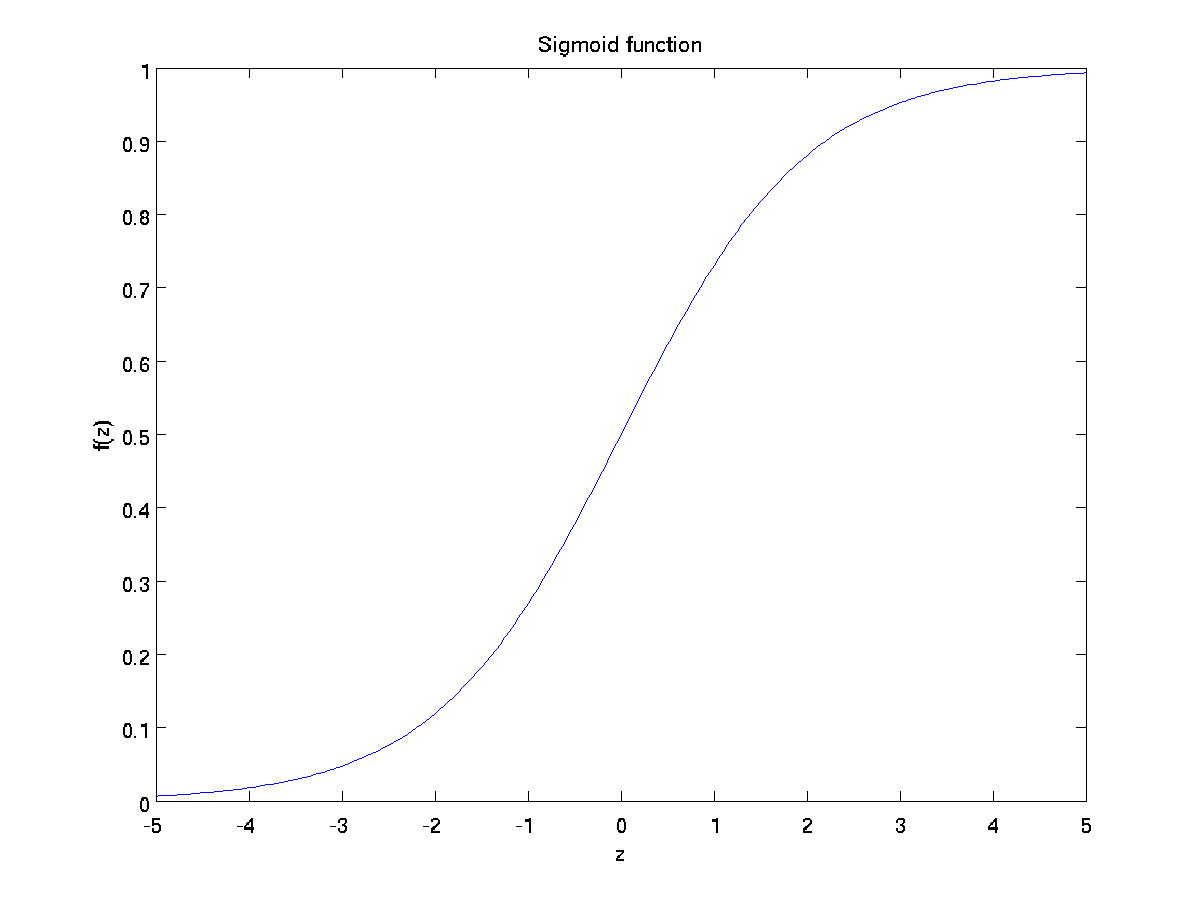
\includegraphics[width=0.45\textwidth]{figures/Sigmoid_Function.png}
%  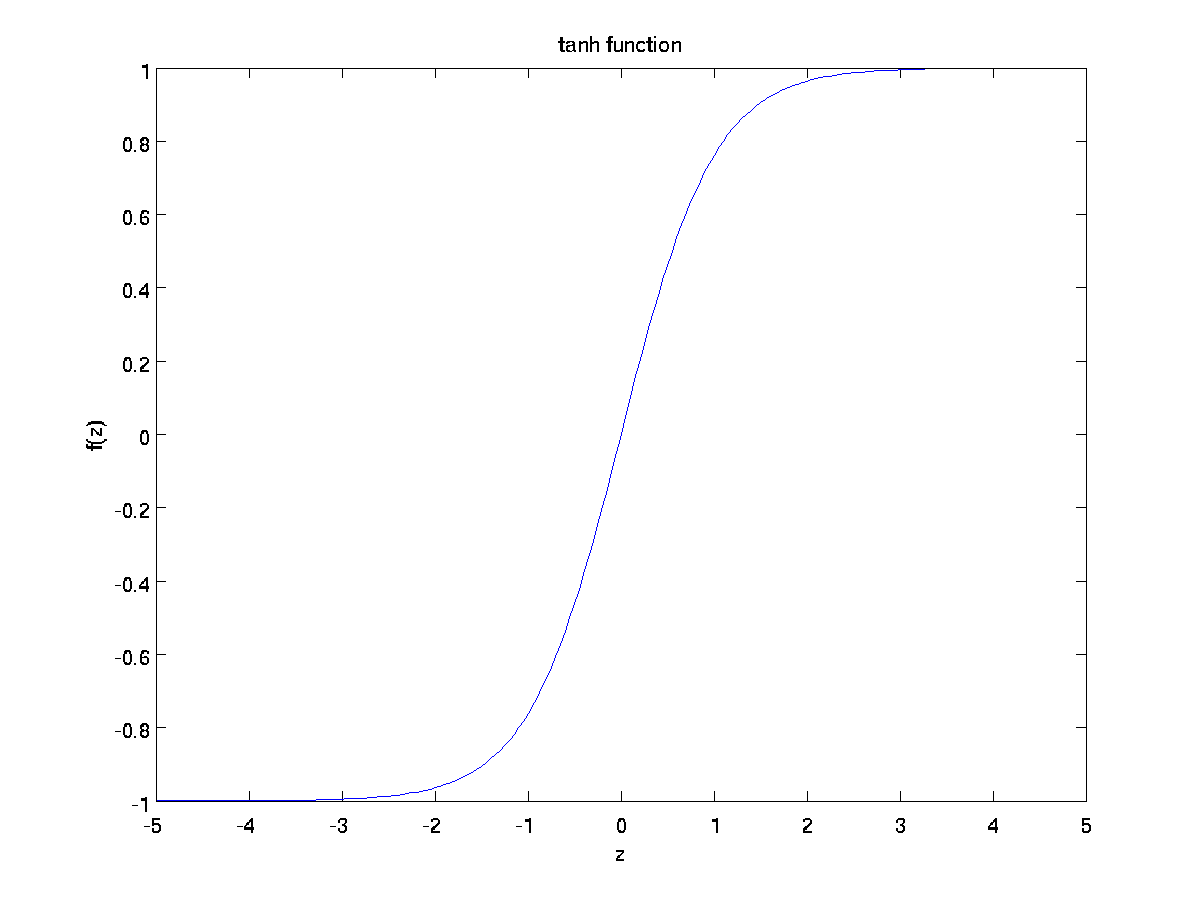
\includegraphics[width=0.45\textwidth]{figures/Tanh_Function.png}
%  %\caption{}\label{fig:step1}
%\end{figure}

\cnt{The $\tanh(z)$ function is a rescaled version of the sigmoid, and its output range is $[ -1,1]$ instead of $[0,1]$.}
    {$\tanh(z)$ 函数是sigmoid函数的一种变体,它的取值范围为 $[-1,1]$,而不是sigmoid函数的 $[0,1]$。}
    {}


\cnt{Note that unlike some other venues (including the OpenClassroom videos, and parts of CS229), we are not using the convention here of $x_0=1$. Instead, the intercept term is handled separately by the parameter $b$.}
    {注意,与其它地方(包括OpenClassroom公开课以及斯坦福大学CS229课程)不同的是,这里我们不再令 $x_0=1$。取而代之,我们用单独的参数 $b$ 来表示截距。}
    {}

\cnt{Finally, one identity that'll be useful later: If $f(z) = 1/(1+\exp(-z))$ is the sigmoid function, then its derivative is given by $f'(z) = f(z) (1-f(z))$. (If $f$ is the $\tanh$ function, then its derivative is given by $f'(z) = 1- (f(z))^2$.) You can derive this yourself using the definition of the sigmoid (or tanh) function.}
    {最后要说明的是,有一个等式我们以后会经常用到:如果选择 $f(z) = 1/(1+\exp(-z))$,也就是sigmoid函数,那么它的导数就是 $f'(z) = f(z) (1-f(z))$ (如果选择 $\tanh$ 函数,那它的导数就是 $f'(z) = 1- (f(z))^2$,你可以根据sigmoid(或tanh)函数的定义自行推导这个等式。}
    {}

\subsubsection{\cnt{Neural Network model}{神经网络模型}{}}

\cnt{A neural network\index{neural network} is put together by hooking together many of our simple ``neurons," so that the output of a neuron can be the input of another. For example, here is a small neural network:}
    {所谓 神经网络\index{神经网络} 就是将许多个单一“神经元”联结在一起,这样,一个“神经元”的输出就可以是另一个“神经元”的输入。例如,下图就是一个简单的神经网络:}
    {}

\begin{figure}[ht] \centering
  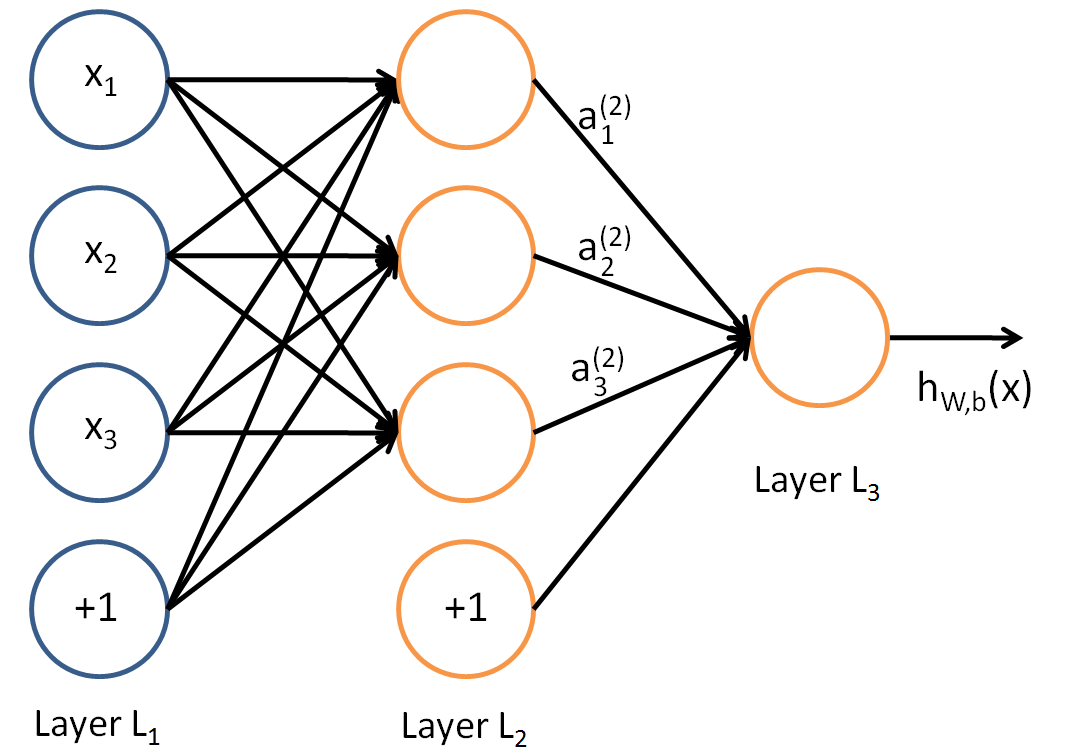
\includegraphics[width=0.6\textwidth]{figures/Network331.png}
  %\caption{}\label{fig:step1}
\end{figure}


\cnt{In this figure, we have used circles to also denote the inputs to the network. The circles labeled ``$+1$" are called \emph{bias units}, and correspond to the intercept term. The leftmost layer of the network is called the \emph{input layer}, and the rightmost layer the \emph{output layer} (which, in this example, has only one node). The middle layer of nodes is called the \emph{hidden layer}, because its values are not observed in the training set. We also say that our example neural network has 3 \emph{input units} (not counting the bias unit), 3 \emph{hidden units}, and 1 \emph{output unit}.}
    {我们使用圆圈来表示神经网络的输入,标上“$+1$”的圆圈被称为\emph{偏置节点},也就是截距项。神经网络最左边的一层叫做\emph{输入层},最右的一层叫做\emph{输出层}(本例中,输出层只有一个节点)。中间所有节点组成的一层叫做\emph{隐藏层},因为我们不能在训练样本集中观测到它们的值。同时可以看到,以上神经网络的例子中有3个输入单元(偏置单元不计在内),3个隐藏单元及一个输出单元。}
    {}


\cnt{We will let ${n}_l$ denote the number of layers in our network; thus $n_l=3$ in our example. We label layer $l$ as $L_l$, so layer $L_1$ is the input layer, and layer $L_{n_l}$ the output layer. Our neural network has parameters $(W,b) = (W^{(1)}, b^{(1)}, W^{(2)}, b^{(2)})$, where we write $W^{(l)}_{ij}$ to denote the parameter (or weight) associated with the connection between unit $j$ in layer $l$, and unit $i$ in layer $l + 1$. (Note the order of the indices.) Also, $b^{(l)}_i$ is the bias associated with unit $i$ in layer $l + 1$. Thus, in our example, we have $W^{(1)} \in \Re^{3\times 3}$, and $W^{(2)} \in \Re^{1\times 3}$. Note that bias units don't have inputs or connections going into them, since they always output the value $+1$. We also let $s_l$ denote the number of nodes in layer $l$ (not counting the bias unit).}
    {我们用 ${n}_l$ 来表示网络的层数,本例中 $n_l=3$,我们将第 $l$ 层记为 $L_l$,于是 $L_1$ 是输入层,输出层是 $L_{n_l}$。本例神经网络有参数 $(W,b) = (W^{(1)}, b^{(1)}, W^{(2)}, b^{(2)})$,其中 $W^{(l)}_{ij}$(下面的式子中用到)是第 $l$ 层第 $j$ 单元与第 $l+1$ 层第 $i$ 单元之间的联接参数(其实就是连接线上的权重,注意标号顺序), $b^{(l)}_i$ 是第 $l+1$ 层第 $i$ 单元的偏置项。因此在本例中, $W^{(1)} \in \Re^{3\times 3}$, $W^{(2)} \in \Re^{1\times 3}$。注意,没有其他单元连向偏置单元(即偏置单元没有输入),因为它们总是输出 $+1$。同时,我们用 $s_l$ 表示第 $l$ 层的节点数(偏置单元不计在内)。}
    {}

\cnt{We will write $a^{(l)}_i$ to denote the \emph{activation} (meaning output value) of unit $i$ in layer $l$. For $l = 1$, we also use $a^{(1)}_i = x_i$ to denote the $i$-th input. Given a fixed setting of the parameters $W,b$, our neural network defines a hypothesis $h_{W,b}(x)$ that outputs a real number. Specifically, the computation that this neural network represents is given by:}
    {我们用 $a^{(l)}_i$ 表示第 $l$ 层第 $i$ 单元的激活值(输出值)。当 $l=1$ 时, $a^{(1)}_i = x_i$,也就是第 $i$ 个输入值(输入值的第 $i$ 个特征)。对于给定参数集合 $W,b$,我们的神经网络就可以按照函数 $h_{W,b}(x)$ 来计算输出结果。本例神经网络的计算步骤如下:}
    {}

\begin{align*}
a_1^{(2)} &= f(W_{11}^{(1)}x_1 + W_{12}^{(1)} x_2 + W_{13}^{(1)} x_3 + b_1^{(1)})  \\
a_2^{(2)} &= f(W_{21}^{(1)}x_1 + W_{22}^{(1)} x_2 + W_{23}^{(1)} x_3 + b_2^{(1)})  \\
a_3^{(2)} &= f(W_{31}^{(1)}x_1 + W_{32}^{(1)} x_2 + W_{33}^{(1)} x_3 + b_3^{(1)})  \\
h_{W,b}(x) &= a_1^{(3)} =  f(W_{11}^{(2)}a_1^{(2)} + W_{12}^{(2)} a_2^{(2)} + W_{13}^{(2)} a_3^{(2)} + b_1^{(2)}) 
\end{align*}

\cnt{In the sequel, we also let $z^{(l)}_i$ denote the total weighted sum of inputs to unit $i$ in layer $l$, including the bias term (e.g., $z_i^{(2)} = \sum_{j=1}^n W^{(1)}_{ij} x_j + b^{(1)}_i)$, so that $a^{(l)}_i = f(z^{(l)}_i)$.}
    {我们用 $z^{(l)}_i$ 表示第 $l$ 层第 $i$ 单元输入加权和(包括偏置单元),比如, $z_i^{(2)} = \sum_{j=1}^n W^{(1)}_{ij} x_j + b^{(1)}_i$,则 $a^{(l)}_i = f(z^{(l)}_i)$。}
    {}


\cnt{Note that this easily lends itself to a more compact notation. Specifically, if we extend the activation function $f(\cdot)$ to apply to vectors in an element-wise fashion (i.e., $f([z_1, z_2, z_3]) = [f(z_1), f(z_2), f(z_3)]$, then we can write the equations above more compactly as:}
    {这样我们就可以得到一种更简洁的表示法。这里我们将激活函数 $f(\cdot)$ 扩展为用向量(分量的形式)来表示,即 $f([z_1, z_2, z_3]) = [f(z_1), f(z_2), f(z_3)]$,那么,上面的等式可以更简洁地表示为:}
    {}

\begin{align*}
z^{(2)} &= W^{(1)} x + b^{(1)} \\
a^{(2)} &= f(z^{(2)}) \\
z^{(3)} &= W^{(2)} a^{(2)} + b^{(2)} \\
h_{W,b}(x) &= a^{(3)} = f(z^{(3)})
\end{align*}

\cnt{We call this step \emph{forward propagation}\index{forward propagation}. More generally, recalling that we also use $a^{(1)} = x$ to also denote the values from the input layer, then given layer $l$'s activations $a^{(l)}$, we can compute layer $l + 1$'s activations $a^{(l+1)}$ as:}
    {我们将上面的计算步骤叫作\emph{前向传播}\index{前向传播}。回想一下,之前我们用 $a^{(1)} = x$ 表示输入层的激活值,那么给定第 $l$ 层的激活值 $a^{(l)}$ 后,第 $l+1$ 层的激活值 $a^{(l+1)}$ 就可以按照下面步骤计算得到:}
    {}

\begin{align*}
z^{(l+1)} &= W^{(l)} a^{(l)} + b^{(l)}   \\
a^{(l+1)} &= f(z^{(l+1)})
\end{align*}

\cnt{By organizing our parameters in matrices and using matrix-vector operations, we can take advantage of fast linear algebra routines to quickly perform calculations in our network.}
    {将参数矩阵化,使用矩阵-向量运算方式,我们就可以利用线性代数的优势对神经网络进行快速求解。}
    {}


\cnt{We have so far focused on one example neural network, but one can also build neural networks with other architectures (meaning patterns of connectivity between neurons), including ones with multiple hidden layers. The most common choice is a $n_l$-layered network where layer $1$ is the input layer, layer $n_l$ is the output layer, and each layer $l$ is densely connected to layer $l+1$. In this setting, to compute the output of the network, we can successively compute all the activations in layer $L_2$, then layer $L_3$, and so on, up to layer $L_{n_l}$, using the equations above that describe the forward propagation step. This is one example of a feedforward neural network, since the connectivity graph does not have any directed loops or cycles.}
    {目前为止,我们讨论了一种神经网络,我们也可以构建另一种结构的神经网络(这里结构指的是神经元之间的联接模式),也就是包含多个隐藏层的神经网络。最常见的一个例子是 $n_l$ 层的神经网络,第 $1$ 层是输入层,第 $n_l$ 层是输出层,中间的每个层 $l$ 与层 $l+1$ 紧密相联。这种模式下,要计算神经网络的输出结果,我们可以按照之前描述的等式,按部就班,进行前向传播,逐一计算第 $L_2$ 层的所有激活值,然后是第 $L_3$ 层的激活值,以此类推,直到第 $L_{n_l}$ 层。这是一个前馈神经网络的例子,因为这种联接图没有闭环或回路。}
    {}


\cnt{Neural networks can also have multiple output units. For example, here is a network with two hidden layers layers $L_2$ and $L_3$ and two output units in layer $L_4$:}
    {神经网络也可以有多个输出单元。比如,下面的神经网络有两层隐藏层: $L_2$ 及 $L_3$,输出层 $L_4$ 有两个输出单元。}
    {}

\begin{figure}[ht] \centering
  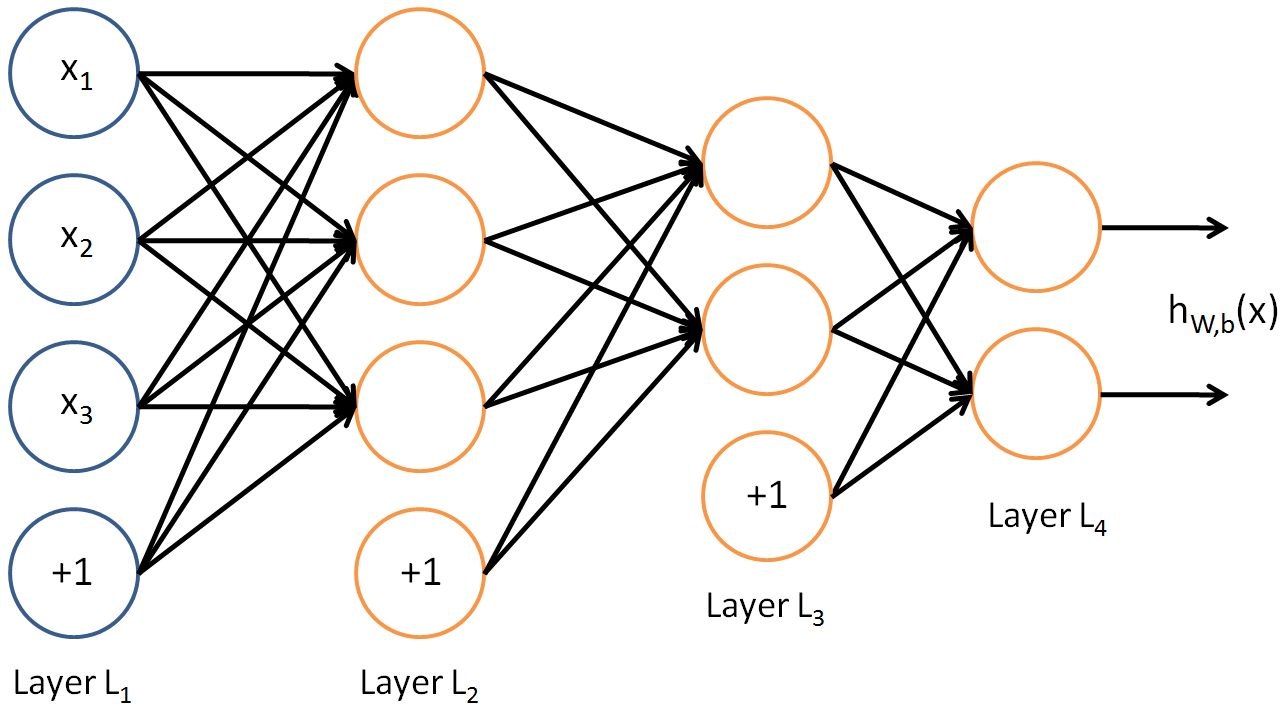
\includegraphics[width=0.7\textwidth]{figures/Network3322.png}
  %\caption{}\label{fig:step1}
\end{figure}

\cnt{To train this network, we would need training examples $(x^{(i)}, y^{(i)})$ where $y^{(i)} \in \Re^2$. This sort of network is useful if there're multiple outputs that you're interested in predicting. (For example, in a medical diagnosis application, the vector $x$ might give the input features of a patient, and the different outputs $y_i$'s might indicate presence or absence of different diseases.)}
    {要求解这样的神经网络,需要样本集 $(x^{(i)}, y^{(i)})$,其中 $y^{(i)} \in \Re^2$。如果你想预测的输出是多个的,那这种神经网络很适用。(比如,在医疗诊断应用中,患者的体征指标就可以作为向量$x$的输入值,而不同的输出值 $y_i$ 可以表示不同的疾病存在与否。)}
    {}


\subsection{\cnt{Backpropagation Algorithm}{反向传导算法}{}} \label{chp:bkpropgationalg}

\cnt{\index{backpropagation}}{\index{反向传导}}{}

\cnt{Suppose we have a fixed training set $\{ (x^{(1)}, y^{(1)}), \ldots, (x^{(m)}, y^{(m)}) \}$ of $m$ training examples. We can train our neural network using batch gradient descent. In detail, for a single training example $(x,y)$, we define the cost function with respect to that single example to be:
}
    {假设我们有一个固定样本集 $\{ (x^{(1)}, y^{(1)}), \ldots, (x^{(m)}, y^{(m)}) \}$,它包含 $m$ 个样例。我们可以用批量梯度下降法来求解神经网络。具体来讲,对于单个样例 $(x,y)$,其代价函数为:}
    {}


\begin{align}
J(W,b; x,y) = \frac{1}{2} \left\| h_{W,b}(x) - y \right\|^2.
\end{align}


\cnt{This is a (one-half) squared-error cost function. Given a training set of $m$ examples, we then define the overall cost function to be:}
    {这是一个(二分之一的)方差代价函数。给定一个包含 $m$ 个样例的数据集,我们可以定义整体代价函数为:}
    {}

 
\begin{align}
J(W,b)
&= \left[ \frac{1}{m} \sum_{i=1}^m J(W,b;x^{(i)},y^{(i)}) \right]
                       + \frac{\lambda}{2} \sum_{l=1}^{n_l-1} \; \sum_{i=1}^{s_l} \; \sum_{j=1}^{s_{l+1}} \left( W^{(l)}_{ji} \right)^2
 \\
&= \left[ \frac{1}{m} \sum_{i=1}^m \left( \frac{1}{2} \left\| h_{W,b}(x^{(i)}) - y^{(i)} \right\|^2 \right) \right]
                       + \frac{\lambda}{2} \sum_{l=1}^{n_l-1} \; \sum_{i=1}^{s_l} \; \sum_{j=1}^{s_{l+1}} \left( W^{(l)}_{ji} \right)^2
\end{align}


\cnt{The first term in the definition of J(W,b) is an average sum-of-squares error term. The second term is a regularization term (also called a \emph{weight decay} term) that tends to decrease the magnitude of the weights, and helps prevent overfitting.}
    {以上公式中的第一项 $J(W,b)$ 是一个均方差项。第二项是一个规则化项(也叫\emph{权重衰减项}),其目的是减小权重的幅度,防止过度拟合。}
    {}
\footnote{\cnt{Usually weight decay is not applied to the bias terms $b^{(l)}_i$, as reflected in our definition for $J(W,b)$. Applying weight decay to the bias units usually makes only a small difference to the final network, however. If you've taken CS229 (Machine Learning) at Stanford or watched the course's videos on YouTube, you may also recognize this weight decay as essentially a variant of the Bayesian regularization method you saw there, where we placed a Gaussian prior on the parameters and did MAP (instead of maximum likelihood) estimation.}{通常权重衰减的计算并不使用偏置项 $b^{(l)}_i$,比如我们在 $J(W, b)$ 的定义中就没有使用。一般来说,将偏置项包含在权重衰减项中只会对最终的神经网络产生很小的影响。如果你在斯坦福选修过CS229(机器学习)课程,或者在YouTube上看过课程视频,你会发现这个权重衰减实际上是课上提到的贝叶斯规则化方法的变种。在贝叶斯规则化方法中,我们将高斯先验概率引入到参数中计算MAP(极大后验)估计(而不是极大似然估计)。}{}}

\cnt{The \emph{weight decay parameter} $\lambda$ controls the relative importance of the two terms. Note also the slightly overloaded notation: $J(W,b;x,y)$ is the squared error cost with respect to a single example; $J(W,b)$ is the overall cost function, which includes the weight decay term.}
    {\emph{权重衰减参数} $\lambda$ 用于控制公式中两项的相对重要性。在此重申一下这两个复杂函数的含义:$J(W,b;x,y)$ 是针对单个样例计算得到的方差代价函数;$J(W,b)$ 是整体样本代价函数,它包含权重衰减项。}
    {}


\cnt{This cost function above is often used both for classification and for regression problems. For classification, we let $y = 0$ or $1$ represent the two class labels (recall that the sigmoid activation function outputs values in $[0,1]$; if we were using a tanh activation function, we would instead use $-1$ and $+1$ to denote the labels). For regression problems, we first scale our outputs to ensure that they lie in the $[0,1]$ range (or if we were using a tanh activation function, then the $[-1,1]$ range).}
    {以上的代价函数经常被用于分类和回归问题。在分类问题中,我们用 $y = 0$ 或 $1$,来代表两种类型的标签(回想一下,这是因为 sigmoid激活函数的值域为 $[0,1]$;如果我们使用双曲正切型激活函数,那么应该选用 $-1$ 和 $+1$ 作为标签)。对于回归问题,我们首先要变换输出值域(译者注:也就是 $y$),以保证其范围为 $[0,1]$ (同样地,如果我们使用双曲正切型激活函数,要使输出值域为 $[-1,1]$)。}
    {}

\cnt{Our goal is to minimize $J(W,b)$ as a function of $W$ and $b$. To train our neural network, we will initialize each parameter $W^{(l)}_{ij}$ and each $b^{(l)}_i$ to a small random value near zero (say according to a ${Normal}(0,\epsilon^2)$ distribution for some small $\epsilon$, say $0.01$), and then apply an optimization algorithm such as batch gradient descent. Since $J(W,b)$ is a non-convex function, gradient descent is susceptible to local optima; however, in practice gradient descent usually works fairly well. Finally, note that it is important to initialize the parameters randomly, rather than to all $0$'s. If all the parameters start off at identical values, then all the hidden layer units will end up learning the same function of the input (more formally, $W^{(1)}_{ij}$ will be the same for all values of $i$, so that $a^{(2)}_1 = a^{(2)}_2 = a^{(2)}_3 = \ldots$ for any input $x$). The random initialization serves the purpose of \emph{symmetry breaking}.}
    {我们的目标是针对参数 $W$ 和 $b$ 来求其函数 $J(W,b)$ 的最小值。为了求解神经网络,我们需要将每一个参数 $W^{(l)}_{ij}$ 和 $b^{(l)}_i$ 初始化为一个很小的、接近零的随机值(比如说,使用正态分布 ${Normal}(0,\epsilon^2)$ 生成的随机值,其中 $\epsilon$ 设置为 $0.01$ ),之后对目标函数使用诸如批量梯度下降法的最优化算法。因为 $J(W, b)$ 是一个非凸函数,梯度下降法很可能会收敛到局部最优解;但是在实际应用中,梯度下降法通常能得到令人满意的结果。最后,需要再次强调的是,要将参数进行随机初始化,而不是全部置为 $0$。如果所有参数都用相同的值作为初始值,那么所有隐藏层单元最终会得到与输入值有关的、相同的函数(也就是说,对于所有 $i$,$W^{(1)}_{ij}$ 都会取相同的值,那么对于任何输入 $x$ 都会有:$a^{(2)}_1 = a^{(2)}_2 = a^{(2)}_3 = \ldots$ )。随机初始化的目的是使\emph{对称失效}。}
    {}


\cnt{One iteration of gradient descent updates the parameters $W,b$ as follows:}
    {梯度下降法中每一次迭代都按照如下公式对参数 $W$ 和 $b$ 进行更新:}
    {}

\begin{align}
W_{ij}^{(l)} &= W_{ij}^{(l)} - \alpha \frac{\partial}{\partial W_{ij}^{(l)}} J(W,b) \\
b_{i}^{(l)} &= b_{i}^{(l)} - \alpha \frac{\partial}{\partial b_{i}^{(l)}} J(W,b)
\end{align}


\cnt{where $\alpha$ is the learning rate. The key step is computing the partial derivatives above. We will now describe the \emph{backpropagation algorithm}, which gives an efficient way to compute these partial derivatives.}
    {其中 $\alpha$ 是学习速率。其中关键步骤是计算偏导数。我们现在来讲一下\emph{反向传播算法},它是计算偏导数的一种有效方法。}
    {}


\cnt{We will first describe how backpropagation can be used to compute $\frac{\partial}{\partial W_{ij}^{(l)}} J(W,b; x, y)$ and $\frac{\partial}{\partial b_{i}^{(l)}} J(W,b; x, y)$, the partial derivatives of the cost function $J(W,b;x,y)$ defined with respect to a single example $(x,y)$. Once we can compute these, we see that the derivative of the overall cost function $J(W,b)$ can be computed as:}
    {我们首先来讲一下如何使用反向传播算法来计算 $\frac{\partial}{\partial W_{ij}^{(l)}} J(W,b; x, y)$ 和 $\frac{\partial}{\partial b_{i}^{(l)}} J(W,b; x, y)$,这两项是单个样例 $(x,y)$ 的代价函数 $J(W,b;x,y)$ 的偏导数。一旦我们求出该偏导数,就可以推导出整体代价函数 $J(W,b)$ 的偏导数:}
    {}


\begin{align}
\frac{\partial}{\partial W_{ij}^{(l)}} J(W,b) &=
\left[ \frac{1}{m} \sum_{i=1}^m \frac{\partial}{\partial W_{ij}^{(l)}} J(W,b; x^{(i)}, y^{(i)}) \right] + \lambda W_{ij}^{(l)} \\
\frac{\partial}{\partial b_{i}^{(l)}} J(W,b) &=
\frac{1}{m}\sum_{i=1}^m \frac{\partial}{\partial b_{i}^{(l)}} J(W,b; x^{(i)}, y^{(i)})
\end{align}

\cnt{The two lines above differ slightly because weight decay is applied to $W$ but not $b$.}
    {以上两行公式稍有不同,第一行比第二行多出一项,是因为权重衰减是作用于 $W$ 而不是 $b$。}
    {}


\cnt{The intuition behind the backpropagation algorithm is as follows. Given a training example $(x,y)$, we will first run a ``forward pass" to compute all the activations throughout the network, including the output value of the hypothesis $h_{W,b}(x)$. Then, for each node $i$ in layer $l$, we would like to compute an ``error term" $\delta^{(l)}_i$ that measures how much that node was ``responsible" for any errors in our output. For an output node, we can directly measure the difference between the network's activation and the true target value, and use that to define $\delta^{(n_l)}_i$ (where layer $n_l$ is the output layer). How about hidden units? For those, we will compute $\delta^{(l)}_i$ based on a weighted average of the error terms of the nodes that uses $a^{(l)}_i$ as an input. In detail, here is the backpropagation algorithm:}
    {反向传播算法的思路如下:给定一个样例 $(x,y)$,我们首先进行“前向传导”运算,计算出网络中所有的激活值,包括 $h_{W,b}(x)$ 的输出值。之后,针对第 $l$ 层的每一个节点 $i$,我们计算出其“残差” $\delta^{(l)}_i$,该残差表明了该节点对最终输出值的残差产生了多少影响。对于最终的输出节点,我们可以直接算出网络产生的激活值与实际值之间的差距,我们将这个差距定义为 $\delta^{(n_l)}_i$ (第 $n_l$ 层表示输出层)。对于隐藏单元我们如何处理呢?我们将基于节点(译者注:第 $l+1$ 层节点)残差的加权平均值计算 $\delta^{(l)}_i$,这些节点以 $a^{(l)}_i$ 作为输入。下面将给出反向传导算法的细节:}
    {}

\begin{enumerate}
  \item
\cnt{Perform a feedforward pass, computing the activations for layers $L_2, L_3, \ldots$, and so on up to the output layer $L_{n_l}$.}
    {进行前馈传导计算,利用前向传导公式,得到 $L_2, L_3, \ldots$ 直到输出层 $L_{n_l}$ 的激活值。}
    {}

  \item
\cnt{For each output unit $i$ in layer $n_l$ (the output layer), set}
    {对于第 $n_l$ 层(输出层)的每个输出单元 $i$,我们根据以下公式计算残差:}
    {}

\begin{align}
\delta^{(n_l)}_i
= \frac{\partial}{\partial z^{(n_l)}_i} \;\;
        \frac{1}{2} \left\|y - h_{W,b}(x)\right\|^2 = - (y_i - a^{(n_l)}_i) \cdot f'(z^{(n_l)}_i)
\end{align}
\footnote{译者注:

\begin{align}
\delta^{(n_l)}_i &= \frac{\partial}{\partial z^{n_l}_i}J(W,b;x,y)
 = \frac{\partial}{\partial z^{n_l}_i}\frac{1}{2} \left\|y - h_{W,b}(x)\right\|^2 \\
 &= \frac{\partial}{\partial z^{n_l}_i}\frac{1}{2} \sum_{j=1}^{S_{n_l}} (y_j-a_j^{(n_l)})^2
 = \frac{\partial}{\partial z^{n_l}_i}\frac{1}{2} \sum_{j=1}^{S_{n_l}} (y_j-f(z_j^{(n_l)}))^2 \\
 &= - (y_i - f(z_i^{(n_l)})) \cdot f'(z^{(n_l)}_i)
 = - (y_i - a^{(n_l)}_i) \cdot f'(z^{(n_l)}_i)
\end{align}
}

  \item
\cnt{For $l = n_l-1, n_l-2, n_l-3, \ldots, 2$}
    {对 $l = n_l-1, n_l-2, n_l-3, \ldots, 2$ 的各个层,}
    {}

\cnt{For each node $i$ in layer $l$, set}
    {计算第 $l$ 层的第 $i$ 个节点的残差:}
    {}
$$
\delta^{(l)}_i = \left( \sum_{j=1}^{s_{l+1}} W^{(l)}_{ji} \delta^{(l+1)}_j \right) f'(z^{(l)}_i)
$$
\footnote{译者注:
 
\begin{align}
\delta^{(n_l-1)}_i &=\frac{\partial}{\partial z^{n_l-1}_i}J(W,b;x,y)
 = \frac{\partial}{\partial z^{n_l-1}_i}\frac{1}{2} \left\|y - h_{W,b}(x)\right\|^2 
 = \frac{\partial}{\partial z^{n_l-1}_i}\frac{1}{2} \sum_{j=1}^{S_{n_l}}(y_j-a_j^{(n_l)})^2 \\
&= \frac{1}{2} \sum_{j=1}^{S_{n_l}}\frac{\partial}{\partial z^{n_l-1}_i}(y_j-a_j^{(n_l)})^2
 = \frac{1}{2} \sum_{j=1}^{S_{n_l}}\frac{\partial}{\partial z^{n_l-1}_i}(y_j-f(z_j^{(n_l)}))^2 \\
&= \sum_{j=1}^{S_{n_l}}-(y_j-f(z_j^{(n_l)})) \cdot \frac{\partial}{\partial z_i^{(n_l-1)}}f(z_j^{(n_l)})
 = \sum_{j=1}^{S_{n_l}}-(y_j-f(z_j^{(n_l)})) \cdot  f'(z_j^{(n_l)}) \cdot \frac{\partial z_j^{(n_l)}}{\partial z_i^{(n_l-1)}} \\
&= \sum_{j=1}^{S_{n_l}} \delta_j^{(n_l)} \cdot \frac{\partial z_j^{(n_l)}}{\partial z_i^{n_l-1}}
 = \sum_{j=1}^{S_{n_l}} \left(\delta_j^{(n_l)} \cdot \frac{\partial}{\partial z_i^{n_l-1}}\sum_{k=1}^{S_{n_l-1}}f(z_k^{n_l-1}) \cdot W_{jk}^{n_l-1}\right) \\
&= \sum_{j=1}^{S_{n_l}} \delta_j^{(n_l)} \cdot  W_{ji}^{n_l-1} \cdot f'(z_i^{n_l-1})
 = \left(\sum_{j=1}^{S_{n_l}}W_{ji}^{n_l-1}\delta_j^{(n_l)}\right)f'(z_i^{n_l-1})
\end{align}

将上式中的 $n_l-1$ 与 $n_l$ 的关系替换为 $l$ 与 $l+1$ 的关系,就可以得到:
$$\delta^{(l)}_i = \left( \sum_{j=1}^{s_{l+1}} W^{(l)}_{ji} \delta^{(l+1)}_j \right) f'(z^{(l)}_i)$$
以上逐次从后向前求导的过程即为“反向传导”的本意所在。
}

  \item
\cnt{Compute the desired partial derivatives, which are given as:}
    {计算我们需要的偏导数,计算方法如下:}
    {}

\begin{align}
\frac{\partial}{\partial W_{ij}^{(l)}} J(W,b; x, y) &= a^{(l)}_j \delta_i^{(l+1)} \\
\frac{\partial}{\partial b_{i}^{(l)}} J(W,b; x, y) &= \delta_i^{(l+1)}.
\end{align}

\end{enumerate}

\cnt{Finally, we can also re-write the algorithm using matrix-vectorial notation. We will use ``$\bullet$" to denote the element-wise product operator (denoted ``\texttt{.*}" in Matlab or Octave, and also called the Hadamard product), so that if $a = b \bullet c$, then $a_i = b_ic_i$. Similar to how we extended the definition of $f(\cdot)$ to apply element-wise to vectors, we also do the same for $f'(\cdot)$ (so that $f'([z_1, z_2, z_3]) =[f'(z_1),f'(z_2),f'(z_3)]$ ).}
    {最后,我们用矩阵-向量表示法重写以上算法。我们使用“$\bullet$” 表示向量乘积运算符(在Matlab或Octave里用“\texttt{.*}”表示,也称作阿达马乘积)。若 $a = b \bullet c$,则 $a_i = b_ic_i$。在上一个教程中我们扩展了 $f(\cdot)$ 的定义,使其包含向量运算,这里我们也对偏导数 $f'(\cdot)$ 也做了同样的处理(于是又有  $f'([z_1, z_2, z_3]) = [f'(z_1), f'(z_2), f'(z_3)]$)。}
    {}


\cnt{The algorithm can then be written:}
    {那么,反向传播算法可表示为以下几个步骤:}
    {}

\begin{enumerate}
  \item
\cnt{Perform a feedforward pass, computing the activations for layers $L_2$, $L_3$, up to the output layer $L_{n_l}$, using the equations defining the forward propagation steps}
    {进行前馈传导计算,利用前向传导公式,得到 $L_2, L_3, \ldots$ 直到输出层 $L_{n_l}$ 的激活值。}
    {}

  \item
\cnt{For the output layer (layer $n_l$), set}
    {对输出层(第 $n_l$ 层),计算:}
    {}

\begin{align}
\delta^{(n_l)}
= - (y - a^{(n_l)}) \bullet f'(z^{(n_l)})
\end{align}

  \item
\cnt{For $l = n_l-1, n_l-2, n_l-3, \ldots, 2$, Set}
    {对于 $l = n_l-1, n_l-2, n_l-3, \ldots, 2$ 的各层,计算:}
    {}

\begin{align}
\delta^{(l)} = \left((W^{(l)})^T \delta^{(l+1)}\right) \bullet f'(z^{(l)})
\end{align}

  \item
\cnt{Compute the desired partial derivatives:}
    {计算最终需要的偏导数值:}
    {}

\begin{align}
\nabla_{W^{(l)}} J(W,b;x,y) &= \delta^{(l+1)} (a^{(l)})^T, \\
\nabla_{b^{(l)}} J(W,b;x,y) &= \delta^{(l+1)}.
\end{align}

\end{enumerate}

\cnt{\emph{Implementation note}: In steps 2 and 3 above, we need to compute $f'(z^{(l)}_i)$ for each value of $i$. Assuming $f(z)$ is the sigmoid activation function, we would already have $a^{(l)}_i$ stored away from the forward pass through the network. Thus, using the expression that we worked out earlier for $f'(z)$, we can compute this as $f'(z^{(l)}_i) = a^{(l)}_i (1- a^{(l)}_i)$.}
    {\emph{实现中应注意}:在以上的第2步和第3步中,我们需要为每一个 $i$ 值计算其 $f'(z^{(l)}_i$)。假设 $f(z)$ 是sigmoid函数,并且我们已经在前向传导运算中得到了 $a^{(l)}_i$。那么,使用我们早先推导出的 $f'(z)$ 表达式,就可以计算得到 $f'(z^{(l)}_i) = a^{(l)}_i (1- a^{(l)}_i)$。}
    {}

\cnt{Finally, we are ready to describe the full gradient descent algorithm. In the pseudo-code below, $\Delta W^{(l)}$ is a matrix (of the same dimension as $W^{(l)}$), and $\Delta b^{(l)}$ is a vector (of the same dimension as $b^{(l)}$). Note that in this notation, ``$\Delta W^{(l)}$" is a matrix, and in particular it isn't ``$\Delta$ times $W^{(l)}$." We implement one iteration of batch gradient descent as follows:}
    {最后,我们将对梯度下降算法做个全面总结。在下面的伪代码中,$\Delta W^{(l)}$ 是一个与矩阵 $W^{(l)}$ 维度相同的矩阵,$\Delta b^{(l)}$ 是一个与 $b^{(l)}$ 维度相同的向量。注意这里“$\Delta W^{(l)}$”是一个矩阵,而不是“$\Delta$ 与 $W^{(l)}$ 相乘”。下面,我们实现批量梯度下降法中的一次迭代:}
    {}

\begin{enumerate}
  \item
\cnt{Set $\Delta W^{(l)} := 0$, $\Delta b^{(l)} := 0$ (matrix/vector of zeros) for all $l$.}
    {对于所有 $l$,令 $\Delta W^{(l)} := 0$, $\Delta b^{(l)} := 0$ (设置为全零矩阵或全零向量)}
    {}

  \item
\cnt{or $i = 1$ to $m$,}
    {对于 $i = 1$ 到 $m$,}
    {}
    \begin{enumerate}
      \item
\cnt{Use backpropagation to compute $\nabla_{W^{(l)}} J(W,b;x,y)$ and $\nabla_{b^{(l)}} J(W,b;x,y)$.}
    {使用反向传播算法计算 $\nabla_{W^{(l)}} J(W,b;x,y)$ 和 $\nabla_{b^{(l)}} J(W,b;x,y)$。}
    {}
      \item
\cnt{Set $\Delta W^{(l)} := \Delta W^{(l)} + \nabla_{W^{(l)}} J(W,b;x,y)$.}
    {计算 $\Delta W^{(l)} := \Delta W^{(l)} + \nabla_{W^{(l)}} J(W,b;x,y)$。}
    {}
      \item
\cnt{Set $\Delta b^{(l)} := \Delta b^{(l)} + \nabla_{b^{(l)}} J(W,b;x,y)$.}
    {计算 $\Delta b^{(l)} := \Delta b^{(l)} + \nabla_{b^{(l)}} J(W,b;x,y)$。}
    {}
    \end{enumerate}

  \item
\cnt{Update the parameters:}
    {更新权重参数:}
    {}

 \begin{align}
W^{(l)} &= W^{(l)} - \alpha \left[ \left(\frac{1}{m} \Delta W^{(l)} \right) + \lambda W^{(l)}\right] \\
b^{(l)} &= b^{(l)} - \alpha \left[\frac{1}{m} \Delta b^{(l)}\right]
\end{align}

\end{enumerate}

\cnt{To train our neural network, we can now repeatedly take steps of gradient descent to reduce our cost function $J(W,b)$.}
    {现在,我们可以重复梯度下降法的迭代步骤来减小代价函数 $J(W,b)$ 的值,进而求解我们的神经网络。}
    {}


\subsection{\cnt{Gradient checking and advanced optimization}{梯度检验与高级优化}{}} \label{chp:gradcheckingopt}

\cnt{Backpropagation is a notoriously difficult algorithm to debug and get right, especially since many subtly buggy implementations of it -- for example, one that has an off-by-one error in the indices and that thus only trains some of the layers of weights, or an implementation that omits the bias term -- will manage to learn something that can look surprisingly reasonable (while performing less well than a correct implementation). Thus, even with a buggy implementation, it may not at all be apparent that anything is amiss. In this section, we describe a method for numerically checking the derivatives computed by your code to make sure that your implementation is correct. Carrying out the derivative checking procedure described here will significantly increase your confidence in the correctness of your code.}
    {众所周知,反向传播算法很难调试得到正确结果,尤其是当实现程序存在很多难于发现的bug时。举例来说,索引的缺位错误(off-by-one error)会导致只有部分层的权重得到训练,再比如忘记计算偏置项。这些错误会使你得到一个看似十分合理的结果(但实际上比正确代码的结果要差)。因此,但从计算结果上来看,我们很难发现代码中有什么东西遗漏了。本节中,我们将介绍一种对求导结果进行数值检验的方法,该方法可以验证求导代码是否正确。另外,使用本节所述求导检验方法,可以帮助你提升写正确代码的信心。}
    {}
\cnt{}
    {\footnote{缺位错误(Off-by-one error)举例说明:比如 $for$ 循环中循环 $m$ 次,正确应该是 $for (i=1;~i<=m;~i++)$,但有时程序员疏忽,会写成 $for (i=1;~i<m;~i++)$,这就是缺位错误。}}
    {}

\cnt{Suppose we want to minimize $J(\theta)$ as a function of $\theta$. For this example, suppose $J : \Re \mapsto \Re$, so that $\theta \in \Re$. In this 1-dimensional case, one iteration of gradient descent is given by}
    {假设我们想要最小化以 $\theta$ 为自变量的目标函数 $J(\theta)$。假设 $J : \Re \mapsto \Re$,则 $\theta \in \Re$。在一维的情况下,一次迭代的梯度下降公式是}
    {}

\begin{align}
\theta := \theta - \alpha \frac{d}{d\theta}J(\theta).
\end{align}

\cnt{Suppose also that we have implemented some function $g(\theta)$ that purportedly computes $\frac{d}{d\theta}J(\theta)$, so that we implement gradient descent using the update $\theta := \theta - \alpha g(\theta)$. How can we check if our implementation of $g$ is correct?}
    {再假设我们已经用代码实现了计算 $\frac{d}{d\theta}J(\theta)$ 的函数 $g(\theta)$,接着我们使用 $\theta := \theta - \alpha g(\theta)$ 来实现梯度下降算法。那么我们如何检验 $g$ 的实现是否正确呢?}
    {}

\cnt{Recall the mathematical definition of the derivative as}
    {回忆导数的数学定义:}
    {}

\begin{align}
\frac{d}{d\theta}J(\theta) = \lim_{\epsilon \rightarrow 0}
\frac{J(\theta+ \epsilon) - J(\theta-\epsilon)}{2 \epsilon}.
\end{align}

\cnt{Thus, at any specific value of $\theta$, we can numerically approximate the derivative as follows:}
    {那么对于任意 $\theta$ 值,我们都可以对等式左边的导数用:}
    {}

\begin{align}
\frac{J(\theta+{\rm EPSILON}) - J(\theta-{\rm EPSILON})}{2 \times {\rm EPSILON}}
\end{align}

\cnt{}
    {来近似。}
    {}


\cnt{In practice, we set EPSILON to a small constant, say around $10^{-4}$. (There's a large range of values of EPSILON that should work well, but we don't set EPSILON to be ``extremely" small, say $10^{-20}$, as that would lead to numerical roundoff errors.)}
    {实际应用中,我们常将 $EPSILON$ 设为一个很小的常量,比如在 $10^{-4}$ 数量级(虽然 $EPSILON$ 的取值范围可以很大,但是我们不会将它设得太小,比如 $10^{-20}$,因为那将导致数值舍入误差。)}
    {}

\cnt{Thus, given a function $g(\theta)$ that is supposedly computing $\frac{d}{d\theta}J(\theta)$, we can now numerically verify its correctness by checking that}
    {给定一个被认为能计算 $\frac{d}{d\theta}J(\theta)$ 的函数 $g(\theta)$,我们可以用下面的数值检验公式}
    {}

\begin{align}
g(\theta) \approx
\frac{J(\theta+{\rm EPSILON}) - J(\theta-{\rm EPSILON})}{2 \times {\rm EPSILON}}.
\end{align}

\cnt{}
    {计算两端是否一样来检验函数是否正确。}
    {}


\cnt{The degree to which these two values should approximate each other will depend on the details of $J$. But assuming ${\rm EPSILON} = 10^{-4}$, you'll usually find that the left- and right-hand sides of the above will agree to at least 4 significant digits (and often many more).}
    {上式两端值的接近程度取决于 $J$ 的具体形式。但是在假定 ${\rm EPSILON} = 10^{-4}$ 的情况下,你通常会发现上式左右两端至少有4位有效数字是一样的(通常会更多)。}
    {}


\cnt{Now, consider the case where $\theta \in \Re^n$ is a vector rather than a single real number (so that we have $n$ parameters that we want to learn), and $J: \Re^n \mapsto \Re$. In our neural network example we used ``$J(W,b)$," but one can imagine ``unrolling" the parameters $W,b$ into a long vector $\theta$. We now generalize our derivative checking procedure to the case where $\theta$ may be a vector.}
    {现在,考虑 $\theta \in \Re^n$ 是一个向量而非一个实数(那么就有 $n$ 个参数要学习得到),并且 $J: \Re^n \mapsto \Re$。在神经网络的例子里我们使用 $J(W,b)$,可以想象为把参数 $W,b$ 组合扩展成一个长向量 $\theta$。现在我们将求导检验方法推广到一般化,即 $\theta$ 是一个向量的情况。}
    {}

\cnt{Suppose we have a function $g_i(\theta)$ that purportedly computes $\frac{\partial}{\partial \theta_i} J(\theta)$; we'd like to check if $g_i$ is outputting correct derivative values. Let $\theta^{(i+)} = \theta + {\rm EPSILON} \times \vec{e}_i$, where}
    {假设我们有一个用于计算 $\frac{\partial}{\partial \theta_i} J(\theta)$ 的函数 $g_i(\theta)$;我们想要检验 $g_i$ 是否输出正确的求导结果。我们定义 $\theta^{(i+)} = \theta + {\rm EPSILON} \times \vec{e}_i$,其中}
    {}
\begin{align}
\vec{e}_i = \begin{bmatrix}0 \\ 0 \\ \vdots \\ 1 \\ \vdots \\ 0\end{bmatrix}
\end{align}
\cnt{is the $i$-th basis vector (a vector of the same dimension as $\theta$, with a ``1" in the $i$-th position and ``0"s everywhere else). So, $\theta^{(i+)}$ is the same as $\theta$, except its $i$-th element has been incremented by EPSILON. Similarly, let $\theta^{(i-)} = \theta - {\rm EPSILON} \times \vec{e}_i$ be the corresponding vector with the $i$-th element decreased by EPSILON. We can now numerically verify $g_i(\theta)$'s correctness by checking, for each $i$, that:}
    {是第 $i$ 个基向量(维度和 $\theta$ 相同,在第 $i$ 行是“$1$”而其他行是“$0$”)。所以,$\theta^{(i+)}$ 和 $\theta$ 几乎相同,除了第 $i$ 行元素增加了 $EPSILON$。类似地,$\theta^{(i-)} = \theta - {\rm EPSILON} \times \vec{e}_i$ 得到的第 $i$ 行减小了 $EPSILON$。然后我们可以对每个 $i$ 检查下式是否成立,进而验证 $g_i(\theta)$ 的正确性:}
    {}

\begin{align}
g_i(\theta) \approx
\frac{J(\theta^{(i+)}) - J(\theta^{(i-)})}{2 \times {\rm EPSILON}}.
\end{align}

\cnt{When implementing backpropagation to train a neural network, in a correct implementation we will have that}
    {当用反射传播算法求解神经网络时,正确算法实现会得到:}
    {}

\begin{align}
\nabla_{W^{(l)}} J(W,b) &= \left( \frac{1}{m} \Delta W^{(l)} \right) + \lambda W^{(l)} \\
\nabla_{b^{(l)}} J(W,b) &= \frac{1}{m} \Delta b^{(l)}.
\end{align}

\cnt{This result shows that the final block of psuedo-code in Backpropagation Algorithm \ref{chp:bkpropgationalg} is indeed implementing gradient descent. To make sure your implementation of gradient descent is correct, it is usually very helpful to use the method described above to numerically compute the derivatives of $J(W,b)$, and thereby verify that your computations of $\left(\frac{1}{m}\Delta W^{(l)} \right) + \lambda W$ and $\frac{1}{m}\Delta b^{(l)}$ are indeed giving the derivatives you want.}
    {以上结果与反向传播算法(\ref{chp:bkpropgationalg})中的最后一段伪代码一致,都是计算梯度下降。为了验证梯度下降代码的正确性,使用上述数值检验方法计算 $J(W,b)$ 的导数,然后验证 $\left(\frac{1}{m}\Delta W^{(l)} \right) + \lambda W$ 与 $\frac{1}{m}\Delta b^{(l)}$ 是否能够给出正确的求导结果。}
    {}

\cnt{Finally, so far our discussion has centered on using gradient descent to minimize $J(\theta)$. If you have implemented a function that computes $J(\theta)$ and $\nabla_\theta J(\theta)$, it turns out there are more sophisticated algorithms than gradient descent for trying to minimize $J(\theta)$. For example, one can envision an algorithm that uses gradient descent, but automatically tunes the learning rate $\alpha$ so as to try to use a step-size that causes $\theta$ to approach a local optimum as quickly as possible. There are other algorithms that are even more sophisticated than this; for example, there are algorithms that try to find an approximation to the Hessian matrix, so that it can take more rapid steps towards a local optimum (similar to Newton's method). A full discussion of these algorithms is beyond the scope of these notes, but one example is the L-BFGS algorithm. (Another example is the conjugate gradient algorithm.) You will use one of these algorithms in the programming exercise. The main thing you need to provide to these advanced optimization algorithms is that for any $\theta$, you have to be able to compute $J(\theta)$ and $\nabla_\theta J(\theta)$. These optimization algorithms will then do their own internal tuning of the learning rate/step-size $\alpha$ (and compute its own approximation to the Hessian, etc.) to automatically search for a value of $\theta$ that minimizes $J(\theta)$. Algorithms such as L-BFGS and conjugate gradient can often be much faster than gradient descent.}
    {迄今为止,我们的讨论都集中在使用梯度下降法来最小化 $J(\theta)$。如果你已经实现了一个计算 $J(\theta)$ 和 $\nabla_\theta J(\theta)$ 的函数,那么其实还有更精妙的算法来最小化 $J(\theta)$。举例来说,可以想象这样一个算法:它使用梯度下降,并能够自动调整学习速率 $\alpha$,以得到合适的步长值,最终使 $\theta$ 能够快速收敛到一个局部最优解。还有更妙的算法:比如可以寻找一个Hessian矩阵的近似,得到最佳步长值,使用该步长值能够更快地收敛到局部最优(和牛顿法类似)。此类算法的详细讨论已超出了这份讲义的范围,但是L-BFGS算法我们以后会有论述(另一个例子是共轭梯度算法)。你将在编程练习里使用这些算法中的一个。使用这些高级优化算法时,你需要提供关键的函数:即对于任一个 $\theta$,需要你计算出 $J(\theta)$ 和 $\nabla_\theta J(\theta)$。之后,这些优化算法会自动调整学习速率/步长值 $\alpha$ 的大小(并计算Hessian近似矩阵等等)来自动寻找 $J(\theta)$ 最小化时 $\theta$ 的值。诸如L-BFGS和共轭梯度算法通常比梯度下降法快很多。}
    {}

\subsection{\cnt{Autoencoders and Sparsity}{自编码算法与稀疏性}{}} \label{chp:autoencsparse}

\cnt{So far, we have described the application of neural networks to supervised learning, in which we have labeled training examples. Now suppose we have only a set of unlabeled training examples $\{x^{(1)}, x^{(2)}, x^{(3)}, \ldots\}$, where $x^{(i)} \in \Re^{n}$. An autoencoder neural network is an unsupervised learning algorithm that applies backpropagation, setting the target values to be equal to the inputs. I.e., it uses $y^{(i)} = x^{(i)}$.}
    {目前为止,我们已经讨论了神经网络在有监督学习中的应用。在有监督学习中,训练样本是有类别标签的。现在假设我们只有一个没有带类别标签的训练样本集合 $\{x^{(1)}, x^{(2)}, x^{(3)}, \ldots\}$,其中 $x^{(i)} \in \Re^{n}$。自编码神经网络是一种无监督学习算法,它使用了反向传播算法,并让目标值等于输入值,比如 $y^{(i)} = x^{(i)}$。}
    {}

\cnt{Here is an autoencoder:}
    {下图是一个自编码神经网络的示例。 }
    {}

\begin{figure}[ht] \centering
  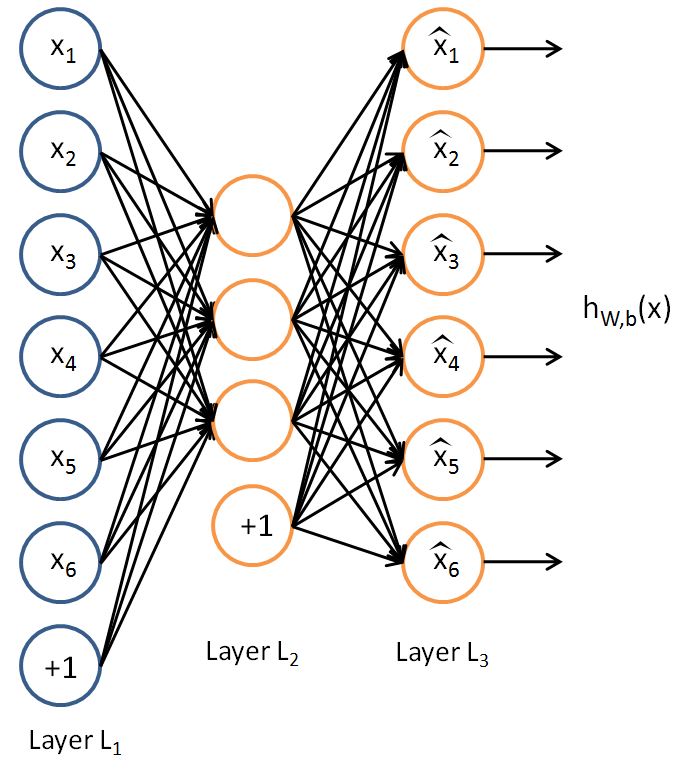
\includegraphics[width=0.5\textwidth]{figures/Autoencoder636.png}
  %\caption{}\label{fig:step1}
\end{figure}

\cnt{The autoencoder tries to learn a function $h_{W,b}(x) \approx x$. In other words, it is trying to learn an approximation to the identity function, so as to output $\hat{x}$ that is similar to $x$. The identity function seems a particularly trivial function to be trying to learn; but by placing constraints on the network, such as by limiting the number of hidden units, we can discover interesting structure about the data. As a concrete example, suppose the inputs $x$ are the pixel intensity values from a $10 \times 10$ image (100 pixels) so $n=100$, and there are $s_2=50$ hidden units in layer $L_2$. Note that we also have $y \in \Re^{100}$. Since there are only 50 hidden units, the network is forced to learn a compressed representation of the input. I.e., given only the vector of hidden unit activations $a^{(2)} \in \Re^{50}$, it must try to reconstruct the 100-pixel input $x$. If the input were completely random---say, each $x_i$ comes from an IID Gaussian independent of the other features---then this compression task would be very difficult. But if there is structure in the data, for example, if some of the input features are correlated, then this algorithm will be able to discover some of those correlations. In fact, this simple autoencoder often ends up learning a low-dimensional representation very similar to PCAs.}
    {自编码神经网络尝试学习一个 $h_{W,b}(x) \approx x$ 的函数。换句话说,它尝试逼近一个恒等函数,从而使得输出 $\hat{x}$ 接近于输入 $x$。恒等函数虽然看上去不太有学习的意义,但是当我们为自编码神经网络加入某些限制,比如限定隐藏神经元的数量,我们就可以从输入数据中发现一些有趣的结构。举例来说,假设某个自编码神经网络的输入 $x$ 是一张 $10 \times 10$ 图像(共100个像素)的像素灰度值,于是 $n=100$,其隐藏层 $L_2$ 中有 $50$ 个隐藏神经元。注意,输出也是100维的 $y \in \Re^{100}$。由于只有50个隐藏神经元,我们迫使自编码神经网络去学习输入数据的压缩表示,也就是说,它必须从50维的隐藏神经元激活度向量 $a^{(2)} \in \Re^{50}$ 中重构出100维的像素灰度值输入 $x$。如果网络的输入数据是完全随机的,比如每一个输入 $x_i$ 都是一个跟其它特征完全无关的独立同分布高斯随机变量,那么这一压缩表示将会非常难学习。但是如果输入数据中隐含着一些特定的结构,比如某些输入特征是彼此相关的,那么这一算法就可以发现输入数据中的这些相关性。事实上,这一简单的自编码神经网络通常可以学习出一个跟主元分析(PCA)结果非常相似的输入数据的低维表示。}
    {}


\cnt{Our argument above relied on the number of hidden units $s_2$ being small. But even when the number of hidden units is large (perhaps even greater than the number of input pixels), we can still discover interesting structure, by imposing other constraints on the network. In particular, if we impose a sparsity constraint on the hidden units, then the autoencoder will still discover interesting structure in the data, even if the number of hidden units is large.}
    {我们刚才的论述是基于隐藏神经元数量较小的假设。但是即使隐藏神经元的数量较大(可能比输入像素的个数还要多),我们仍然通过给自编码神经网络施加一些其他的限制条件来发现输入数据中的结构。具体来说,如果我们给隐藏神经元加入稀疏性限制,那么自编码神经网络即使在隐藏神经元数量较多的情况下仍然可以发现输入数据中一些有趣的结构。}
    {}

\cnt{Informally, we will think of a neuron as being ``active" (or as ``firing") if its output value is close to 1, or as being ``inactive" if its output value is close to 0. We would like to constrain the neurons to be inactive most of the time. This discussion assumes a sigmoid activation function. If you are using a tanh activation function, then we think of a neuron as being inactive when it outputs values close to -1.}
    {稀疏性可以被简单地解释如下。如果当神经元的输出接近于1的时候我们认为它被激活,而输出接近于0的时候认为它被抑制,那么使得神经元大部分的时间都是被抑制的限制则被称作稀疏性限制。这里我们假设的神经元的激活函数是sigmoid函数。如果你使用tanh作为激活函数的话,当神经元输出为-1的时候,我们认为神经元是被抑制的。}
    {}

\cnt{Recall that $a^{(2)}_j$ denotes the activation of hidden unit $j$ in the autoencoder. However, this notation doesn't make explicit what was the input $x$ that led to that activation. Thus, we will write $a^{(2)}_j(x)$ to denote the activation of this hidden unit when the network is given a specific input $x$. Further, let}
    {注意到 $a^{(2)}_j$ 表示隐藏神经元 $j$ 的激活度,但是这一表示方法中并未明确指出哪一个输入 $x$ 带来了这一激活度。所以我们将使用 $a^{(2)}_j(x)$ 来表示在给定输入为 $x$ 情况下,自编码神经网络隐藏神经元 $j$ 的激活度。 进一步,让}
    {}
\begin{align} \hat\rho_j = \frac{1}{m} \sum_{i=1}^m \left[ a^{(2)}_j(x^{(i)}) \right] \end{align}
\cnt{be the average activation of hidden unit $j$ (averaged over the training set). We would like to (approximately) enforce the constraint}
    {表示隐藏神经元 $j$ 的平均活跃度(在训练集上取平均)。我们可以近似的加入一条限制}
    {}
\begin{align} \hat\rho_j = \rho, \end{align}
\cnt{where $\rho$ is a sparsity parameter, typically a small value close to zero (say $\rho = 0.05$). In other words, we would like the average activation of each hidden neuron $j$ to be close to 0.05 (say). To satisfy this constraint, the hidden unit's activations must mostly be near 0.}
    {其中, $\rho$ 是稀疏性参数,通常是一个接近于0的较小的值(比如 $\rho = 0.05$)。换句话说,我们想要让隐藏神经元 $j$ 的平均活跃度接近0.05。为了满足这一条件,隐藏神经元的活跃度必须接近于0。}
    {}

\cnt{To achieve this, we will add an extra penalty term to our optimization objective that penalizes $\hat\rho_j$ deviating significantly from $\rho$. Many choices of the penalty term will give reasonable results. We will choose the following:}
    {为了实现这一限制,我们将会在我们的优化目标函数中加入一个额外的惩罚因子,而这一惩罚因子将惩罚那些 $\hat\rho_j$ 和 $\rho$ 有显著不同的情况从而使得隐藏神经元的平均活跃度保持在较小范围内。惩罚因子的具体形式有很多种合理的选择,我们将会选择以下这一种: }
    {}
\begin{align} \sum_{j=1}^{s_2} \rho \log \frac{\rho}{\hat\rho_j} + (1-\rho) \log \frac{1-\rho}{1-\hat\rho_j}. \end{align}

\cnt{Here, $s_2$ is the number of neurons in the hidden layer, and the index $j$ is summing over the hidden units in our network. If you are familiar with the concept of KL divergence, this penalty term is based on it, and can also be written}
    {这里, $s_2$ 是隐藏层中隐藏神经元的数量,而索引 $j$ 依次代表隐藏层中的每一个神经元。如果你对相对熵(KL divergence)比较熟悉,这一惩罚因子实际上是基于它的。于是惩罚因子也可以被表示为}
    {}
\begin{align} \sum_{j=1}^{s_2} {\rm KL}(\rho || \hat\rho_j), \end{align} 
\cnt{where ${\rm KL}(\rho || \hat\rho_j) = \rho \log \frac{\rho}{\hat\rho_j} + (1-\rho) \log \frac{1-\rho}{1-\hat\rho_j}$ is the Kullback-Leibler (KL) divergence between a Bernoulli random variable with mean $\rho$ and a Bernoulli random variable with mean $\hat\rho_j$. KL-divergence is a standard function for measuring how different two different distributions are. (If you've not seen KL-divergence before, don't worry about it; everything you need to know about it is contained in these notes.)}
    {其中 ${\rm KL}(\rho || \hat\rho_j) = \rho \log \frac{\rho}{\hat\rho_j} + (1-\rho) \log \frac{1-\rho}{1-\hat\rho_j}$ 是一个以 $\rho$ 为均值和一个以 $\hat\rho_j$ 为均值的两个伯努利随机变量之间的相对熵。相对熵是一种标准的用来测量两个分布之间差异的方法。(如果你没有见过相对熵,不用担心,所有你需要知道的内容都会被包含在这份笔记之中。)}
    {}

\cnt{This penalty function has the property that ${\rm KL}(\rho || \hat\rho_j) = 0$ if $\hat\rho_j = \rho$, and otherwise it increases monotonically as $\hat\rho_j$ diverges from $\rho$. For example, in the figure below, we have set $\rho = 0.2$, and plotted ${\rm KL}(\rho || \hat\rho_j)$ for a range of values of $\hat\rho_j$:}
    {这一惩罚因子有如下性质,当 $\hat\rho_j = \rho$ 时 ${\rm KL}(\rho || \hat\rho_j) = 0$,并且随着 $\hat\rho_j$ 与 $\rho$ 之间的差异增大而单调递增。举例来说,在下图中,我们设定 $\rho = 0.2$ 并且画出了相对熵值 ${\rm KL}(\rho || \hat\rho_j)$ 随着 $\hat\rho_j$ 变化的变化。}
    {}

\begin{figure}[ht] \centering
  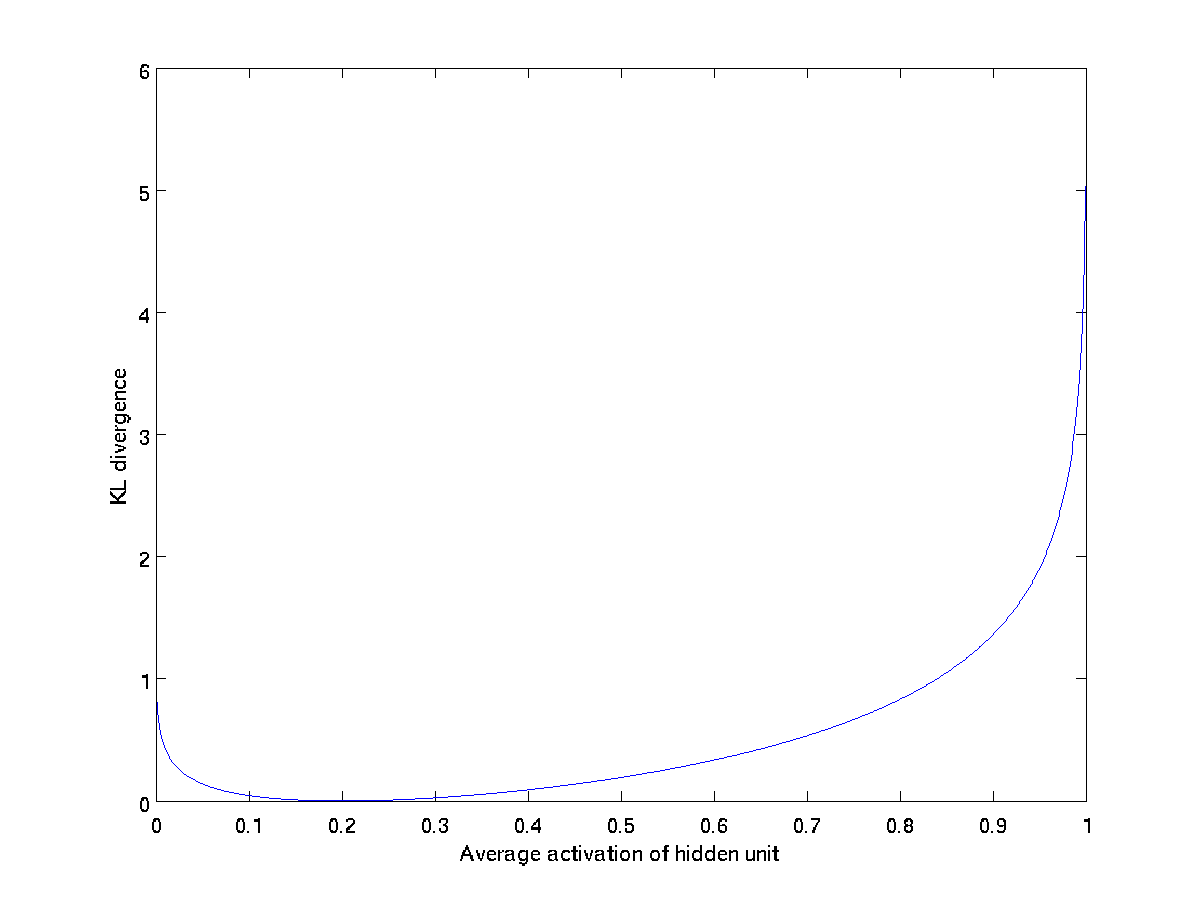
\includegraphics[width=0.8\textwidth]{figures/KLPenaltyExample.png}
  %\caption{}\label{fig:step1}
\end{figure}


\cnt{We see that the KL-divergence reaches its minimum of 0 at $\hat\rho_j = \rho$, and blows up (it actually approaches $\infty$) as $\hat\rho_j$ approaches $0$ or $1$. Thus, minimizing this penalty term has the effect of causing $\hat\rho_j$ to be close to $\rho$.}
    {我们可以看出,相对熵在 $\hat\rho_j = \rho$ 时达到它的最小值0,而当 $\hat\rho_j$ 靠近0或者1的时候,相对熵则变得非常大(其实是趋向于 $\infty$)。所以,最小化这一惩罚因子具有使得 $\hat\rho_j$ 靠近 $\rho$ 的效果。}
    {}


\cnt{Our overall cost function is now}
    {现在,我们的总体代价函数可以表示为}
    {}
\begin{align} J_{\rm sparse}(W,b) = J(W,b) + \beta \sum_{j=1}^{s_2} {\rm KL}(\rho || \hat\rho_j), \end{align}
\cnt{where $J(W,b)$ is as defined previously, and $\beta$ controls the weight of the sparsity penalty term. The term $\hat\rho_j$ (implicitly) depends on $W,b$ also, because it is the average activation of hidden unit $j$, and the activation of a hidden unit depends on the parameters $W,b$.}
    {其中 $J(W,b)$ 如之前所定义,而 $\beta$ 控制稀疏性惩罚因子的权重。 $\hat\rho_j$ 项则也(间接地)取决于 $W,b$,因为它是隐藏神经元 $j$ 的平均激活度,而隐藏层神经元的激活度取决于 $W,b$。}
    {}

\cnt{To incorporate the KL-divergence term into your derivative calculation, there is a simple-to-implement trick involving only a small change to your code. Specifically, where previously for the second layer ($l=2$), during backpropagation you would have computed}
    {为了对相对熵进行导数计算,我们可以使用一个易于实现的技巧,这只需要在你的程序中稍作改动即可。具体来说,前面在后向传播算法中计算第二层( $l=2$ )更新的时候我们已经计算了}
    {}
\begin{align} \delta^{(2)}_i = \left( \sum_{j=1}^{s_{2}} W^{(2)}_{ji} \delta^{(3)}_j \right) f'(z^{(2)}_i), \end{align} 
\cnt{now instead compute}
    {现在我们将其换成}
    {}
\begin{align} \delta^{(2)}_i = \left( \left( \sum_{j=1}^{s_{2}} W^{(2)}_{ji} \delta^{(3)}_j \right) + \beta \left( - \frac{\rho}{\hat\rho_i} + \frac{1-\rho}{1-\hat\rho_i} \right) \right) f'(z^{(2)}_i) . \end{align} 
\cnt{}{就可以了。}{}


\cnt{One subtlety is that you'll need to know $\hat\rho_i$ to compute this term. Thus, you'll need to compute a forward pass on all the training examples first to compute the average activations on the training set, before computing backpropagation on any example. If your training set is small enough to fit comfortably in computer memory (this will be the case for the programming assignment), you can compute forward passes on all your examples and keep the resulting activations in memory and compute the $\hat\rho_is$. Then you can use your precomputed activations to perform backpropagation on all your examples. If your data is too large to fit in memory, you may have to scan through your examples computing a forward pass on each to accumulate (sum up) the activations and compute $\hat\rho_i$ (discarding the result of each forward pass after you have taken its activations $a^{(2)}_i$ into account for computing $\hat\rho_i$). Then after having computed $\hat\rho_i$, you'd have to redo the forward pass for each example so that you can do backpropagation on that example. In this latter case, you would end up computing a forward pass twice on each example in your training set, making it computationally less efficient.}
    {有一个需要注意的地方就是我们需要知道 $\hat\rho_i$ 来计算这一项更新。所以在计算任何神经元的后向传播之前,你需要对所有的训练样本计算一遍前向传播,从而获取平均激活度。如果你的训练样本可以小到被整个存到内存之中(对于编程作业来说,通常如此),你可以方便地在你所有的样本上计算前向传播并将得到的激活度存入内存并且计算平均激活度 。然后你就可以使用事先计算好的激活度来对所有的训练样本进行后向传播的计算。如果你的数据量太大,无法全部存入内存,你就可以扫过你的训练样本并计算一次前向传播,然后将获得的结果累积起来并计算平均激活度 $\hat\rho_i$ (当某一个前向传播的结果中的激活度 $a^{(2)}_i$ 被用于计算平均激活度 $\hat\rho_i$ 之后就可以将此结果删除)。然后当你完成平均激活度 $\hat\rho_i$ 的计算之后,你需要重新对每一个训练样本做一次前向传播从而可以对其进行后向传播的计算。对于后一种情况,你对每一个训练样本需要计算两次前向传播,所以在计算上的效率会稍低一些。}
    {}

\cnt{The full derivation showing that the algorithm above results in gradient descent is beyond the scope of these notes. But if you implement the autoencoder using backpropagation modified this way, you will be performing gradient descent exactly on the objective $J_{\rm sparse}(W,b)$. Using the derivative checking method, you will be able to verify this for yourself as well.}
    {证明上面算法能达到梯度下降效果的完整推导过程不再本教程的范围之内。不过如果你想要使用经过以上修改的后向传播来实现自编码神经网络,那么你就会对目标函数 $J_{\rm sparse}(W,b)$ 做梯度下降。使用梯度验证方法,你可以自己来验证梯度下降算法是否正确。}
    {}

\subsection{\cnt{Visualizing a Trained Autoencoder}{可视化自编码器训练结果}{}}

\cnt{Having trained a (sparse) autoencoder, we would now like to visualize the function learned by the algorithm, to try to understand what it has learned. Consider the case of training an autoencoder on $10 \times 10$ images, so that $n = 100$. Each hidden unit $i$ computes a function of the input:}
    {训练完(稀疏)自编码器,我们还想把这自编码器学到的函数可视化出来,好弄明白它到底学到了什么。我们以在$10 \times 10$图像(即n=100)上训练自编码器为例。在该自编码器中,每个隐藏单元i对如下关于输入的函数进行计算:}
    {}
\begin{align} a^{(2)}_i = f\left(\sum_{j=1}^{100} W^{(1)}_{ij} x_j + b^{(1)}_i \right). \end{align} 

\cnt{We will visualize the function computed by hidden unit $i$ --- which depends on the parameters $W^{(1)}_{ij}$ (ignoring the bias term for now)---using a 2D image. In particular, we think of $a^{(2)}_i$ as some non-linear feature of the input $x$. We ask: What input image $x$ would cause $a^{(2)}_i$ to be maximally activated? (Less formally, what is the feature that hidden unit $i$ is looking for?) For this question to have a non-trivial answer, we must impose some constraints on $x$. If we suppose that the input is norm constrained by $||x||^2 = \sum_{i=1}^{100} x_i^2 \leq 1$, then one can show (try doing this yourself) that the input which maximally activates hidden unit $i$ is given by setting pixel $x_j$ (for all 100 pixels, $j=1,\ldots, 100$) to}
    {我们将要可视化的函数,就是上面这个以2D图像为输入、并由隐藏单元i计算出来的函数。它是依赖于参数 $W^{(1)}_{ij}$ 的(暂时忽略偏置项 $b_i$)。需要注意的是,$a^{(2)}_i$ 可看作输入 $x$ 的非线性特征。不过还有个问题:什么样的输入图像 $x$ 可让 $a^{(2)}_i$ 得到最大程度的激励?(通俗一点说,隐藏单元 $i$ 要找个什么样的特征?)。这里我们必须给 $x$ 加约束,否则会得到平凡解。若假设输入有范数约束 $||x||^2 = \sum_{i=1}^{100} x_i^2 \leq 1$,则可证(请读者自行推导)令隐藏单元 $i$ 得到最大激励的输入应由下面公式计算的像素 $x_j$ 给出(共需计算100个像素,$j=1,\ldots, 100$):}
    {}
\begin{align} x_j = \frac{W^{(1)}_{ij}}{\sqrt{\sum_{j=1}^{100} (W^{(1)}_{ij})^2}}. \end{align} 

\cnt{By displaying the image formed by these pixel intensity values, we can begin to understand what feature hidden unit $i$ is looking for.}
    {当我们用上式算出各像素的值、把它们组成一幅图像、并将图像呈现在我们面前之时,隐藏单元 $i$ 所追寻特征的真正含义也渐渐明朗起来。}
    {}

\cnt{If we have an autoencoder with 100 hidden units (say), then we our visualization will have 100 such images---one per hidden unit. By examining these 100 images, we can try to understand what the ensemble of hidden units is learning.}
    {假如我们训练的自编码器有100个隐藏单元,可视化结果就会包含100幅这样的图像——每个隐藏单元都对应一幅图像。审视这100幅图像,我们可以试着体会这些隐藏单元学出来的整体效果是什么样的。}
    {}


\cnt{When we do this for a sparse autoencoder (trained with 100 hidden units on 10x10 pixel inputs)}
    {当我们对稀疏自编码器进行上述可视化处理之后(100个隐藏单元,在10X10像素的输入上训练),}
    {}
\footnote{
\cnt{The learned features were obtained by training on \emph{whitened} natural images. Whitening is a preprocessing step which removes redundancy in the input, by causing adjacent pixels to become less correlated.}
    {}
    {}
}
\cnt{we get the following result:}
    {结果如下所示:}
    {}

\begin{figure}[ht] \centering
  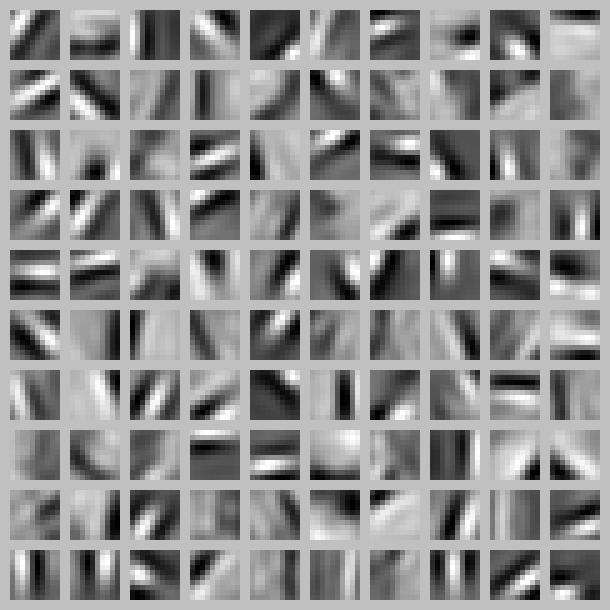
\includegraphics[width=0.5\textwidth]{figures/ExampleSparseAutoencoderWeights.png}
  %\caption{}\label{fig:step1}
\end{figure}

\cnt{Each square in the figure above shows the (norm bounded) input image $x$ that maximally actives one of 100 hidden units. We see that the different hidden units have learned to detect edges at different positions and orientations in the image.}
    {上图的每个小方块都给出了一个(带有有界范数 的)输入图像 $x$,它可使这100个隐藏单元中的某一个获得最大激励。我们可以看到,不同的隐藏单元学会了在图像的不同位置和方向进行边缘检测。}
    {}


\cnt{These features are, not surprisingly, useful for such tasks as object recognition and other vision tasks. When applied to other input domains (such as audio), this algorithm also learns useful representations/features for those domains too.}
    {显而易见,这些特征对物体识别等计算机视觉任务是十分有用的。若将其用于其他输入域(如音频),该算法也可学到对这些输入域有用的表示或特征。}
    {}

\subsection{\cnt{Sparse Autoencoder Notation Summary}{稀疏自编码器符号一览表}{}}

\cnt{Here is a summary of the symbols used in our derivation of the sparse autoencoder:}
    {下面是我们在推导sparse autoencoder时使用的符号一览表:}
    {}

\begin{longtable}[h]{>{\centering\arraybackslash}m{0.1\textwidth}m{0.7\textwidth}}
\caption{\cnt{Sparse Autoencoder Notation Summary}{稀疏自编码器符号一览表}{}} \label{tab:sparseautoencodersummary}\\
\toprule
\textbf{\cnt{Symbol}{符号}{}}&\textbf{\cnt{Meaning}{含义}{}} \\
\midrule
\endfirsthead  % endfirsthead 以上內容只出現在第一頁
\midrule
\textbf{\cnt{Symbol}{符号}{}}&\textbf{\cnt{Meaning}{含义}{}} \\
\midrule
\endhead % endfirsthead 及 endhead 間的內容會排版至每頁上方
%\midrule
\multicolumn{2}{r}{\cnt{To be continued}{续下页}{} \dots} \\
\midrule

\endfoot % endfoot 以上的內會出現在每頁底部
\endlastfoot

$x$	& \cnt{Input features for a training example, $x \in \Re^{n}$.}{训练样本的输入特征,$x \in \Re^{n}$.}{} \\
  \midrule

$y$	& \cnt{Output/target values. Here, $y$ can be vector valued. In the case of an autoencoder, $y=x$.}{输出值/目标值. 这里 $y$ 可以是向量. 在autoencoder中,$y=x$.}{} \\
  \midrule

$(x^{(i)}, y^{(i)})$	& \cnt{The $i$-th training example}{第 $i$ 个训练样本}{} \\
  \midrule

$h_{W,b}(x)$	& \cnt{Output of our hypothesis on input $x$, using parameters $W,b$. This should be a vector of the same dimension as the target value $y$.}{输入为 $x$ 时的假设输出,其中包含参数 $W,b$. 该输出应当与目标值 $y$ 具有相同的维数.}{} \\
  \midrule

$W^{(l)}_{ij}$	& \cnt{The parameter associated with the connection between unit $j$ in layer $l$, and unit $i$ in layer $l+1$.}{连接第 $l$ 层 $j$ 单元和第 $l+1$ 层 $i$ 单元的参数.}{} \\
  \midrule

$b^{(l)}_{i}$	& \cnt{The bias term associated with unit $i$ in layer $l+1$. Can also be thought of as the parameter associated with the connection between the bias unit in layer $l$ and unit $i$ in layer $l+1$.}{第 $l+1$ 层 $i$ 单元的偏置项. 也可以看作是连接第 $l$ 层偏置单元和第 $l+1$ 层 $i$ 单元的参数.}{} \\
  \midrule

$\theta$	& \cnt{Our parameter vector. It is useful to think of this as the result of taking the parameters $W,b$ and ``unrolling them into a long column vector.}{参数向量. 可以认为该向量是通过将参数 $W,b$ 组合展开为一个长的列向量而得到.}{} \\
  \midrule

$a^{(l)}_i$	& \cnt{Activation (output) of unit $i$ in layer $l$ of the network. In addition, since layer $L_1$ is the input layer, we also have $a^{(1)}_i = x_i$.}{网络中第 $l$ 层 $i$ 单元的激活(输出)值. 另外,由于 $L_1$ 层是输入层,所以 $a^{(1)}_i = x_i$.}{} \\
  \midrule

$f(\cdot)$	& \cnt{The activation function. Throughout these notes, we used $f(z) = \tanh(z)$.}{激活函数. 本文中我们使用 $f(z) = \tanh(z)$.}{} \\
  \midrule

$z^{(l)}_i$	& \cnt{Total weighted sum of inputs to unit $i$ in layer $l$. Thus, $a^{(l)}_i = f(z^{(l)}_i)$.}{第 $l$ 层 $i$ 单元所有输入的加权和. 因此有 $a^{(l)}_i = f(z^{(l)}_i)$.}{} \\
  \midrule

$\alpha$	& \cnt{Learning rate parameter}{学习率}{} \\
  \midrule

$s_l$	& \cnt{Number of units in layer $l$ (not counting the bias unit).}{第 $l$ 层的单元数目(不包含偏置单元).}{} \\
  \midrule

$n_l$	& \cnt{Number layers in the network. Layer $L_1$ is usually the input layer, and layer $L_{n_l}$ the output layer.}{网络中的层数. 通常 $L_1$ 层是输入层,$L_{n_l}$ 层是输出层.}{} \\
  \midrule

$\lambda$	& \cnt{Weight decay parameter.}{权重衰减系数.}{} \\
  \midrule

$\hat{x}$	& \cnt{For an autoencoder, its output; i.e., its reconstruction of the input $x$. Same meaning as $h_{W,b}(x)$.}{对于一个autoencoder,该符号表示其输出值;亦即输入值 $x$ 的重构值. 与 $h_{W,b}(x)$ 含义相同.}{} \\
  \midrule

$\rho$	& \cnt{Sparsity parameter, which specifies our desired level of sparsity}{稀疏值,可以用它指定我们所需的稀疏程度}{} \\
  \midrule

$\hat\rho_i$	& \cnt{The average activation of hidden unit $i$ (in the sparse autoencoder).}{(sparse autoencoder中)隐藏单元 $i$ 的平均激活值.}{} \\
  \midrule

$\beta$	& \cnt{Weight of the sparsity penalty term (in the sparse autoencoder objective).}{(sparse autoencoder目标函数中)稀疏值惩罚项的权重.}{} \\

\bottomrule
\end{longtable}

\subsection{\cnt{Exercise: Sparse Autoencoder}{练习:稀疏自编码器}{}} \label{chp:execsparseautoenc}


\cnt{You may want to download the related document from \url{http://nlp.stanford.edu/~socherr/sparseAutoencoder_2011new.pdf} and \url{http://www.stanford.edu/class/cs294a/cs294a_2011-assignment.pdf}.}
    {可以从 \url{http://nlp.stanford.edu/~socherr/sparseAutoencoder_2011new.pdf} 和 \url{http://www.stanford.edu/class/cs294a/cs294a_2011-assignment.pdf} 下载文档。}
    {}

\textbf{\cnt{Sparse autoencoder implementation}{稀疏自编码器的实现}{}}

\cnt{In this problem set, you will implement the sparse autoencoder algorithm, and show how it discovers that edges are a good representation for natural images. (Images provided by Bruno Olshausen.) The sparse autoencoder algorithm is described in the lecture notes found on the course website. }
    {}
    {}


\cnt{In the file
%\href{http://ufldl.stanford.edu/wiki/resources/sparseae_exercise.zip}{sparseae_exercise.zip}
\url{http://ufldl.stanford.edu/wiki/resources/sparseae_exercise.zip}
, we have provided some starter code in Matlab. You should write your code at the places indicated in the files (\texttt{``YOUR CODE HERE"}). You have to complete the following files: \texttt{sampleIMAGES.m, sparseAutoencoderCost.m, computeNumericalGradient.m}. The starter code in \texttt{train.m} shows how these functions are used.}
    {}
    {}


\cnt{Specifically, in this exercise you will implement a sparse autoencoder, trained with $8 \times 8$ image patches using the L-BFGS optimization algorithm.}
    {}
    {}


\cnt{\emph{A note on the software}: The provided .zip file includes a subdirectory \texttt{minFunc} with 3rd party software implementing L-BFGS, that is licensed under a Creative Commons, Attribute, Non-Commercial license. If you need to use this software for commercial purposes, you can download and use a different function (fminlbfgs) that can serve the same purpose, but runs $~ 3 \times $ slower for this exercise (and thus is less recommended). You can read more about this in the
%\href{http://deeplearning.stanford.edu/wiki/index.php/Fminlbfgs_Details}{Fminlbfgs_Details}
\url{http://deeplearning.stanford.edu/wiki/index.php/Fminlbfgs_Details}
page.}
    {}
    {}


\subsubsection{\cnt{Step 1: Generate training set}{第一步:生成训练集}{}}

\cnt{The first step is to generate a training set. To get a single training example $x$, randomly pick one of the 10 images, then randomly sample an $8 \times 8$ image patch from the selected image, and convert the image patch (either in row-major order or column-major order; it doesn't matter) into a 64-dimensional vector to get a training example $x \in \Re^{64}$.}
    {}
    {}

\cnt{Complete the code in \texttt{sampleIMAGES.m}. Your code should sample 10000 image patches and concatenate them into a $64 \times 10000$ matrix. }
    {}
    {}

\cnt{To make sure your implementation is working, run the code in ``Step 1" of train.m. This should result in a plot of a random sample of 200 patches from the dataset.}
    {}
    {}

\cnt{\emph{Implementational tip}: When we run our implemented \texttt{sampleImages()}, it takes under 5 seconds. If your implementation takes over 30 seconds, it may be because you are accidentally making a copy of an entire $512 \times 512$ image each time you're picking a random image. By copying a $512 \times 512$ image 10000 times, this can make your implementation much less efficient. While this doesn't slow down your code significantly for this exercise (because we have only 10000 examples), when we scale to much larger problems later this quarter with $10^6$ or more examples, this will significantly slow down your code. Please implement \texttt{sampleIMAGES} so that you aren't making a copy of an entire $512 \times 512$ image each time you need to cut out an $8 \times 8$ image patch. }
    {}
    {}

\subsubsection{\cnt{Step 2: Sparse autoencoder objective}{第二步:稀疏自编码器}{}}

\cnt{Implement code to compute the sparse autoencoder cost function $J_{sparse}(W,b)$ (Section 3 of the lecture notes) and the corresponding derivatives of $J_{sparse}$ with respect to the different parameters. Use the sigmoid function for the activation function, $f(z) = \frac{1}{{1+e^{-z}}}$. In particular, complete the code in \texttt{sparseAutoencoderCost.m}. }
    {}
    {}

\cnt{The sparse autoencoder is parameterized by matrices $W^{(1)} \in \Re^{s_1\times s_2}, W^{(2)} \in \Re^{s_2\times s_3}$ vectors $b^{(1)} \in \Re^{s_2}, b^{(2)} \in \Re^{s_3}$. However, for subsequent notational convenience, we will ``unroll" all of these parameters into a very long parameter vector $\theta$ with $s_1s_2 + s_2s_3 + s_2 + s_3$ elements. The code for converting between the $(W^{(1)},W^{(2)},b^{(1)},b^{(2)})$ and the $\theta$ parameterization is already provided in the starter code.}
    {}
    {}



\cnt{\emph{Implementational tip}: The objective $J_{sparse}(W,b)$ contains 3 terms, corresponding to the squared error term, the weight decay term, and the sparsity penalty. You're welcome to implement this however you want, but for ease of debugging, you might implement the cost function and derivative computation (backpropagation) only for the squared error term first (this corresponds to setting $\lambda = \beta = 0$), and implement the gradient checking method in the next section to first verify that this code is correct. Then only after you have verified that the objective and derivative calculations corresponding to the squared error term are working, add in code to compute the weight decay and sparsity penalty terms and their corresponding derivatives. }
    {}
    {}


\subsubsection{\cnt{Step 3: Gradient checking}{第三步:梯度检测}{}}

\cnt{Following Section 2.3 of the lecture notes, implement code for gradient checking. Specifically, complete the code in \texttt{computeNumericalGradient.m}. Please use ${\rm EPSILON} = 10^{-4}$ as described in the lecture notes.}
    {}
    {}

\cnt{We've also provided code in checkNumericalGradient.m for you to test your code. This code defines a simple quadratic function $h: \Re^2 \mapsto \Re$ given by $h(x) = x_1^2 + 3x_1 x_2$, and evaluates it at the point $x = (4,10)^T$. It allows you to verify that your numerically evaluated gradient is very close to the true (analytically computed) gradient.}
    {}
    {}

\cnt{After using checkNumericalGradient.m to make sure your implementation is correct, next use computeNumericalGradient.m to make sure that your sparseAutoencoderCost.m is computing derivatives correctly. For details, see Steps 3 in train.m. We strongly encourage you not to proceed to the next step until you've verified that your derivative computations are correct. }
    {}
    {}

\cnt{\emph{Implementational tip}: If you are debugging your code, performing gradient checking on smaller models and smaller training sets (e.g., using only 10 training examples and 1-2 hidden units) may speed things up. }
    {}
    {}

\subsubsection{\cnt{Step 4: Train the sparse autoencoder}{第四步:训练稀疏自编码器}{}}

\cnt{Now that you have code that computes Jsparse and its derivatives, we're ready to minimize Jsparse with respect to its parameters, and thereby train our sparse autoencoder. }
    {}
    {}

\cnt{We will use the L-BFGS algorithm. This is provided to you in a function called minFunc (code provided by Mark Schmidt) included in the starter code. (For the purpose of this assignment, you only need to call minFunc with the default parameters. You do not need to know how L-BFGS works.) We have already provided code in train.m (Step 4) to call minFunc. The minFunc code assumes that the parameters to be optimized are a long parameter vector; so we will use the ``$\theta$" parameterization rather than the ``$(W^{(1)},W^{(2)},b^{(1)},b^{(2)})$" parameterization when passing our parameters to it. }
    {}
    {}

\cnt{Train a sparse autoencoder with 64 input units, 25 hidden units, and 64 output units. In our starter code, we have provided a function for initializing the parameters. We initialize the biases $b^{(l)}_i$ to zero, and the weights $W^{(l)}_{ij}$ to random numbers drawn uniformly from the interval $\left[-\sqrt{\dfrac{6}{n_{\rm in}+n_{\rm out}+1}},\sqrt{\dfrac{6}{n_{\rm in}+n_{\rm out}+1}}\,\right]$, where $n_{in}$ is the fan-in (the number of inputs feeding into a node) and $n_{out}$ is the fan-in (the number of units that a node feeds into). }
    {}
    {}

\cnt{The values we provided for the various parameters ($\lambda ,\beta ,\rho$, etc.) should work, but feel free to play with different settings of the parameters as well.}
    {}
    {}

\cnt{\emph{Implementational tip}: Once you have your backpropagation implementation correctly computing the derivatives (as verified using gradient checking in Step 3), when you are now using it with L-BFGS to optimize $J_{sparse}(W,b)$, make sure you're not doing gradient-checking on every step. Backpropagation can be used to compute the derivatives of Jsparse(W,b) fairly efficiently, and if you were additionally computing the gradient numerically on every step, this would slow down your program significantly.}
    {}
    {}

\subsubsection{\cnt{Step 5: Visualization}{第五步:可视化}{}}

\cnt{After training the autoencoder, use \texttt{display\_network.m} to visualize the learned weights. (See \texttt{train.m}, Step 5.) Run ``\texttt{print -djpeg weights.jpg}" to save the visualization to a file ``\texttt{weights.jpg}" (which you will submit together with your code).}
    {}
    {}

\textbf{
\cnt{Results}
    {结果}
    {}
}


\cnt{To successfully complete this assignment, you should demonstrate your sparse autoencoder algorithm learning a set of edge detectors. For example, this was the visualization we obtained:}
    {}
    {}

\begin{figure}[ht] \centering
  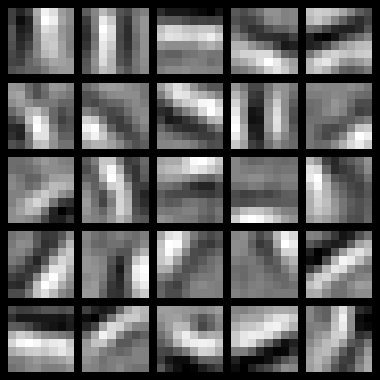
\includegraphics[width=0.5\textwidth]{figures/Gabor.jpg}
  %\caption{}\label{fig:step1}
\end{figure}

\cnt{Our implementation took around 5 minutes to run on a fast computer. In case you end up needing to try out multiple implementations or different parameter values, be sure to budget enough time for debugging and to run the experiments you'll need.}
    {}
    {}

\cnt{Also, by way of comparison, here are some visualizations from implementations that we do not consider successful (either a buggy implementation, or where the parameters were poorly tuned):}
    {}
    {}

\begin{figure}[ht] \centering
  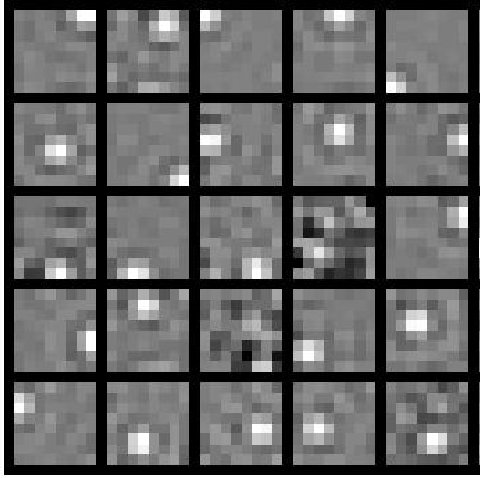
\includegraphics[width=0.3\textwidth]{figures/Badfilter1.jpg}
  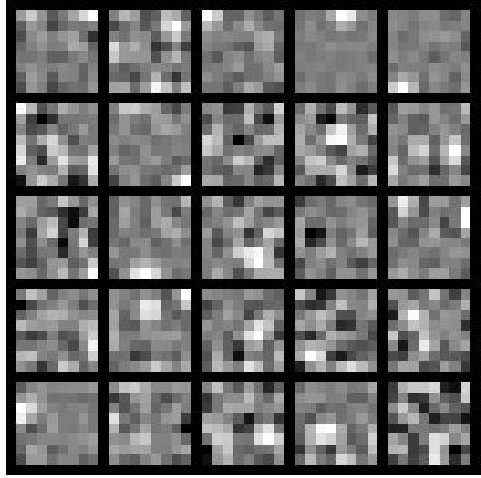
\includegraphics[width=0.3\textwidth]{figures/Badfilter2.jpg}
  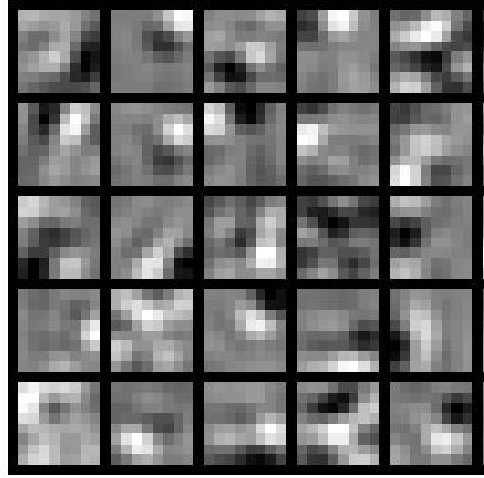
\includegraphics[width=0.3\textwidth]{figures/Badfilter3.jpg}
  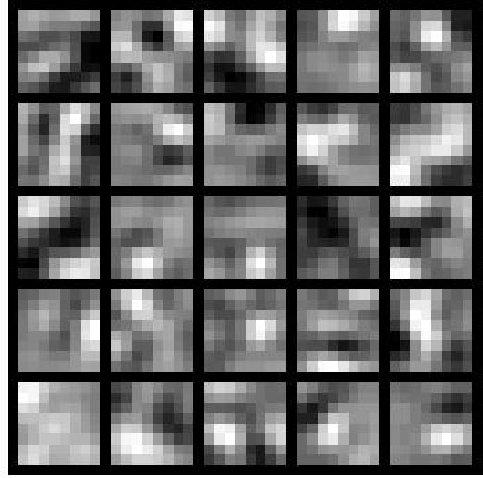
\includegraphics[width=0.3\textwidth]{figures/Badfilter4.jpg}
  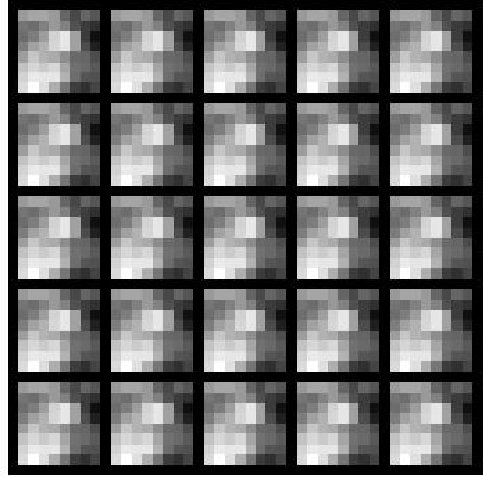
\includegraphics[width=0.3\textwidth]{figures/Badfilter5.jpg}
  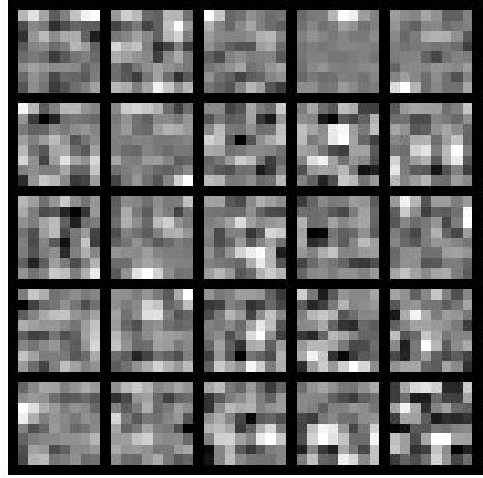
\includegraphics[width=0.3\textwidth]{figures/Badfilter6.jpg}
  %\caption{}\label{fig:step1}
\end{figure}


\clearpage
%# -*- coding: utf-8 -*-
%!TEX encoding = UTF-8 Unicode
%!TEX TS-program = xelatex
% vim:ts=4:sw=4
%
% 以上设定默认使用 XeLaTex 编译,并指定 Unicode 编码,供 TeXShop 自动识别

% Author: Yunhui Fu <yhfudev@gmail.com>
% License: Creative Commons (CC BY 4.0)

\section{\cnt{Vectorized implementation}{矢量化编程实现}{}}

\subsection{\cnt{Vectorization}{矢量化编程}{}} \label{chp:vectorzation}

\cnt{When working with learning algorithms, having a faster piece of code often means that you'll make progress faster on your project. For example, if your learning algorithm takes 20 minutes to run to completion, that means you can ``try" up to 3 new ideas per hour. But if your code takes 20 hours to run, that means you can ``try" only one idea a day, since that's how long you have to wait to get feedback from your program. In this latter case, if you can speed up your code so that it takes only 10 hours to run, that can literally double your personal productivity!}
    {当使用学习算法时,一段更快的代码通常意味着项目进展更快。例如,如果你的学习算法需要花费20分钟运行完成,这意味着你每个小时能“尝试”3个新主意。但是假如你的程序需要20个小时来运行,这意味着你一天只能“尝试”一个新主意,因为你需要花费这么长时间来等待程序的反馈。对于后者,假如你可以提升代码的效率让其只需要运行10个小时,那么你的效率差不多提升一倍。}
    {}

\cnt{\emph{Vectorization} refers to a powerful way to speed up your algorithms. Numerical computing and parallel computing researchers have put decades of work into making certain numerical operations (such as matrix-matrix multiplication, matrix-matrix addition, matrix-vector multiplication) fast. The idea of vectorization is that we would like to express our learning algorithms in terms of these highly optimized operations.}
    {\emph{矢量化编程}是提高算法速度的一种有效方法。为了提升特定数值运算操作(如矩阵相乘、矩阵相加、矩阵-向量乘法等)的速度,数值计算和并行计算的研究人员已经努力了几十年。矢量化编程的思想就是尽量使用这些被高度优化的数值运算操作来实现我们的学习算法。}
    {}

\cnt{For example, if $x \in \Re^{n+1}$ and $\theta \in \Re^{n+1}$ are vectors and you need to compute $z = \theta^Tx$, you can implement (in Matlab):}
    {例如,假设 $x \in \Re^{n+1}$ 和 $\theta \in \Re^{n+1}$ 为向量,需要计算 $z = \theta^Tx$,那么可以按以下方式实现(使用Matlab):}
    {}

\begin{lstlisting}[language=matlab]
z = 0;
for i=1:(n+1),
  z = z + theta(i) * x(i);
end;
\end{lstlisting}

\cnt{or you can more simply implement}
    {或者可以更加简单的写为:}
    {}
\begin{lstlisting}[language=matlab]
z = theta' * x;
\end{lstlisting}


\cnt{The second piece of code is not only simpler, but it will also run \emph{much} faster.}
    {第二段程序代码不仅简单,而且\emph{运行速度更快}。}
    {}


\cnt{More generally, a good rule-of-thumb for coding Matlab/Octave is:}
    {通常,一个编写Matlab/Octave程序的诀窍是:}
    {}

{\center \bf
\cnt{Whenever possible, avoid using explicit for-loops in your code.}
    {代码中尽可能避免显式的for循环。}
    {}
}

\cnt{In particular, the first code example used an explicit \texttt{for} loop. By implementing the same functionality without the \texttt{for} loop, we sped it up significantly. A large part of vectorizing our Matlab/Octave code will focus on getting rid of \texttt{for} loops, since this lets Matlab/Octave extract more parallelism from your code, while also incurring less computational overhead from the interpreter.}
    {上面的第一段代码使用了一个显式的\texttt{for}循环。通过不使用\texttt{for}循环实现相同功能,可以显著提升运行速度。对Matlab/Octave代码进行矢量化的工作很大一部分集中在避免使用\texttt{for}循环上,因为这可以使得Matlab/Octave更多地利用代码中的并行性,同时其解释器的计算开销更小。}
    {}

\cnt{In terms of a strategy for writing your code, initially you may find that vectorized code is harder to write, read, and/or debug, and that there may be a tradeoff in ease of programming/debugging vs. running time. Thus, for your first few programs, you might choose to first implement your algorithm without too many vectorization tricks, and verify that it is working correctly (perhaps by running on a small problem). Then only after it is working, you can vectorize your code one piece at a time, pausing after each piece to verify that your code is still computing the same result as before. At the end, you'll then hopefully have a correct, debugged, and vectorized/efficient piece of code.}
    {关于编写代码的策略,开始时你会觉得矢量化代码更难编写、阅读和调试,但你需要在编码和调试的便捷性与运行时间之间做个权衡。因此,刚开始编写程序的时候,你可能会选择不使用太多矢量化技巧来实现你的算法,并验证它是否正确(可能只在一个小问题上验证)。在确定它正确后,你可以每次只矢量化一小段代码,并在这段代码之后暂停,以验证矢量化后的代码计算结果和之前是否相同。最后,你会有望得到一份正确的、经过调试的、矢量化且有效率的代码。}
    {}

\cnt{After you become familiar with the most common vectorization methods and tricks, you'll find that it usually isn't much effort to vectorize your code. Doing so will make your code run much faster and, in some cases, simplify it too.}
    {一旦对矢量化常见的方法和技巧熟悉后,你将会发现对代码进行矢量化通常并不太费劲。矢量化可以使你的代码运行的更快,而且在某些情况下,还简化了你的代码。}
    {}

\subsection{\cnt{Logistic Regression Vectorization Example}{逻辑回归的向量化实现样例}{}} \label{chp:logisticvecexample}

\cnt{Consider training a logistic regression model using batch gradient ascent. Suppose our hypothesis is}
    {我们想用批量梯度上升法对logistic回归分析模型进行训练,其模型如下:}
    {}
\begin{align} h_\theta(x) = \frac{1}{1+\exp(-\theta^Tx)}, \end{align}
\cnt{where (following the notational convention from the OpenClassroom videos and from CS229) we let $x_0=1$, so that $x \in \Re^{n+1}$ and $\theta \in \Re^{n+1}$, and $\theta_0$ is our intercept term. We have a training set $\{\left(x^{(1)}, y^{(1)}\right), \ldots, \left(x^{(m)}, y^{(m)}\right)\}$ of $m$ examples, and the batch gradient ascent update rule is $\theta := \theta + \alpha \nabla_\theta \ell(\theta)$, where $\ell(\theta)$ is the log likelihood and $\nabla_\theta \ell(\theta)$ is its derivative.}
    {
让我们遵从公开课程视频与CS229教学讲义的符号规范,
设 $x_0=1$,于是 $x \in \Re^{n+1}$,$\theta \in \Re^{n+1}$, $\theta_0$ 为截距。
假设我们有 $m$ 个训练样本 $\{\left(x^{(1)}, y^{(1)}\right), \ldots, \left(x^{(m)}, y^{(m)}\right)\}$,
而批量梯度上升法的更新法则是:$\theta := \theta + \alpha \nabla_\theta \ell(\theta)$,
这里的 $\ell(\theta)$ 是对数似然函数,$\nabla_\theta \ell(\theta)$ 是其导函数。
}
    {}

\cnt{[Note: Most of the notation below follows that defined in the OpenClassroom videos or in the class CS229: Machine Learning. For details, see either the
%\href{http://openclassroom.stanford.edu/MainFolder/CoursePage.php?course=MachineLearning}{OpenClassroom videos}
\url{http://openclassroom.stanford.edu/MainFolder/CoursePage.php?course=MachineLearning}
or Lecture Notes \#1 of \url{http://cs229.stanford.edu/} .]}
    {[注:下文的符号规范与<公开课程视频>或<教学讲义CS229:机器学习>中的相同,详细内容可以参见公开课程视频或教学讲义\#1 \url{http://cs229.stanford.edu/}]}
    {}

\cnt{We thus need to compute the gradient:}
    {于是,我们需要如下计算梯度:}
    {}
\begin{align} \nabla_\theta \ell(\theta) = \sum_{i=1}^m \left(y^{(i)} - h_\theta(x^{(i)}) \right) x^{(i)}_j. \end{align} 

\cnt{Suppose that the Matlab/Octave variable x is a matrix containing the training inputs, so that \texttt{x(:,i)} is the $i$-th training example $x^{(i)}$, and \texttt{x(j,i)} is $x^{(i)}_j$. Further, suppose the Matlab/Octave variable \texttt{y} is a row vector of the labels in the training set, so that the variable \texttt{y(i)} is $y^{(i)} \in \{0,1\}$. (Here we differ from the OpenClassroom/CS229 notation. Specifically, in the matrix-valued \texttt{x} we stack the training inputs in columns rather than in rows; and \texttt{y}$\in \Re^{1\times m}$ is a row vector rather than a column vector.)}
    {我们用Matlab/Octave风格变量 \texttt{x} 表示输入数据构成的样本矩阵,\texttt{x(:,i)} 代表第 $i$ 个训练样本 $x^{\left( i\right)}$,\texttt{x(j,i)}就代表 $x_{j}^{\left( i\right)}$ \footnote{译者注:第$i$个训练样本向量的第$j$个元素}。同样,用Matlab/Octave风格变量\texttt{y}表示由训练样本集合的全体类别标号所构成的行向量,则该向量的第$i$个元素\texttt{y(i)}就代表上式中的 $y^{\left(i\right)}\in \left\{ 0,1\right\}$。(注意这里跟公开课程视频及CS229的符号规范不同,矩阵$x$ 按列而不是按行存放输入训练样本,同样,\texttt{y}$\in R^{1\times m}$ 是行向量而不是列向量。)}
    {}

\cnt{Here's truly horrible, extremely slow, implementation of the gradient computation:}
    {以下是梯度运算代码的一种实现,非常恐怖,速度极慢:}
    {}
\begin{lstlisting}[language=matlab]
% Implementation 1
grad = zeros(n+1,1);
for i=1:m,
  h = sigmoid(theta'*x(:,i));
  temp = y(i) - h; 
  for j=1:n+1,
    grad(j) = grad(j) + temp * x(j,i); 
  end;
end;
\end{lstlisting}

\cnt{The two nested \texttt{for}-loops makes this very slow. Here's a more typical implementation, that partially vectorizes the algorithm and gets better performance:}
    {嵌套的\texttt{for}循环语句使这段代码的运行非常缓慢。以下是更典型的实现方式,它对算法进行部分向量化,带来更优的执行效率:}
    {}

\begin{lstlisting}[language=matlab]
% Implementation 2 
grad = zeros(n+1,1);
for i=1:m,
  grad = grad + (y(i) - sigmoid(theta'*x(:,i)))* x(:,i);
end;
\end{lstlisting}


\cnt{However, it turns out to be possible to even further vectorize this. If we can get rid of the \texttt{for}-loop, we can significantly speed up the implementation. In particular, suppose \texttt{b} is a column vector, and \texttt{A} is a matrix. Consider the following ways of computing \texttt{A * b}:}
    {但是,或许可以向量化得更彻底些。如果去除\texttt{for}循环,我们就可以显著地改善代码执行效率。特别的,假定\texttt{b}是一个列向量,\texttt{A}是一个矩阵,我们用以下两种方式来计算\texttt{A*b}:}
    {}

\begin{lstlisting}[language=matlab]
% Slow implementation of matrix-vector multiply
grad = zeros(n+1,1);
for i=1:m,
  grad = grad + b(i) * A(:,i);  % more commonly written A(:,i)*b(i)
end;
 
% Fast implementation of matrix-vector multiply
grad = A*b;
\end{lstlisting}


\cnt{We recognize that Implementation 2 of our gradient descent calculation above is using the slow version with a \texttt{for}-loop, with \texttt{b(i)} playing the role of (\texttt{y(i) - sigmoid(theta'*x(:,i))}), and \texttt{A} playing the role of \texttt{x}. We can derive a fast implementation as follows:}
    {我们看到,代码2是用了低效的\texttt{for}循环语句执行梯度上升\footnote{译者注:原文是下降}运算,将\texttt{b(i)}看成\texttt{(y(i) - sigmoid(theta'*x(:,i)))},\texttt{A}看成\texttt{x},我们就可以使用以下高效率的代码:}
    {}

\begin{lstlisting}[language=matlab]
% Implementation 3
grad = x * (y- sigmoid(theta'*x))';
\end{lstlisting}


\cnt{Here, we assume that the Matlab/Octave \texttt{sigmoid(z)} takes as input a vector \texttt{z}, applies the sigmoid function component-wise to the input, and returns the result. The output of \texttt{sigmoid(z)} is therefore itself also a vector, of the same dimension as the input \texttt{z}.}
    {这里我们假定Matlab/Octave的\texttt{sigmoid(z)}函数接受一个向量形式的输入\texttt{z},依次对输入向量的每个元素施行\texttt{sigmoid}函数,最后返回运算结果,因此\texttt{sigmoid(z)}的输出结果是一个与\texttt{z}有相同维度的向量。}
    {}

\cnt{When the training set is large, this final implementation takes the greatest advantage of Matlab/Octave's highly optimized numerical linear algebra libraries to carry out the matrix-vector operations, and so this is far more efficient than the earlier implementations.}
    {当训练数据集很大时,最终的实现\footnote{译者注:代码3}充分发挥了Matlab/Octave高度优化的数值线性代数库的优势来进行矩阵-向量操作,因此,比起之前代码要高效得多。}
    {}

\cnt{Coming up with vectorized implementations isn't always easy, and sometimes requires careful thought. But as you gain familiarity with vectorized operations, you'll find that there are design patterns (i.e., a small number of ways of vectorizing) that apply to many different pieces of code.}
    {想采用向量化实现并非易事,通常需要周密的思考。但当你熟练掌握向量化操作后,你会发现,这里面有固定的设计模式(对应少量的向量化技巧),可以灵活运用到很多不同的代码片段中。}
    {}

\subsection{\cnt{Neural Network Vectorization}{神经网络向量化}{}} \label{chp:neuralnetvec}

\cnt{In this section, we derive a vectorized version of our neural network. In our earlier description of Neural Networks(\ref{chp:neuralnet}), we had already given a partially vectorized implementation, that is quite efficient if we are working with only a single example at a time. We now describe how to implement the algorithm so that it simultaneously processes multiple training examples. Specifically, we will do this for the forward propagation and backpropagation steps, as well as for learning a sparse set of features.}
    {在本节,我们将引入神经网络的向量化版本。在前面关于神经网络(\ref{chp:neuralnet})介绍的章节中,我们已经给出了一个部分向量化的实现,它在一次输入一个训练样本时是非常有效率的。下边我们看看如何实现同时处理多个训练样本的算法。具体来讲,我们将把正向传播、反向传播这两个步骤以及稀疏特征集学习扩展为多训练样本版本。}
    {}


\subsubsection{\cnt{Forward propagation}{正向传播}{}}

\cnt{Consider a 3 layer neural network (with one input, one hidden, and one output layer), and suppose \texttt{x} is a column vector containing a single training example $x^{(i)} \in \Re^{n}$. Then the forward propagation step is given by:}
    {考虑一个三层网络(一个输入层、一个隐含层、以及一个输出层),并且假定x是包含一个单一训练样本 $x^{(i)} \in \Re^{n}$ 的列向量。则向量化的正向传播步骤如下:}
    {}
\begin{align} z^{(2)} &= W^{(1)} x + b^{(1)} \\ a^{(2)} &= f(z^{(2)}) \\ z^{(3)} &= W^{(2)} a^{(2)} + b^{(2)} \\ h_{W,b}(x) &= a^{(3)} = f(z^{(3)}) \end{align}

\cnt{This is a fairly efficient implementation for a single example. If we have $m$ examples, then we would wrap a \texttt{for} loop around this.}
    {}
    {}


\cnt{Concretely, following the Logistic Regression Vectorization Example(\ref{chp:logisticvecexample}), let the Matlab/Octave variable \texttt{x} be a matrix containing the training inputs, so that \texttt{x(:,i)} is the $i$-th training example. We can then implement forward propagation as:}
    {更具体点来说,参照逻辑回归向量化的例子(\ref{chp:logisticvecexample}),我们用Matlab/Octave风格变量x表示包含输入训练样本的矩阵,\texttt{x(:,i)}代表第 $i$ 个训练样本。则正向传播步骤可如下实现:}
    {}
\begin{lstlisting}[language=matlab]
% Unvectorized implementation
for i=1:m, 
  z2 = W1 * x(:,i) + b1;
  a2 = f(z2);
  z3 = W2 * a2 + b2;
  h(:,i) = f(z3);
end;
\end{lstlisting}

\cnt{Can we get rid of the \texttt{for} loop? For many algorithms, we will represent intermediate stages of computation via vectors. For example, \texttt{z2, a2}, and \texttt{z3} here are all column vectors that're used to compute the activations of the hidden and output layers. In order to take better advantage of parallelism and efficient matrix operations, we would like to \emph{have our algorithm operate simultaneously on many training examples}. Let us temporarily ignore \texttt{b1} and \texttt{b2} (say, set them to zero for now). We can then implement the following:}
    {这个\texttt{for}循环能否去掉呢?对于很多算法而言,我们使用向量来表示计算过程中的中间结果。例如在前面的非向量化实现中,\texttt{z2,a2,z3}都是列向量,分别用来计算隐层和输出层的激励结果。为了充分利用并行化和高效矩阵运算的优势,我们希望算法能同时处理多个训练样本。让我们先暂时忽略前面公式中的\texttt{b1}和\texttt{b2}(把它们设置为0),那么可以实现如下:}
    {}
\begin{lstlisting}[language=matlab]
% Vectorized implementation (ignoring b1, b2)
z2 = W1 * x;
a2 = f(z2);
z3 = W2 * a2;
h = f(z3)
\end{lstlisting}

\cnt{In this implementation, \texttt{z2, a2}, and \texttt{z3} are all matrices, with one column per training example. A common design pattern in vectorizing across training examples is that whereas previously we had a column vector (such as \texttt{z2}) per training example, we can often instead try to compute a matrix so that all of these column vectors are stacked together to form a matrix. Concretely, in this example, \texttt{a2} becomes a $s_2$ by $m$ matrix (where $s_2$ is the number of units in layer 2 of the network, and $m$ is the number of training examples). And, the $i$-th column of \texttt{a2} contains the activations of the hidden units (layer 2 of the network) when the i-th training example \texttt{x(:,i)} is input to the network.}
    {在这个实现中,\texttt{z2,a2,z3}都是矩阵,每个训练样本对应矩阵的一列。在对多个训练样本实现向量化时常用的设计模式是,虽然前面每个样本对应一个列向量(比如\texttt{z2}),但我们可把这些列向量堆叠成一个矩阵以充分享受矩阵运算带来的好处。这样,在这个例子中,\texttt{a2}就成了一个$s_2 \times m$ 的矩阵($s_2$是网络第二层中的神经元数,$m$是训练样本个数)。矩阵\texttt{a2}的物理含义是,当第$i$个训练样本\texttt{x(:i)}输入到网络中时,它的第$i$列就表示这个输入信号对隐神经元 (网络第二层)的激励结果。}
    {}

\cnt{In the implementation above, we have assumed that the activation function \texttt{f(z)} takes as input a matrix \texttt{z}, and applies the activation function component-wise to the input. Note that your implementation of \texttt{f(z)} should use Matlab/Octave's matrix operations as much as possible, and avoid \texttt{for} loops as well. We illustrate this below, assuming that \texttt{f(z)} is the sigmoid activation function:}
    {在上面的实现中,我们假定激活函数\texttt{f(z)}接受矩阵形式的输入\texttt{z},并对输入矩阵按列分别施以激活函数。需要注意的是,你在实现\texttt{f(z)}的时候要尽量多用Matlab/Octave的矩阵操作,并尽量避免使用\texttt{for}循环。假定激活函数采用Sigmoid函数,则实现代码如下所示:}
    {}
\begin{lstlisting}[language=matlab]
% Inefficient, unvectorized implementation of the activation function
function output = unvectorized_f(z)
output = zeros(size(z))
for i=1:size(z,1), 
  for j=1:size(z,2),
    output(i,j) = 1/(1+exp(-z(i,j)));
  end; 
end;
end
 
% Efficient, vectorized implementation of the activation function
function output = vectorized_f(z)
output = 1./(1+exp(-z));     % "./" is Matlab/Octave's element-wise division operator. 
end
\end{lstlisting}

\cnt{Finally, our vectorized implementation of forward propagation above had ignored \texttt{b1} and \texttt{b2}. To incorporate those back in, we will use Matlab/Octave's built-in \texttt{repmat} function. We have:}
    {最后,我们上面的正向传播向量化实现中忽略了\texttt{b1}和\texttt{b2},现在要把他们包含进来,为此我们需要用到Matlab/Octave的内建函数\texttt{repmat}:}
    {}

\begin{lstlisting}[language=matlab]
% Vectorized implementation of forward propagation
z2 = W1 * x + repmat(b1,1,m);
a2 = f(z2);
z3 = W2 * a2 + repmat(b2,1,m);
h = f(z3)
\end{lstlisting}

\cnt{The result of \texttt{repmat(b1,1,m)} is a matrix formed by taking the column vector \texttt{b1} and stacking $m$ copies of them in columns as follows}
    {\texttt{repmat(b1,1,m)}的运算效果是,它把列向量\texttt{b1}拷贝$m$份,然后堆叠成如下矩阵:}
    {}
$$
\begin{bmatrix}
   |     &    |     &        &    |     \\
{\rm b1} & {\rm b1} & \cdots & {\rm b1} \\
   |     &    |     &        &    |     \\
\end{bmatrix}. 
$$

\cnt{This forms a $s_2$ by $m$ matrix. Thus, the result of adding this to \texttt{W1 * x} is that each column of the matrix gets \texttt{b1} added to it, as desired. See Matlab/Octave's documentation (type ``\texttt{help repmat}") for more information. As a Matlab/Octave built-in function, \texttt{repmat} is very efficient as well, and runs much faster than if you were to implement the same thing yourself using a \texttt{for} loop.}
    {这就构成一个 $s_2 \times m$ 的矩阵。它和\texttt{W1 * x}相加,就等于是把\texttt{W1 * x}矩阵\footnote{译者注:这里x是训练矩阵而非向量, 所以\texttt{W1 * x}代表两个矩阵相乘,结果还是一个矩阵}的每一列加上\texttt{b1}。如果不熟悉的话,可以参考Matlab/Octave的帮助文档获取更多信息(输入``\texttt{help repmat}”)。\texttt{rampat}作为Matlab/Octave的内建函数,运行起来是相当高效的,远远快过我们自己用\texttt{for}循环实现的效果。}
    {}

\subsubsection{\cnt{Backpropagation}{反向传播}{}}

\cnt{We now describe the main ideas behind vectorizing backpropagation. Before reading this section, we strongly encourage you to carefully step through all the forward propagation code examples above to make sure you fully understand them. In this text, we'll only sketch the details of how to vectorize backpropagation, and leave you to derive the details in the Vectorization exercise(\ref{chp:vecexec}).}
    {现在我们来描述反向传播向量化的思路。在阅读这一节之前,强烈建议各位仔细阅读前面介绍的正向传播的例子代码,确保你已经完全理解。下边我们只会给出反向传播向量化实现的大致纲要,而由你来完成具体细节的推导(见向量化练习 \ref{chp:vecexec})。}
    {}

\cnt{We are in a supervised learning setting, so that we have a training set $\{ (x^{(1)}, y^{(1)}), \ldots, (x^{(m)}, y^{(m)}) \}$ of $m$ training examples. (For the autoencoder, we simply set $y^{(i)} = x^{(i)}$, but our derivation here will consider this more general setting.)}
    {对于监督学习,我们有一个包含$m$个带类别标号样本的训练集$\{ (x^{(1)}, y^{(1)}), \ldots, (x^{(m)}, y^{(m)}) \}$。 (对于自编码网络,我们只需令 $y^{(i)} = x^{(i)}$ 即可, 但这里考虑的是更一般的情况。)}
    {}

\cnt{Suppose we have $s_3$ dimensional outputs, so that our target labels are $y^{(i)} \in \Re^{s_3}$. In our Matlab/Octave datastructure, we will stack these in columns to form a Matlab/Octave variable \texttt{y}, so that the $i$-th column \texttt{y(:,i)} is $y^{(i)}$.}
    {假定网络的输出有$s_3$维,因而每个样本的类别标号向量就记为 $y^{(i)} \in \Re^{s_3}$。在我们的Matlab/Octave数据结构实现中,把这些输出按列合在一起形成一个Matlab/Octave风格变量\texttt{y},其中第$i$列\texttt{y(:,i)}就是$y^{(i)}$。}
    {}

\cnt{We now want to compute the gradient terms $\nabla_{W^{(l)}} J(W,b)$ and $\nabla_{b^{(l)}} J(W,b)$. Consider the first of these terms. Following our earlier description of the Backpropagation Algorithm(\ref{chp:bkpropgationalg}), we had that for a single training example $(x,y)$, we can compute the derivatives as}
    {现在我们要计算梯度项 $\nabla_{W^{(l)}} J(W,b)$ 和 $\nabla_{b^{(l)}} J(W,b)$。对于梯度中的第一项,就像过去在反向传播算法(\ref{chp:bkpropgationalg})中所描述的那样,对于每个训练样本$(x,y)$,我们可以这样来计算:}
    {}
\begin{align} \delta^{(3)} &= - (y - a^{(3)}) \bullet f'(z^{(3)}), \\ \delta^{(2)} &= ((W^{(2)})^T\delta^{(3)}) \bullet f'(z^{(2)}), \\ \nabla_{W^{(2)}} J(W,b;x,y) &= \delta^{(3)} (a^{(2)})^T, \\ \nabla_{W^{(1)}} J(W,b;x,y) &= \delta^{(2)} (a^{(1)})^T. \end{align} 


\cnt{Here, $\bullet$ denotes element-wise product. For simplicity, our description here will ignore the derivatives with respect to $b^{(l)}$, though your implementation of backpropagation will have to compute those derivatives too.}
    {在这里 $\bullet$ 表示对两个向量按对应元素相乘的运算\footnote{译者注:其结果还是一个向量}。为了描述简单起见,我们这里暂时忽略对参数 $b^{(l)}$ 的求导,不过在你真正实现反向传播时,还是需要计算关于它们的导数的。}
    {}

\cnt{Suppose we have already implemented the vectorized forward propagation method, so that the matrix-valued \texttt{z2, a2, z3} and \texttt{h} are computed as described above. We can then implement an unvectorized version of backpropagation as follows:}
    {假定我们已经实现了向量化的正向传播方法,如前面那样计算了矩阵形式的变量 \texttt{z2, a2, z3} 和 \texttt{h},那么反向传播的非向量化版本可如下实现:}
    {}
\begin{lstlisting}[language=matlab]
gradW1 = zeros(size(W1));
gradW2 = zeros(size(W2)); 
for i=1:m,
  delta3 = -(y(:,i) - h(:,i)) .* fprime(z3(:,i)); 
  delta2 = W2'*delta3(:,i) .* fprime(z2(:,i));
 
  gradW2 = gradW2 + delta3*a2(:,i)';
  gradW1 = gradW1 + delta2*a1(:,i)'; 
end;
\end{lstlisting}

\cnt{This implementation has a \texttt{for} loop. We would like to come up with an implementation that simultaneously performs backpropagation on all the examples, and eliminates this \texttt{for} loop.}
    {在这个实现中,有一个\texttt{for}循环。而我们想要一个能同时处理所有样本、且去除这个\texttt{for}循环的向量化版本。}
    {}

\cnt{To do so, we will replace the vectors \texttt{delta3} and \texttt{delta2} with matrices, where one column of each matrix corresponds to each training example. We will also implement a function \texttt{fprime(z)} that takes as input a matrix \texttt{z}, and applies $f'(\cdot)$ element-wise. Each of the four lines of Matlab in the for loop above can then be vectorized and replaced with a single line of Matlab code (without a surrounding \texttt{for} loop).}
    {为做到这一点,我们先把向量\texttt{delta3}和\texttt{delta2}替换为矩阵,其中每列对应一个训练样本。我们还要实现一个函数\texttt{fprime(z)},该函数接受矩阵形式的输入\texttt{z},并且对矩阵的按元素分别执行 $f'(\cdot)$。这样,上面\texttt{for}循环中的4行Matlab代码中每行都可单独向量化,以一行新的(向量化的)Matlab代码替换它(不再需要外层的\texttt{for}循环)。}
    {}

\cnt{In the Vectorization exercise(\ref{chp:vecexec}), we ask you to derive the vectorized version of this algorithm by yourself. If you are able to do it from this description, we strongly encourage you to do so. Here also are some Backpropagation vectorization hints(\ref{chp:backpropvechints}); however, we encourage you to try to carry out the vectorization yourself without looking at the hints.}
    {在向量化练习(\ref{chp:vecexec})中,我们要求你自己去推导出这个算法的向量化版本。如果你已经能从上面的描述中了解如何去做,那么我们强烈建议你去实践一下。虽然我们已经为你准备了反向传播的向量化实现提示(\ref{chp:neuralnetvec}),但还是鼓励你在不看提示的情况下自己去推导一下。}
    {}

\subsubsection{\cnt{Sparse autoencoder}{稀疏自编码网络}{}}

\cnt{The sparse autoencoder(\ref{chp:autoencsparse}) neural network has an additional sparsity penalty that constrains neurons' average firing rate to be close to some target activation $\rho$. When performing backpropagation on a single training example, we had taken into the account the sparsity penalty by computing the following:}
    {稀疏自编码网络中包含一个额外的稀疏惩罚项,目的是限制神经元的平均激活率,使其接近某个(预设的)目标激活率$\rho$。其实在对单个训练样本上执行反向传播时,我们已经考虑了如何计算这个稀疏惩罚项,如下所示:}
    {}

\begin{align} \delta^{(2)}_i = \left( \left( \sum_{j=1}^{s_{2}} W^{(2)}_{ji} \delta^{(3)}_j \right) + \beta \left( - \frac{\rho}{\hat\rho_i} + \frac{1-\rho}{1-\hat\rho_i} \right) \right) f'(z^{(2)}_i) . \end{align} 

\cnt{In the \emph{unvectorized} case, this was computed as:}
    {在\emph{非向量化}的实现中,计算代码如下:}
    {}

\begin{lstlisting}[language=matlab]
% Sparsity Penalty Delta
sparsity_delta = - rho ./ rho_hat + (1 - rho) ./ (1 - rho_hat);
for i=1:m,
  ...
  delta2 = (W2'*delta3(:,i) + beta*sparsity_delta).* fprime(z2(:,i)); 
  ...
end;
\end{lstlisting}

\cnt{The code above still had a \texttt{for} loop over the training set, and \texttt{delta2} was a column vector.}
    {但在上面的代码中,仍旧含有一个需要在整个训练集上运行的\texttt{for}循环,这里\texttt{delta2}是一个列向量。}
    {}

\cnt{In contrast, recall that in the vectorized case, \texttt{delta2} is now a matrix with $m$ columns corresponding to the $m$ training examples. Now, notice that the \texttt{sparsity\_delta} term is the same regardless of what training example we are processing. This suggests that vectorizing the computation above can be done by simply adding the same value to each column when constructing the \texttt{delta2} matrix. Thus, to vectorize the above computation, we can simply add \texttt{sparsity\_delta} (e.g., using \texttt{repmat}) to each column of \texttt{delta2}.}
    {作为对照,回想一下在向量化的情况下,\texttt{delta2}现在应该是一个有$m$列的矩阵,分别对应着$m$个训练样本。还要注意,稀疏惩罚项\texttt{sparsity\_delta}对所有的训练样本一视同仁。这意味着要向量化实现上面的计算,只需在构造\texttt{delta2}时,往矩阵的每一列上分别加上相同的值即可。因此,要向量化上面的代码,我们只需简单的用\texttt{repmat}命令把\texttt{sparsity\_delta}加到\texttt{delta2}的每一列上即可\footnote{译者注:这里原文描述得不是很清楚,看似应加到上面代码中\texttt{delta2}行等号右边第一项,即\texttt{W2' * delta3}上}。}
    {}

\subsection{\cnt{Exercise: Vectorization}{练习:矢量化}{}} \label{chp:vecexec}

\cnt{In the previous problem set, we implemented a sparse autoencoder for patches taken from natural images. In this problem set, you will vectorize your code to make it run much faster, and further adapt your sparse autoencoder to work on images of handwritten digits. Your network for learning from handwritten digits will be much larger than the one you'd trained on the natural images, and so using the original implementation would have been painfully slow. But with a vectorized implementation of the autoencoder, you will be able to get this to run in a reasonable amount of computation time.}
    {}
    {}

\subsubsection{Support Code/Data}

\cnt{The following additional files are required for this exercise:}
    {}
    {}

\begin{itemize}
  \item MNIST Dataset (Training Images) \url{http://yann.lecun.com/exdb/mnist/train-images-idx3-ubyte.gz}
  \item MNIST Dataset (Training Labels) \url{http://yann.lecun.com/exdb/mnist/train-labels-idx1-ubyte.gz}
  \item Support functions for loading MNIST in Matlab \ref{chp:usemnistdata}
\end{itemize}

\subsubsection{Step 1: Vectorize your Sparse Autoencoder Implementation}

\cnt{Using the ideas from Vectorization(\ref{chp:vectorzation}) and Neural Network Vectorization(\ref{chp:neuralnetvec}), vectorize your implementation of \texttt{sparseAutoencoderCost.m}. In our implementation, we were able to remove all for-loops with the use of matrix operations and repmat. (If you want to play with more advanced vectorization ideas, also type \texttt{help bsxfun}. The \texttt{bsxfun} function provides an alternative to \texttt{repmat} for some of the vectorization steps, but is not necessary for this exercise). A vectorized version of our sparse autoencoder code ran in under one minute on a fast computer (for learning 25 features from 10000 $8 \times 8$ image patches).}
    {}
    {}

\cnt{(Note that you do not need to vectorize the code in the other files.)}
    {}
    {}

\subsubsection{Step 2: Learn features for handwritten digits}

\cnt{Now that you have vectorized the code, it is easy to learn larger sets of features on medium sized images. In this part of the exercise, you will use your sparse autoencoder to learn features for handwritten digits from the MNIST dataset.}
    {}
    {}

\cnt{The MNIST data is available at \url{http://yann.lecun.com/exdb/mnist/}. Download the file
\href{http://yann.lecun.com/exdb/mnist/train-images-idx3-ubyte.gz}{train-images-idx3-ubyte.gz}
and decompress it. After obtaining the source images, you should use helper functions that we provide to load the data into Matlab as matrices. While the helper functions that we provide(\ref{chp:usemnistdata}) will load both the input examples $x$ and the class labels $y$, for this assignment, you will only need the input examples $x$ since the sparse autoencoder is an unsupervised learning algorithm. (In a later assignment, we will use the labels $y$ as well.)}
    {}
    {}

\cnt{The following set of parameters worked well for us to learn good features on the MNIST dataset:}
    {}
    {}
\begin{lstlisting}[language=matlab]
visibleSize = 28*28
hiddenSize = 196
sparsityParam = 0.1
lambda = 3e-3
beta = 3
patches = first 10000 images from the MNIST dataset
\end{lstlisting}

\cnt{After 400 iterations of updates using minFunc, your autoencoder should have learned features that resemble pen strokes. In other words, this has learned to represent handwritten characters in terms of what pen strokes appear in an image. Our implementation takes around 15-20 minutes on a fast machine. Visualized, the features should look like the following image:}
    {}
    {}

\begin{figure}[ht] \centering
  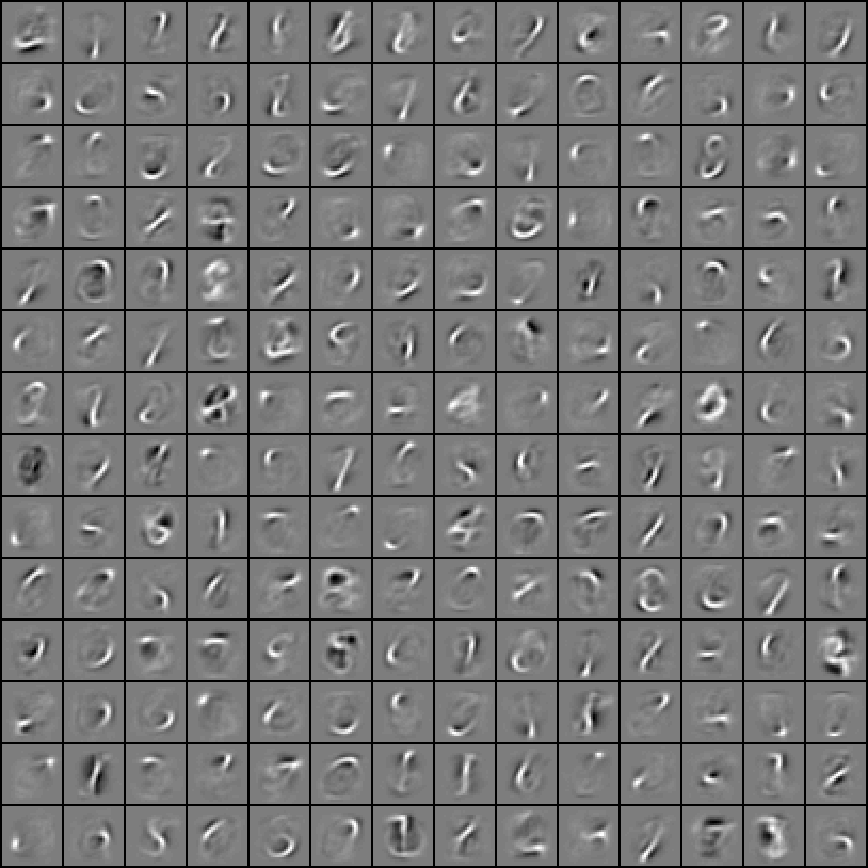
\includegraphics[width=0.6\textwidth]{figures/MnistVectorizationEx.png}
  %\caption{}\label{fig:step1}
\end{figure}

\cnt{If your parameters are improperly tuned, or if your implementation of the autoencoder is buggy, you may get one of the following images instead:}
    {}
    {}
\begin{figure}[ht] \centering
  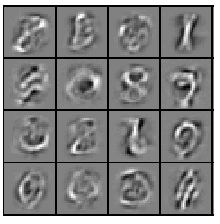
\includegraphics[width=0.4\textwidth]{figures/MNIST-false-bad-1.png}
  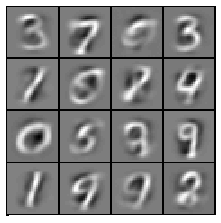
\includegraphics[width=0.4\textwidth]{figures/MNIST-false-bad-2.png}
  %\caption{}\label{fig:step1}
\end{figure}


\subsection{\cnt{Backpropagation vectorization hints}{反向传播矢量化提示}{}} \label{chp:backpropvechints}

Here, we give a few hints on how to vectorize the Backpropagation step. The hints here specifically build on our earlier description of how to vectorize a neural network(\ref{chp:neuralnetvec}).

Assume we have already implemented the vectorized forward propagation steps, so that the matrix-valued \texttt{z2, a2, z3} and \texttt{h} have already been computed. Here was our unvectorized implementation of \texttt{backprop}:
\begin{lstlisting}[language=matlab]
gradW1 = zeros(size(W1));
gradW2 = zeros(size(W2)); 
for i=1:m,
  delta3 = -(y(:,i) - h(:,i)) .* fprime(z3(:,i)); 
  delta2 = W2'*delta3(:,i) .* fprime(z2(:,i));
 
  gradW2 = gradW2 + delta3*a2(:,i)';
  gradW1 = gradW1 + delta2*a1(:,i)'; 
end;
\end{lstlisting}

Assume that we have implemented a version of \texttt{fprime(z)} that accepts matrix-valued inputs. We will use matrix-valued \texttt{delta3, delta2}. Here, \texttt{delta3} and \texttt{delta2} will have m columns, with one column per training example. We want to compute \texttt{delta3, delta2, gradW2} and \texttt{gradW1}.

Consider the computation for the matrix \texttt{delta3}, which can now be written:
\begin{lstlisting}[language=matlab]
for i=1:m, 
  delta3(:,i) = -(y(:,i) - h(:,i)) .* fprime(z3(:,i)); 
end;
\end{lstlisting}

Each iteration of the for loop computes one column of \texttt{delta3}. You should be able to find a single line of Matlab to compute \texttt{delta3} as a function of the matrices \texttt{y, h} and \texttt{z3}. This lets you compute \texttt{delta3}. Similarly, you should also be able to find a single line of code to compute the entire matrix \texttt{delta2}, as a function of \texttt{W2, delta3} (which is now a matrix), and \texttt{z2}.

Next, consider the computation for \texttt{gradW2}. We can now write this as:
\begin{lstlisting}[language=matlab]
gradW2 = zeros(size(W2));
for i=1:m, 
  gradW2 = gradW2 + delta3(:,i)*a2(:,i)';
end;
\end{lstlisting}

You should be able to find a single line of Matlab that replaces this for loop, and computes \texttt{gradW2} as a function of the matrices \texttt{delta3} and \texttt{a2}. If you're having trouble, take another look at the Logistic Regression Vectorization Example(\ref{chp:logisticvecexample}), which uses a related (but slightly different) vectorization step to get to the final implementation. Using a similar method, you will also be able to compute \texttt{gradW1} with a single line of code.

When you complete the derivation, you should be able to replace the unvectorized backpropagation code example above with just 4 lines of Matlab/Octave code. 


\clearpage
%# -*- coding: utf-8 -*-
%!TEX encoding = UTF-8 Unicode
%!TEX TS-program = xelatex
% vim:ts=4:sw=4
%
% 以上设定默认使用 XeLaTex 编译,并指定 Unicode 编码,供 TeXShop 自动识别

% Author: Yunhui Fu <yhfudev@gmail.com>
% License: Creative Commons (CC BY 4.0)

\section{\cnt{Preprocessing: PCA and Whitening}{预处理:主成分分析与白化}{}}

\subsection{\cnt{PCA}{主成分分析}{}}

\subsubsection{\cnt{Introduction}{引言}{}}

\cnt{Principal Components Analysis (PCA) is a dimensionality reduction algorithm that can be used to significantly speed up your unsupervised feature learning algorithm. More importantly, understanding PCA will enable us to later implement \emph{whitening}, which is an important pre-processing step for many algorithms.}
    {主成分分析(PCA)是一种能够极大提升无监督特征学习速度的数据降维算法。更重要的是,理解PCA算法,对实现白化算法有很大的帮助,很多算法都先用白化算法作预处理步骤。}
    {}

\cnt{Suppose you are training your algorithm on images. Then the input will be somewhat redundant, because the values of adjacent pixels in an image are highly correlated. Concretely, suppose we are training on $16 \times 16$ grayscale image patches. Then $x \in \Re^{256}$ are 256 dimensional vectors, with one feature $x_j$ corresponding to the intensity of each pixel. Because of the correlation between adjacent pixels, PCA will allow us to approximate the input with a much lower dimensional one, while incurring very little error.}
    {假设你使用图像来训练算法,因为图像中相邻的像素高度相关,输入数据是有一定冗余的。具体来说,假如我们正在训练的 $16 \times 16$ 灰度值图像,记为一个256维向量 $x \in \Re^{256}$,其中特征值 $x_j$ 对应每个像素的亮度值。由于相邻像素间的相关性,PCA算法可以将输入向量转换为一个维数低很多的近似向量,而且误差非常小。}
    {}

\subsubsection{\cnt{Example and Mathematical Background}{实例和数学背景}{}} \label{chp:examplemathbackground}

\cnt{For our running example, we will use a dataset $\{x^{(1)}, x^{(2)}, \ldots, x^{(m)}\}$ with $n=2$ dimensional inputs, so that $x^{(i)} \in \Re^2$. Suppose we want to reduce the data from 2 dimensions to 1. (In practice, we might want to reduce data from 256 to 50 dimensions, say; but using lower dimensional data in our example allows us to visualize the algorithms better.) Here is our dataset:}
    {在我们的实例中,使用的输入数据集表示为 $\{x^{(1)}, x^{(2)}, \ldots, x^{(m)}\}$,维度 $n=2$ 即 $x^{(i)} \in \Re^2$。假设我们想把数据从2维降到1维。(在实际应用中,我们也许需要把数据从256维降到50维;在这里使用低维数据,主要是为了更好地可视化算法的行为)。下图是我们的数据集:}
    {}

\begin{figure}[ht] \centering
  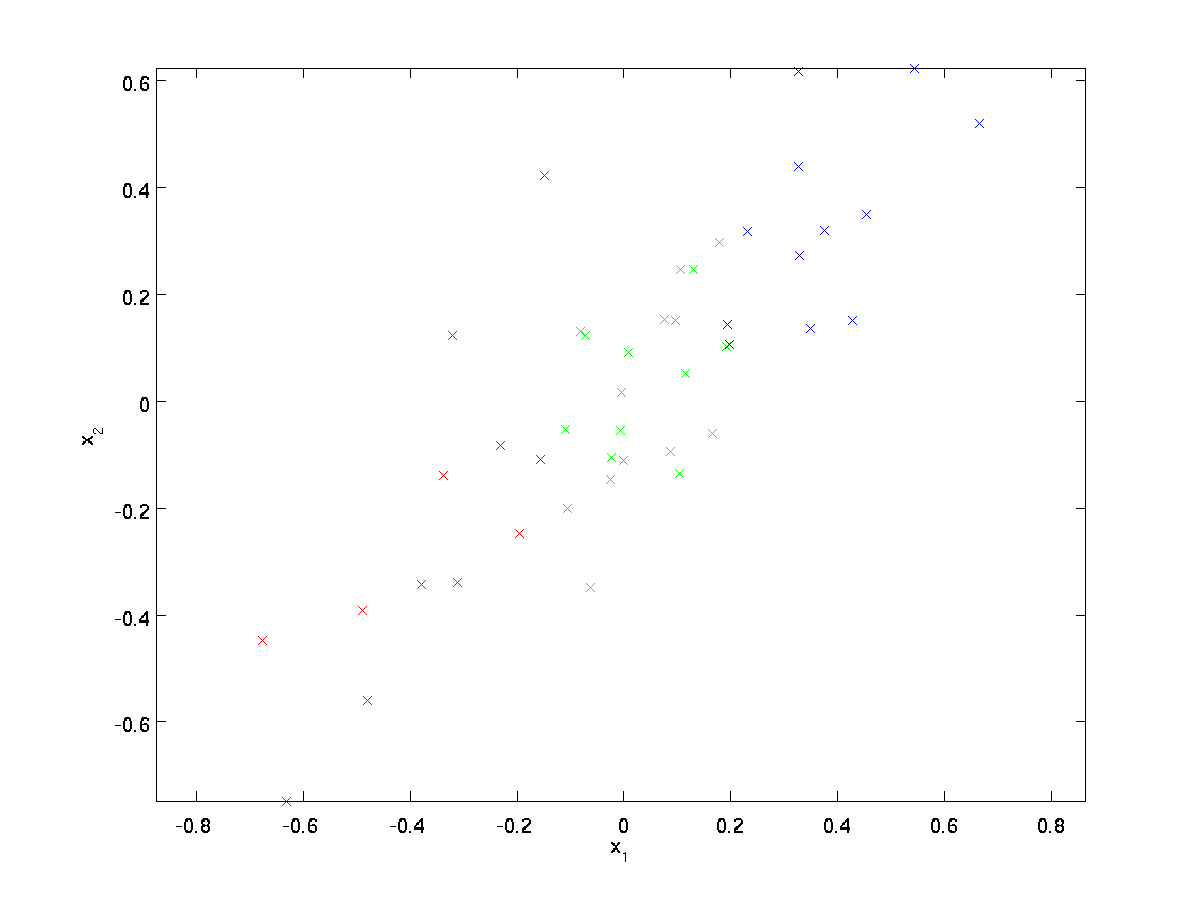
\includegraphics[width=0.8\textwidth]{figures/PCA-rawdata.png}
  %\caption{}\label{fig:step1}
\end{figure}

\cnt{This data has already been pre-processed so that each of the features $x_1$ and $x_2$ have about the same mean (zero) and variance.}
    {这些数据已经进行了预处理,使得每个特征 $x_1$ 和 $x_2$ 具有相同的均值(零)和方差。}
    {}

\cnt{For the purpose of illustration, we have also colored each of the points one of three colors, depending on their $x_1$ value; these colors are not used by the algorithm, and are for illustration only.}
    {为方便展示,根据 $x_1$ 值的大小,我们将每个点分别涂上了三种颜色之一,但该颜色并不用于算法而仅用于图解。}
    {}


\cnt{PCA will find a lower-dimensional subspace onto which to project our data. From visually examining the data, it appears that $u_1$ is the principal direction of variation of the data, and $u_2$ the secondary direction of variation:}
    {PCA算法将寻找一个低维空间来投影我们的数据。从下图中可以看出, $u_1$ 是数据变化的主方向,而 $u_2$ 是次方向。}
    {}

\begin{figure}[ht] \centering
  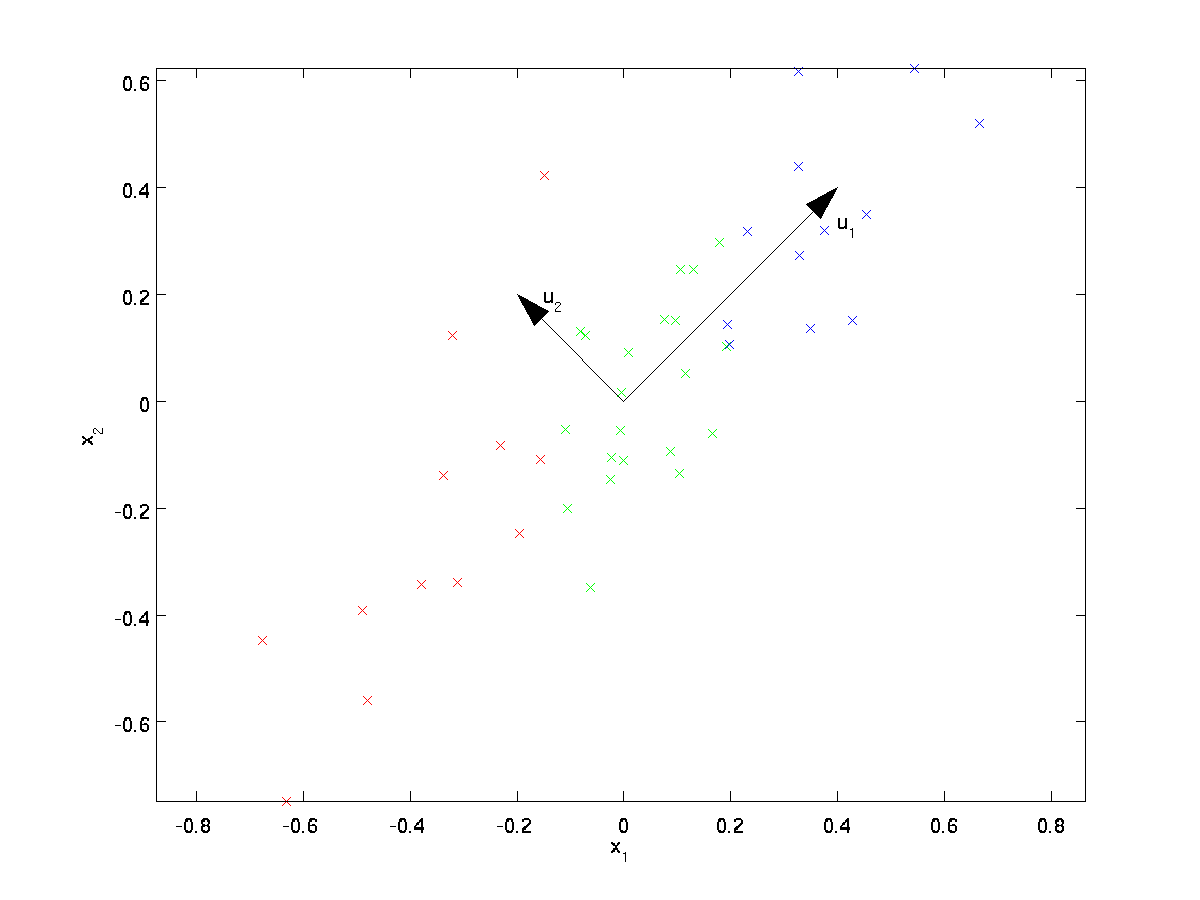
\includegraphics[width=0.8\textwidth]{figures/PCA-u1.png}
  %\caption{}\label{fig:step1}
\end{figure}


\cnt{I.e., the data varies much more in the direction $u_1$ than $u_2$. To more formally find the directions $u_1$ and $u_2$, we first compute the matrix $\Sigma$ as follows:}
    {也就是说,数据在 $u_1$ 方向上的变化要比在 $u_2$ 方向上大。为更形式化地找出方向 $u_1$ 和 $u_2$ ,我们首先计算出矩阵 $\Sigma$,如下所示:}
    {}

\begin{align} \Sigma = \frac{1}{m} \sum_{i=1}^m (x^{(i)})(x^{(i)})^T. \end{align} 

\cnt{If $x$ has zero mean, then $\Sigma$ is exactly the covariance matrix of $x$. (The symbol ``$\Sigma$", pronounced ``Sigma", is the standard notation for denoting the covariance matrix. Unfortunately it looks just like the summation symbol, as in $\sum_{i=1}^n i$; but these are two different things.)}
    {假设 $x$ 的均值为零,那么 $\Sigma$ 就是$x$的协方差矩阵。(符号 $\Sigma$,读``Sigma",是协方差矩阵的标准符号。虽然看起来与求和符号 $\sum_{i=1}^n i$ 比较像,但它们其实是两个不同的概念。)}
    {}


\cnt{It can then be shown that $u_1$ ---the principal direction of variation of the data---is the top (principal) eigenvector of $\Sigma$, and $u_2$ is the second eigenvector.}
    {可以证明,数据变化的主方向 $u_1$ 就是协方差矩阵 $\Sigma$ 的主特征向量,而 $u_2$ 是次特征向量。}
    {}

\cnt{Note: If you are interested in seeing a more formal mathematical derivation/justification of this result, see the CS229 (Machine Learning) lecture notes on PCA (link at bottom of this page). You won't need to do so to follow along this course, however.}
    {注:如果你对如何得到这个结果的具体数学推导过程感兴趣,可以参看CS229(机器学习)PCA部分的课件(链接在本页底部)。但如果仅仅是想跟上本课,可以不必如此。}
    {}


\cnt{You can use standard numerical linear algebra software to find these eigenvectors (see Implementation Notes). Concretely, let us compute the eigenvectors of $\Sigma$, and stack the eigenvectors in columns to form the matrix \texttt{U}:}
    {你可以通过标准的数值线性代数运算软件求得特征向量(见实现说明).我们先计算出协方差矩阵$\Sigma$的特征向量,按列排放,而组成矩阵\texttt{U}:}
    {}

\begin{align} U = \begin{bmatrix} | & | & & | \\ u_1 & u_2 & \cdots & u_n \\ | & | & & | \end{bmatrix} \end{align} 

\cnt{Here, $u_1$ is the principal eigenvector (corresponding to the largest eigenvalue), $u_2$ is the second eigenvector, and so on. Also, let $\lambda_1, \lambda_2, \ldots, \lambda_n$ be the corresponding eigenvalues.}
    {此处, $u_1$ 是主特征向量(对应最大的特征值), $u_2$ 是次特征向量。以此类推,另记 $\lambda_1, \lambda_2, \ldots, \lambda_n$ 为相应的特征值。}
    {}


\cnt{The vectors $u_1$ and $u_2$ in our example form a new basis in which we can represent the data. Concretely, let $x \in \Re^2$ be some training example. Then $u_1^Tx$ is the length (magnitude) of the projection of $x$ onto the vector $u_1$.}
    {在本例中,向量 $u_1$ 和 $u_2$ 构成了一个新基,可以用来表示数据。令 $x \in \Re^2$ 为训练样本,那么 $u_1^Tx$ 就是样本点 $x$ 在维度 $u_1$ 上的投影的长度(幅值)。}
    {}

\cnt{Similarly, $u_2^Tx$ is the magnitude of $x$ projected onto the vector $u_2$.}
    {同样的, $u_2^Tx$ 是 $x$ 投影到 $u_2$ 维度上的幅值。}
    {}


\subsubsection{\cnt{Rotating the Data}{旋转数据}{}} \label{chp:rotatedatapca}

\cnt{Thus, we can represent $x$ in the $(u_1, u_2)$-basis by computing}
    {至此,我们可以把 $x$ 用 $(u_1, u_2)$ 基表达为:}
    {}
\begin{align} x_{\rm rot} = U^Tx = \begin{bmatrix} u_1^Tx \\ u_2^Tx \end{bmatrix} \end{align}

\cnt{(The subscript ``rot" comes from the observation that this corresponds to a rotation (and possibly reflection) of the original data.) Lets take the entire training set, and compute $x_{\rm rot}^{(i)} = U^Tx^{(i)}$ for every $i$. Plotting this transformed data $x_{\rm rot}$, we get:}
    {(下标“rot”来源于单词“rotation”,意指这是原数据经过旋转(也可以说成映射)后得到的结果)对数据集中的每个样本 $i$ 分别进行旋转: $x_{\rm rot}^{(i)} = U^Tx^{(i)}$ for every $i$,然后把变换后的数据 $x_{\rm rot}$ 显示在坐标图上,可得:}
    {}

\begin{figure}[ht] \centering
  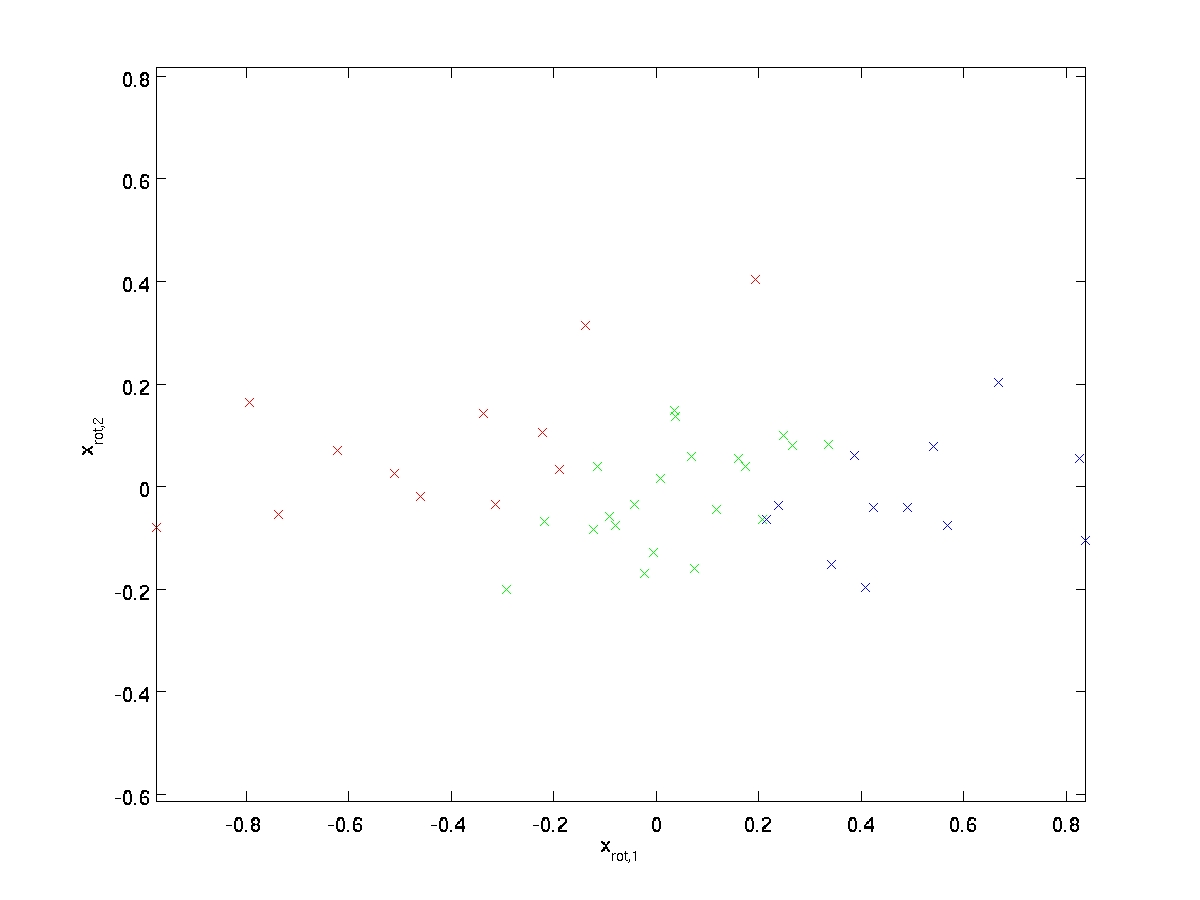
\includegraphics[width=0.8\textwidth]{figures/PCA-rotated.png}
  \caption{}\label{fig:pcarotated}
\end{figure}

\cnt{This is the training set rotated into the $u_1, u_2$ basis. In the general case, $U^Tx$ will be the training set rotated into the basis $u_1, u_2, \ldots, u_n$.}
    {这就是把训练数据集旋转到 $u_1, u_2$ 基后的结果。一般而言,运算 $U^Tx$ 表示旋转到基 $u_1, u_2, \ldots, u_n$ 之上的训练数据。}
    {}

\cnt{One of the properties of $U$ is that it is an ``orthogonal" matrix, which means that it satisfies $U^TU = UU^T = I$. So if you ever need to go from the rotated vectors $x_{\rm rot}$ back to the original data $x$, you can compute}
    {矩阵 $U$ 有正交性,即满足 $U^TU = UU^T = I$,所以若想将旋转后的向量 $x_{\rm rot}$ 还原为原始数据 $x$,将其左乘矩阵$U$ 即可: $x=U x_{\rm rot}$, 验算一下: $U x_{\rm rot} = UU^T x = x$.}
    {}
    \begin{align} x = U x_{\rm rot} , \end{align} 
\cnt{because $U x_{\rm rot} = UU^T x = x$.}
    {}
    {}



\subsubsection{\cnt{Reducing the Data Dimension}{数据降维}{}}

\cnt{We see that the principal direction of variation of the data is the first dimension $x_{{\rm rot},1}$ of this rotated data. Thus, if we want to reduce this data to one dimension, we can set}
    {数据的主方向就是旋转数据的第一维 $x_{{\rm rot},1}$。因此,若想把这数据降到一维,可令:}
    {}
\begin{align} \tilde{x}^{(i)} = x_{{\rm rot},1}^{(i)} = u_1^Tx^{(i)} \in \Re. \end{align}

\cnt{More generally, if $x \in \Re^n$ and we want to reduce it to a $k$ dimensional representation $\tilde{x} \in \Re^k$ (where $k < n$), we would take the first $k$ components of $x_{\rm rot}$, which correspond to the top $k$ directions of variation.}
    {更一般的,假如想把数据 $x \in \Re^n$ 降到 $k$ 维表示 $\tilde{x} \in \Re^k$ (令 $k < n$),只需选取 $x_{\rm rot}$ 的前 $k$ 个成分,分别对应前 $k$ 个数据变化的主方向。}
    {}

\cnt{Another way of explaining PCA is that $x_{\rm rot}$ is an $n$ dimensional vector, where the first few components are likely to be large (e.g., in our example, we saw that $x_{{\rm rot},1}^{(i)} = u_1^Tx^{(i)}$ takes reasonably large values for most examples $i$), and the later components are likely to be small (e.g., in our example, $x_{{\rm rot},2}^{(i)} = u_2^Tx^{(i)}$ was more likely to be small).}
    {PCA的另外一种解释是:$x_{\rm rot}$ 是一个 $n$ 维向量,其中前几个成分可能比较大(例如,上例中大部分样本第一个成分 $x_{{\rm rot},1}^{(i)} = u_1^Tx^{(i)}$ 的取值相对较大),而后面成分可能会比较小(例如,上例中大部分样本的 $x_{{\rm rot},2}^{(i)} = u_2^Tx^{(i)}$ 较小)。}
    {}

\cnt{What PCA does it it drops the the later (smaller) components of $x_{\rm rot}$, and just approximates them with 0's. Concretely, our definition of $\tilde{x}$ can also be arrived at by using an approximation to $x_{{\rm rot}}$ where all but the first $k$ components are zeros. In other words, we have:}
    {PCA算法做的其实就是丢弃 $x_{\rm rot}$ 中后面(取值较小)的成分,就是将这些成分的值近似为零。具体的说,设 $\tilde{x}$ 是 $x_{{\rm rot}}$ 的近似表示,那么将 $x_{{\rm rot}}$ 除了前 $k$ 个成分外,其余全赋值为零,就得到:}
    {}

\begin{align} \tilde{x} = \begin{bmatrix} x_{{\rm rot},1} \\ \vdots \\ x_{{\rm rot},k} \\ 0 \\ \vdots \\ 0 \\ \end{bmatrix} \approx \begin{bmatrix} x_{{\rm rot},1} \\ \vdots \\ x_{{\rm rot},k} \\ x_{{\rm rot},k+1} \\ \vdots \\ x_{{\rm rot},n} \end{bmatrix} = x_{\rm rot} \end{align}

\cnt{In our example, this gives us the following plot of $\tilde{x}$ (using $n=2, k=1$):}
    {在本例中,可得 $\tilde{x}$ 的点图如下(取 $n=2, k=1$ ):}
    {}

\begin{figure}[ht] \centering
  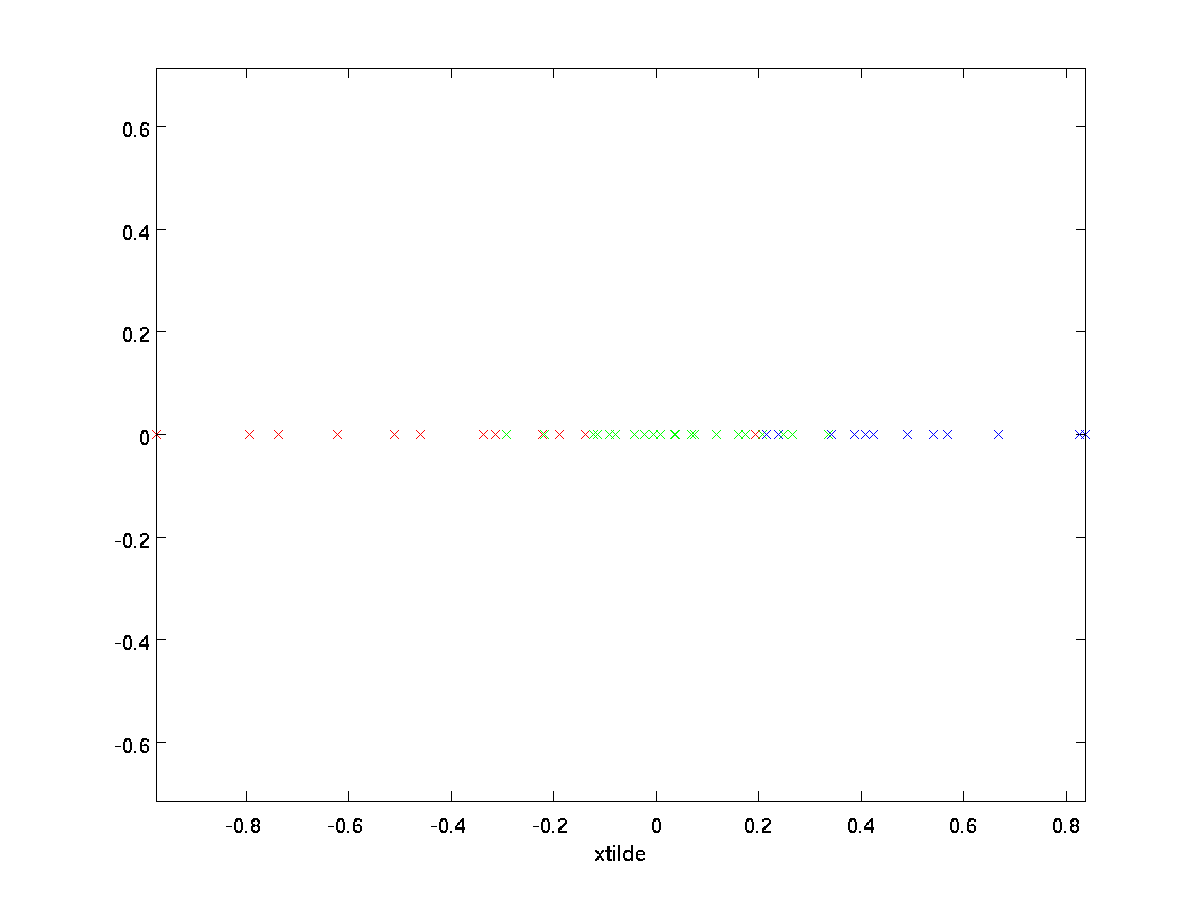
\includegraphics[width=0.8\textwidth]{figures/PCA-xtilde.png}
  %\caption{}\label{fig:step1}
\end{figure}

\cnt{However, since the final $n-k$ components of $\tilde{x}$ as defined above would always be zero, there is no need to keep these zeros around, and so we define $\tilde{x}$ as a $k$-dimensional vector with just the first $k$ (non-zero) components.}
    {然而,由于上面 $\tilde{x}$ 的后 $n-k$ 项均为零,没必要把这些零项保留下来。所以,我们仅用前 $k$ 个(非零)成分来定义 $k$ 维向量 $\tilde{x}$。}
    {}

\cnt{This also explains why we wanted to express our data in the $u_1, u_2, \ldots, u_n$ basis: Deciding which components to keep becomes just keeping the top $k$ components. When we do this, we also say that we are ``retaining the top $k$ PCA (or principal) components."}
    {这也解释了我们为什么会以 $u_1, u_2, \ldots, u_n$ 为基来表示数据:要决定保留哪些成分变得很简单,只需取前 $k$ 个成分即可。这时也可以说,我们“保留了前 $k$ 个PCA(主)成分”。}
    {}


\subsubsection{\cnt{Recovering an Approximation of the Data}{还原近似数据}{}}

\cnt{Now, $\tilde{x} \in \Re^k$ is a lower-dimensional, ``compressed" representation of the original $x \in \Re^n$. Given $\tilde{x}$, how can we recover an approximation $\hat{x}$ to the original value of $x$? From an earlier section(\ref{chp:rotatedatapca}), we know that $x = U x_{\rm rot}$. Further, we can think of $\tilde{x}$ as an approximation to $x_{\rm rot}$, where we have set the last $n-k$ components to zeros. Thus, given $\tilde{x} \in \Re^k$, we can pad it out with $n-k$ zeros to get our approximation to $x_{\rm rot} \in \Re^n$. Finally, we pre-multiply by $U$ to get our approximation to $x$. Concretely, we get}
    {现在,我们得到了原始数据 $x \in \Re^n$ 的低维“压缩”表征量 $\tilde{x} \in \Re^k$, 反过来,如果给定 $\tilde{x}$,我们应如何还原原始数据 $x$ 呢?查看以往章节(\ref{chp:rotatedatapca})可知,要转换回来,只需 $x = U x_{\rm rot}$ 即可。进一步,我们把 $\tilde{x}$ 看作将 $x_{\rm rot}$ 的最后 $n-k$ 个元素被置0所得的近似表示,因此如果给定 $\tilde{x} \in \Re^k$,可以通过在其末尾添加 $n-k$ 个0来得到对 $x_{\rm rot} \in \Re^n$ 的近似,最后,左乘 $U$ 便可近似还原出原数据 $x$。具体来说,计算如下:}
    {}
\begin{align} \hat{x} = U \begin{bmatrix} \tilde{x}_1 \\ \vdots \\ \tilde{x}_k \\ 0 \\ \vdots \\ 0 \end{bmatrix} = \sum_{i=1}^k u_i \tilde{x}_i. \end{align}

\cnt{The final equality above comes from the definition of $U$ given earlier(\ref{chp:examplemathbackground}). (In a practical implementation, we wouldn't actually zero pad $\tilde{x}$ and then multiply by $U$, since that would mean multiplying a lot of things by zeros; instead, we'd just multiply $\tilde{x} \in \Re^k$ with the first $k$ columns of $U$ as in the final expression above.) Applying this to our dataset, we get the following plot for $\hat{x}$:}
    {上面的等式基于先前(\ref{chp:examplemathbackground})对 $U$ 的定义。在实现时,我们实际上并不先给 $\tilde{x}$ 填0然后再左乘 $U$,因为这意味着大量的乘0运算。我们可用 $\tilde{x} \in \Re^k$ 来与 $U$ 的前 $k$ 列相乘,即上式中最右项,来达到同样的目的。将该算法应用于本例中的数据集,可得如下关于重构数据 $\hat{x}$ 的点图:}
    {}

\begin{figure}[ht] \centering
  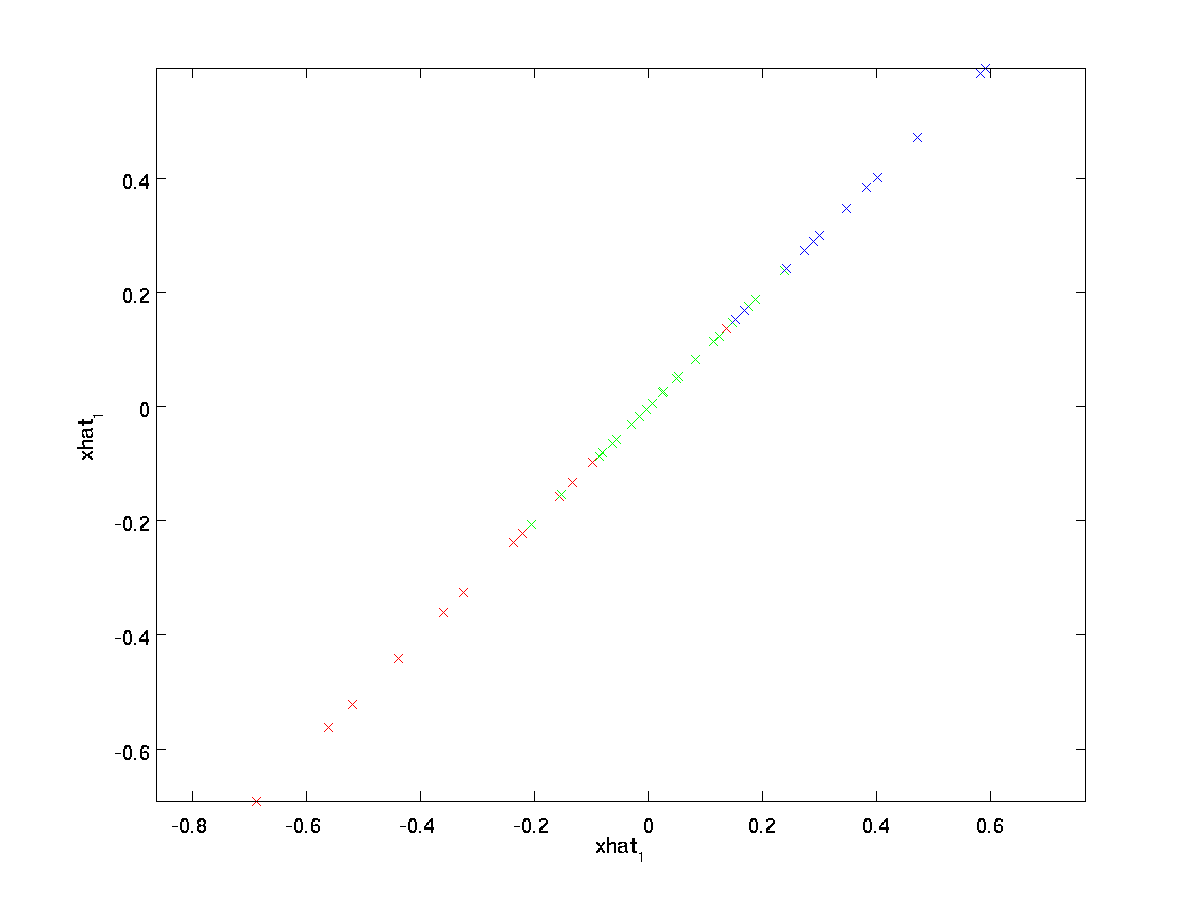
\includegraphics[width=0.8\textwidth]{figures/PCA-xhat.png}
  %\caption{}\label{fig:step1}
\end{figure}

\cnt{We are thus using a 1 dimensional approximation to the original dataset.}
    {由图可见,我们得到的是对原始数据集的一维近似重构。}
    {}

\cnt{If you are training an autoencoder or other unsupervised feature learning algorithm, the running time of your algorithm will depend on the dimension of the input. If you feed $\tilde{x} \in \Re^k$ into your learning algorithm instead of $x$, then you'll be training on a lower-dimensional input, and thus your algorithm might run significantly faster. For many datasets, the lower dimensional $\tilde{x}$ representation can be an extremely good approximation to the original, and using PCA this way can significantly speed up your algorithm while introducing very little approximation error.}
    {在训练自动编码器或其它无监督特征学习算法时,算法运行时间将依赖于输入数据的维数。若用 $\tilde{x} \in \Re^k$ 取代 $x$ 作为输入数据,那么算法就可使用低维数据进行训练,运行速度将显著加快。对于很多数据集来说,低维表征量 $\tilde{x}$ 是原数据集的极佳近似,因此在这些场合使用PCA是很合适的,它引入的近似误差的很小,却可显著地提高你算法的运行速度。}
    {}

\subsubsection{\cnt{Number of components to retain}{选择主成分个数}{}} \label{chp:pcaselectnum}

\cnt{How do we set $k$; i.e., how many PCA components should we retain? In our simple 2 dimensional example, it seemed natural to retain 1 out of the 2 components, but for higher dimensional data, this decision is less trivial. If $k$ is too large, then we won't be compressing the data much; in the limit of $k=n$, then we're just using the original data (but rotated into a different basis). Conversely, if $k$ is too small, then we might be using a very bad approximation to the data.}
    {我们该如何选择 $k$,即保留多少个PCA主成分?在上面这个简单的二维实验中,保留第一个成分看起来是自然的选择。对于高维数据来说,做这个决定就没那么简单:如果 $k$ 过大,数据压缩率不高,在极限情况 $k=n$ 时,等于是在使用原始数据(只是旋转投射到了不同的基);相反地,如果 $k$ 过小,那数据的近似误差太太。}
    {}

\cnt{To decide how to set $k$, we will usually look at the \emph{percentage of variance retained} for different values of $k$. Concretely, if $k=n$, then we have an exact approximation to the data, and we say that 100\% of the variance is retained. I.e., all of the variation of the original data is retained. Conversely, if $k=0$, then we are approximating all the data with the zero vector, and thus 0\% of the variance is retained.}
    {决定 $k$ 值时,我们通常会考虑不同 $k$ 值\emph{可保留的方差百分比}。具体来说,如果 $k=n$,那么我们得到的是对数据的完美近似,也就是保留了100\%的方差,即原始数据的所有变化都被保留下来;相反,如果 $k=0$,那等于是使用零向量来逼近输入数据,也就是只有0\%的方差被保留下来。}
    {}


\cnt{More generally, let $\lambda_1, \lambda_2, \ldots, \lambda_n$ be the eigenvalues of $\Sigma$ (sorted in decreasing order), so that $\lambda_j$ is the eigenvalue corresponding to the eigenvector $u_j$. Then if we retain $k$ principal components, the percentage of variance retained is given by:}
    {一般而言,设 $\lambda_1, \lambda_2, \ldots, \lambda_n$ 表示 $\Sigma$ 的特征值(按由大到小顺序排列),使得 $\lambda_j$ 为对应于特征向量 $u_j$ 的特征值。那么如果我们保留前 $k$ 个成分,则保留的方差百分比可计算为:}
    {}
\begin{align} \frac{\sum_{j=1}^k \lambda_j}{\sum_{j=1}^n \lambda_j}. \end{align}


\cnt{In our simple 2D example above, $\lambda_1 = 7.29$, and $\lambda_2 = 0.69$. Thus, by keeping only $k=1$ principal components, we retained $7.29/(7.29+0.69) = 0.913$, or 91.3\% of the variance.}
    {在上面简单的二维实验中,$\lambda_1 = 7.29, \lambda_2 = 0.69$。因此,如果保留 $k=1$ 个主成分,等于我们保留了 $7.29/(7.29+0.69) = 0.913$,即91.3\%的方差。}
    {}

\cnt{A more formal definition of percentage of variance retained is beyond the scope of these notes. However, it is possible to show that $\lambda_j = \sum_{i=1}^m x_{{\rm rot},j}^2$. Thus, if $\lambda_j \approx 0$, that shows that $x_{{\rm rot},j}$ is usually near 0 anyway, and we lose relatively little by approximating it with a constant 0. This also explains why we retain the top principal components (corresponding to the larger values of $\lambda_j$) instead of the bottom ones. The top principal components $x_{{\rm rot},j}$ are the ones that're more variable and that take on larger values, and for which we would incur a greater approximation error if we were to set them to zero.}
    {对保留方差的百分比进行更正式的定义已超出了本教程的范围,但很容易证明,$\lambda_j = \sum_{i=1}^m x_{{\rm rot},j}^2$ 。因此,如果 $\lambda_j \approx 0$,则说明 $x_{{\rm rot},j}$ 也就基本上接近于0,所以用0来近似它并不会产生多大损失。这也解释了为什么要保留前面的主成分(对应的 $\lambda_j$ 值较大)而不是末尾的那些。 这些前面的主成分 $x_{{\rm rot},j}$ 变化性更大,取值也更大,如果将其设为0势必引入较大的近似误差。}
    {}

\cnt{In the case of images, one common heuristic is to choose $k$ so as to retain 99\% of the variance. In other words, we pick the smallest value of $k$ that satisfies}
    {以处理图像数据为例,一个惯常的经验法则是选择 $k$ 以保留99\%的方差,换句话说,我们选取满足以下条件的最小 $k$ 值:}
    {}
\begin{align} \frac{\sum_{j=1}^k \lambda_j}{\sum_{j=1}^n \lambda_j} \geq 0.99. \end{align}

\cnt{Depending on the application, if you are willing to incur some additional error, values in the 90-98\% range are also sometimes used. When you describe to others how you applied PCA, saying that you chose $k$ to retain 95\% of the variance will also be a much more easily interpretable description than saying that you retained 120 (or whatever other number of) components.}
    {对其它应用,如不介意引入稍大的误差,有时也保留90-98\%的方差范围。若向他人介绍PCA算法详情,告诉他们你选择的 $k$ 保留了95\%的方差,比告诉他们你保留了前120个(或任意某个数字)主成分更好理解。 }
    {}

\subsubsection{\cnt{PCA on Images}{对图像数据应用PCA算法}{}}

\cnt{For PCA to work, usually we want each of the features $x_1, x_2, \ldots, x_n$ to have a similar range of values to the others (and to have a mean close to zero). If you've used PCA on other applications before, you may therefore have separately pre-processed each feature to have zero mean and unit variance, by separately estimating the mean and variance of each feature $x_j$. However, this isn't the pre-processing that we will apply to most types of images. Specifically, suppose we are training our algorithm on natural images, so that $x_j$ is the value of pixel $j$. By ``natural images," we informally mean the type of image that a typical animal or person might see over their lifetime.}
    {为使PCA算法能有效工作,通常我们希望所有的特征 $x_1, x_2, \ldots, x_n$ 都有相似的取值范围(并且均值接近于0)。如果你曾在其它应用中使用过PCA算法,你可能知道有必要单独对每个特征做预处理,即通过估算每个特征 $x_j$ 的均值和方差,而后将其取值范围规整化为零均值和单位方差。但是,对于大部分图像类型,我们却不需要进行这样的预处理。假定我们将在自然图像上训练算法,此时特征 $x_j$ 代表的是像素 $j$ 的值。所谓“自然图像”,不严格的说,是指人或动物在他们一生中所见的那种图像。}
    {}

\cnt{Note: Usually we use images of outdoor scenes with grass, trees, etc., and cut out small (say $16 \times 16$) image patches randomly from these to train the algorithm. But in practice most feature learning algorithms are extremely robust to the exact type of image it is trained on, so most images taken with a normal camera, so long as they aren't excessively blurry or have strange artifacts, should work.}
    {注:通常我们选取含草木等内容的户外场景图片,然后从中随机截取小图像块(如$16 \times 16$像素)来训练算法。在实践中我们发现,大多数特征学习算法对训练图片的确切类型并不敏感,所以大多数用普通照相机拍摄的图片,只要不是特别的模糊或带有非常奇怪的人工痕迹,都可以使用。}
    {}

\cnt{When training on natural images, it makes little sense to estimate a separate mean and variance for each pixel, because the statistics in one part of the image should (theoretically) be the same as any other. This property of images is called \emph{stationarity}.}
    {在自然图像上进行训练时,对每一个像素单独估计均值和方差意义不大,因为(理论上)图像任一部分的统计性质都应该和其它部分相同,图像的这种特性被称作\emph{平稳性}(stationarity)。}
    {}

\cnt{In detail, in order for PCA to work well, informally we require that (i) The features have approximately zero mean, and (ii) The different features have similar variances to each other. With natural images, (ii) is already satisfied even without variance normalization, and so we won't perform any variance normalization. (If you are training on audio data---say, on spectrograms---or on text data---say, bag-of-word vectors---we will usually not perform variance normalization either.) In fact, PCA is invariant to the scaling of the data, and will return the same eigenvectors regardless of the scaling of the input. More formally, if you multiply each feature vector $x$ by some positive number (thus scaling every feature in every training example by the same number), PCA's output eigenvectors will not change.}
    {具体而言,为使PCA算法正常工作,我们通常需要满足以下要求:(1)特征的均值大致为0;(2)不同特征的方差值彼此相似。对于自然图片,即使不进行方差归一化操作,条件(2)也自然满足,故而我们不再进行任何方差归一化操作(对音频数据,如声谱,或文本数据,如词袋向量,我们通常也不进行方差归一化)。实际上,PCA算法对输入数据具有缩放不变性,无论输入数据的值被如何放大(或缩小),返回的特征向量都不改变。更正式的说:如果将每个特征向量 $x$ 都乘以某个正数(即所有特征量被放大或缩小相同的倍数),PCA的输出特征向量都将不会发生变化。}
    {}

\cnt{So, we won't use variance normalization. The only normalization we need to perform then is mean normalization, to ensure that the features have a mean around zero. Depending on the application, very often we are not interested in how bright the overall input image is. For example, in object recognition tasks, the overall brightness of the image doesn't affect what objects there are in the image. More formally, we are not interested in the mean intensity value of an image patch; thus, we can subtract out this value, as a form of mean normalization.}
    {既然我们不做方差归一化,唯一还需进行的规整化操作就是均值规整化,其目的是保证所有特征的均值都在0附近。根据应用,在大多数情况下,我们并不关注所输入图像的整体明亮程度。比如在对象识别任务中,图像的整体明亮程度并不会影响图像中存在的是什么物体。更为正式地说,我们对图像块的平均亮度值不感兴趣,所以可以减去这个值来进行均值规整化。}
    {}

\cnt{Concretely, if $x^{(i)} \in \Re^{n}$ are the (grayscale) intensity values of a $16 \times 16$ image patch ($n=256$), we might normalize the intensity of each image $x^{(i)}$ as follows:}
    {具体的步骤是,如果 $x^{(i)} \in \Re^{n}$ 代表$16 \times 16$的图像块的亮度(灰度)值( $n=256$ ),可用如下算法来对每幅图像进行零均值化操作:}
    {}
$$
\mu^{(i)} := \frac{1}{n} \sum_{j=1}^n x^{(i)}_j
$$
$$
x^{(i)}_j := x^{(i)}_j - \mu^{(i)}, {\rm ~ for all ~} j
$$

\cnt{Note that the two steps above are done separately for each image $x^{(i)}$, and that $\mu^{(i)}$ here is the mean intensity of the image $x^{(i)}$. In particular, this is not the same thing as estimating a mean value separately for each pixel $x_j$.}
    {请注意:1)对每个输入图像块 $x^{(i)}$ 都要单独执行上面两个步骤,2)这里的 $\mu^{(i)}$ 是指图像块 $x^{(i)}$ 的平均亮度值。尤其需要注意的是,这和为每个像素 $x_j$ 单独估算均值是两个完全不同的概念。}
    {}

\cnt{If you are training your algorithm on images other than natural images (for example, images of handwritten characters, or images of single isolated objects centered against a white background), other types of normalization might be worth considering, and the best choice may be application dependent. But when training on natural images, using the per-image mean normalization method as given in the equations above would be a reasonable default.}
    {如果你处理的图像并非自然图像(比如,手写文字,或者白背景正中摆放单独物体),其他规整化操作就值得考虑了,而哪种做法最合适也取决于具体应用场合。但对自然图像而言,对每幅图像进行上述的零均值规整化,是默认而合理的处理。}
    {}

\subsubsection{\cnt{References}{参考文献}{}}
\url{http://cs229.stanford.edu/}




\subsection{\cnt{Whitening}{白化}{}} \label{chp:whitening}

\subsubsection{\cnt{Introduction}{介绍}{}}

\cnt{We have used PCA to reduce the dimension of the data. There is a closely related preprocessing step called \emph{whitening} (or, in some other literatures, \emph{sphering}) which is needed for some algorithms. If we are training on images, the raw input is redundant, since adjacent pixel values are highly correlated. The goal of whitening is to make the input less redundant; more formally, our desiderata are that our learning algorithms sees a training input where (i) the features are less correlated with each other, and (ii) the features all have the same variance.}
    {我们已经了解了如何使用PCA降低数据维度。在一些算法中还需要一个与之相关的预处理步骤,这个预处理过程称为\emph{白化}(一些文献中也叫 \emph{sphering})。举例来说,假设训练数据是图像,由于图像中相邻像素之间具有很强的相关性,所以用于训练时输入是冗余的。白化的目的就是降低输入的冗余性;更正式的说,我们希望通过白化过程使得学习算法的输入具有如下性质:(i)特征之间相关性较低;(ii)所有特征具有相同的方差。}
    {}

\subsubsection{\cnt{2D example}{2D 的例子}{}}

\cnt{We will first describe whitening using our previous 2D example. We will then describe how this can be combined with smoothing, and finally how to combine this with PCA.}
    {下面我们先用前文的2D例子描述白化的主要思想,然后分别介绍如何将白化与平滑和PCA相结合。}
    {}

\cnt{How can we make our input features uncorrelated with each other? We had already done this when computing $x_{\rm rot}^{(i)} = U^Tx^{(i)}$. Repeating our previous figure, our plot for $x_{\rm rot}$ was: }
    {如何消除输入特征之间的相关性? 在前文计算 $x_{\rm rot}^{(i)} = U^Tx^{(i)}$ 时实际上已经消除了输入特征$x^{(i)}$之间的相关性。得到的新特征 $x_{\rm rot}$ 的分布如 图 \ref{fig:pcarotated} 所示:}
    {}

\begin{figure}[ht] \centering
  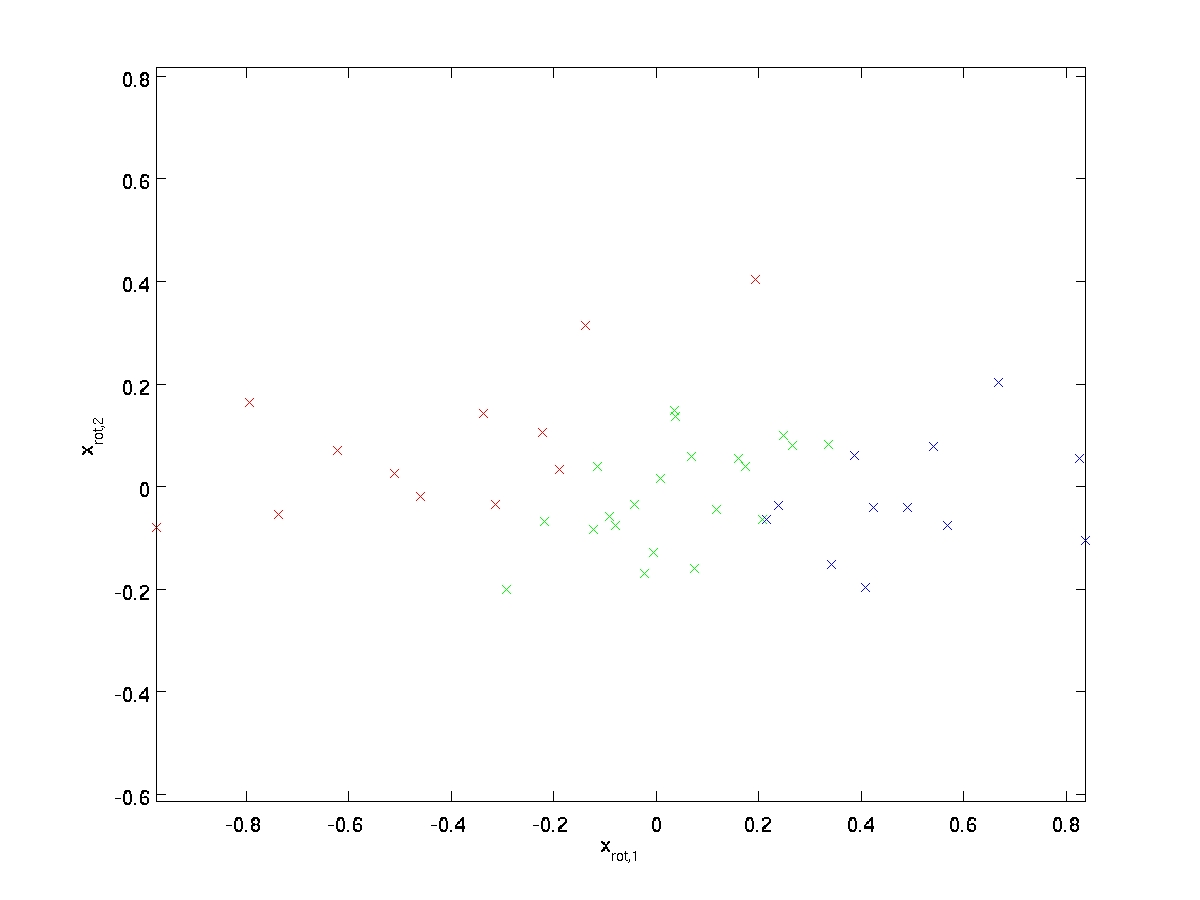
\includegraphics[width=0.8\textwidth]{figures/PCA-rotated.png}
  \caption{}\label{fig:pcarotated2}
\end{figure}

\cnt{The covariance matrix of this data is given by:}
    {这个数据的协方差矩阵如下:}
    {}
\begin{align} \begin{bmatrix} 7.29 & 0 \\ 0 & 0.69 \end{bmatrix}. \end{align}

\cnt{(Note: Technically, many of the statements in this section about the ``covariance" will be true only if the data has zero mean. In the rest of this section, we will take this assumption as implicit in our statements. However, even if the data's mean isn't exactly zero, the intuitions we're presenting here still hold true, and so this isn't something that you should worry about.)}
    {(注: 严格地讲, 这部分许多关于“协方差”的陈述仅当数据均值为0时成立。下文的论述都隐式地假定这一条件成立。不过即使数据均值不为0,下文的说法仍然成立,所以你无需担心这个。)}
    {}

\cnt{It is no accident that the diagonal values are $\lambda_1$ and $\lambda_2$. Further, the off-diagonal entries are zero; thus, $x_{{\rm rot},1}$ and $x_{{\rm rot},2}$ are uncorrelated, satisfying one of our desiderata for whitened data (that the features be less correlated).}
    {$x_{\rm rot}$ 协方差矩阵对角元素的值为 $\lambda_1$ 和 $\lambda_2$ 绝非偶然。并且非对角元素值为0; 因此, $x_{{\rm rot},1}$ 和 $x_{{\rm rot},2}$ 是不相关的, 满足我们对白化结果的第一个要求 (特征间相关性降低)。}
    {}

\cnt{To make each of our input features have unit variance, we can simply rescale each feature $x_{{\rm rot},i}$ by $1/\sqrt{\lambda_i}$. Concretely, we define our whitened data $x_{{\rm PCAwhite}} \in \Re^n$ as follows:}
    {为了使每个输入特征具有单位方差,我们可以直接使用 $1/\sqrt{\lambda_i}$ 作为缩放因子来缩放每个特征 $x_{{\rm rot},i}$。具体地,我们定义白化后的数据 $x_{{\rm PCAwhite}} \in \Re^n$ 如下:}
    {}

\begin{align} x_{{\rm PCAwhite},i} = \frac{x_{{\rm rot},i} }{\sqrt{\lambda_i}}. \end{align}

\cnt{Plotting $x_{{\rm PCAwhite}}$, we get:}
    {绘制出 $x_{{\rm PCAwhite}}$,我们得到:}
    {}

\begin{figure}[ht] \centering
  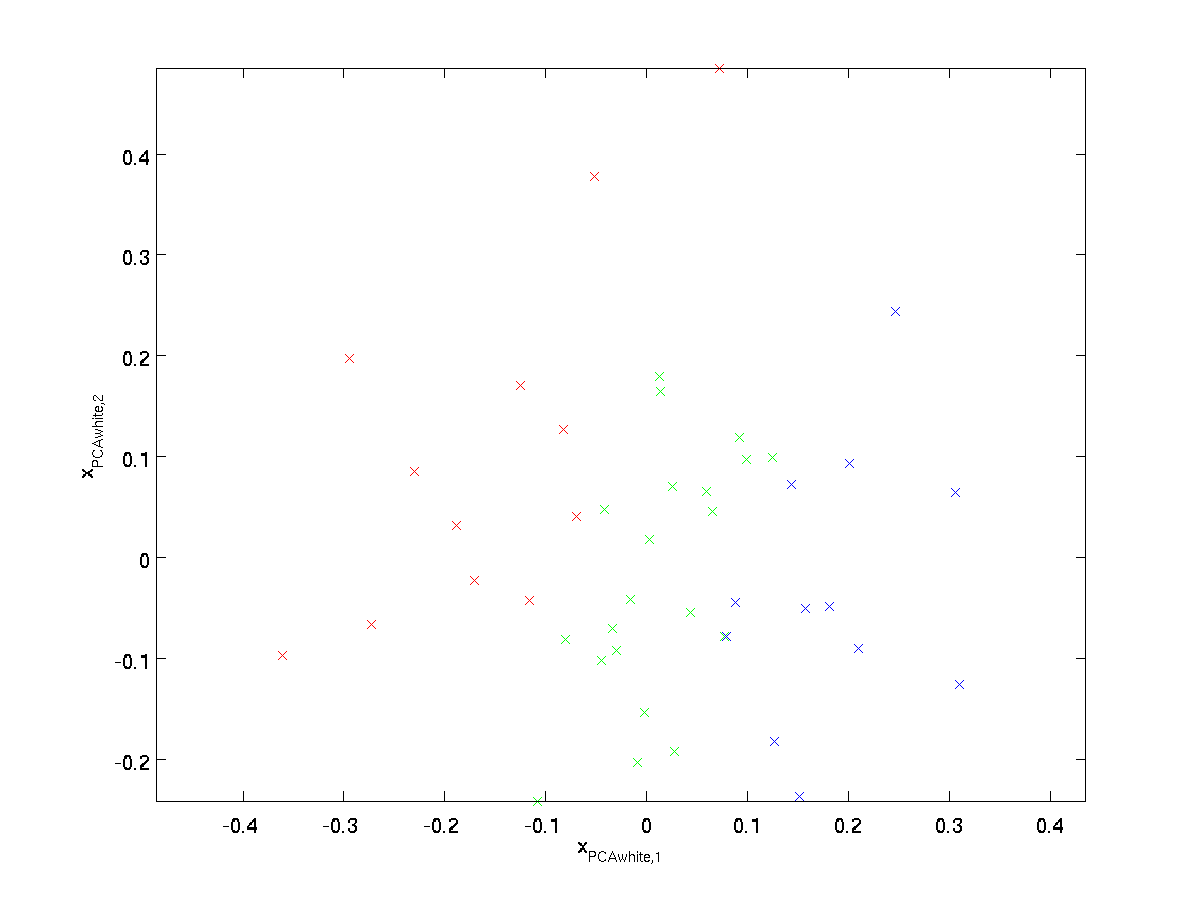
\includegraphics[width=0.8\textwidth]{figures/PCA-whitened.png}
  \caption{}\label{fig:pcarotated2}
\end{figure}

\cnt{This data now has covariance equal to the identity matrix $I$. We say that $x_{{\rm PCAwhite}}$ is our \emph{PCA whitened} version of the data: The different components of $x_{{\rm PCAwhite}}$ are uncorrelated and have unit variance.}
    {这些数据现在的协方差矩阵为单位矩阵 $I$。我们说,$x_{{\rm PCAwhite}}$ 是数据经过\emph{PCA白化}后的版本: $x_{{\rm PCAwhite}}$ 中不同的特征之间不相关并且具有单位方差。}
    {}

\cnt{\emph{Whitening combined with dimensionality reduction}. If you want to have data that is whitened and which is lower dimensional than the original input, you can also optionally keep only the top $k$ components of $x_{{\rm PCAwhite}}$. When we combine PCA whitening with regularization (described later), the last few components of $x_{{\rm PCAwhite}}$ will be nearly zero anyway, and thus can safely be dropped.}
    {\emph{白化与降维相结合}。 如果你想要得到经过白化后的数据,并且比初始输入维数更低,可以仅保留 $x_{{\rm PCAwhite}}$ 中前 $k$ 个成分。当我们把PCA白化和正则化结合起来时(在稍后讨论),$x_{{\rm PCAwhite}}$ 中最后的少量成分将总是接近于0,因而舍弃这些成分不会带来很大的问题。}
    {}

\subsubsection{\cnt{ZCA Whitening}{ZCA白化}{}}

\cnt{Finally, it turns out that this way of getting the data to have covariance identity $I$ isn't unique. Concretely, if $R$ is any orthogonal matrix, so that it satisfies $RR^T = R^TR = I$ (less formally, if $R$ is a rotation/reflection matrix), then $R \,x_{\rm PCAwhite}$ will also have identity covariance. In \emph{ZCA whitening}, we choose $R = U$. We define}
    {最后要说明的是,使数据的协方差矩阵变为单位矩阵 $I$ 的方式并不唯一。具体地,如果 $R$ 是任意正交矩阵,即满足 $RR^T = R^TR = I$ (说它正交不太严格,$R$ 可以是旋转或反射矩阵), 那么 $R \,x_{\rm PCAwhite}$ 仍然具有单位协方差。在\emph{ZCA白化}中,令 $R = U$。我们定义ZCA白化的结果为:}
    {}
\begin{align} x_{\rm ZCAwhite} = U x_{\rm PCAwhite} \end{align}

\cnt{Plotting $x_{\rm ZCAwhite}$, we get:}
    {绘制 $x_{\rm ZCAwhite}$,得到:}
    {}
\begin{figure}[ht] \centering
  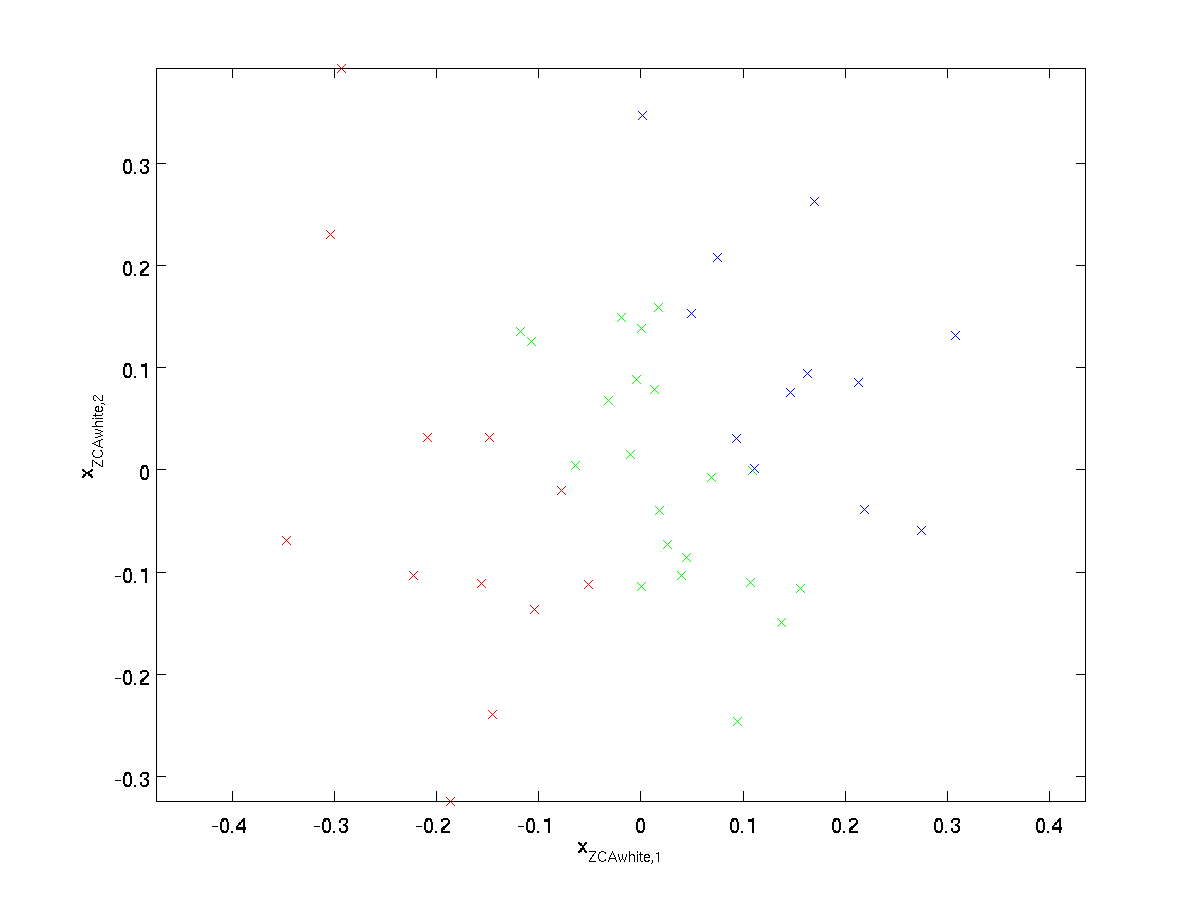
\includegraphics[width=0.8\textwidth]{figures/ZCA-whitened.png}
  %\caption{}\label{fig:zcawhiten}
\end{figure}

\cnt{It can be shown that out of all possible choices for $R$, this choice of rotation causes $x_{\rm ZCAwhite}$ to be as close as possible to the original input data $x$.}
    {可以证明,对所有可能的 $R$,这种旋转使得 $x_{\rm ZCAwhite}$ 尽可能地接近原始输入数据 $x$。}
    {}

\cnt{When using ZCA whitening (unlike PCA whitening), we usually keep all $n$ dimensions of the data, and do not try to reduce its dimension.}
    {当使用 ZCA白化时(不同于 PCA白化),我们通常保留数据的全部 $n$ 个维度,不尝试去降低它的维数。}
    {}

\subsubsection{\cnt{Regularizaton}{正则化}{}}

\cnt{When implementing PCA whitening or ZCA whitening in practice, sometimes some of the eigenvalues $\lambda_i$ will be numerically close to 0, and thus the scaling step where we divide by $\sqrt{\lambda_i}$ would involve dividing by a value close to zero; this may cause the data to blow up (take on large values) or otherwise be numerically unstable. In practice, we therefore implement this scaling step using a small amount of regularization, and add a small constant $\epsilon$ to the eigenvalues before taking their square root and inverse:}
    {实践中需要实现PCA白化或ZCA白化时,有时一些特征值 $\lambda_i$ 在数值上接近于0,这样在缩放步骤时我们除以 $\sqrt{\lambda_i}$ 将导致除以一个接近0的值;这可能使数据上溢 (赋为大数值)或造成数值不稳定。因而在实践中,我们使用少量的正则化实现这个缩放过程,即在取平方根和倒数之前给特征值加上一个很小的常数 $\epsilon$:}
    {}
\begin{align} x_{{\rm PCAwhite},i} = \frac{x_{{\rm rot},i} }{\sqrt{\lambda_i + \epsilon}}. \end{align}

\cnt{When $x$ takes values around $[-1,1]$, a value of $\epsilon \approx 10^{-5}$ might be typical.}
    {当 $x$ 在区间 $[-1,1]$ 上时, 一般取值为 $\epsilon \approx 10^{-5}$。}
    {}

\cnt{For the case of images, adding $\epsilon$ here also has the effect of slightly smoothing (or low-pass filtering) the input image. This also has a desirable effect of removing aliasing artifacts caused by the way pixels are laid out in an image, and can improve the features learned (details are beyond the scope of these notes).}
    {对图像来说, 这里加上 $\epsilon$,对输入图像也有一些平滑(或低通滤波)的作用。这样处理还能消除在图像的像素信息获取过程中产生的噪声,改善学习到的特征(细节超出了本文的范围)。}
    {}

\cnt{ZCA whitening is a form of pre-processing of the data that maps it from $x$ to $x_{\rm ZCAwhite}$. It turns out that this is also a rough model of how the biological eye (the retina) processes images. Specifically, as your eye perceives images, most adjacent ``pixels" in your eye will perceive very similar values, since adjacent parts of an image tend to be highly correlated in intensity. It is thus wasteful for your eye to have to transmit every pixel separately (via your optic nerve) to your brain. Instead, your retina performs a decorrelation operation (this is done via retinal neurons that compute a function called ``on center, off surround/off center, on surround") which is similar to that performed by ZCA. This results in a less redundant representation of the input image, which is then transmitted to your brain.}
    {ZCA 白化是一种数据预处理方法,它将数据从 $x$ 映射到 $x_{\rm ZCAwhite}$。 事实证明这也是一种生物眼睛(视网膜)处理图像的粗糙模型。具体而言,当你的眼睛感知图像时,由于一幅图像中相邻的部分在亮度上十分相关,大多数临近的“像素”在眼中被感知为相近的值。因此,如果人眼需要分别传输每个像素值(通过视觉神经)到大脑中,会非常不划算。取而代之的是,视网膜进行一个与ZCA中相似的去相关操作 (这是由视网膜上的ON-型和OFF-型光感受器细胞将光信号转变为神经信号完成的)。由此得到对输入图像的更低冗余的表示,并将它传输到大脑。}
    {}


\subsection{\cnt{Implementing PCA/Whitening}{实现主成分分析和白化}{}}

\cnt{In this section, we summarize the PCA, PCA whitening and ZCA whitening algorithms, and also describe how you can implement them using efficient linear algebra libraries.}
    {在这一节里,我们将总结PCA, PCA白化和ZCA白化算法,并描述如何使用高效的线性代数库来实现它们。}
    {}

\cnt{First, we need to ensure that the data has (approximately) zero-mean. For natural images, we achieve this (approximately) by subtracting the mean value of each image patch.}
    {首先,我们需要确保数据的均值(近似)为零。对于自然图像,我们通过减去每个图像块(patch)的均值(近似地)来达到这一目标。}
    {}

\cnt{We achieve this by computing the mean for each patch and subtracting it for each patch. In Matlab, we can do this by using}
    {为此,我们计算每个图像块的均值,并从每个图像块中减去它的均值。(译注:参见PCA一章中“对图像数据应用PCA算法”一节)。Matlab实现如下:}
    {}
\begin{lstlisting}[language=matlab]
avg = mean(x, 1);     % Compute the mean pixel intensity value separately for each patch. 
x = x - repmat(avg, size(x, 1), 1);
\end{lstlisting}

\cnt{Next, we need to compute $\Sigma = \frac{1}{m} \sum_{i=1}^m (x^{(i)})(x^{(i)})^T$. If you're implementing this in Matlab (or even if you're implementing this in C++, Java, etc., but have access to an efficient linear algebra library), doing it as an explicit sum is inefficient. Instead, we can compute this in one fell swoop as}
    {下面,我们要计算 $\Sigma = \frac{1}{m} \sum_{i=1}^m (x^{(i)})(x^{(i)})^T$,如果你在Matlab中实现(或者在C++, Java等中实现,但可以使用高效的线性代数库),直接求和效率很低。不过,我们可以这样一气呵成。}
    {}
\begin{lstlisting}[language=matlab]
sigma = x * x' / size(x, 2);
\end{lstlisting}

\cnt{(Check the math yourself for correctness.) Here, we assume that \texttt{x} is a data structure that contains one training example per column (so, \texttt{x} is a $n$-by-$m$ matrix).}
    {(自己推导一下看看)这里,我们假设 \texttt{x} 为一数据结构,其中每列表示一个训练样本(所以 \texttt{x} 是一个 $n \times m$ 的矩阵)。}
    {}

\cnt{Next, PCA computes the eigenvectors of $\Sigma$. One could do this using the Matlab \texttt{eig} function. However, because $\Sigma$ is a symmetric positive semi-definite matrix, it is more numerically reliable to do this using the svd function. Concretely, if you implement}
    {接下来,PCA计算 $\Sigma$ 的特征向量。你可以使用Matlab的 \texttt{eig} 函数来计算。但是由于 $\Sigma$ 是对称半正定的矩阵,用 svd 函数在数值计算上更加稳定。具体来说,如果你使用}
    {}
\begin{lstlisting}[language=matlab]
[U,S,V] = svd(sigma);
\end{lstlisting}
\cnt{then the matrix \texttt{U} will contain the eigenvectors of Sigma (one eigenvector per column, sorted in order from top to bottom eigenvector), and the diagonal entries of the matrix $S$ will contain the corresponding eigenvalues (also sorted in decreasing order). The matrix \texttt{V} will be equal to transpose of \texttt{U}, and can be safely ignored.}
    {那矩阵 \texttt{U} 将包含 Sigma 的特征向量(一个特征向量一列,从主向量开始排序),矩阵 \texttt{S} 对角线上的元素将包含对应的特征值(同样降序排列)。矩阵 \texttt{V} 等于 \texttt{U} 的转置,可以忽略。}
    {}

\cnt{(Note: The svd function actually computes the singular vectors and singular values of a matrix, which for the special case of a symmetric positive semi-definite matrix---which is all that we're concerned with here---is equal to its eigenvectors and eigenvalues. A full discussion of singular vectors vs. eigenvectors is beyond the scope of these notes.)}
    {(注意 svd 函数实际上计算的是一个矩阵的奇异值和奇异向量,就对称半正定矩阵的特殊情况来说,它们对应于特征值和特征向量,这里我们也只关心这一特例。关于奇异向量和特征向量的详细讨论超出了本文范围。)}
    {}

\cnt{Finally, you can compute $x_{\rm rot}$ and $\tilde{x}$ as follows:}
    {最后,我们可以这样计 算$x_{\rm rot}$ 和 $\tilde{x}$:}
    {}
\begin{lstlisting}[language=matlab]
xRot = U' * x;          % rotated version of the data. 
xTilde = U(:,1:k)' * x; % reduced dimension representation of the data, 
                        % where k is the number of eigenvectors to keep
\end{lstlisting}

\cnt{This gives your PCA representation of the data in terms of $\tilde{x} \in \Re^k$. Incidentally, if \texttt{x} is a $n$-by-$m$ matrix containing all your training data, this is a vectorized implementation, and the expressions above work too for computing $x_{\rm rot}$ and $\tilde{x}$ for your entire training set all in one go. The resulting $x_{\rm rot}$ and $\tilde{x}$ will have one column corresponding to each training example.}
    {这以 $\tilde{x} \in \Re^k$ 的形式给出了数据的PCA表示。顺便说一下,如果 \texttt{x} 是一个包括所有训练数据的 $n \times m$ 矩阵,这也是一种向量化的实现方式,上面的式子可以让你一次对所有的训练样本计算出 $x_{\rm rot}$ 和 $\tilde{x}$。得到的 $x_{\rm rot}$ 和 $\tilde{x}$ 中,每列对应一个训练样本。}
    {}

\cnt{To compute the PCA whitened data $x_{\rm PCAwhite}$, use}
    {为计算PCA白化后的数据 $x_{\rm PCAwhite}$,可以用}
    {}
\begin{lstlisting}[language=matlab]
xPCAwhite = diag(1./sqrt(diag(S) + epsilon)) * U' * x;
\end{lstlisting}

\cnt{Since $S$'s diagonal contains the eigenvalues $\lambda_i$, this turns out to be a compact way of computing $x_{{\rm PCAwhite},i} = \dfrac{x_{{\rm rot},i} }{\sqrt{\lambda_i}}$ simultaneously for all $i$.}
    {因为 $S$ 的对角线包括了特征值 $\lambda_i$,这其实就是同时为所有样本 $i$ 计算 $x_{{\rm PCAwhite},i} = \dfrac{x_{{\rm rot},i} }{\sqrt{\lambda_i}}$ 的简洁表达。}
    {}

\cnt{Finally, you can also compute the ZCA whitened data $x_{\rm ZCAwhite}$ as:}
    {最后,你也可以这样计算ZCA白化后的数据 $x_{\rm ZCAwhite}$:}
    {}
\begin{lstlisting}[language=matlab]
xZCAwhite = U * diag(1./sqrt(diag(S) + epsilon)) * U' * x;
\end{lstlisting}


\subsection{\cnt{Exercise:PCA in 2D}{练习:2D中的PCA}{}}

\cnt{PCA, PCA whitening and ZCA whitening in 2D}
    {}
    {}

\cnt{In this exercise you will implement PCA, PCA whitening and ZCA whitening, as described in the earlier sections of this tutorial, and generate the images shown in the earlier sections yourself. You will build on the starter code that has been provided at \url{http://ufldl.stanford.edu/wiki/resources/pca_2d.zip}. You need only write code at the places indicated by ``YOUR CODE HERE" in the files. The only file you need to modify is \texttt{pca\_2d.m}. Implementing this exercise will make the next exercise significantly easier to understand and complete.}
    {}
    {}


\subsubsection{\cnt{Step 0: Load data}{}{}}

\cnt{The starter code contains code to load 45 2D data points. When plotted using the scatter function, the results should look like the following:}
    {}
    {}

\begin{figure}[ht] \centering
  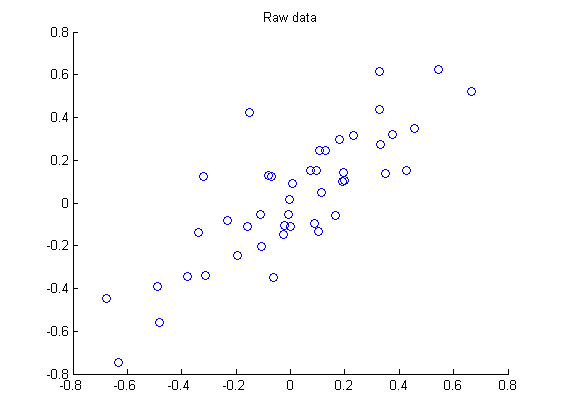
\includegraphics[width=0.8\textwidth]{figures/Raw_images_2d.png}
  %\caption{}\label{fig:zcawhiten}
\end{figure}

\subsubsection{\cnt{Step 1: Implement PCA}{}{}}

\cnt{In this step, you will implement PCA to obtain xrot, the matrix in which the data is ``rotated" to the basis comprising $u_1, \ldots, u_n$ made up of the principal components. As mentioned in the implementation notes, you should make use of MATLAB's svd function here.}
    {}
    {}

\subsubsection{\cnt{Step 1a: Finding the PCA basis}{}{}}

\cnt{Find $u_1$ and $u_2$, and draw two lines in your figure to show the resulting basis on top of the given data points. You may find it useful to use MATLAB's \texttt{hold on} and \texttt{hold off} functions. (After calling \texttt{hold on}, plotting functions such as \texttt{plot} will draw the new data on top of the previously existing figure rather than erasing and replacing it; and \texttt{hold off} turns this off.) You can use \texttt{plot([x1,x2], [y1,y2], '-')} to draw a line between \texttt{(x1,y1)} and \texttt{(x2,y2)}. Your figure should look like this:}
    {}
    {}

\begin{figure}[ht] \centering
  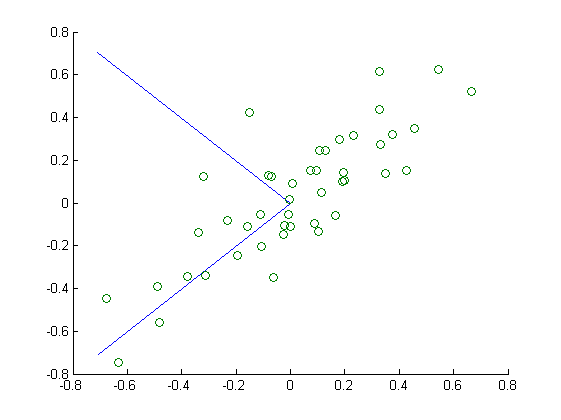
\includegraphics[width=0.8\textwidth]{figures/Pca_2d_basis.png}
  %\caption{}\label{fig:zcawhiten}
\end{figure}


\cnt{If you are doing this in Matlab, you will probably get a plot that's identical to ours. However, eigenvectors are defined only up to a sign. I.e., instead of returning $u_1$ as the first eigenvector, Matlab/Octave could just as easily have returned $-u_1$, and similarly instead of $u_2$ Matlab/Octave could have returned $-u_2$. So if you wound up with one or both of the eigenvectors pointing in a direction opposite (180 degrees difference) from what's shown above, that's okay too.}
    {}
    {}

\subsubsection{\cnt{Step 1b: Check xRot}{}{}}

\cnt{Compute \texttt{xRot}, and use the \texttt{scatter} function to check that \texttt{xRot} looks as it should, which should be something like the following:}
    {}
    {}

\begin{figure}[ht] \centering
  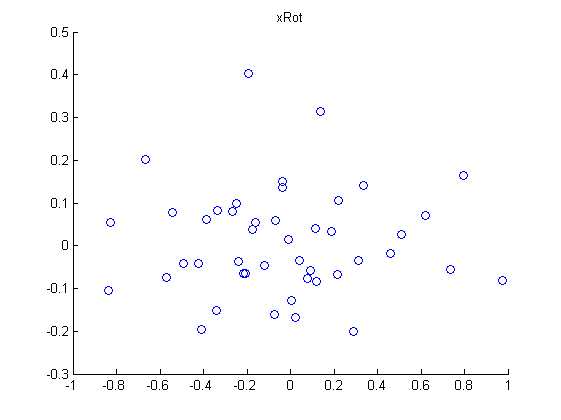
\includegraphics[width=0.8\textwidth]{figures/Pca_xrot_2d.png}
  %\caption{}\label{fig:zcawhiten}
\end{figure}


\cnt{Because Matlab/Octave could have returned $-u_1$ and/or $-u_2$ instead of $u_1$ and $u_2$, it's also possible that you might have gotten a figure which is ``flipped" or ``reflected" along the $x$- and/or $y$-axis; a flipped/reflected version of this figure is also a completely correct result.}
    {}
    {}

\subsubsection{\cnt{Step 2: Dimension reduce and replot}{}{}}

\cnt{In the next step, set $k$, the number of components to retain, to be 1 (we have already done this for you). Compute the resulting xHat and plot the results. You should get the following (this figure should not be flipped along the $x$- or $y$-axis):}
    {}
    {}

\begin{figure}[ht] \centering
  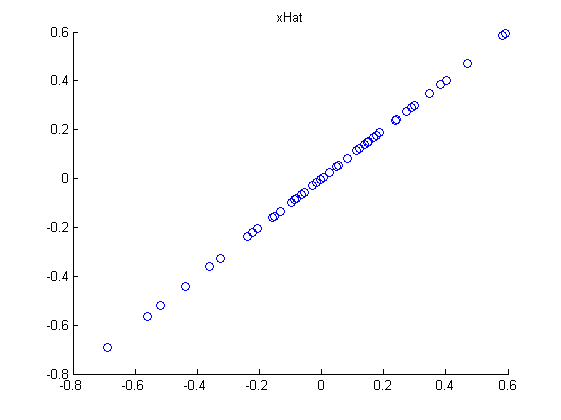
\includegraphics[width=0.8\textwidth]{figures/Pca_xhat_2d.png}
  %\caption{}\label{fig:zcawhiten}
\end{figure}


\subsubsection{\cnt{Step 3: PCA Whitening}{}{}}

\cnt{Implement PCA whitening using the formula from the notes. Plot \texttt{xPCAWhite}, and verify that it looks like the following (a figure that is flipped/reflected on either/both axes is also correct):}
    {}
    {}

\begin{figure}[ht] \centering
  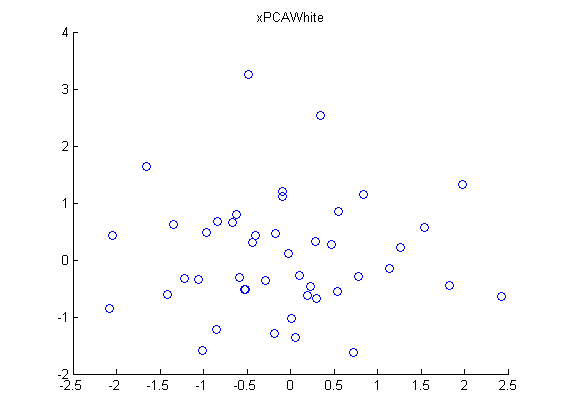
\includegraphics[width=0.8\textwidth]{figures/Pca_white_2d.png}
  %\caption{}\label{fig:zcawhiten}
\end{figure}

\subsubsection{\cnt{Step 4: ZCA Whitening}{}{}}

\cnt{Implement ZCA whitening and plot the results. The results should look like the following (this should not be flipped/reflected along the $x$- or $y$-axis):}
    {}
    {}

\begin{figure}[ht] \centering
  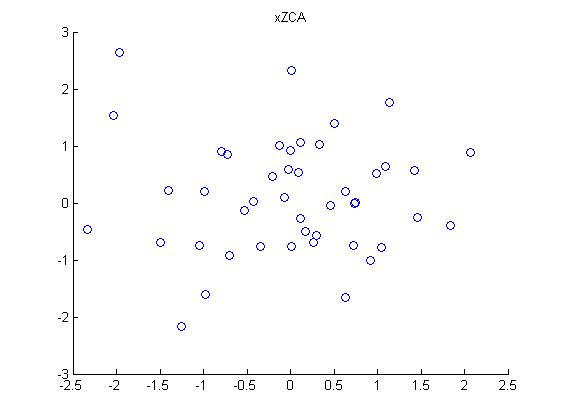
\includegraphics[width=0.8\textwidth]{figures/Zca_white_2d.png}
  %\caption{}\label{fig:zcawhiten}
\end{figure}





\subsection{\cnt{Exercise:PCA and Whitening}{练习:PCA和白化}{}}

\cnt{PCA and Whitening on natural images}
    {}
    {}


\cnt{In this exercise, you will implement PCA, PCA whitening and ZCA whitening, and apply them to image patches taken from natural images.}
    {}
    {}


\cnt{You will build on the MATLAB starter code which we have provided in \url{http://ufldl.stanford.edu/wiki/resources/pca_exercise.zip}{pca\_exercise.zip}. You need only write code at the places indicated by ``YOUR CODE HERE" in the files. The only file you need to modify is \texttt{pca\_gen.m}. }
    {}
    {}

\subsubsection{\cnt{Step 0: Prepare data}{}{}}

\textbf{\cnt{Step 0a: Load data}{}{}}

\cnt{The starter code contains code to load a set of natural images and sample $12 \times 12$ patches from them. The raw patches will look something like this:}
    {}
    {}

\begin{figure}[ht] \centering
  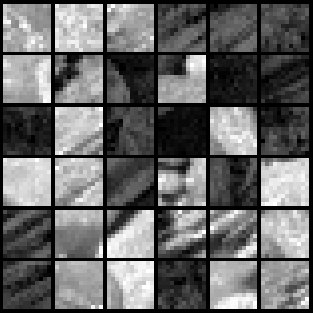
\includegraphics[width=0.5\textwidth]{figures/Raw_images.png}
  %\caption{}\label{fig:zcawhiten}
\end{figure}

\cnt{These patches are stored as column vectors $x^{(i)} \in \mathbb{R}^{144}$ in the $144 \times 10000$ matrix \texttt{x}.}
    {}
    {}

\textbf{\cnt{Step 0b: Zero mean the data}{}{}}

\cnt{First, for each image patch, compute the mean pixel value and subtract it from that image, this centering the image around zero. You should compute a different mean value for each image patch.}
    {}
    {}

\subsubsection{\cnt{Step 1: Implement PCA}{}{}}

\textbf{\cnt{Step 1a: Implement PCA}{}{}}

\cnt{n this step, you will implement PCA to obtain $x_{\rm rot}$, the matrix in which the data is ``rotated" to the basis comprising the principal components (i.e. the eigenvectors of $\Sigma$). Note that in this part of the exercise, you should not whiten the data.}
    {}
    {}

\textbf{\cnt{Step 1b: Check covariance}{}{}}

\cnt{To verify that your implementation of PCA is correct, you should check the covariance matrix for the rotated data $x_{\rm rot}$. PCA guarantees that the covariance matrix for the rotated data is a diagonal matrix (a matrix with non-zero entries only along the main diagonal). Implement code to compute the covariance matrix and verify this property. One way to do this is to compute the covariance matrix, and visualise it using the MATLAB command imagesc. The image should show a coloured diagonal line against a blue background. For this dataset, because of the range of the diagonal entries, the diagonal line may not be apparent, so you might get a figure like the one show below, but this trick of visualizing using imagesc will come in handy later in this exercise.}
    {}
    {}

\begin{figure}[ht] \centering
  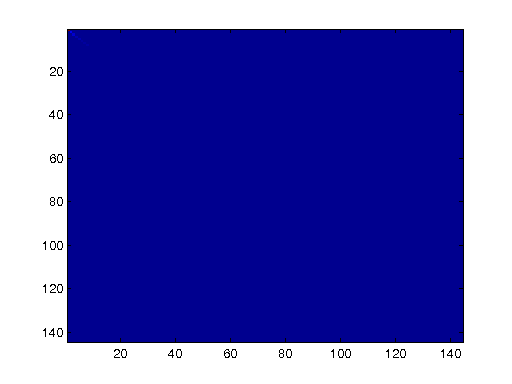
\includegraphics[width=0.4\textwidth]{figures/Pca_covar.png}
  %\caption{}\label{fig:zcawhiten}
\end{figure}

\subsubsection{\cnt{Step 2: Find number of components to retain}{}{}}

\cnt{Next, choose k, the number of principal components to retain. Pick $k$ to be as small as possible, but so that at least 99\% of the variance is retained. In the step after this, you will discard all but the top $k$ principal components, reducing the dimension of the original data to k.}
    {}
    {}

\subsubsection{\cnt{Step 3: PCA with dimension reduction}{}{}}

\cnt{Now that you have found $k$, compute $\tilde{x}$, the reduced-dimension representation of the data. This gives you a representation of each image patch as a $k$ dimensional vector instead of a 144 dimensional vector. If you are training a sparse autoencoder or other algorithm on this reduced-dimensional data, it will run faster than if you were training on the original 144 dimensional data.}
    {}
    {}

\cnt{To see the effect of dimension reduction, go back from $\tilde{x}$ to produce the matrix $\hat{x}$, the dimension-reduced data but expressed in the original 144 dimensional space of image patches. Visualise $\hat{x}$ and compare it to the raw data, $x$. You will observe that there is little loss due to throwing away the principal components that correspond to dimensions with low variation. For comparison, you may also wish to generate and visualise $\hat{x}$ for when only 90\% of the variance is retained.}
    {}
    {}

\begin{figure}[ht] \centering
  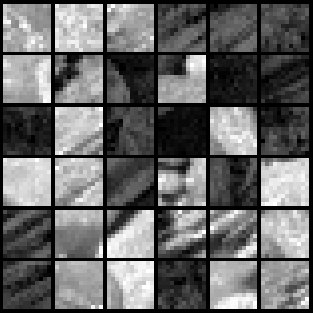
\includegraphics[width=0.3\textwidth]{figures/Raw_images.png} \caption{Raw images}
  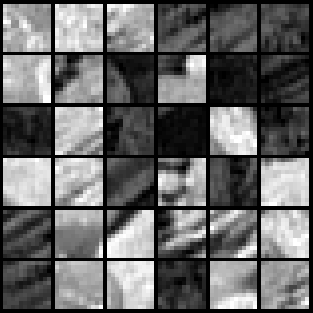
\includegraphics[width=0.3\textwidth]{figures/Pca_images.png} \caption{PCA dimension-reduced images (99\% variance)}
  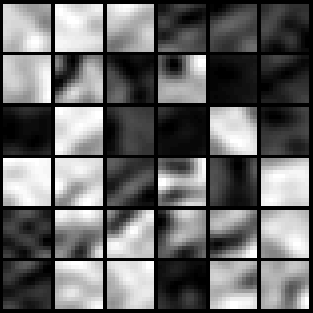
\includegraphics[width=0.3\textwidth]{figures/Pca_images_90.png} \caption{PCA dimension-reduced images (90\% variance)}
  %\caption{}\label{fig:zcawhiten}
\end{figure}

\subsubsection{\cnt{Step 4: PCA with whitening and regularization}{}{}}

\textbf{\cnt{Step 4a: Implement PCA with whitening and regularization}{}{}}

\cnt{Now implement PCA with whitening and regularization to produce the matrix \texttt{xPCAWhite}. Use the following parameter value:}
    {}
    {}
\begin{lstlisting}[language=matlab]
epsilon = 0.1
\end{lstlisting}

\textbf{\cnt{Step 4b: Check covariance}{}{}}

\cnt{Similar to using PCA alone, PCA with whitening also results in processed data that has a diagonal covariance matrix. However, unlike PCA alone, whitening additionally ensures that the diagonal entries are equal to 1, i.e. that the covariance matrix is the identity matrix.}
    {}
    {}

\cnt{That would be the case if you were doing whitening alone with no regularization. However, in this case you are whitening with regularization, to avoid numerical/etc. problems associated with small eigenvalues. As a result of this, some of the diagonal entries of the covariance of your \texttt{xPCAwhite} will be smaller than 1.}
    {}
    {}

\cnt{To verify that your implementation of PCA whitening with and without regularization is correct, you can check these properties. Implement code to compute the covariance matrix and verify this property. (To check the result of PCA without whitening, simply set epsilon to 0, or close to 0, say 1e-10). As earlier, you can visualise the covariance matrix with imagesc. When visualised as an image, for PCA whitening without regularization you should see a red line across the diagonal (corresponding to the one entries) against a blue background (corresponding to the zero entries); for PCA whitening with regularization you should see a red line that slowly turns blue across the diagonal (corresponding to the 1 entries slowly becoming smaller).}
    {}
    {}

\begin{figure}[ht] \centering
  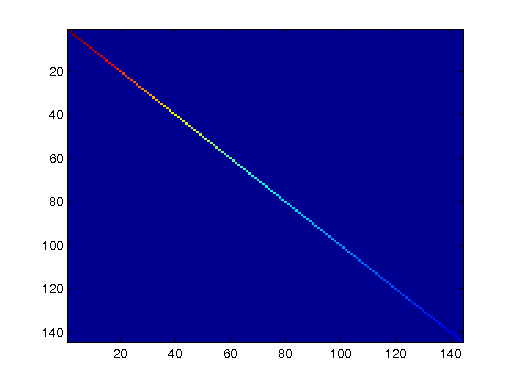
\includegraphics[width=0.4\textwidth]{figures/Pca_whitened_covar.png} \caption{Covariance for PCA whitening with regularization}
  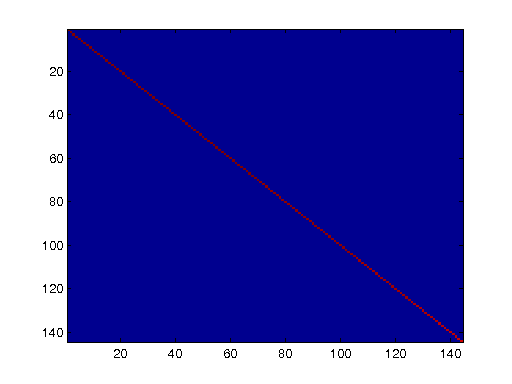
\includegraphics[width=0.4\textwidth]{figures/Pca_whitened_unregularised_covar.png} \caption{Covariance for PCA whitening without regularization}
  %\caption{}\label{fig:zcawhiten}
\end{figure}

\subsubsection{\cnt{Step 5: ZCA whitening}{}{}}

\cnt{Now implement ZCA whitening to produce the matrix \texttt{xZCAWhite}. Visualize \texttt{xZCAWhite} and compare it to the raw data, $x$. You should observe that whitening results in, among other things, enhanced edges. Try repeating this with epsilon set to 1, 0.1, and 0.01, and see what you obtain. The example shown below (left image) was obtained with epsilon = 0.1.}
    {}
    {}

\begin{figure}[ht] \centering
  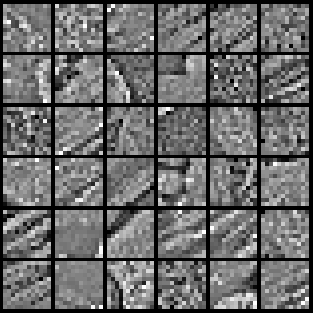
\includegraphics[width=0.4\textwidth]{figures/Zca_whitened_images.png} \caption{ZCA whitened images}
  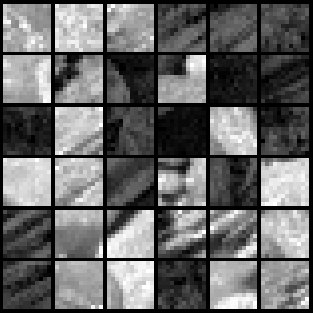
\includegraphics[width=0.4\textwidth]{figures/Raw_images.png} \caption{Raw images}
  %\caption{}\label{fig:zcawhiten}
\end{figure}




\clearpage
%# -*- coding: utf-8 -*-
%!TEX encoding = UTF-8 Unicode
%!TEX TS-program = xelatex
% vim:ts=4:sw=4
%
% 以上设定默认使用 XeLaTex 编译,并指定 Unicode 编码,供 TeXShop 自动识别

% Author: Yunhui Fu <yhfudev@gmail.com>
% License: Creative Commons (CC BY 4.0)

\section{\cnt{Softmax Regression}{Softmax回归}{}} \label{chp:softmaxreg}

\subsection{\cnt{Softmax Regression}{Softmax回归}{}}

\subsubsection{\cnt{Introduction}{介绍}{}}

\cnt{In these notes, we describe the \emph{Softmax regression} model. This model generalizes logistic regression to classification problems where the class label $y$ can take on more than two possible values. This will be useful for such problems as MNIST digit classification, where the goal is to distinguish between 10 different numerical digits. Softmax regression is a supervised learning algorithm, but we will later be using it in conjuction with our deep learning/unsupervised feature learning methods.}
    {在本节中,我们介绍 \emph{Softmax回归}模型,该模型是logistic回归模型在多分类问题上的推广,在多分类问题中,类标签 $y$ 可以取两个以上的值。 Softmax回归模型对于诸如 MNIST\footnote{译者注: MNIST 是一个手写数字识别库,由NYU 的Yann LeCun 等人维护。\url{http://yann.lecun.com/exdb/mnist/}.} 手写数字分类等问题是很有用的,该问题的目的是辨识10个不同的单个数字。Softmax回归是有监督的,不过后面也会介绍它与深度学习/无监督学习方法的结合。}
    {}


\cnt{Recall that in logistic regression, we had a training set $\{ (x^{(1)}, y^{(1)}), \ldots, (x^{(m)}, y^{(m)}) \}$ of $m$ labeled examples, where the input features are $x^{(i)} \in \Re^{n+1}$. (In this set of notes, we will use the notational convention of letting the feature vectors $x$ be $n + 1$ dimensional, with $x_0 = 1$ corresponding to the intercept term.) With logistic regression, we were in the binary classification setting, so the labels were $y^{(i)} \in \{0,1\}$. Our hypothesis took the form:}
    {回想一下在 logistic 回归中,我们的训练集由 $m$ 个已标记的样本构成:$\{ (x^{(1)}, y^{(1)}), \ldots, (x^{(m)}, y^{(m)}) \}$,其中输入特征 $x^{(i)} \in \Re^{n+1}$。(我们对符号的约定如下:特征向量 $x$ 的维度为 $n+1$,其中 $x_0 = 1$ 对应截距项 。) 由于 logistic 回归是针对二分类问题的,因此类标记 $y^{(i)} \in \{0,1\}$。假设函数(hypothesis function) 如下:}
    {}
\begin{align} h_\theta(x) = \frac{1}{1+\exp(-\theta^Tx)}, \end{align}

\cnt{and the model parameters $\theta$ were trained to minimize the cost function}
    {我们将训练模型参数 $\theta$,使其能够最小化代价函数 :}
    {}
\begin{align} J(\theta) = -\frac{1}{m} \left[ \sum_{i=1}^m y^{(i)} \log h_\theta(x^{(i)}) + (1-y^{(i)}) \log (1-h_\theta(x^{(i)})) \right] \end{align}

\cnt{In the softmax regression setting, we are interested in multi-class classification (as opposed to only binary classification), and so the label y can take on k different values, rather than only two. Thus, in our training set $\{ (x^{(1)}, y^{(1)}), \ldots, (x^{(m)}, y^{(m)}) \}$, we now have that $y^{(i)} \in \{1, 2, \ldots, k\}$. (Note that our convention will be to index the classes starting from 1, rather than from 0.) For example, in the MNIST digit recognition task, we would have $k = 10$ different classes.}
    {在 softmax回归中,我们解决的是多分类问题(相对于 logistic 回归解决的二分类问题),类标 $y$ 可以取 $k$ 个不同的值(而不是 2 个)。因此,对于训练集 $\{ (x^{(1)}, y^{(1)}), \ldots, (x^{(m)}, y^{(m)}) \}$,我们有 $y^{(i)} \in \{1, 2, \ldots, k\}$。(注意此处的类别下标从 1 开始,而不是 0)。例如,在 MNIST 数字识别任务中,我们有 $k=10$ 个不同的类别。}
    {}


\cnt{Given a test input $x$, we want our hypothesis to estimate the probability that $p(y = j | x)$ for each value of $j = 1, \ldots, k$. I.e., we want to estimate the probability of the class label taking on each of the $k$ different possible values. Thus, our hypothesis will output a $k$ dimensional vector (whose elements sum to 1) giving us our $k$ estimated probabilities. Concretely, our hypothesis $h_{\theta}(x)$ takes the form:}
    {对于给定的测试输入 $x$,我们想用假设函数针对每一个类别j估算出概率值 $p(y=j | x)$。也就是说,我们想估计 $x$ 的每一种分类结果出现的概率。因此,我们的假设函数将要输出一个 $k$ 维的向量(向量元素的和为1)来表示这 $k$ 个估计的概率值。 具体地说,我们的假设函数 $h_{\theta}(x)$ 形式如下:}
    {}
\begin{align} h_\theta(x^{(i)}) = \begin{bmatrix} p(y^{(i)} = 1 | x^{(i)}; \theta) \\ p(y^{(i)} = 2 | x^{(i)}; \theta) \\ \vdots \\ p(y^{(i)} = k | x^{(i)}; \theta) \end{bmatrix} = \frac{1}{ \sum_{j=1}^{k}{e^{ \theta_j^T x^{(i)}}}} \begin{bmatrix} e^{ \theta_1^T x^{(i)}} \\ e^{ \theta_2^T x^{(i)}} \\ \vdots \\ e^{ \theta_k^T x^{(i)}} \\ \end{bmatrix} \end{align}


\cnt{Here $\theta_1, \theta_2, \ldots, \theta_k \in \Re^{n+1}$ are the parameters of our model. Notice that the term $\frac{1}{ \sum_{j=1}^{k}{e^{ \theta_j^T x^{(i)}}}}$ normalizes the distribution, so that it sums to one.}
    {其中 $\theta_1, \theta_2, \ldots, \theta_k \in \Re^{n+1}$ 是模型的参数。请注意 $\frac{1}{ \sum_{j=1}^{k}{e^{ \theta_j^T x^{(i)}}}}$ 这一项对概率分布进行归一化,使得所有概率之和为 1 。}
    {}

\cnt{For convenience, we will also write $\theta$ to denote all the parameters of our model. When you implement softmax regression, it is usually convenient to represent $\theta$ as a $k$-by-$(n + 1)$ matrix obtained by stacking up $\theta_1, \theta_2, \ldots, \theta_k$ in rows, so that}
    {为了方便起见,我们同样使用符号 $\theta$ 来表示全部的模型参数。在实现Softmax回归时,将 $\theta$ 用一个 $k \times (n+1)$ 的矩阵来表示会很方便,该矩阵是将 $\theta_1, \theta_2, \ldots, \theta_k$ 按行罗列起来得到的,如下所示:}
    {}
$$
\theta = \begin{bmatrix} \mbox{---} \theta_1^T \mbox{---} \\ \mbox{---} \theta_2^T \mbox{---} \\ \vdots \\ \mbox{---} \theta_k^T \mbox{---} \\ \end{bmatrix}
$$

\subsubsection{\cnt{Cost Function}{代价函数}{}}

\cnt{We now describe the cost function that we'll use for softmax regression. In the equation below, $1\{\cdot\}$ is the indicator function, so that $1\{{\rm \texttt{a true statement}}\} = 1$, and $1\{{\rm \texttt{a false statement}}\} = 0$. For example, $1\{2 + 2 = 4\}$ evaluates to 1; whereas $1\{1 + 1 = 5\}$ evaluates to 0. Our cost function will be:}
    {现在我们来介绍 softmax 回归算法的代价函数。在下面的公式中,$1\{\cdot\}$ 是示性函数,其取值规则为:$1\{ {\rm \texttt{值为真的表达式}} \}=1$, $1\{ {\rm \texttt{值为假的表达式}} \}=0$。举例来说,表达式 $1\{2+2=4\}$ 的值为1 ,$1\{1+1=5\}$的值为 0。我们的代价函数为:}
    {}

\begin{align} J(\theta) = - \frac{1}{m} \left[ \sum_{i=1}^{m} \sum_{j=1}^{k} 1\left\{y^{(i)} = j\right\} \log \frac{e^{\theta_j^T x^{(i)}}}{\sum_{l=1}^k e^{ \theta_l^T x^{(i)}}}\right] \end{align}

\cnt{Notice that this generalizes the logistic regression cost function, which could also have been written:}
    {值得注意的是,上述公式是logistic回归代价函数的推广。logistic回归代价函数可以改为:}
    {}

\begin{align} J(\theta) &= -\frac{1}{m} \left[ \sum_{i=1}^m (1-y^{(i)}) \log (1-h_\theta(x^{(i)})) + y^{(i)} \log h_\theta(x^{(i)}) \right] \\ &= - \frac{1}{m} \left[ \sum_{i=1}^{m} \sum_{j=0}^{1} 1\left\{y^{(i)} = j\right\} \log p(y^{(i)} = j | x^{(i)} ; \theta) \right] \end{align}

\cnt{The softmax cost function is similar, except that we now sum over the $k$ different possible values of the class label. Note also that in softmax regression, we have that}
    {可以看到,Softmax代价函数与logistic 代价函数在形式上非常类似,只是在Softmax损失函数中对类标记的 $k$ 个可能值进行了累加。注意在Softmax回归中将 $x$ 分类为类别 $j$ 的概率为:}
    {}
$p(y^{(i)} = j | x^{(i)} ; \theta) = \frac{e^{\theta_j^T x^{(i)}}}{\sum_{l=1}^k e^{ \theta_l^T x^{(i)}}}$ .

\cnt{There is no known closed-form way to solve for the minimum of $J(\theta)$, and thus as usual we'll resort to an iterative optimization algorithm such as gradient descent or L-BFGS. Taking derivatives, one can show that the gradient is:}
    {对于 $J(\theta)$ 的最小化问题,目前还没有闭式解法。因此,我们使用迭代的优化算法(例如梯度下降法,或 L-BFGS)。经过求导,我们得到梯度公式如下:}
    {}
\begin{align} \nabla_{\theta_j} J(\theta) = - \frac{1}{m} \sum_{i=1}^{m}{ \left[ x^{(i)} \left( 1\{ y^{(i)} = j\} - p(y^{(i)} = j | x^{(i)}; \theta) \right) \right]} \end{align}


\cnt{Recall the meaning of the ``$\nabla_{\theta_j}$" notation. In particular, $\nabla_{\theta_j} J(\theta)$ is itself a vector, so that its $l$-th element is $\frac{\partial J(\theta)}{\partial \theta_{jl}}$ the partial derivative of $J(\theta)$ with respect to the $l$-th element of $\theta_j$.}
    {让我们来回顾一下符号 ``$\nabla_{\theta_j}$" 的含义。$\nabla_{\theta_j} J(\theta)$ 本身是一个向量,它的第 $l$ 个元素 $\frac{\partial J(\theta)}{\partial \theta_{jl}}$ 是 $J(\theta)$ 对 $\theta_j$ 的第 $l$ 个分量的偏导数。}
    {}


\cnt{Armed with this formula for the derivative, one can then plug it into an algorithm such as gradient descent, and have it minimize $J(\theta)$. For example, with the standard implementation of gradient descent, on each iteration we would perform the update $\theta_j := \theta_j - \alpha \nabla_{\theta_j} J(\theta)$ (for each $j=1,\ldots,k$).}
    {有了上面的偏导数公式以后,我们就可以将它代入到梯度下降法等算法中,来最小化 $J(\theta)$。 例如,在梯度下降法的标准实现中,每一次迭代需要进行如下更新: $\theta_j := \theta_j - \alpha \nabla_{\theta_j} J(\theta)$ ( $j=1,\ldots,k$)。}
    {}


\cnt{When implementing softmax regression, we will typically use a modified version of the cost function described above; specifically, one that incorporates weight decay. We describe the motivation and details below.}
    {当实现 softmax 回归算法时, 我们通常会使用上述代价函数的一个改进版本。具体来说,就是和权重衰减(weight decay)一起使用。我们接下来介绍使用它的动机和细节。}
    {}


\subsubsection{\cnt{Properties of softmax regression parameterization}{Softmax回归模型参数化的特点}{}}

\cnt{Softmax regression has an unusual property that it has a ``redundant" set of parameters. To explain what this means, suppose we take each of our parameter vectors $\theta_j$, and subtract some fixed vector $\psi$ from it, so that every $\theta_j$ is now replaced with $\theta_j - \psi$ (for every $j=1, \ldots, k$). Our hypothesis now estimates the class label probabilities as}
    {Softmax 回归有一个不寻常的特点:它有一个“冗余”的参数集。为了便于阐述这一特点,假设我们从参数向量 $\theta_j$ 中减去了向量 $\psi$,这时,每一个 $\theta_j$ 都变成了 $\theta_j - \psi$ ($j=1, \ldots, k$)。此时假设函数变成了以下的式子:}
    {}
\begin{align} p(y^{(i)} = j | x^{(i)} ; \theta) &= \frac{e^{(\theta_j-\psi)^T x^{(i)}}}{\sum_{l=1}^k e^{ (\theta_l-\psi)^T x^{(i)}}} \\ &= \frac{e^{\theta_j^T x^{(i)}} e^{-\psi^Tx^{(i)}}}{\sum_{l=1}^k e^{\theta_l^T x^{(i)}} e^{-\psi^Tx^{(i)}}} \\ &= \frac{e^{\theta_j^T x^{(i)}}}{\sum_{l=1}^k e^{ \theta_l^T x^{(i)}}}. \end{align}

\cnt{In other words, subtracting $\psi$ from every $\theta_j$ does not affect our hypothesis' predictions at all! This shows that softmax regression's parameters are ``redundant." More formally, we say that our softmax model is overparameterized, meaning that for any hypothesis we might fit to the data, there are multiple parameter settings that give rise to exactly the same hypothesis function $h_\theta$ mapping from inputs $x$ to the predictions.}
    {换句话说,从 $\theta_j$ 中减去 $\psi$ 完全不影响假设函数的预测结果!这表明前面的 softmax 回归模型中存在冗余的参数。更正式一点来说, Softmax 模型被过度参数化了。对于任意一个用于拟合数据的假设函数,可以求出多组参数值,这些参数得到的是完全相同的假设函数 $h_\theta$。}
    {}


\cnt{Further, if the cost function $J(\theta)$ is minimized by some setting of the parameters $(\theta_1, \theta_2,\ldots, \theta_k)$, then it is also minimized by $(\theta_1 - \psi, \theta_2 - \psi,\ldots, \theta_k - \psi)$ for any value of $\psi$. Thus, the minimizer of $J(\theta)$ is not unique. (Interestingly, $J(\theta)$ is still convex, and thus gradient descent will not run into a local optima problems. But the Hessian is singular/non-invertible, which causes a straightforward implementation of Newton's method to run into numerical problems.)}
    {进一步而言,如果参数 $(\theta_1, \theta_2,\ldots, \theta_k)$ 是代价函数 $J(\theta)$ 的极小值点,那么 $(\theta_1 - \psi, \theta_2 - \psi,\ldots, \theta_k - \psi)$ 同样也是它的极小值点,其中 $\psi$ 可以为任意向量。因此使 $J(\theta)$ 最小化的解不是唯一的。(有趣的是,由于 $J(\theta)$ 仍然是一个凸函数,因此梯度下降时不会遇到局部最优解的问题。但是 Hessian 矩阵是奇异的/不可逆的,这会直接导致采用牛顿法优化就遇到数值计算的问题)}
    {}


\cnt{Notice also that by setting $\psi = \theta_1$, one can always replace $\theta_1$ with $\theta_1 - \psi = \vec{0}$ (the vector of all 0's), without affecting the hypothesis. Thus, one could ``eliminate" the vector of parameters $\theta_1$ (or any other $\theta_j$, for any single value of $j$), without harming the representational power of our hypothesis. Indeed, rather than optimizing over the $k(n + 1)$ parameters $(\theta_1, \theta_2,\ldots, \theta_k)$ (where $\theta_j \in \Re^{n+1}$), one could instead set $\theta_1 = \vec{0}$ and optimize only with respect to the $(k − 1)(n + 1)$ remaining parameters, and this would work fine.}
    {注意,当 $\psi = \theta_1$ 时,我们总是可以将 $\theta_1$ 替换为 $\theta_1 - \psi = \vec{0}$(即替换为全零向量),并且这种变换不会影响假设函数。因此我们可以去掉参数向量 $\theta_1$ (或者其他 $\theta_j$ 中的任意一个)而不影响假设函数的表达能力。实际上,与其优化全部的 $k\times(n+1)$ 个参数 $(\theta_1, \theta_2,\ldots, \theta_k)$ (其中 $\theta_j \in \Re^{n+1}$),我们可以令 $\theta_1 = \vec{0}$,只优化剩余的 $(k-1)\times(n+1)$ 个参数,这样算法依然能够正常工作。}
    {}


\cnt{In practice, however, it is often cleaner and simpler to implement the version which keeps all the parameters $(\theta_1, \theta_2,\ldots, \theta_n)$, without arbitrarily setting one of them to zero. But we will make one change to the cost function: Adding weight decay. This will take care of the numerical problems associated with softmax regression's overparameterized representation.}
    {在实际应用中,为了使算法实现更简单清楚,往往保留所有参数 $(\theta_1, \theta_2,\ldots, \theta_n)$,而不任意地将某一参数设置为 0。但此时我们需要对代价函数做一个改动:加入权重衰减。权重衰减可以解决 softmax 回归的参数冗余所带来的数值问题。}
    {}


\subsubsection{\cnt{Weight Decay}{权重衰减}{}}

\cnt{We will modify the cost function by adding a weight decay term $\frac{\lambda}{2} \sum_{i=1}^k \sum_{j=0}^{n} \theta_{ij}^2$ which penalizes large values of the parameters. Our cost function is now}
    {我们通过添加一个权重衰减项 $\frac{\lambda}{2} \sum_{i=1}^k \sum_{j=0}^{n} \theta_{ij}^2$ 来修改代价函数,这个衰减项会惩罚过大的参数值,现在我们的代价函数变为:}
    {}
\begin{align} J(\theta) = - \frac{1}{m} \left[ \sum_{i=1}^{m} \sum_{j=1}^{k} 1\left\{y^{(i)} = j\right\} \log \frac{e^{\theta_j^T x^{(i)}}}{\sum_{l=1}^k e^{ \theta_l^T x^{(i)}}} \right] + \frac{\lambda}{2} \sum_{i=1}^k \sum_{j=0}^n \theta_{ij}^2 \end{align}

\cnt{With this weight decay term (for any $\lambda > 0$), the cost function $J(\theta)$ is now strictly convex, and is guaranteed to have a unique solution. The Hessian is now invertible, and because $J(\theta)$ is convex, algorithms such as gradient descent, L-BFGS, etc. are guaranteed to converge to the global minimum.}
    {有了这个权重衰减项以后 ($\lambda > 0$),代价函数就变成了严格的凸函数,这样就可以保证得到唯一的解了。 此时的 Hessian矩阵变为可逆矩阵,并且因为$J(\theta)$是凸函数,梯度下降法和 L-BFGS 等算法可以保证收敛到全局最优解。}
    {}


\cnt{To apply an optimization algorithm, we also need the derivative of this new definition of $J(\theta)$. One can show that the derivative is:}
    {为了使用优化算法,我们需要求得这个新函数 $J(\theta)$ 的导数,如下:}
    {}
\begin{align} \nabla_{\theta_j} J(\theta) = - \frac{1}{m} \sum_{i=1}^{m}{ \left[ x^{(i)} ( 1\{ y^{(i)} = j\} - p(y^{(i)} = j | x^{(i)}; \theta) ) \right]} + \lambda \theta_j \end{align}

\cnt{By minimizing $J(\theta)$ with respect to $\theta$, we will have a working implementation of softmax regression.}
    {通过最小化 $J(\theta)$,我们就能实现一个可用的 softmax 回归模型。}
    {}

\subsubsection{\cnt{Relationship to Logistic Regression}{Softmax回归与Logistic 回归的关系}{}}

\cnt{In the special case where $k = 2$, one can show that softmax regression reduces to logistic regression. This shows that softmax regression is a generalization of logistic regression. Concretely, when $k = 2$, the softmax regression hypothesis outputs}
    {当类别数 $k = 2$ 时,softmax 回归退化为 logistic 回归。这表明 softmax 回归是 logistic 回归的一般形式。具体地说,当 $k = 2$ 时,softmax 回归的假设函数为:}
    {}
\begin{align} h_\theta(x) &= \frac{1}{ e^{\theta_1^Tx} + e^{ \theta_2^T x^{(i)}}} \begin{bmatrix} e^{ \theta_1^T x} \\ e^{ \theta_2^T x} \end{bmatrix} \end{align}

\cnt{Taking advantage of the fact that this hypothesis is overparameterized and setting $\psi = \theta_1$, we can subtract $\theta_1$ from each of the two parameters, giving us}
    {利用softmax回归参数冗余的特点,我们令 $\psi = \theta_1$,并且从两个参数向量中都减去向量 $\theta_1$,得到:}
    {}


\begin{align} h(x) &= \frac{1}{ e^{\vec{0}^Tx} + e^{ (\theta_2-\theta_1)^T x^{(i)}}} \begin{bmatrix} e^{ \vec{0}^T x} \\ e^{ (\theta_2-\theta_1)^T x} \end{bmatrix} \\ &= \begin{bmatrix} \frac{1}{ 1 + e^{ (\theta_2-\theta_1)^T x^{(i)}}} \\ \frac{e^{ (\theta_2-\theta_1)^T x}}{ 1 + e^{ (\theta_2-\theta_1)^T x^{(i)}}} \end{bmatrix} \\ &= \begin{bmatrix} \frac{1}{ 1 + e^{ (\theta_2-\theta_1)^T x^{(i)}}} \\ 1 - \frac{1}{ 1 + e^{ (\theta_2-\theta_1)^T x^{(i)}}} \\ \end{bmatrix} \end{align}


\cnt{Thus, replacing $\theta_2 − \theta_1$ with a single parameter vector $\theta'$, we find that softmax regression predicts the probability of one of the classes as $\frac{1}{ 1 + e^{ (\theta')^T x^{(i)}}}$, and that of the other class as $1 - \frac{1}{ 1 + e^{ (\theta')^T x^{(i)}}}$, same as logistic regression.}
    {因此,用 $\theta'$ 来表示 $\theta_2-\theta_1$,我们就会发现 softmax 回归器预测其中一个类别的概率为 $\frac{1}{ 1 + e^{ (\theta')^T x^{(i)}}}$,另一个类别概率的为 $1 - \frac{1}{ 1 + e^{ (\theta')^T x^{(i)}}}$,这与 logistic回归是一致的。}
    {}


\subsubsection{\cnt{Softmax Regression vs. $k$ Binary Classifiers}{Softmax 回归 vs. $k$ 个二元分类器}{}}

\cnt{Suppose you are working on a music classification application, and there are $k$ types of music that you are trying to recognize. Should you use a softmax classifier, or should you build $k$ separate binary classifiers using logistic regression?}
    {如果你在开发一个音乐分类的应用,需要对$k$种类型的音乐进行识别,那么是选择使用 softmax 分类器呢,还是使用 logistic 回归算法建立 $k$ 个独立的二元分类器呢?}
    {}


\cnt{This will depend on whether the four classes are mutually exclusive. For example, if your four classes are classical, country, rock, and jazz, then assuming each of your training examples is labeled with exactly one of these four class labels, you should build a softmax classifier with $k = 4$. (If there're also some examples that are none of the above four classes, then you can set $k = 5$ in softmax regression, and also have a fifth, ``none of the above," class.)}
    {这一选择取决于你的类别之间是否互斥,例如,如果你有四个类别的音乐,分别为:古典音乐、乡村音乐、摇滚乐和爵士乐,那么你可以假设每个训练样本只会被打上一个标签(即:一首歌只能属于这四种音乐类型的其中一种),此时你应该使用类别数 $k = 4$ 的softmax回归。(如果在你的数据集中,有的歌曲不属于以上四类的其中任何一类,那么你可以添加一个“其他类”,并将类别数 $k$ 设为5。)}
    {}


\cnt{If however your categories are \texttt{has\_vocals}, dance, soundtrack, pop, then the classes are not \emph{mutually exclusive}; for example, there can be a piece of pop music that comes from a soundtrack and in addition has vocals. In this case, it would be more appropriate to build 4 binary logistic regression classifiers. This way, for each new musical piece, your algorithm can separately decide whether it falls into each of the four categories.}
    {如果你的四个类别如下:人声音乐、舞曲、影视原声、流行歌曲,那么这些类别之间并不是互斥的。例如:一首歌曲可以来源于影视原声,同时也包含人声 。这种情况下,使用4个二分类的 logistic 回归分类器更为合适。这样,对于每个新的音乐作品 ,我们的算法可以分别判断它是否属于各个类别。}
    {}


\cnt{Now, consider a computer vision example, where you're trying to classify images into three different classes. (i) Suppose that your classes are \texttt{indoor\_scene, outdoor\_urban\_scene}, and \texttt{outdoor\_wilderness\_scene}. Would you use sofmax regression or three logistic regression classifiers? (ii) Now suppose your classes are indoor\_scene, black\_and\_white\_image, and image\_has\_people. Would you use softmax regression or multiple logistic regression classifiers?}
    {现在我们来看一个计算视觉领域的例子,你的任务是将图像分到三个不同类别中。(i) 假设这三个类别分别是:室内场景、户外城区场景、户外荒野场景。你会使用sofmax回归还是 3个logistic 回归分类器呢? (ii) 现在假设这三个类别分别是室内场景、黑白图片、包含人物的图片,你又会选择 softmax 回归还是多个 logistic 回归分类器呢?}
    {}


\cnt{In the first case, the classes are mutually exclusive, so a softmax regression classifier would be appropriate. In the second case, it would be more appropriate to build three separate logistic regression classifiers.}
    {在第一个例子中,三个类别是互斥的,因此更适于选择softmax回归分类器 。而在第二个例子中,建立三个独立的 logistic回归分类器更加合适。}
    {}



\subsection{\cnt{Exercise:Softmax Regression}{练习:Softmax回归}{}} \label{chp:execsoftmaxreg}

\cnt{In this problem set, you will use softmax regression(\ref{chp:softmaxreg}) to classify MNIST images. The goal of this exercise is to build a softmax classifier that you will be able to reuse in the future exercises and also on other classification problems that you might encounter.}
    {}
    {}


\cnt{In the file \url{http://ufldl.stanford.edu/wiki/resources/softmax_exercise.zip},%softmax_exercise.zip,
we have provided some starter code. You should write your code in the places indicated by ``YOUR CODE HERE" in the files.}
    {}
    {}


\cnt{In the starter code, you will need to modify \texttt{softmaxCost.m} and \texttt{softmaxPredict.m} for this exercise.}
    {}
    {}


\cnt{We have also provided \texttt{softmaxExercise.m} that will help walk you through the steps in this exercise.}
    {}
    {}

\subsubsection{\cnt{Dependencies}{}{}}


\cnt{The following additional files are required for this exercise:}
    {}
    {}

\begin{itemize}
  \item MNIST Dataset \url{http://yann.lecun.com/exdb/mnist/}
  \item Support functions for loading MNIST in Matlab (\ref{chp:usemnistdata})
  \item Starter Code \url{http://ufldl.stanford.edu/wiki/resources/softmax_exercise.zip} %(softmax_exercise.zip) 
\end{itemize}

\cnt{You will also need:}
    {}
    {}

\begin{itemize}
  \item \texttt{computeNumericalGradient.m} from Exercise:Sparse Autoencoder (\ref{chp:execsparseautoenc})
\end{itemize}

\emph{
\cnt{If you have not completed the exercises listed above, we strongly suggest you complete them first.}
    {}
    {}
}

\subsubsection{\cnt{Step 0: Initialize constants and parameters}{}{}}

\cnt{We've provided the code for this step in \texttt{softmaxExercise.m}.}
    {}
    {}

\cnt{Two constants, inputSize and numClasses, corresponding to the size of each input vector and the number of class labels have been defined in the starter code. This will allow you to reuse your code on a different data set in a later exercise. We also initialize lambda, the weight decay parameter here.}
    {}
    {}

\subsubsection{\cnt{Step 1: Load data}{}{}}

\cnt{The starter code loads the MNIST images and labels into inputData and labels respectively. The images are pre-processed to scale the pixel values to the range $[0,1]$, and the label 0 is remapped to 10 for convenience of implementation, so that the labels take values in $\{1, 2, \ldots, 10\}$. You will not need to change any code in this step for this exercise, but note that your code should be general enough to operate on data of arbitrary size belonging to any number of classes.}
    {}
    {}

\subsubsection{\cnt{Step 2: Implement softmaxCost}{}{}}

\cnt{In softmaxCost.m, implement code to compute the softmax cost function $J(\theta)$. Remember to include the weight decay term in the cost as well. Your code should also compute the appropriate gradients, as well as the predictions for the input data (which will be used in the cross-validation step later).}
    {}
    {}

\cnt{It is important to vectorize your code so that it runs quickly. We also provide several implementation tips below:}
    {}
    {}

\cnt{Note: In the provided starter code, \texttt{theta} is a matrix where each the $j$th row is $\theta_j^T$}
    {}
    {}

\cnt{\emph{Implementation Tip}: Computing the ground truth matrix - In your code, you may need to compute the ground truth matrix \texttt{M}, such that \texttt{M(r, c)} is 1 if $y^{(c)} = r$ and 0 otherwise. This can be done quickly, without a loop, using the MATLAB functions \texttt{sparse} and \texttt{full}. Specifically, the command \texttt{M = sparse(r, c, v)} creates a sparse matrix such that \texttt{M(r(i), c(i)) = v(i)} for all \texttt{i}. That is, the vectors \texttt{r} and \texttt{c} give the position of the elements whose values we wish to set, and \texttt{v} the corresponding values of the elements. Running full on a sparse matrix gives a ``full" representation of the matrix for use (meaning that Matlab will no longer try to represent it as a sparse matrix in memory). The code for using \texttt{sparse} and \texttt{full} to compute the ground truth matrix has already been included in \texttt{softmaxCost.m}.}
    {}
    {}

\cnt{\emph{Implementation Tip}: Preventing overflows - in softmax regression, you will have to compute the hypothesis}
    {}
    {}
\begin{align} h(x^{(i)}) = \frac{1}{ \sum_{j=1}^{k}{e^{ \theta_j^T x^{(i)}}}} \begin{bmatrix} e^{ \theta_1^T x^{(i)}} \\ e^{ \theta_2^T x^{(i)}} \\ \vdots \\ e^{ \theta_k^T x^{(i)}} \\ \end{bmatrix} \end{align}

\cnt{When the products $\theta_i^T x^{(i)}$ are large, the exponential function $e^{\theta_i^T x^{(i)}}$ will become very large and possibly overflow. When this happens, you will not be able to compute your hypothesis. However, there is an easy solution - observe that we can multiply the top and bottom of the hypothesis by some constant without changing the output:}
    {}
    {}


\begin{align} h(x^{(i)}) &= \frac{1}{ \sum_{j=1}^{k}{e^{ \theta_j^T x^{(i)}}}} \begin{bmatrix} e^{ \theta_1^T x^{(i)}} \\ e^{ \theta_2^T x^{(i)}} \\ \vdots \\ e^{ \theta_k^T x^{(i)}} \\ \end{bmatrix} \\ &= \frac{ e^{-\alpha}}{ e^{-\alpha} \sum_{j=1}^{k}{e^{ \theta_j^T x^{(i)}}}} \begin{bmatrix} e^{ \theta_1^T x^{(i)}} \\ e^{ \theta_2^T x^{(i)}} \\ \vdots \\ e^{ \theta_k^T x^{(i)}} \\ \end{bmatrix} \\ &= \frac{ 1}{ \sum_{j=1}^{k}{e^{ \theta_j^T x^{(i)} - \alpha}}} \begin{bmatrix} e^{ \theta_1^T x^{(i)} - \alpha} \\ e^{ \theta_2^T x^{(i)} - \alpha} \\ \vdots \\ e^{ \theta_k^T x^{(i)} - \alpha} \\ \end{bmatrix} \\ \end{align}

\cnt{Hence, to prevent overflow, simply subtract some large constant value from each of the $\theta_j^T x^{(i)}$ terms before computing the exponential. In practice, for each example, you can use the maximum of the $\theta_j^T x^{(i)}$ terms as the constant. Assuming you have a matrix \texttt{M} containing these terms such that \texttt{M(r, c)} is $\theta_r^T x^{(c)}$, then you can use the following code to accomplish this:}
    {}
    {}
\begin{lstlisting}[language=matlab]
% M is the matrix as described in the text
M = bsxfun(@minus, M, max(M, [], 1));
\end{lstlisting}

\cnt{\texttt{max(M)} yields a row vector with each element giving the maximum value in that column. \texttt{bsxfun} (short for binary singleton expansion function) applies minus along each row of \texttt{M}, hence subtracting the maximum of each column from every element in the column.}
    {}
    {}


\cnt{\emph{Implementation Tip}: Computing the predictions - you may also find \texttt{bsxfun} useful in computing your predictions - if you have a matrix \texttt{M} containing the $e^{\theta_j^T x^{(i)}}$ terms, such that \texttt{M(r, c)} contains the $e^{\theta_r^T x^{(c)}}$ term, you can use the following code to compute the hypothesis (by dividing all elements in each column by their column sum):}
    {}
    {}


\begin{lstlisting}[language=matlab]
% M is the matrix as described in the text
M = bsxfun(@rdivide, M, sum(M))
\end{lstlisting}

\cnt{The operation of \texttt{bsxfun} in this case is analogous to the earlier example.}
    {}
    {}

\subsubsection{\cnt{Step 3: Gradient checking}{}{}}

\cnt{Once you have written the softmax cost function, you should check your gradients numerically. In general, whenever implementing any learning algorithm, you should always check your gradients numerically before proceeding to train the model. The norm of the difference between the numerical gradient and your analytical gradient should be small, on the order of $10^{-9}$.}
    {}
    {}

\cnt{Implementation Tip: Faster gradient checking - when debugging, you can speed up gradient checking by reducing the number of parameters your model uses. In this case, we have included code for reducing the size of the input data, using the first 8 pixels of the images instead of the full $28 \times 28$ images. This code can be used by setting the variable \texttt{DEBUG} to true, as described in step 1 of the code.}
    {}
    {}

\subsubsection{\cnt{Step 4: Learning parameters}{}{}}

\cnt{Now that you've verified that your gradients are correct, you can train your softmax model using the function \texttt{softmaxTrain} in \texttt{softmaxTrain.m}. \texttt{softmaxTrain} which uses the L-BFGS algorithm, in the function \texttt{minFunc}. Training the model on the entire MNIST training set of 60000 $28 \times 28$ images should be rather quick, and take less than 5 minutes for 100 iterations.}
    {}
    {}

\cnt{Factoring \texttt{softmaxTrain} out as a function means that you will be able to easily reuse it to train softmax models on other data sets in the future by invoking the function with different parameters.}
    {}
    {}

\cnt{Use the following parameter when training your softmax classifier:}
    {}
    {}

\begin{lstlisting}[language=matlab]
lambda = 1e-4
\end{lstlisting}


\subsubsection{\cnt{Step 5: Testing}{}{}}

\cnt{Now that you've trained your model, you will test it against the MNIST test set, comprising 10000 $28 \times 28$ images. However, to do so, you will first need to complete the function \texttt{softmaxPredict} in \texttt{softmaxPredict.m}, a function which generates predictions for input data under a trained softmax model.}
    {}
    {}

\cnt{Once that is done, you will be able to compute the accuracy (the proportion of correctly classified images) of your model using the code provided. Our implementation achieved an accuracy of 92.6\%. If your model's accuracy is significantly less (less than 91\%), check your code, ensure that you are using the trained weights, and that you are training your model on the full 60000 training images. Conversely, if your accuracy is too high (99-100\%), ensure that you have not accidentally trained your model on the test set as well.}
    {}
    {}


\clearpage
%# -*- coding: utf-8 -*-
%!TEX encoding = UTF-8 Unicode
%!TEX TS-program = xelatex
% vim:ts=4:sw=4
%
% 以上设定默认使用 XeLaTex 编译,并指定 Unicode 编码,供 TeXShop 自动识别

% Author: Yunhui Fu <yhfudev@gmail.com>
% License: Creative Commons (CC BY 4.0)

\section{\cnt{Self-Taught Learning and Unsupervised Feature Learning}{自我学习与无监督特征学习}{}} \label{chp:selftaughtlearning}

\subsection{\cnt{Self-Taught Learning}{自我学习}{}}

\subsubsection{\cnt{Overview}{综述}{}}

\cnt{Assuming that we have a sufficiently powerful learning algorithm, one of the most reliable ways to get better performance is to give the algorithm more data. This has led to the that aphorism that in machine learning, ``sometimes it's not who has the best algorithm that wins; it's who has the most data." }
    {如果已经有一个足够强大的机器学习算法,为了获得更好的性能,最靠谱的方法之一是给这个算法以更多的数据。机器学习界甚至有个说法:“有时候胜出者并非有最好的算法,而是有更多的数据。” }
    {}


\cnt{One can always try to get more labeled data, but this can be expensive. In particular, researchers have already gone to extraordinary lengths to use tools such as AMT (Amazon Mechanical Turk) to get large training sets. While having large numbers of people hand-label lots of data is probably a step forward compared to having large numbers of researchers hand-engineer features, it would be nice to do better. In particular, the promise of \emph{self-taught learning} and \emph{unsupervised feature learning} is that if we can get our algorithms to learn from unlabeled data, then we can easily obtain and learn from massive amounts of it. Even though a single unlabeled example is less informative than a single labeled example, if we can get tons of the former---for example, by downloading random unlabeled images/audio clips/text documents off the internet---and if our algorithms can exploit this unlabeled data effectively, then we might be able to achieve better performance than the massive hand-engineering and massive hand-labeling approaches. }
    {人们总是可以尝试获取更多的已标注数据,但是这样做成本往往很高。例如研究人员已经花了相当的精力在使用类似 AMT(Amazon Mechanical Turk) 这样的工具上,以期获取更大的训练数据集。相比大量研究人员通过手工方式构建特征,用众包的方式让多人手工标数据是一个进步,但是我们可以做得更好。具体的说,如果算法能够从未标注数据中学习,那么我们就可以轻易地获取大量无标注数据,并从中学习。自学习和无监督特征学习就是这种的算法。尽管一个单一的未标注样本蕴含的信息比一个已标注的样本要少,但是如果能获取大量无标注数据(比如从互联网上下载随机的、无标注的图像、音频剪辑或者是文本),并且算法能够有效的利用它们,那么相比大规模的手工构建特征和标数据,算法将会取得更好的性能。 }
    {}


\cnt{In Self-taught learning and Unsupervised feature learning, we will give our algorithms a large amount of unlabeled data with which to learn a good feature representation of the input. If we are trying to solve a specific classification task, then we take this learned feature representation and whatever (perhaps small amount of) labeled data we have for that classification task, and apply supervised learning on that labeled data to solve the classification task. }
    {在自学习和无监督特征学习问题上,可以给算法以大量的未标注数据,学习出较好的特征描述。在尝试解决一个具体的分类问题时,可以基于这些学习出的特征描述和任意的(可能比较少的)已标注数据,使用有监督学习方法完成分类。 }
    {}


\cnt{These ideas probably have the most powerful effects in problems where we have a lot of unlabeled data, and a smaller amount of labeled data. However, they typically give good results even if we have only labeled data (in which case we usually perform the feature learning step using the labeled data, but ignoring the labels). }
    {在一些拥有大量未标注数据和少量的已标注数据的场景中,上述思想可能是最有效的。即使在只有已标注数据的情况下(这时我们通常忽略训练数据的类标号进行特征学习),以上想法也能得到很好的结果。 }
    {}


\subsubsection{\cnt{Learning features}{特征学习}{}}

\cnt{We have already seen how an autoencoder can be used to learn features from unlabeled data. Concretely, suppose we have an unlabeled training set $\{ x_u^{(1)}, x_u^{(2)}, \ldots, x_u^{(m_u)}\}$ with $m_u$ unlabeled examples. (The subscript ``u" stands for ``unlabeled.") We can then train a sparse autoencoder on this data (perhaps with appropriate whitening or other pre-processing): }
    {我们已经了解到如何使用一个自编码器(autoencoder)从无标注数据中学习特征。具体来说,假定有一个无标注的训练数据集 $\{ x_u^{(1)}, x_u^{(2)}, \ldots, x_u^{(m_u)}\}$(下标 $u$ 代表“不带类标”)。现在用它们训练一个稀疏自编码器(可能需要首先对这些数据做白化或其它适当的预处理)。 }
    {}

\begin{figure}[ht] \centering
  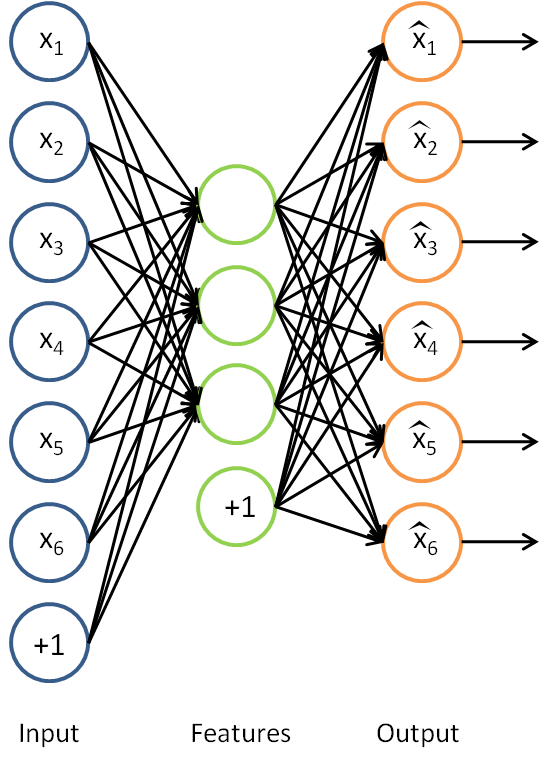
\includegraphics[width=0.4\textwidth]{figures/STL_SparseAE.png}
  %\caption{}\label{fig:zcawhiten}
\end{figure}

\cnt{Having trained the parameters $W^{(1)}, b^{(1)}, W^{(2)}, b^{(2)}$ of this model, given any new input $x$, we can now compute the corresponding vector of activations $a$ of the hidden units. As we saw previously, this often gives a better representation of the input than the original raw input $x$. We can also visualize the algorithm for computing the features/activations $a$ as the following neural network: }
    {利用训练得到的模型参数 $W^{(1)}, b^{(1)}, W^{(2)}, b^{(2)}$,给定任意的输入数据 $x$,可以计算隐藏单元的激活量(activations) $a$。如前所述,相比原始输入 $x$ 来说,$a$ 可能是一个更好的特征描述。下图的神经网络描述了特征(激活量 $a$)的计算。 }
    {}

\begin{figure}[ht] \centering
  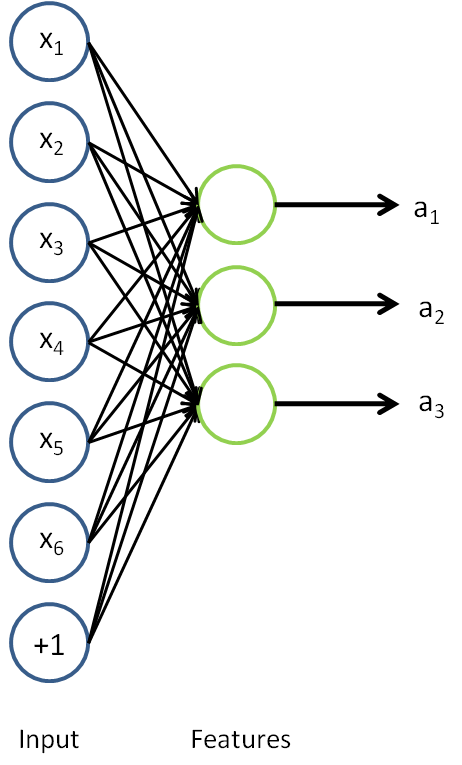
\includegraphics[width=0.4\textwidth]{figures/STL_SparseAE_Features.png}
  %\caption{}\label{fig:zcawhiten}
\end{figure}

\cnt{This is just the sparse autoencoder that we previously had, with with the final layer removed. }
    {这实际上就是之前得到的稀疏自编码器,在这里去掉了最后一层。}
    {}

\cnt{Now, suppose we have a labeled training set $\{ (x_l^{(1)}, y^{(1)}), (x_l^{(2)}, y^{(2)}), \ldots (x_l^{(m_l)}, y^{(m_l)}) \}$ of $m_l$ examples. (The subscript ``$l$" stands for ``labeled.") We can now find a better representation for the inputs. In particular, rather than representing the first training example as $x_l^{(1)}$, we can feed $x_l^{(1)}$ as the input to our autoencoder, and obtain the corresponding vector of activations $a_l^{(1)}$. To represent this example, we can either just \emph{replace} the original feature vector with $a_l^{(1)}$. Alternatively, we can \emph{concatenate} the two feature vectors together, getting a representation $(x_l^{(1)}, a_l^{(1)})$. }
    {假定有大小为 $m_l$ 的已标注训练集 $\{ (x_l^{(1)}, y^{(1)}), (x_l^{(2)}, y^{(2)}), \ldots (x_l^{(m_l)}, y^{(m_l)}) \}$(下标 $l$ 表示“带类标”),我们可以为输入数据找到更好的特征描述。例如,可以将 $x_l^{(1)}$ 输入到稀疏自编码器,得到隐藏单元激活量 $a_l^{(1)}$。接下来,可以直接使用 $a_l^{(1)}$ 来\emph{代替}原始数据 $x_l^{(1)}$ (“替代表示”,Replacement Representation)。也可以合二为一,使用新的向量 $(x_l^{(1)}, a_l^{(1)})$ 来代替原始数据 $x_l^{(1)}$ (“级联表示”,Concatenation Representation)。 }
    {}

\cnt{Thus, our training set now becomes $\{ (a_l^{(1)}, y^{(1)}), (a_l^{(2)}, y^{(2)}), \ldots (a_l^{(m_l)}, y^{(m_l)}) \}$ (if we use the replacement representation, and use $a_l^{(i)}$ to represent the $i$-th training example), or $\{ ((x_l^{(1)}, a_l^{(1)}), y^{(1)}), ((x_l^{(2)}, a_l^{(1)}), y^{(2)}), \ldots, ((x_l^{(m_l)}, a_l^{(1)}), y^{(m_l)}) \}$ (if we use the concatenated representation). In practice, the concatenated representation often works better; but for memory or computation representations, we will sometimes use the replacement representation as well. }
    {经过变换后,训练集就变成 $\{ (a_l^{(1)}, y^{(1)}), (a_l^{(2)}, y^{(2)}), \ldots (a_l^{(m_l)}, y^{(m_l)}) \}$ 或者是 $\{ ((x_l^{(1)}, a_l^{(1)}), y^{(1)}), ((x_l^{(2)}, a_l^{(1)}), y^{(2)}), \ldots, ((x_l^{(m_l)}, a_l^{(1)}), y^{(m_l)}) \}$(取决于使用 $a_l^{(1)}$ 替换 $x_l^{(1)}$ 还是将二者合并)。在实践中,将 $a_l^{(1)}$ 和 $x_l^{(1)}$ 合并通常表现的更好。但是考虑到内存和计算的成本,也可以使用替换操作。 }
    {}

\cnt{Finally, we can train a supervised learning algorithm such as an SVM, logistic regression, etc. to obtain a function that makes predictions on the $y$ values. Given a test example $x_{\rm test}$, we would then follow the same procedure: For feed it to the autoencoder to get $a_{\rm test}$. Then, feed either $a_{\rm test}$ or $(x_{\rm test}, a_{\rm test})$ to the trained classifier to get a prediction. }
    {最终,可以训练出一个有监督学习算法(例如 svm, logistic regression 等),得到一个判别函数对 $y$ 值进行预测。预测过程如下:给定一个测试样本 $x_{\rm test}$,重复之前的过程,将其送入稀疏自编码器,得到 $a_{\rm test}$。然后将 $a_{\rm test}$ (或者 $(x_{\rm test}, a_{\rm test})$ )送入分类器中,得到预测值。 }
    {}

\subsubsection{\cnt{On pre-processing the data}{数据预处理}{}}

\cnt{During the feature learning stage where we were learning from the unlabeled training set $\{ x_u^{(1)}, x_u^{(2)}, \ldots, x_u^{(m_u)}\}$, we may have computed various pre-processing parameters. For example, one may have computed a mean value of the data and subtracted off this mean to perform mean normalization, or used PCA to compute a matrix $U$ to represent the data as $U^Tx$ (or used PCA whitening or ZCA whitening). If this is the case, then it is important to save away these preprocessing parameters, and to use the same parameters during the labeled training phase and the test phase, so as to make sure we are always transforming the data the same way to feed into the autoencoder. In particular, if we have computed a matrix $U$ using the unlabeled data and PCA, we should keep the same matrix $U$ and use it to preprocess the labeled examples and the test data. We should not re-estimate a different $U$ matrix (or data mean for mean normalization, etc.) using the labeled training set, since that might result in a dramatically different pre-processing transformation, which would make the input distribution to the autoencoder very different from what it was actually trained on. }
    {在特征学习阶段,我们从未标注训练集 $\{ x_u^{(1)}, x_u^{(2)}, \ldots, x_u^{(m_u)}\}$ 中学习,这一过程中可能计算了各种数据预处理参数。例如计算数据均值并且对数据做均值标准化(mean normalization);或者对原始数据做主成分分析(PCA),然后将原始数据表示为 $U^Tx$ (又或者使用 PCA 白化或 ZCA 白化)。这样的话,有必要将这些参数保存起来,并且在后面的训练和测试阶段使用同样的参数,以保证数据进入稀疏自编码神经网络之前经过了同样的变换。例如,如果对未标注数据集进行PCA预处理,就必须将得到的矩阵 $U$ 保存起来,并且应用到有标注训练集和测试集上;而不能使用有标注训练集重新估计出一个不同的矩阵 $U$ (也不能重新计算均值并做均值标准化),否则的话可能得到一个完全不一致的数据预处理操作,导致进入自编码器的数据分布迥异于训练自编码器时的数据分布。 }
    {}

\subsubsection{\cnt{On the terminology of unsupervised feature learning }{无监督特征学习的术语}{}}

\cnt{There are two common unsupervised feature learning settings, depending on what type of unlabeled data you have. The more general and powerful setting is the \emph{self-taught learning} setting, which does not assume that your unlabeled data $x_u$ has to be drawn from the same distribution as your labeled data $x_l$. The more restrictive setting where the unlabeled data comes from exactly the same distribution as the labeled data is sometimes called the \emph{semi-supervised learning} setting. This distinctions is best explained with an example, which we now give. }
    {有两种常见的无监督特征学习方式,区别在于你有什么样的未标注数据。\emph{自学习}(self-taught learning) 是其中更为一般的、更强大的学习方式,它不要求未标注数据 $x_u$ 和已标注数据 $x_l$ 来自同样的分布。另外一种带限制性的方式也被称为\emph{半监督学习},它要求 $x_u$ 和 $x_l$ 服从同样的分布。下面通过例子解释二者的区别。 }
    {}

\cnt{Suppose your goal is a computer vision task where you'd like to distinguish between images of cars and images of motorcycles; so, each labeled example in your training set is either an image of a car or an image of a motorcycle. Where can we get lots of unlabeled data? The easiest way would be to obtain some random collection of images, perhaps downloaded off the internet. We could then train the autoencoder on this large collection of images, and obtain useful features from them. Because here the unlabeled data is drawn from a different distribution than the labeled data (i.e., perhaps some of our unlabeled images may contain cars/motorcycles, but not every image downloaded is either a car or a motorcycle), we call this self-taught learning. }
    {假定有一个计算机视觉方面的任务,目标是区分汽车和摩托车图像;也即训练样本里面要么是汽车的图像,要么是摩托车的图像。哪里可以获取大量的未标注数据呢?最简单的方式可能是从互联网上下载一些随机的图像数据集,在这些数据上训练出一个稀疏自编码器,从中得到有用的特征。这个例子里,未标注数据完全来自于一个和已标注数据不同的分布(未标注数据集中,或许其中一些图像包含汽车或者摩托车,但是不是所有的图像都如此)。这种情形被称为自学习。 }
    {}

\cnt{In contrast, if we happen to have lots of unlabeled images lying around that are all images of either a car or a motorcycle, but where the data is just missing its label (so you don't know which ones are cars, and which ones are motorcycles), then we could use this form of unlabeled data to learn the features. This setting---where each unlabeled example is drawn from the same distribution as your labeled examples---is sometimes called the semi-supervised setting. In practice, we often do not have this sort of unlabeled data (where would you get a database of images where every image is either a car or a motorcycle, but just missing its label?), and so in the context of learning features from unlabeled data, the self-taught learning setting is more broadly applicable. }
    {相反,如果有大量的未标注图像数据,要么是汽车图像,要么是摩托车图像,仅仅是缺失了类标号(没有标注每张图片到底是汽车还是摩托车)。也可以用这些未标注数据来学习特征。这种方式,即要求未标注样本和带标注样本服从相同的分布,有时候被称为半监督学习。在实践中,常常无法找到满足这种要求的未标注数据(到哪里找到一个每张图像不是汽车就是摩托车,只是丢失了类标号的图像数据库?)因此,自学习在无标注数据集的特征学习中应用更广。 }
    {}

\subsection{\cnt{Exercise: Self-Taught Learning}{练习:自学习}{}} \label{chp:execselftaughtlearn}

\subsubsection{\cnt{Overview}{综述}{}}

\cnt{In this exercise, we will use the self-taught learning paradigm with the sparse autoencoder and softmax classifier to build a classifier for handwritten digits. }
    {}
    {}


\cnt{You will be building upon your code from the earlier exercises. First, you will train your sparse autoencoder on an ``unlabeled" training dataset of handwritten digits. This produces feature that are penstroke-like. We then extract these learned features from a labeled dataset of handwritten digits. These features will then be used as inputs to the softmax classifier that you wrote in the previous exercise. }
    {}
    {}


\cnt{Concretely, for each example in the the labeled training dataset $x_l$, we forward propagate the example to obtain the activation of the hidden units $a^{(2)}$. We now represent this example using $a^{(2)}$ (the ``replacement" representation), and use this to as the new feature representation with which to train the softmax classifier. }
    {}
    {}


\cnt{Finally, we also extract the same features from the test data to obtain predictions.}
    {}
    {}

\cnt{In this exercise, our goal is to distinguish between the digits from 0 to 4. We will use the digits 5 to 9 as our ``unlabeled" dataset which which to learn the features; we will then use a labeled dataset with the digits 0 to 4 with which to train the softmax classifier.}
    {}
    {}

\cnt{In the starter code, we have provided a file \texttt{stlExercise.m} that will help walk you through the steps in this exercise. }
    {}
    {}

\subsubsection{\cnt{Dependencies}{}{}}

\cnt{The following additional files are required for this exercise: }
    {}
    {}
\begin{itemize}
  \item MNIST Dataset \url{http://yann.lecun.com/exdb/mnist/}
  \item Support functions for loading MNIST in Matlab (\ref{chp:usemnistdata})
  \item Starter Code \href{http://ufldl.stanford.edu/wiki/resources/stl_exercise.zip}{stl\_exercise.zip}) 
\end{itemize}

\cnt{You will also need your code from the following exercises: }
    {}
    {}
\begin{itemize}
  \item Exercise:Sparse Autoencoder (\ref{chp:execsparseautoenc})
  \item Exercise:Vectorization (\ref{chp:vecexec})
  \item Exercise:Softmax Regression (\ref{chp:execsoftmaxreg})
\end{itemize}

\emph{
\cnt{If you have not completed the exercises listed above, we strongly suggest you complete them first.}
    {}
    {}
}

\subsubsection{\cnt{Step 1: Generate the input and test data sets}{}{}}

\cnt{Download and decompress \href{http://ufldl.stanford.edu/wiki/resources/stl_exercise.zip}{stl\_exercise.zip}, which contains starter code for this exercise. Additionally, you will need to download the datasets from the MNIST Handwritten Digit Database for this project. }
    {}
    {}

\subsubsection{\cnt{Step 2: Train the sparse autoencoder}{}{}}

\cnt{Next, use the unlabeled data (the digits from 5 to 9) to train a sparse autoencoder, using the same \texttt{sparseAutoencoderCost.m} function as you had written in the previous exercise. (From the earlier exercise, you should have a working and vectorized implementation of the sparse autoencoder.) For us, the training step took less than 25 minutes on a fast desktop. When training is complete, you should get a visualization of pen strokes like the image shown below: }
    {}
    {}

\begin{figure}[ht] \centering
  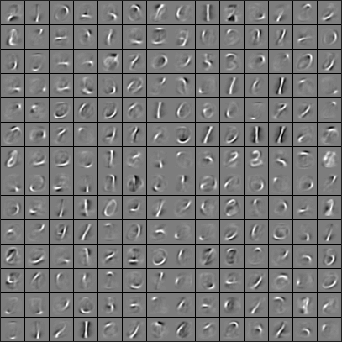
\includegraphics[width=0.5\textwidth]{figures/SelfTaughtFeatures.png}
  %\caption{}\label{fig:step1}
\end{figure}

\cnt{Informally, the features learned by the sparse autoencoder should correspond to penstrokes. }
    {}
    {}

\subsubsection{\cnt{Step 3: Extracting features}{}{}}

\cnt{After the sparse autoencoder is trained, you will use it to extract features from the handwritten digit images.}
    {}
    {}

\cnt{Complete \texttt{feedForwardAutoencoder.m} to produce a matrix whose columns correspond to activations of the hidden layer for each example, i.e., the vector $a^{(2)}$ corresponding to activation of layer 2. (Recall that we treat the inputs as layer 1).}
    {}
    {}

\cnt{After completing this step, calling \texttt{feedForwardAutoencoder.m} should convert the raw image data to hidden unit activations $a^{(2)}$.}
    {}
    {}

\subsubsection{\cnt{Step 4: Training and testing the logistic regression model}{}{}}

\cnt{Use your code from the softmax exercise (\texttt{softmaxTrain.m}) to train a softmax classifier using the training set features (\texttt{trainFeatures}) and labels (\texttt{trainLabels}). }
    {}
    {}

\subsubsection{\cnt{Step 5: Classifying on the test set}{}{}}

\cnt{Finally, complete the code to make predictions on the test set (\texttt{testFeatures}) and see how your learned features perform! If you've done all the steps correctly, you should get an accuracy of about 98\% percent. }
    {}
    {}

\cnt{As a comparison, when \emph{raw pixels} are used (instead of the learned features), we obtained a test accuracy of only around 96\% (for the same train and test sets). }
    {}
    {}


\clearpage
%# -*- coding: utf-8 -*-
%!TEX encoding = UTF-8 Unicode
%!TEX TS-program = xelatex
% vim:ts=4:sw=4
%
% 以上设定默认使用 XeLaTex 编译,并指定 Unicode 编码,供 TeXShop 自动识别

% Author: Yunhui Fu <yhfudev@gmail.com>
% License: Creative Commons (CC BY 4.0)

\clearpage
\section{\cnt{Building Deep Networks for Classification}{建立分类用深度网络}{}}

\subsection{\cnt{From Self-Taught Learning to Deep Networks}{从自我学习到深层网络}{}}

\cnt{In the previous section(\ref{chp:selftaughtlearning}), you used an autoencoder to learn features that were then fed as input to a softmax or logistic regression classifier. In that method, the features were learned using only unlabeled data. In this section, we describe how you can \emph{fine-tune} and further improve the learned features using labeled data. When you have a large amount of labeled training data, this can significantly improve your classifier's performance. }
    {在前一节(\ref{chp:selftaughtlearning})中,我们利用自编码器来学习输入至 softmax 或 logistic 回归分类器的特征。这些特征仅利用未标注数据学习获得。在本节中,我们描述如何利用已标注数据进行\emph{微调},从而进一步优化这些特征。如果有大量已标注数据,通过微调就可以显著提升分类器的性能。 }
    {}


\cnt{In self-taught learning, we first trained a sparse autoencoder on the unlabeled data. Then, given a new example $x$, we used the hidden layer to extract features $a$. This is illustrated in the following diagram: }
    {在自我学习中,我们首先利用未标注数据训练一个稀疏自编码器。随后,给定一个新样本 $x$,我们通过隐含层提取出特征 $a$。上述过程图示如下: }
    {}

% duplicated figure:
\begin{figure}[ht] \centering
  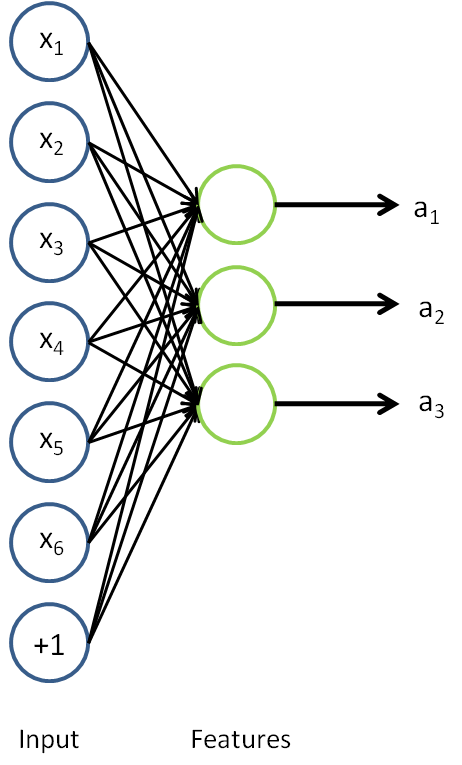
\includegraphics[width=0.4\textwidth]{figures/STL_SparseAE_Features.png}
  %\caption{}\label{fig:step1}
\end{figure}

\cnt{We are interested in solving a classification task, where our goal is to predict labels $y$. We have a labeled training set $\{ (x_l^{(1)}, y^{(1)}), (x_l^{(2)}, y^{(2)}), \ldots (x_l^{(m_l)}, y^{(m_l)}) \}$ of $m_l$ labeled examples. We showed previously that we can replace the original features $x^{(i)}$ with features $a^{(l)}$ computed by the sparse autoencoder (the ``replacement" representation). This gives us a training set $\{(a^{(1)}, y^{(1)}), \ldots (a^{(m_l)}, y^{(m_l)}) \}$. Finally, we train a logistic classifier to map from the features $a^{(i)}$ to the classification label $y^{(i)}$. To illustrate this step, similar to our earlier notes(\ref{chp:neuralnet}), we can draw our logistic regression unit (shown in orange) as follows: }
    {我们感兴趣的是分类问题,目标是预测样本的类别标号 $y$。我们拥有标注数据集 $\{ (x_l^{(1)}, y^{(1)}), (x_l^{(2)}, y^{(2)}), \ldots (x_l^{(m_l)},y^{(m_l)}) \}$,包含 $m_l$ 个标注样本。此前我们已经说明,可以利用稀疏自编码器获得的特征 $a^{(l)}$ 来替代原始特征。这样就可获得训练数据集 $\{(a^{(1)},y^{(1)}), \ldots (a^{(m_l)}, y^{(m_l)}) \}$。最终,我们训练出一个从特征 $a^{(i)}$ 到类标号 $y^{(i)}$ 的 logistic 分类器。为说明这一过程,我们按照神经网络一节(\ref{chp:neuralnet})中的方式,用下图描述 logistic 回归单元(橘黄色)。 }
    {}

\begin{figure}[ht] \centering
  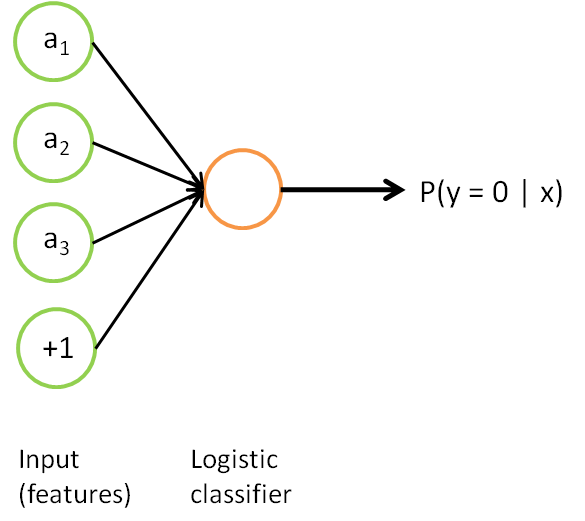
\includegraphics[width=0.5\textwidth]{figures/STL_Logistic_Classifier.png}
  %\caption{}\label{fig:step1}
\end{figure}

\cnt{Now, consider the overall classifier (i.e., the input-output mapping) that we have learned using this method. In particular, let us examine the function that our classifier uses to map from from a new test example $x$ to a new prediction $p(y = 1 | x)$. We can draw a representation of this function by putting together the two pictures from above. In particular, the final classifier looks like this:}
    {考虑利用这个方法所学到的分类器(输入-输出映射)。它描述了一个把测试样本 $x$ 映射到预测值 $p(y=1|x)$ 的函数。将此前的两张图片结合起来,就得到该函数的图形表示。也即,最终的分类器可以表示为: }
    {}

\begin{figure}[ht] \centering
  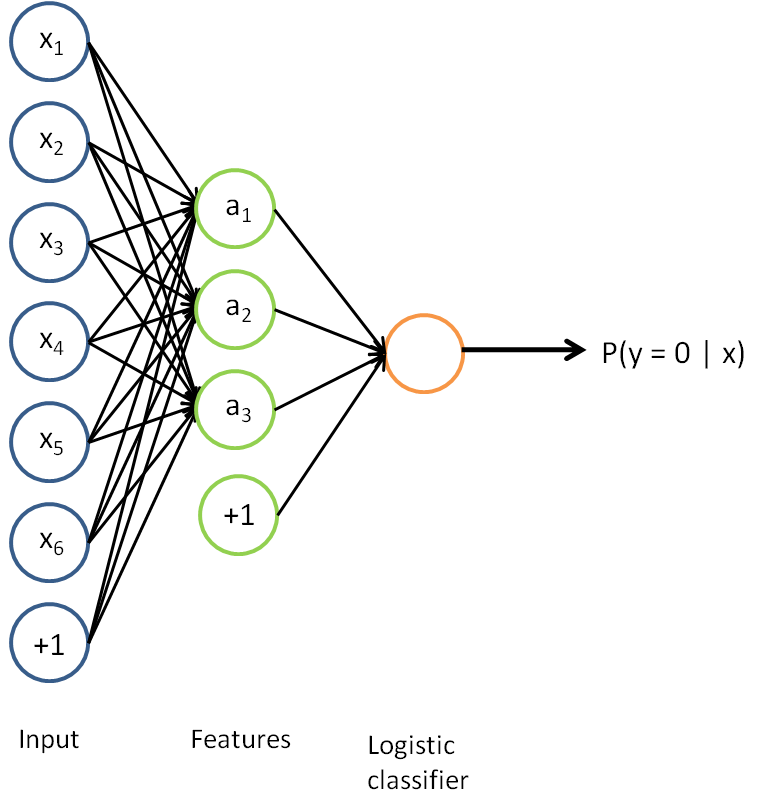
\includegraphics[width=0.57\textwidth]{figures/STL_CombinedAE.png}
  %\caption{}\label{fig:step1}
\end{figure}

\cnt{The parameters of this model were trained in two stages: The first layer of weights $W^{(1)}$ mapping from the input $x$ to the hidden unit activations $a$ were trained as part of the sparse autoencoder training process. The second layer of weights $W^{(2)}$ mapping from the activations $a$ to the output $y$ was trained using logistic regression (or softmax regression). }
    {该模型的参数通过两个步骤训练获得:在该网络的第一层,将输入 $x$ 映射至隐藏单元激活量 $a$ 的权值 $W^{(1)}$ 可以通过稀疏自编码器训练过程获得。在第二层,将隐藏单元 $a$ 映射至输出 $y$ 的权值 $W^{(2)}$ 可以通过 logistic 回归或 softmax 回归训练获得。}
    {}

\cnt{But the form of our overall/final classifier is clearly just a whole big neural network. So, having trained up an initial set of parameters for our model (training the first layer using an autoencoder, and the second layer via logistic/softmax regression), we can further modify all the parameters in our model to try to further reduce the training error. In particular, we can fine-tune the parameters, meaning perform gradient descent (or use L-BFGS) from the current setting of the parameters to try to reduce the training error on our labeled training set $\{ (x_l^{(1)}, y^{(1)}), (x_l^{(2)}, y^{(2)}), \ldots (x_l^{(m_l)}, y^{(m_l)}) \}$. }
    {这个最终分类器整体上显然是一个大的神经网络。因此,在训练获得模型最初参数(利用自动编码器训练第一层,利用 logistic/softmax 回归训练第二层)之后,我们可以进一步修正模型参数,进而降低训练误差。具体来说,我们可以对参数进行微调,在现有参数的基础上采用梯度下降或者 L-BFGS 来降低已标注样本集 $\{ (x_l^{(1)}, y^{(1)}), (x_l^{(2)}, y^{(2)}), \ldots (x_l^{(m_l)}, y^{(m_l)}) \}$ 上的训练误差。}
    {}

\cnt{When fine-tuning is used, sometimes the original unsupervised feature learning steps (i.e., training the autoencoder and the logistic classifier) are called \emph{pre-training}. The effect of fine-tuning is that the labeled data can be used to modify the weights $W^{(1)}$ as well, so that adjustments can be made to the features $a$ extracted by the layer of hidden units.}
    {使用微调时,初始的非监督特征学习步骤(也就是自动编码器和logistic分类器训练)有时候被称为\emph{预训练}。微调的作用在于,已标注数据集也可以用来修正权值 $W^{(1)}$,这样可以对隐藏单元所提取的特征 $a$ 做进一步调整。}
    {}

\cnt{So far, we have described this process assuming that you used the ``replacement" representation, where the training examples seen by the logistic classifier are of the form $(a^{(i)}, y^{(i)})$, rather than the ``concatenation" representation, where the examples are of the form $((x^{(i)}, a^{(i)}), y^{(i)})$. It is also possible to perform fine-tuning too using the ``concatenation" representation. (This corresponds to a neural network where the input units $x_i$ also feed directly to the logistic classifier in the output layer. You can draw this using a slightly different type of neural network diagram than the ones we have seen so far; in particular, you would have edges that go directly from the first layer input nodes to the third layer output node, ``skipping over" the hidden layer.) However, so long as we are using finetuning, usually the ``concatenation" representation has little advantage over the ``replacement" representation. Thus, if we are using fine-tuning usually we will do so with a network built using the replacement representation. (If you are not using fine-tuning however, then sometimes the concatenation representation can give much better performance.)}
    {到现在为止,我们描述上述过程时,都假设采用了“替代 (Replacement)”表示而不是“级联 (Concatenation)”表示。在替代表示中,logistic 分类器所看到的训练样本格式为 $(a^{(i)}, y^{(i)})$;而在级联表示中,分类器所看到的训练样本格式为 $((x^{(i)}, a^{(i)}), y^{(i)})$。对级联表示同样可以进行微调(在级联表示神经网络中,输入值 $x_i$ 也直接被输入至 logistic 分类器。对此前的神经网络示意图稍加更改,即可获得其示意图。具体的说,第一层的输入节点除了与隐层联接之外,还将越过隐层,与第三层输出节点直接相连)。但是对于微调来说,级联表示相对于替代表示几乎没有优势。因此,如果需要开展微调,我们通常使用替代表示的网络(但是如果不开展微调,级联表示的效果有时候会好得多)。}
    {}

\cnt{When should we use fine-tuning? It is typically used only if you have a large labeled training set; in this setting, fine-tuning can significantly improve the performance of your classifier. However, if you have a large \emph{unlabeled} dataset (for unsupervised feature learning/pre-training) and only a relatively small labeled training set, then fine-tuning is significantly less likely to help.}
    {在什么时候应用微调?通常仅在有大量已标注训练数据的情况下使用。在这样的情况下,微调能显著提升分类器性能。然而,如果有大量\emph{未标注}数据集(用于非监督特征学习/预训练),却只有相对较少的已标注训练集,微调的作用非常有限。}
    {}

\subsection{\cnt{Deep Networks: Overview}{深度网络概览}{}}


\subsubsection{\cnt{Overview}{概览}{}}

\cnt{In the previous sections, you constructed a 3-layer neural network comprising an input, hidden and output layer. While fairly effective for MNIST, this 3-layer model is a fairly \emph{shallow} network; by this, we mean that the features (hidden layer activations ${a}^{(2)}$) are computed using only ``one layer" of computation (the hidden layer).}
    {在之前的章节中,你已经构建了一个包括输入层、隐藏层以及输出层的三层神经网络。虽然该网络对于MNIST手写数字数据库非常有效,但是它还是一个非常“\emph{浅}”的网络。这里的“浅”指的是特征(隐藏层的激活值 ${a}^{(2)}$)只使用一层计算单元(隐藏层)来得到的。}
    {}

\cnt{In this section, we begin to discuss \emph{deep} neural networks, meaning ones in which we have multiple hidden layers; this will allow us to compute much more complex features of the input. Because each hidden layer computes a non-linear transformation of the previous layer, a deep network can have significantly greater representational power (i.e., can learn significantly more complex functions) than a shallow one.}
    {在本节中,我们开始讨论\emph{深度}神经网络,即含有多个隐藏层的神经网络。通过引入深度网络,我们可以计算更多复杂的输入特征。因为每一个隐藏层可以对上一层的输出进行非线性变换,因此深度神经网络拥有比“浅层”网络更加优异的表达能力(例如可以学习到更加复杂的函数关系)。}
    {}

\cnt{Note that when training a deep network, it is important to use a \emph{non-linear} activation function $f(\cdot)$ in each hidden layer. This is because multiple layers of linear functions would itself compute only a linear function of the input (i.e., composing multiple linear functions together results in just another linear function), and thus be no more expressive than using just a single layer of hidden units.}
    {值得注意的是当训练深度网络的时候,每一层隐层应该使用\emph{非线性}的激活函数 $f(\cdot)$。这是因为多层的线性函数组合在一起本质上也只有线性函数的表达能力(例如,将多个线性方程组合在一起仅仅产生另一个线性方程)。因此,在激活函数是线性的情况下,相比于单隐藏层神经网络,包含多隐藏层的深度网络并没有增加表达能力。}
    {}

\subsubsection{\cnt{Advantages of deep networks}{深度网络的优势}{}}

\cnt{Why do we want to use a deep network? The primary advantage is that it can compactly represent a significantly larger set of fuctions than shallow networks. Formally, one can show that there are functions which a $k$-layer network can represent compactly (with a number of hidden units that is \emph{polynomial} in the number of inputs), that a $(k - 1)$-layer network cannot represent unless it has an exponentially large number of hidden units.}
    {为什么我们要使用深度网络呢?使用深度网络最主要的优势在于,它能以更加紧凑简洁的方式来表达比浅层网络大得多的函数集合。正式点说,我们可以找到一些函数,这些函数可以用 $k$ 层网络简洁地表达出来(这里的简洁是指隐层单元的数目只需与输入单元数目呈\emph{多项式关系})。但是对于一个只有 $k-1$ 层的网络而言,除非它使用与输入单元数目呈指数关系的隐层单元数目,否则不能简洁表达这些函数。}
    {}

\cnt{To take a simple example, consider building a boolean circuit/network to compute the parity (or XOR) of $n$ input bits. Suppose each node in the network can compute either the logical OR of its inputs (or the OR of the negation of the inputs), or compute the logical AND. If we have a network with only one input, one hidden, and one output layer, the parity function would require a number of nodes that is exponential in the input size $n$. If however we are allowed a deeper network, then the network/circuit size can be only polynomial in n.}
    {举一个简单的例子,比如我们打算构建一个布尔网络来计算 $n$ 个输入比特的奇偶校验码(或者进行异或运算)。假设网络中的每一个节点都可以进行逻辑“或”运算(或者“与非”运算),亦或者逻辑“与”运算。如果我们拥有一个仅仅由一个输入层、一个隐层以及一个输出层构成的网络,那么该奇偶校验函数所需要的节点数目与输入层的规模 $n$ 呈指数关系。但是,如果我们构建一个更深点的网络,那么这个网络的规模就可做到仅仅是 $n$ 的多项式函数。}
    {}


\cnt{By using a deep network, in the case of images, one can also start to learn part-whole decompositions. For example, the first layer might learn to group together pixels in an image in order to detect edges (as seen in the earlier exercises). The second layer might then group together edges to detect longer contours, or perhaps detect simple ``parts of objects." An even deeper layer might then group together these contours or detect even more complex features.}
    {当处理对象是图像时,我们能够使用深度网络学习到“部分-整体”的分解关系。例如,第一层可以学习如何将图像中的像素组合在一起来检测边缘(正如我们在前面的练习中做的那样)。第二层可以将边缘组合起来检测更长的轮廓或者简单的“目标的部件”。在更深的层次上,可以将这些轮廓进一步组合起来以检测更为复杂的特征。}
    {}


\cnt{Finally, cortical computations (in the brain) also have multiple layers of processing. For example, visual images are processed in multiple stages by the brain, by cortical area ``V1", followed by cortical area ``V2" (a different part of the brain), and so on.}
    {最后要提的一点是,大脑皮层同样是分多层进行计算的。例如视觉图像在人脑中是分多个阶段进行处理的,首先是进入大脑皮层的“V1”区,然后紧跟着进入大脑皮层“V2”区,以此类推。}
    {}


\subsubsection{\cnt{Difficulty of training deep architectures}{训练深度网络的困难}{}}


\cnt{While the theoretical benefits of deep networks in terms of their compactness and expressive power have been appreciated for many decades, until recently researchers had little success training deep architectures.}
    {虽然几十年前人们就发现了深度网络在理论上的简洁性和较强的表达能力,但是直到最近,研究者们也没有在训练深度网络方面取得多少进步。}
    {}


\cnt{The main learning algorithm that researchers were using was to randomly initialize the weights of a deep network, and then train it using a labeled training set $\{ (x^{(1)}_l, y^{(1)}), \ldots, (x^{(m_l)}_l, y^{(m_l)}) \}$ using a supervised learning objective, for example by applying gradient descent to try to drive down the training error. However, this usually did not work well. There were several reasons for this.}
    {问题原因在于研究者们主要使用的学习算法是:首先随机初始化深度网络的权重,然后使用有监督的目标函数在有标签的训练集 $\left\{ \left( x_{l}^{\left( 1 \right)},{{y}^{\left( 1 \right)}} \right), \ldots, \left( x_{l}^{\left( {{m}_{l}} \right)},{{y}^{\left( {{m}_{l}} \right)}} \right) \right\}$ 上进行训练。例如通过使用梯度下降法来降低训练误差。然而,这种方法通常不是十分奏效。这其中有如下几方面原因:}
    {}



\textbf{\cnt{Availability of data}{数据获取问题}{}}


\cnt{With the method described above, one relies only on labeled data for training. However, labeled data is often scarce, and thus for many problems it is difficult to get enough examples to fit the parameters of a complex model. For example, given the high degree of expressive power of deep networks, training on insufficient data would also result in overfitting.}
    {使用上面提到的方法,我们需要依赖于有标签的数据才能进行训练。然而有标签的数据通常是稀缺的,因此对于许多问题,我们很难获得足够多的样本来拟合一个复杂模型的参数。例如,考虑到深度网络具有强大的表达能力,在不充足的数据上进行训练将会导致过拟合。}
    {}


\textbf{\cnt{Local optima}{局部极值问题}{}}


\cnt{Training a shallow network (with 1 hidden layer) using supervised learning usually resulted in the parameters converging to reasonable values; but when we are training a deep network, this works much less well. In particular, training a neural network using supervised learning involves solving a highly non-convex optimization problem (say, minimizing the training error $\sum_i ||h_W(x^{(i)}) - y^{(i)}||^2$ as a function of the network parameters $W$). In a deep network, this problem turns out to be rife with bad local optima, and training with gradient descent (or methods like conjugate gradient and L-BFGS) no longer work well.}
    {使用监督学习方法来对浅层网络(只有一个隐藏层)进行训练通常能够使参数收敛到合理的范围内。但是当用这种方法来训练深度网络的时候,并不能取得很好的效果。特别的,使用监督学习方法训练神经网络时,通常会涉及到求解一个高度非凸的优化问题(例如最小化训练误差 $\sum\nolimits_{i}{||{{h}_{W}}\left( {{x}^{\left( i \right)}} \right)-{{y}^{\left( i \right)}}|{{|}^{2}}}$,其中参数 $W$ 是要优化的参数。对深度网络而言,这种非凸优化问题的搜索区域中充斥着大量“坏”的局部极值,因而使用梯度下降法(或者像共轭梯度下降法,L-BFGS等方法)效果并不好。}
    {}


\textbf{\cnt{Diffusion of gradients}{梯度弥散问题}{}}

\cnt{There is an additional technical reason, pertaining to the gradients becoming very small, that explains why gradient descent (and related algorithms like L-BFGS) do not work well on a deep networks with randomly initialized weights. Specifically, when using backpropagation to compute the derivatives, the gradients that are propagated backwards (from the output layer to the earlier layers of the network) rapidly diminish in magnitude as the depth of the network increases. As a result, the derivative of the overall cost with respect to the weights in the earlier layers is very small. Thus, when using gradient descent, the weights of the earlier layers change slowly, and the earlier layers fail to learn much. This problem is often called the ``diffusion of gradients."}
    {梯度下降法(以及相关的L-BFGS算法等)在使用随机初始化权重的深度网络上效果不好的技术原因是:梯度会变得非常小。具体而言,当使用反向传播方法计算导数的时候,随着网络的深度的增加,反向传播的梯度(从输出层到网络的最初几层)的幅度值会急剧地减小。结果就造成了整体的损失函数相对于最初几层的权重的导数非常小。这样,当使用梯度下降法的时候,最初几层的权重变化非常缓慢,以至于它们不能够从样本中进行有效的学习。这种问题通常被称为“梯度的弥散”.}
    {}


\cnt{A closely related problem to the diffusion of gradients is that if the last few layers in a neural network have a large enough number of neurons, it may be possible for them to model the labeled data alone without the help of the earlier layers. Hence, training the entire network at once with all the layers randomly initialized ends up giving similar performance to training a shallow network (the last few layers) on corrupted input (the result of the processing done by the earlier layers).}
    {与梯度弥散问题紧密相关的问题是:当神经网络中的最后几层含有足够数量神经元的时候,可能单独这几层就足以对有标签数据进行建模,而不用最初几层的帮助。因此,对所有层都使用随机初始化的方法训练得到的整个网络的性能将会与训练得到的浅层网络(仅由深度网络的最后几层组成的浅层网络)的性能相似。}
    {}



\subsubsection{\cnt{Greedy layer-wise training}{逐层贪婪训练方法}{}}



\cnt{How can we train a deep network? One method that has seen some success is the \emph{greedy layer-wise training} method. We describe this method in detail in later sections, but briefly, the main idea is to train the layers of the network one at a time, so that we first train a network with 1 hidden layer, and only after that is done, train a network with 2 hidden layers, and so on. At each step, we take the old network with $k - 1$ hidden layers, and add an additional $k$-th hidden layer (that takes as input the previous hidden layer $k - 1$ that we had just trained). Training can either be supervised (say, with classification error as the objective function on each step), but more frequently it is unsupervised (as in an autoencoder; details to provided later). The weights from training the layers individually are then used to initialize the weights in the final/overall deep network, and only then is the entire architecture ``fine-tuned" (i.e., trained together to optimize the labeled training set error).}
    {那么,我们应该如何训练深度网络呢?\emph{逐层贪婪训练}方法是取得一定成功的一种方法。我们会在后面的章节中详细阐述这种方法的细节。简单来说,逐层贪婪算法的主要思路是每次只训练网络中的一层,即我们首先训练一个只含一个隐藏层的网络,仅当这层网络训练结束之后才开始训练一个有两个隐藏层的网络,以此类推。在每一步中,我们把已经训练好的前 $k-1$ 层固定,然后增加第 $k$ 层(也就是将我们已经训练好的前 $k-1$ 的输出作为输入)。每一层的训练可以是有监督的(例如,将每一步的分类误差作为目标函数),但更通常使用无监督方法(例如自动编码器,我们会在后边的章节中给出细节)。这些各层单独训练所得到的权重被用来初始化最终(或者说全部)的深度网络的权重,然后对整个网络进行“微调”(即把所有层放在一起来优化有标签训练集上的训练误差).}
    {}

\cnt{The success of greedy layer-wise training has been attributed to a number of factors:}
    {逐层贪婪的训练方法取得成功要归功于以下几方面:}
    {}

\textbf{\cnt{Availability of data}{数据获取}{}}


\cnt{While labeled data can be expensive to obtain, unlabeled data is cheap and plentiful. The promise of self-taught learning is that by exploiting the massive amount of unlabeled data, we can learn much better models. By using unlabeled data to learn a good initial value for the weights in all the layers $W^{(l)}$ (except for the final classification layer that maps to the outputs/predictions), our algorithm is able to learn and discover patterns from massively more amounts of data than purely supervised approaches. This often results in much better classifiers being learned.}
    {虽然获取有标签数据的代价是昂贵的,但获取大量的无标签数据是容易的。自学习方法(self-taught learning)的潜力在于它能通过使用大量的无标签数据来学习到更好的模型。具体而言,该方法使用无标签数据来学习得到所有层(不包括用于预测标签的最终分类层)${{W}^{(l)}}$ 的最佳初始权重。相比纯监督学习方法,这种自学习方法能够利用多得多的数据,并且能够学习和发现数据中存在的模式。因此该方法通常能够提高分类器的性能。}
    {}


\textbf{\cnt{Better local optima}{更好的局部极值}{}}

\cnt{After having trained the network on the unlabeled data, the weights are now starting at a better location in parameter space than if they had been randomly initialized. We can then further fine-tune the weights starting from this location. Empirically, it turns out that gradient descent from this location is much more likely to lead to a good local minimum, because the unlabeled data has already provided a significant amount of ``prior" information about what patterns there are in the input data.}
    {当用无标签数据训练完网络后,相比于随机初始化而言,各层初始权重会位于参数空间中较好的位置上。然后我们可以从这些位置出发进一步微调权重。从经验上来说,以这些位置为起点开始梯度下降更有可能收敛到比较好的局部极值点,这是因为无标签数据已经提供了大量输入数据中包含的模式的先验信息。}
    {}

\cnt{In the next section, we will describe the specific details of how to go about implementing greedy layer-wise training.}
    {在下一节中,我们将会具体阐述如何进行逐层贪婪训练。}
    {}


\subsection{\cnt{Stacked Autoencoders}{栈式自编码算法}{}}

\subsubsection{\cnt{Overview}{概述}{}}


\cnt{The greedy layerwise approach for pretraining a deep network works by training each layer in turn. In this page, you will find out how autoencoders can be ``stacked" in a greedy layerwise fashion for pretraining (initializing) the weights of a deep network.}
    {逐层贪婪训练法依次训练网络的每一层,进而预训练整个深度神经网络。在本节中,我们将会学习如何将自编码器“栈化”到逐层贪婪训练法中,从而预训练(或者说初始化)深度神经网络的权重。}
    {}


\cnt{A stacked autoencoder is a neural network consisting of multiple layers of sparse autoencoders in which the outputs of each layer is wired to the inputs of the successive layer. Formally, consider a stacked autoencoder with n layers. Using notation from the autoencoder section, let $W^{(k, 1)}, W^{(k, 2)}, b^{(k, 1)}, b^{(k, 2)}$ denote the parameters $W^{(1)}, W^{(2)}, b^{(1)}, b^{(2)}$ for kth autoencoder. Then the encoding step for the stacked autoencoder is given by running the encoding step of each layer in forward order:}
    {栈式自编码神经网络是一个由多层稀疏自编码器组成的神经网络,其前一层自编码器的输出作为其后一层自编码器的输入。对于一个 $n$ 层栈式自编码神经网络,我们沿用自编码器一章的各种符号,假定用 $W^{(k, 1)}, W^{(k, 2)}, b^{(k, 1)}, b^{(k, 2)}$ 表示第 $k$ 个自编码器对应的 $W^{(1)}, W^{(2)}, b^{(1)}, b^{(2)}$ 参数,那么该栈式自编码神经网络的编码过程就是,按照从前向后的顺序执行每一层自编码器的编码步骤:}
    {}

\begin{align} a^{(l)} = f(z^{(l)}) \\ z^{(l + 1)} = W^{(l, 1)}a^{(l)} + b^{(l, 1)} \end{align}

\cnt{The decoding step is given by running the decoding stack of each autoencoder in reverse order:}
    {同理,栈式神经网络的解码过程就是,按照从后向前的顺序执行每一层自编码器的解码步骤:}
    {}

\begin{align} a^{(n + l)} = f(z^{(n + l)}) \\ z^{(n + l + 1)} = W^{(n - l, 2)}a^{(n + l)} + b^{(n - l, 2)} \end{align}


\cnt{The information of interest is contained within $a^{(n)}$, which is the activation of the deepest layer of hidden units. This vector gives us a representation of the input in terms of higher-order features.}
    {其中,$a^{(n)}$ 是最深层隐藏单元的激活值,其包含了我们感兴趣的信息,这个向量也是对输入值的更高阶的表示。}
    {}


\cnt{The features from the stacked autoencoder can be used for classification problems by feeding $a^{(n)}$ to a softmax classifier.}
    {通过将 $a^{(n)}$ 作为softmax分类器的输入特征,可以将栈式自编码神经网络中学到的特征用于分类问题。}
    {}

\textbf{\cnt{Training}{训练}{}}


\cnt{A good way to obtain good parameters for a stacked autoencoder is to use greedy layer-wise training. To do this, first train the first layer on raw input to obtain parameters $W^{(1,1)}, W^{(1,2)}, b^{(1,1)}, b^{(1,2)}$. Use the first layer to transform the raw input into a vector consisting of activation of the hidden units, A. Train the second layer on this vector to obtain parameters $W^{(2,1)}, W^{(2,2)}, b^{(2,1)}, b^{(2,2)}$. Repeat for subsequent layers, using the output of each layer as input for the subsequent layer.}
    {一种比较好的获取栈式自编码神经网络参数的方法是采用逐层贪婪训练法进行训练。即先利用原始输入来训练网络的第一层,得到其参数 $W^{(1,1)}, W^{(1,2)}, b^{(1,1)}, b^{(1,2)}$;然后网络第一层将原始输入转化成为由隐藏单元激活值组成的向量(假设该向量为A),接着把A作为第二层的输入,继续训练得到第二层的参数 $W^{(2,1)}, W^{(2,2)}, b^{(2,1)}, b^{(2,2)}$;最后,对后面的各层同样采用的策略,即将前层的输出作为下一层输入的方式依次训练。}
    {}


\cnt{This method trains the parameters of each layer individually while freezing parameters for the remainder of the model. To produce better results, after this phase of training is complete, fine-tuning(Fine-tuning Stacked AEs \ref{chp:fintuningstkae}) using backpropagation can be used to improve the results by tuning the parameters of all layers are changed at the same time.}
    {对于上述训练方式,在训练每一层参数的时候,会固定其它各层参数保持不变。所以,如果想得到更好的结果,在上述预训练过程完成之后,可以通过反向传播算法同时调整所有层的参数以改善结果,这个过程一般被称作“微调(fine-tuning)”。
    实际上,使用逐层贪婪训练方法将参数训练到快要收敛时,应该使用微调(\ref{chp:fintuningstkae})。反之,如果直接在随机化的初始权重上使用微调,那么会得到不好的结果,因为参数会收敛到局部最优。}
    {}

\notes{
\cnt{If one is only interested in finetuning for the purposes of classification, the common practice is to then discard the ``decoding" layers of the stacked autoencoder and link the last hidden layer $a^{(n)}$ to the softmax classifier. The gradients from the (softmax) classification error will then be backpropagated into the encoding layers.}
    {如果你只对以分类为目的的微调感兴趣,那么惯用的做法是丢掉栈式自编码网络的“解码”层,直接把最后一个隐藏层的 $a^{(n)}$ 作为特征输入到softmax分类器进行分类,这样,分类器(softmax)的分类错误的梯度值就可以直接反向传播给编码层了。}
    {}
}

\textbf{\cnt{Concrete example}{具体实例}{}}


\cnt{To give a concrete example, suppose you wished to train a stacked autoencoder with 2 hidden layers for classification of MNIST digits, as you will be doing in the next exercise(\ref{chp:execdeepnetdigitclass}).}
    {让我们来看个具体的例子,假设你想要训练一个包含两个隐含层的栈式自编码网络,用来进行MNIST手写数字分类(这将会是你的下一个练习)。}
    {}


\cnt{First, you would train a sparse autoencoder on the raw inputs $x^{(k)}$ to learn primary features $h^{(1)(k)}$ on the raw input.}
    {首先,你需要用原始输入 $x^{(k)}$ 训练第一个自编码器,它能够学习得到原始输入的一阶特征表示 $h^{(1)(k)}$(如下图所示)。}
    {}

\begin{figure}[ht] \centering
  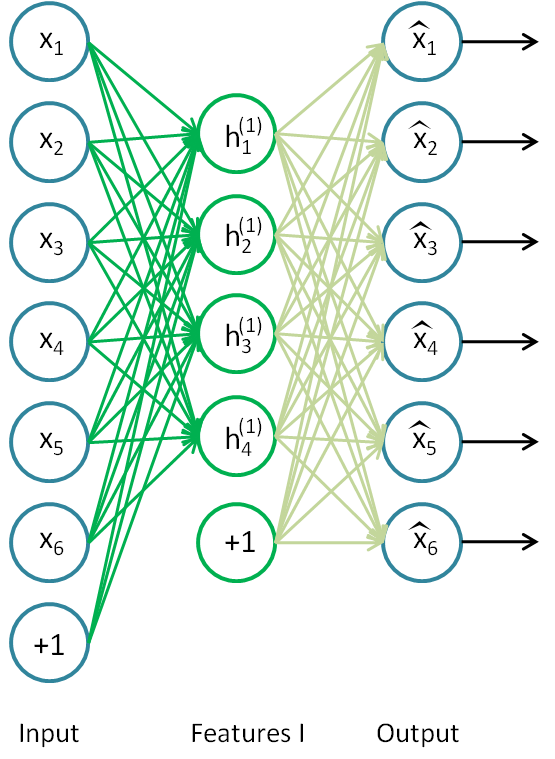
\includegraphics[width=0.5\textwidth]{figures/Stacked_SparseAE_Features1.png}
  %\caption{}\label{fig:step1}
\end{figure}


\cnt{Next, you would feed the raw input into this trained sparse autoencoder, obtaining the primary feature activations $h^{(1)(k)}$ for each of the inputs $x^{(k)}$. You would then use these primary features as the ``raw input" to another sparse autoencoder to learn secondary features $h^{(2)(k)}$ on these primary features.}
    {接着,你需要把原始数据输入到上述训练好的稀疏自编码器中,对于每一个输入 $x^{(k)}$,都可以得到它对应的一阶特征表示 $h^{(1)(k)}$。然后你再用这些一阶特征作为另一个稀疏自编码器的输入,使用它们来学习二阶特征 $h^{(2)(k)}$。(如下图所示)}
    {}


\begin{figure}[ht] \centering
  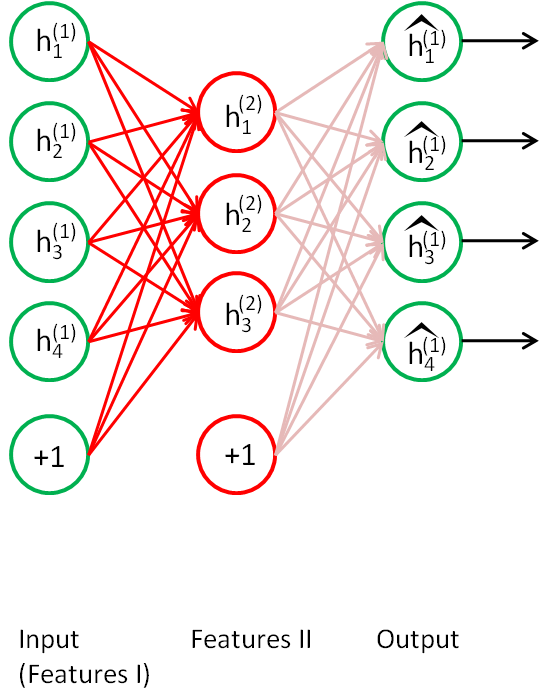
\includegraphics[width=0.5\textwidth]{figures/Stacked_SparseAE_Features2.png}
  %\caption{}\label{fig:step1}
\end{figure}

\cnt{Following this, you would feed the primary features into the second sparse autoencoder to obtain the secondary feature activations $h^{(2)(k)}$ for each of the primary features $h^{(1)(k)}$ (which correspond to the primary features of the corresponding inputs $x^{(k)}$). You would then treat these secondary features as ``raw input" to a softmax classifier, training it to map secondary features to digit labels.}
    {同样,再把一阶特征输入到刚训练好的第二层稀疏自编码器中,得到每个 $h^{(1)(k)}$ 对应的二阶特征激活值 $h^{(2)(k)}$。接下来,你可以把这些二阶特征作为softmax分类器的输入,训练得到一个能将二阶特征映射到数字标签的模型。}
    {}

\begin{figure}[ht] \centering
  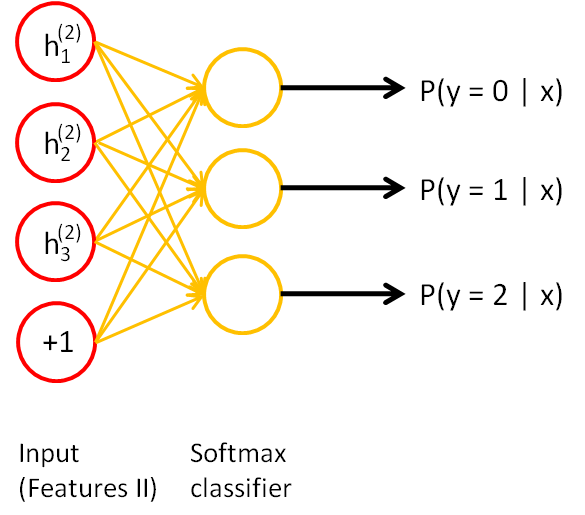
\includegraphics[width=0.5\textwidth]{figures/Stacked_Softmax_Classifier.png}
  %\caption{}\label{fig:step1}
\end{figure}

\cnt{Finally, you would combine all three layers together to form a stacked autoencoder with 2 hidden layers and a final softmax classifier layer capable of classifying the MNIST digits as desired.}
    {如下图所示,最终,你可以将这三层结合起来构建一个包含两个隐藏层和一个最终softmax分类器层的栈式自编码网络,这个网络能够如你所愿地对MNIST数字进行分类。}
    {}

\begin{figure}[ht] \centering
  \includegraphics[width=0.5\textwidth]{figures/Stacked_Combined.png}
  %\caption{}\label{fig:step1}
\end{figure}

\textbf{\cnt{Discussion}{讨论}{}}


\cnt{A stacked autoencoder enjoys all the benefits of any deep network of greater expressive power.}
    {栈式自编码神经网络具有强大的表达能力及深度神经网络的所有优点。}
    {}


\cnt{Further, it often captures a useful ``hierarchical grouping" or ``part-whole decomposition" of the input. To see this, recall that an autoencoder tends to learn features that form a good representation of its input. The first layer of a stacked autoencoder tends to learn first-order features in the raw input (such as edges in an image). The second layer of a stacked autoencoder tends to learn second-order features corresponding to patterns in the appearance of first-order features (e.g., in terms of what edges tend to occur together--for example, to form contour or corner detectors). Higher layers of the stacked autoencoder tend to learn even higher-order features.}
    {更进一步,它通常能够获取到输入的“层次型分组”或者“部分-整体分解”结构。为了弄清这一点,回顾一下,自编码器倾向于学习得到能更好地表示输入数据的特征。因此,栈式自编码神经网络的第一层会学习得到原始输入的一阶特征(比如图片里的边缘),第二层会学习得到二阶特征,该特征对应一阶特征里包含的一些模式(比如在构成轮廓或者角点时,什么样的边缘会共现)。栈式自编码神经网络的更高层还会学到更高阶的特征。举个例子,如果网络的输入数据是图像,网络的第一层会学习如何去识别边,第二层一般会学习如何去组合边,从而构成轮廓、角等。更高层会学习如何去组合更形象且有意义的特征。例如,如果输入数据集包含人脸图像,更高层会学习如何识别或组合眼睛、鼻子、嘴等人脸器官。}
    {}


\subsection{\cnt{Fine-tuning Stacked AEs}{微调多层自编码算法}{}} \label{chp:fintuningstkae}


\subsubsection{\cnt{Introduction}{介绍}{}}

\cnt{Fine tuning is a strategy that is commonly found in deep learning. As such, it can also be used to greatly improve the performance of a stacked autoencoder. From a high level perspective, fine tuning treats all layers of a stacked autoencoder as a single model, so that in one iteration, we are improving upon all the weights in the stacked autoencoder.}
    {微调是深度学习中的常用策略,可以大幅提升一个栈式自编码神经网络的性能表现。从更高的视角来讲,微调将栈式自编码神经网络的所有层视为一个模型,这样在每次迭代中,网络中所有的权重值都可以被优化。}
    {}


\subsubsection{\cnt{General Strategy}{一般策略}{}}

\cnt{Fortunately, we already have all the tools necessary to implement fine tuning for stacked autoencoders! In order to compute the gradients for all the layers of the stacked autoencoder in each iteration, we use the Backpropagation Algorithm(\ref{chp:bkpropgationalg}), as discussed in the sparse autoencoder section. As the backpropagation algorithm can be extended to apply for an arbitrary number of layers, we can actually use this algorithm on a stacked autoencoder of arbitrary depth.}
    {幸运的是,实施微调栈式自编码神经网络所需的工具都已齐备!为了在每次迭代中计算所有层的梯度,我们需要使用稀疏自动编码一节中讨论的反向传播算法(\ref{chp:bkpropgationalg})。因为反向传播算法可以延伸应用到任意多层,所以事实上,该算法对任意多层的栈式自编码神经网络都适用。}
    {}


\subsubsection{\cnt{Finetuning with Backpropagation}{使用反向传播法进行微调}{}}

\cnt{For your convenience, the summary of the backpropagation algorithm using element wise notation is below:}
    {为方便读者,以下我们简要描述如何实施反向传播算法:}
    {}

\begin{enumerate}
  \item
    \cnt{Perform a feedforward pass, computing the activations for layers $L_2$, $L_3$, up to the output layer $L_{n_l}$, using the equations defining the forward propagation steps.}
      {进行一次前馈传递,对 $L_2$ 层、$L_3$ 层直到输出层 $L_{n_l}$,使用前向传播步骤中定义的公式计算各层上的激活值(激励响应)。}
      {}

  \item
    \cnt{For the output layer (layer $n_l$), set}
      {对输出层($n_l$ 层),令}
      {}

\begin{align} \delta^{(n_l)} = - (\nabla_{a^{n_l}}J) \bullet f'(z^{(n_l)}) \end{align} 
        \cnt{(When using softmax regression, the softmax layer has $\nabla J = \theta^T(I-P)$ where I is the input labels and P is the vector of conditional probabilities.)}
      {(当使用softmax分类器时,softmax层满足:$\nabla J = \theta^T(I-P)$,其中 $I$ 为输入数据对应的类别标签,$P$ 为条件概率向量。)}
      {}

  \item
    \cnt{For $l = n_l-1, n_l-2, n_l-3, \ldots, 2$; Set}
      {对 $l = n_l-1, n_l-2, n_l-3, \ldots, 2$; 令}
      {}

            \begin{align} \delta^{(l)} = \left((W^{(l)})^T \delta^{(l+1)}\right) \bullet f'(z^{(l)}) \end{align} 

  \item
    \cnt{Compute the desired partial derivatives:}
      {计算所需的偏导数:}
      {}

        \begin{align} \nabla_{W^{(l)}} J(W,b;x,y) &= \delta^{(l+1)} (a^{(l)})^T, \\ \nabla_{b^{(l)}} J(W,b;x,y) &= \delta^{(l+1)}. \end{align} 

    \begin{align} J(W,b) &= \left[ \frac{1}{m} \sum_{i=1}^m J(W,b;x^{(i)},y^{(i)}) \right] \end{align} 
\end{enumerate}

\cnt{Note: While one could consider the softmax classifier as an additional layer, the derivation above does not. Specifically, we consider the ``last layer" of the network to be the features that goes into the softmax classifier. Therefore, the derivatives (in Step 2) are computed using $\delta^{(n_l)} = - (\nabla_{a^{n_l}}J) \bullet f'(z^{(n_l)})$, where $\nabla J = \theta^T(I-P)$.}
    {注:我们可以认为输出层softmax分类器是附加上的一层,但是其求导过程需要单独处理。具体地说,网络“最后一层”的特征会进入softmax分类器。所以,第二步中的导数由 $\delta^{(n_l)} = - (\nabla_{a^{n_l}}J) \bullet f'(z^{(n_l)})$ 计算,其中 $\nabla J = \theta^T(I-P)$。}
    {}

\subsection{\cnt{Exercise: Implement deep networks for digit classification}{练习:实现数字分类的深度网络}{}} \label{chp:execdeepnetdigitclass}


\subsubsection{\cnt{Overview}{}{}}


\cnt{In this exercise, you will use a stacked autoencoder for digit classification. This exercise is very similar to the self-taught learning exercise, in which we trained a digit classifier using a autoencoder layer followed by a softmax layer. The only difference in this exercise is that we will be using two autoencoder layers instead of one and further finetune the two layers.}
    {}
    {}


\cnt{The code you have already implemented will allow you to stack various layers and perform layer-wise training. However, to perform fine-tuning, you will need to implement backpropogation through both layers. We will see that fine-tuning significantly improves the model's performance.}
    {}
    {}


\cnt{In the file \href{http://ufldl.stanford.edu/wiki/resources/stackedae_exercise.zip}{stackedae\_exercise.zip}, we have provided some starter code. You will need to complete the code in \texttt{stackedAECost.m}, \texttt{stackedAEPredict.m} and \texttt{stackedAEExercise.m}. We have also provided \texttt{params2stack.m} and \texttt{stack2params.m} which you might find helpful in constructing deep networks.}
    {}
    {}


\subsubsection{\cnt{Dependencies}{}{}}

\cnt{The following additional files are required for this exercise:}
    {}
    {}

\begin{itemize}
  \item MNIST Dataset \url{http://yann.lecun.com/exdb/mnist/}
  \item Support functions for loading MNIST in Matlab (\ref{chp:usemnistdata})
  \item Starter Code (\href{http://ufldl.stanford.edu/wiki/resources/stackedae_exercise.zip}{stackedae\_exercise.zip})
\end{itemize}


\cnt{You will also need your code from the following exercises:}
    {}
    {}
\begin{itemize}
  \item Exercise:Sparse Autoencoder (\ref{chp:execsparseautoenc})
  \item Exercise:Vectorization (\ref{chp:vecexec})
  \item Exercise:Softmax Regression (\ref{chp:execsoftmaxreg})
  \item Exercise:Self-Taught Learning (\ref{chp:execselftaughtlearn})
\end{itemize}

\emph{
\cnt{If you have not completed the exercises listed above, we strongly suggest you complete them first.}
    {}
    {}
}

\subsubsection{\cnt{Step 0: Initialize constants and parameters}{}{}}

\cnt{Open \texttt{stackedAEExercise.m}. In this step, we set meta-parameters to the same values that were used in previous exercise, which should produce reasonable results. You may to modify the meta-parameters if you wish.}
    {}
    {}


\subsubsection{\cnt{Step 1: Train the data on the first stacked autoencoder}{}{}}

\cnt{Train the first autoencoder on the training images to obtain its parameters. This step is identical to the corresponding step in the sparse autoencoder and STL assignments, complete this part of the code so as to learn a first layer of features using your \texttt{sparseAutoencoderCost.m} and \texttt{minFunc}.}
    {}
    {}


\subsubsection{\cnt{Step 2: Train the data on the second stacked autoencoder}{}{}}

\cnt{We first forward propagate the training set through the first autoencoder (using \texttt{feedForwardAutoencoder.m} that you completed in Exercise:Self-Taught Learning(\ref{chp:execselftaughtlearn}) ) to obtain hidden unit activations. These activations are then used to train the second sparse autoencoder. Since this is just an adapted application of a standard autoencoder, it should run similarly with the first. Complete this part of the code so as to learn a first layer of features using your \texttt{sparseAutoencoderCost.m} and \texttt{minFunc}.}
    {}
    {}

\cnt{This part of the exercise demonstrates the idea of greedy layerwise training with the same learning algorithm reapplied multiple times.}
    {}
    {}

\subsubsection{\cnt{Step 3: Train the softmax classifier on the L2 features}{}{}}

\cnt{Next, continue to forward propagate the L1 features through the second autoencoder (using \texttt{feedForwardAutoencoder.m}) to obtain the L2 hidden unit activations. These activations are then used to train the softmax classifier. You can either use \texttt{softmaxTrain.m} or directly use \texttt{softmaxCost.m} that you completed in Exercise:Softmax Regression(\ref{chp:execsoftmaxreg}) to complete this part of the assignment.}
    {}
    {}



\subsubsection{\cnt{Step 4: Implement fine-tuning}{}{}}

\cnt{To implement fine tuning, we need to consider all three layers as a single model. Implement \texttt{stackedAECost.m} to return the cost and gradient of the model. The cost function should be as defined as the log likelihood and a gradient decay term. The gradient should be computed using back-propagation as discussed earlier(\ref{chp:bkpropgationalg}). The predictions should consist of the activations of the output layer of the softmax model.}
    {}
    {}

\cnt{To help you check that your implementation is correct, you should also check your gradients on a synthetic small dataset. We have implemented \texttt{checkStackedAECost.m} to help you check your gradients. If this checks passes, you will have implemented fine-tuning correctly.}
    {}
    {}

\notes{
\cnt{\textbf{Note}: When adding the weight decay term to the cost, you should regularize only the softmax weights (do not regularize the weights that compute the hidden layer activations).}
    {}
    {}
}

\notes{
\cnt{\textbf{Implementation Tip}: It is always a good idea to implement the code modularly and check (the gradient of) each part of the code before writing the more complicated parts.}
    {}
    {}
}

\subsubsection{\cnt{Step 5: Test the model}{}{}}

\cnt{Finally, you will need to classify with this model; complete the code in \texttt{stackedAEPredict.m} to classify using the stacked autoencoder with a classification layer.}
    {}
    {}

\cnt{After completing these steps, running the entire script in stackedAETrain.m will perform layer-wise training of the stacked autoencoder, finetune the model, and measure its performance on the test set. If you've done all the steps correctly, you should get an accuracy of about 87.7\% before finetuning and 97.6\% after finetuning (for the 10-way classification problem).}
    {}
    {}



\clearpage
%# -*- coding: utf-8 -*-
%!TEX encoding = UTF-8 Unicode
%!TEX TS-program = xelatex
% vim:ts=4:sw=4
%
% 以上设定默认使用 XeLaTex 编译,并指定 Unicode 编码,供 TeXShop 自动识别

% Author: Yunhui Fu <yhfudev@gmail.com>
% License: Creative Commons (CC BY 4.0)

\section{\cnt{Linear Decoders with Autoencoders}{自编码线性解码器}{}}

\subsection{\cnt{Linear Decoders}{线性解码器}{}}

\subsubsection{\cnt{Sparse Autoencoder Recap}{稀疏自编码重述}{}} \label{chp:sparseautoencrecap}

\cnt{In the sparse autoencoder, we had 3 layers of neurons: an input layer, a hidden layer and an output layer. In our previous description of autoencoders (and of neural networks), every neuron in the neural network used the same activation function. In these notes, we describe a modified version of the autoencoder in which some of the neurons use a different activation function. This will result in a model that is sometimes simpler to apply, and can also be more robust to variations in the parameters.}
    {稀疏自编码器包含3层神经元,分别是输入层,隐含层以及输出层。 从前面(神经网络)自编码器描述可知,位于神经网络中的神经元都采用相同的激励函数。 在注解中,我们修改了自编码器定义,使得某些神经元采用不同的激励函数。这样得到的模型更容易应用,而且模型对参数的变化也更为鲁棒。 }
    {}

\cnt{Recall that each neuron (in the output layer) computed the following:}
    {回想一下,输出层神经元计算公式如下:}
    {}
\begin{align} z^{(3)} &= W^{(2)} a^{(2)} + b^{(2)} \\ a^{(3)} &= f(z^{(3)}) \end{align}

\cnt{where $a^{(3)}$ is the output. In the autoencoder, $a^{(3)}$ is our approximate reconstruction of the input $x = a^{(1)}$.}
    {其中 $a^{(3)}$ 是输出. 在自编码器中, $a^{(3)}$ 近似重构了输入 $x = a^{(1)}$。 }
    {}

\cnt{Because we used a sigmoid activation function for $f(z^{(3)})$, we needed to constrain or scale the inputs to be in the range $[0,1]$, since the sigmoid function outputs numbers in the range $[0,1]$. While some datasets like MNIST fit well with this scaling of the output, this can sometimes be awkward to satisfy. For example, if one uses PCA whitening, the input is no longer constrained to $[0,1]$ and it's not clear what the best way is to scale the data to ensure it fits into the constrained range.}
    {S 型激励函数输出范围是 $[0,1]$,当 $f(z^{(3)})$ 采用该激励函数时,就要对输入限制或缩放,使其位于 $[0,1]$ 范围中。一些数据集,比如 MNIST,能方便将输出缩放到 $[0,1]$ 中,但是很难满足对输入值的要求。比如, PCA 白化处理的输入并不满足 $[0,1]$ 范围要求,也不清楚是否有最好的办法可以将数据缩放到特定范围中。}
    {}


\subsubsection{\cnt{Linear Decoder}{线性解码器}{}}

\cnt{One easy fix for this problem is to set $a^{(3)} = z^{(3)}$. Formally, this is achieved by having the output nodes use an activation function that's the identity function $f(z) = z$, so that $a^{(3)} = f(z^{(3)}) = z^{(3)}$. This particular activation function $f(\cdot)$ is called the linear activation function (though perhaps ``identity activation function" would have been a better name). Note however that in the hidden layer of the network, we still use a sigmoid (or tanh) activation function, so that the hidden unit activations are given by (say) $a^{(2)} = \sigma(W^{(1)}x + b^{(1)})$, where $\sigma(\cdot)$ is the sigmoid function, x is the input, and $W^{(1)}$ and $b^{(1)}$ are the weight and bias terms for the hidden units. It is only in the output layer that we use the linear activation function.}
    {设定 $a^{(3)} = z^{(3)}$ 可以很简单的解决上述问题。从形式上来看,就是输出端使用恒等函数 $f(z) = z$ 作为激励函数,于是有 $a^{(3)} = f(z^{(3)}) = z^{(3)}$。我们称该特殊的激励函数为 线性激励函数 (称为恒等激励函数可能更好些)。
    需要注意,神经网络中隐含层的神经元依然使用S型(或者$\tanh$)激励函数。这样隐含单元的激励公式为 $a^{(2)} = \sigma(W^{(1)}x + b^{(1)})$,其中 $\sigma(\cdot)$ 是 S 型函数, $x$ 是输入, $W^{(1)}$ 和 $b^{(1)}$ 分别是隐单元的权重和偏差项。我们仅在输出层中使用线性激励函数。

一个 S 型或 $\tanh$ 隐含层以及线性输出层构成的自编码器,我们称为线性解码器。}
    {}

\cnt{An autoencoder in this configuration--with a sigmoid (or tanh) hidden layer and a linear output layer--is called a linear decoder. In this model, we have $\hat{x} = a^{(3)} = z^{(3)} = W^{(2)}a + b^{(2)}$. Because the output $\hat{x}$ is a now linear function of the hidden unit activations, by varying $W^{(2)}$, each output unit $a^{(3)}$ can be made to produce values greater than 1 or less than 0 as well. This allows us to train the sparse autoencoder real-valued inputs without needing to pre-scale every example to a specific range.}
    {在这个线性解码器模型中,$\hat{x} = a^{(3)} = z^{(3)} = W^{(2)}a + b^{(2)}$。因为输出 $\hat{x}$ 是隐单元激励输出的线性函数,改变 $W^{(2)}$ ,可以使输出值 $a^{(3)}$ 大于 1 或者小于 0。这使得我们可以用实值输入来训练稀疏自编码器,避免预先缩放样本到给定范围。}
    {}

\cnt{Since we have changed the activation function of the output units, the gradients of the output units also change. Recall that for each output unit, we had set set the error terms as follows:}
    {随着输出单元的激励函数的改变,这个输出单元梯度也相应变化。回顾之前每一个输出单元误差项定义为: }
    {}
    \begin{align} \delta_i^{(3)} = \frac{\partial}{\partial z_i} \;\; \frac{1}{2} \left\|y - \hat{x}\right\|^2 = - (y_i - \hat{x}_i) \cdot f'(z_i^{(3)}) \end{align} 
\cnt{where $y = x$ is the desired output, $\hat{x}$ is the output of our autoencoder, and $f(\cdot)$ is our activation function. Because in the output layer we now have $f(z) = z$, that implies $f'(z) = 1$ and thus the above now simplifies to:}
    {其中 $y = x$ 是所期望的输出, $\hat{x}$ 是自编码器的输出, $f(\cdot)$ 是激励函数.因为在输出层激励函数为 $f(z) = z$, 这样 $f'(z) = 1$,所以上述公式可以简化为 }
    {}


    \begin{align} \delta_i^{(3)} = - (y_i - \hat{x}_i) \end{align} 

\cnt{Of course, when using backpropagation to compute the error terms for the hidden layer:}
    {当然,若使用反向传播算法来计算隐含层的误差项时: }
    {}


    \begin{align} \delta^{(2)} &= \left( (W^{(2)})^T\delta^{(3)}\right) \bullet f'(z^{(2)}) \end{align} 

\cnt{Because the hidden layer is using a sigmoid (or $\tanh$) activation $f$, in the equation above $f'(\cdot)$ should still be the derivative of the sigmoid (or $\tanh$) function.}
    {因为隐含层采用一个 S 型(或 $\tanh$)的激励函数 $f$, 在上述公式中,$f'(\cdot)$ 依然是 S 型(或 $\tanh$)函数的导数。 }
    {}



\subsection{\cnt{Exercise:Learning color features with Sparse Autoencoders}{练习:用线性解码器学习颜色特性}{}} \label{chp:execcolorfeaturesparseautoenc}

In this exercise, you will implement a linear decoder (\ref{chp:sparseautoencrecap}, a sparse autoencoder whose output layer uses a linear activation function). You will then apply it to learn features on color images from the STL-10 dataset. These features will be used in an later exercise on convolution and pooling for classifying STL-10 images.

In the file \href{http://ufldl.stanford.edu/wiki/resources/linear_decoder_exercise.zip}{linear\_decoder\_exercise.zip} we have provided some starter code. You should write your code at the places indicated ``YOUR CODE HERE" in the files.

For this exercise, you will need to copy and modify \texttt{sparseAutoencoderCost.m} from the sparse autoencoder exercise(\ref{chp:execsparseautoenc}).

\subsubsection{\cnt{Dependencies}{}{}}

You will need:

    \texttt{sparseAutoencoderCost.m} (and related functions) from Exercise:Sparse Autoencoder(\ref{chp:execsparseautoenc})

The following additional file is also required for this exercise:

    \href{http://ufldl.stanford.edu/wiki/resources/stl10_patches_100k.zip}{Sampled $8 \times 8$ patches from the STL-10 dataset (stl10\_patches\_100k.zip)}

If you have not completed the exercise listed above, we strongly suggest you complete it first.


\subsubsection{\cnt{Learning from color image patches}{}{}}

In all the exercises so far, you have been working only with grayscale images. In this exercise, you will get to work with RGB color images for the first time.

Conveniently, the fact that an image has three color channels (RGB), rather than a single gray channel, presents little difficulty for the sparse autoencoder. You can just combine the intensities from all the color channels for the pixels into one long vector, as if you were working with a grayscale image with $3 \times$ the number of pixels as the original image.

\subsubsection{\cnt{Step 0: Initialization}{}{}}


In this step, we initialize some parameters used in the exercise (see starter code for details).

\subsubsection{\cnt{Step 1: Modify your sparse autoencoder to use a linear decoder}{}{}}


Copy \texttt{sparseAutoencoderCost.m} to the directory for this exercise and rename it to \texttt{sparseAutoencoderLinearCost.m}. Rename the function sparseAutoencoderCost in the file to sparseAutoencoderLinearCost, and modify it to use a linear decoder((\ref{chp:sparseautoencrecap})). In particular, you should change the cost and gradients returned to reflect the change from a sigmoid to a linear decoder. After making this change, check your gradients to ensure that they are correct.

\subsubsection{\cnt{Step 2: Learn features on small patches}{}{}}


You will now use your sparse autoencoder to learn features on a set of 100,000 small $8 \times 8$ patches sampled from the larger $96 \times 96$ STL-10 images (The \href{http://www.stanford.edu/~acoates//stl10/}{STL-10 dataset} comprises 5000 training and 8000 test examples, with each example being a $96 \times 96$ labelled color image belonging to one of ten classes: airplane, bird, car, cat, deer, dog, horse, monkey, ship, truck.)

The code provided in this step trains your sparse autoencoder for 400 iterations with the default parameters initialized in step 0. This should take around 45 minutes. Your sparse autoencoder should learn features which when visualized, look like edges and ``opponent colors," as in the figure below.

\begin{figure}[ht] \centering
  \includegraphics[width=0.5\textwidth]{figures/CNN_Features_Good.png}
  %\caption{}\label{fig:step1}
\end{figure}


\cnt{If your parameters are improperly tuned (the default parameters should work), or if your implementation of the autoencoder is buggy, you might instead get images that look like one of the following: }
    {}
    {}

\begin{figure}[ht] \centering
  \includegraphics[width=0.5\textwidth]{figures/Cnn_Features_Bad1.png}
  \includegraphics[width=0.5\textwidth]{figures/Cnn_Features_Bad2.png}
  %\caption{}\label{fig:step1}
\end{figure}


\cnt{The learned features will be saved to \texttt{STL10Features.mat}, which will be used in the later exercise on convolution and pooling(\ref{chp:execconvpool}). }
    {}
    {}



\clearpage
%# -*- coding: utf-8 -*-
%!TEX encoding = UTF-8 Unicode
%!TEX TS-program = xelatex
% vim:ts=4:sw=4
%
% 以上设定默认使用 XeLaTex 编译,并指定 Unicode 编码,供 TeXShop 自动识别

% Author: Yunhui Fu <yhfudev@gmail.com>
% License: Creative Commons (CC BY 4.0)

\section{\cnt{Working with Large Images}{处理大型图像}{}}

\subsection{\cnt{Feature extraction using convolution}{卷积特征提取}{}} \label{chp:convfeatureextract}

\subsubsection{\cnt{Overview}{概述}{}}

\cnt{In the previous exercises, you worked through problems which involved images that were relatively low in resolution, such as small image patches and small images of hand-written digits. In this section, we will develop methods which will allow us to scale up these methods to more realistic datasets that have larger images.}
    {前面的练习中,解决了一些有关低分辨率图像的问题,比如:小块图像,手写数字小幅图像等。在这部分中,我们将把已知的方法扩展到实际应用中更加常见的大图像数据集。 }
    {}

\subsubsection{\cnt{Fully Connected Networks}{}{}}

\cnt{In the sparse autoencoder, one design choice that we had made was to ``fully connect" all the hidden units to all the input units. On the relatively small images that we were working with (e.g., $8 \times 8$ patches for the sparse autoencoder assignment, $28 \times 28$ images for the MNIST dataset), it was computationally feasible to learn features on the entire image. However, with larger images (e.g., $96 \times 96$ images) learning features that span the entire image (fully connected networks) is very computationally expensive--you would have about $10^4$ input units, and assuming you want to learn 100 features, you would have on the order of $10^6$ parameters to learn. The feedforward and backpropagation computations would also be about 102 times slower, compared to $28 \times 28$ images.}
    {在稀疏自编码章节中,我们介绍了把输入层和隐含层进行“全连接”的设计。从计算的角度来讲,在其他章节中曾经用过的相对较小的图像(如在稀疏自编码的作业中用到过的 $8 \times 8$ 的小块图像,在MNIST数据集中用到过的$28 \times 28$ 的小块图像),从整幅图像中计算特征是可行的。但是,如果是更大的图像(如 $96 \times 96$ 的图像),要通过这种全联通网络的这种方法来学习整幅图像上的特征,从计算角度而言,将变得非常耗时。你需要设计 10 的 4 次方(=10000)个输入单元,假设你要学习 100 个特征,那么就有 10 的 6 次方个参数需要去学习。与 $28 \times 28$ 的小块图像相比较, $96 \times 96$ 的图像使用前向输送或者后向传导的计算方式,计算过程也会慢 10 的 2 次方(=100)倍。 }
    {}

\subsubsection{\cnt{Locally Connected Networks}{}{}}

\cnt{One simple solution to this problem is to restrict the connections between the hidden units and the input units, allowing each hidden unit to connect to only a small subset of the input units. Specifically, each hidden unit will connect to only a small contiguous region of pixels in the input. (For input modalities different than images, there is often also a natural way to select ``contiguous groups" of input units to connect to a single hidden unit as well; for example, for audio, a hidden unit might be connected to only the input units corresponding to a certain time span of the input audio clip.)}
    {解决这类问题的一种简单方法是对隐含单元和输入单元间的连接加以限制:每个隐含单元仅仅只能连接输入单元的一部分。例如,每个隐含单元仅仅连接输入图像的一小片相邻区域。(对于不同于图像输入的输入形式,也会有一些特别的连接到单隐含层的输入信号“连接区域”选择方式。如音频作为一种信号输入方式,一个隐含单元所需要连接的输入单元的子集,可能仅仅是一段音频输入所对应的某个时间段上的信号。) }
    {}

\cnt{This idea of having locally connected networks also draws inspiration from how the early visual system is wired up in biology. Specifically, neurons in the visual cortex have localized receptive fields (i.e., they respond only to stimuli in a certain location).}
    {网络部分连通的思想,也是受启发于生物学里面的视觉系统结构。视觉皮层的神经元就是局部接受信息的(即这些神经元只响应某些特定区域的刺激)。}
    {}


\subsubsection{\cnt{Convolutions}{}{}}

\cnt{Natural images have the property of being \emph{stationary}, meaning that the statistics of one part of the image are the same as any other part. This suggests that the features that we learn at one part of the image can also be applied to other parts of the image, and we can use the same features at all locations.}
    {自然图像有其固有特性,也就是说,图像的一部分的统计特性与其他部分是一样的。这也意味着我们在这一部分学习的特征也能用在另一部分上,所以对于这个图像上的所有位置,我们都能使用同样的学习特征。}
    {}

\cnt{More precisely, having learned features over small (say $8 \times 8$) patches sampled randomly from the larger image, we can then apply this learned $8 \times 8$ feature detector anywhere in the image. Specifically, we can take the learned $8 \times 8$ features and convolve them with the larger image, thus obtaining a different feature activation value at each location in the image.}
    {更恰当的解释是,当从一个大尺寸图像中随机选取一小块,比如说 $8 \times 8$ 作为样本,并且从这个小块样本中学习到了一些特征,这时我们可以把从这个 $8 \times 8$ 样本中学习到的特征作为探测器,应用到这个图像的任意地方中去。特别是,我们可以用从 $8 \times 8$ 样本中所学习到的特征跟原本的大尺寸图像作卷积,从而对这个大尺寸图像上的任一位置获得一个不同特征的激活值。 }
    {}

\cnt{To give a concrete example, suppose you have learned features on $8 \times 8$ patches sampled from a $96 \times 96$ image. Suppose further this was done with an autoencoder that has 100 hidden units. To get the convolved features, for every $8 \times 8$ region of the $96 \times 96$ image, that is, the $8 \times 8$ regions starting at $(1, 1), (1, 2), \ldots (89, 89)$, you would extract the $8 \times 8$ patch, and run it through your trained sparse autoencoder to get the feature activations. This would result in 100 sets $89 \times 89$ convolved features.}
    {下面给出一个具体的例子:假设你已经从一个 $96 \times 96$ 的图像中学习到了它的一个 $8 \times 8$ 的样本所具有的特征,假设这是由有 100 个隐含单元的自编码完成的。为了得到卷积特征,需要对 $96 \times 96$ 的图像的每个 $8 \times 8$ 的小块图像区域都进行卷积运算。也就是说,抽取 $8 \times 8$ 的小块区域,并且从起始坐标开始依次标记为$(1, 1), (1, 2), \ldots (89, 89)$,然后对抽取的区域逐个运行训练过的稀疏自编码来得到特征的激活值。在这个例子里,显然可以得到 100 个集合,每个集合含有 $89 \times 89$ 个卷积特征。 }
    {}


\begin{figure}[ht] \centering
  %\includegraphics[width=0.5\textwidth]{figures/Convolution_schematic.gif}
  \includegraphics[width=0.5\textwidth]{figures/Convolution_schematic}
  %\caption{}\label{fig:step1}
\end{figure}

% σ \sigma
\cnt{Formally, given some large $r \times c$ images $x_{large}$, we first train a sparse autoencoder on small $a \times b$ patches xsmall sampled from these images, learning $k$ features $f = \sigma(W^{(1)}x_{small} + b^{(1)})$ (where $\sigma$ is the sigmoid function), given by the weights $W^{(1)}$ and biases $b^{(1)}$ from the visible units to the hidden units. For every $a \times b$ patch xs in the large image, we compute $f_s = \sigma (W^{(1)}x_s + b^{(1)})$, giving us $f_{convolved}$, a $k \times (r - a + 1) \times (c - b + 1)$ array of convolved features.}
    {假设给定了 $r \times c$ 的大尺寸图像,将其定义为 $x_{large}$。首先通过从大尺寸图像中抽取的 $a \times b$ 的小尺寸图像样本 $x_{small}$ 训练稀疏自编码,计算 $f = \sigma(W^{(1)}x_{small} + b^{(1)})$($\sigma$ 是一个 sigmoid 型函数)得到了 $k$ 个特征, 其中 $W^{(1)}$ 和 $b^{(1)}$ 是可视层单元和隐含单元之间的权重和偏差值。对于每一个 $a \times b$ 大小的小图像 xs,计算出对应的值 $f_s = \sigma (W^{(1)}x_s + b^{(1)})$,对这些 $f_{convolved}$ 值做卷积,就可以得到 $k \times (r - a + 1) \times (c - b + 1)$ 个卷积后的特征的矩阵。}
    {}


\cnt{In the next section, we further describe how to ``pool" these features together to get even better features for classification. }
    {在接下来的章节里,我们会更进一步描述如何把这些特征汇总到一起以得到一些更利于分类的特征。 }
    {}



\subsection{\cnt{Pooling}{池化}{}} \label{chp:pooling}

\subsubsection{\cnt{Pooling: Overview}{池化: 概述}{}}

\cnt{After obtaining features using convolution, we would next like to use them for classification. In theory, one could use all the extracted features with a classifier such as a softmax classifier, but this can be computationally challenging. Consider for instance images of size $96 \times 96$ pixels, and suppose we have learned 400 features over $8 \times 8$ inputs. Each convolution results in an output of size $(96 - 8 + 1) * (96 - 8 + 1) = 7921$, and since we have 400 features, this results in a vector of $89^2 * 400 = 3,168,400$ features per example. Learning a classifier with inputs having $3+$ million features can be unwieldy, and can also be prone to over-fitting.}
    {在通过卷积获得了特征 (features) 之后,下一步我们希望利用这些特征去做分类。理论上讲,人们可以用所有提取得到的特征去训练分类器,例如 softmax 分类器,但这样做面临计算量的挑战。例如:对于一个 $96 \times 96$ 像素的图像,假设我们已经学习得到了400个定义在$8 \times 8$输入上的特征,每一个特征和图像卷积都会得到一个 $(96 - 8 + 1) * (96 - 8 + 1) = 7921$ 维的卷积特征,由于有 400 个特征,所以每个样例 (example) 都会得到一个 $89^2 * 400 = 3,168,400$ 维的卷积特征向量。学习一个拥有超过 3 百万特征输入的分类器十分不便,并且容易出现过拟合 (over-fitting)。 }
    {}

\cnt{To address this, first recall that we decided to obtain convolved features because images have the ``stationarity" property, which implies that features that are useful in one region are also likely to be useful for other regions. Thus, to describe a large image, one natural approach is to aggregate statistics of these features at various locations. For example, one could compute the mean (or max) value of a particular feature over a region of the image. These summary statistics are much lower in dimension (compared to using all of the extracted features) and can also improve results (less over-fitting). We aggregation operation is called this operation \emph{pooling}, or sometimes \emph{mean pooling} or \emph{max pooling} (depending on the pooling operation applied).}
    {为了解决这个问题,首先回忆一下,我们之所以决定使用卷积后的特征是因为图像具有一种“静态性”的属性,这也就意味着在一个图像区域有用的特征极有可能在另一个区域同样适用。因此,为了描述大的图像,一个很自然的想法就是对不同位置的特征进行聚合统计,例如,人们可以计算图像一个区域上的某个特定特征的平均值 (或最大值)。这些概要统计特征不仅具有低得多的维度 (相比使用所有提取得到的特征),同时还会改善结果(不容易过拟合)。这种聚合的操作就叫做池化 (pooling),有时也称为平均池化或者最大池化 (取决于计算池化的方法)。 }
    {}

\cnt{The following image shows how pooling is done over 4 non-overlapping regions of the image.}
    {下图显示池化如何应用于一个图像的四块不重合区域。}
    {}

\begin{figure}[ht] \centering
  %\includegraphics[width=0.5\textwidth]{figures/Pooling_schematic.gif}
  \includegraphics[width=0.5\textwidth]{figures/Pooling_schematic.png}
  %\caption{}\label{fig:step1}
\end{figure}

\subsubsection{\cnt{Pooling for Invariance}{池化的不变性}{}}

\cnt{If one chooses the pooling regions to be contiguous areas in the image and only pools features generated from the same (replicated) hidden units. Then, these pooling units will then be \emph{translation invariant}. This means that the same (pooled) feature will be active even when the image undergoes (small) translations. Translation-invariant features are often desirable; in many tasks (e.g., object detection, audio recognition), the label of the example (image) is the same even when the image is translated. For example, if you were to take an MNIST digit and translate it left or right, you would want your classifier to still accurately classify it as the same digit regardless of its final position.}
    {如果人们选择图像中的连续范围作为池化区域,并且只是池化相同(重复)的隐藏单元产生的特征,那么,这些池化单元就具有平移不变性 (translation invariant)。这就意味着即使图像经历了一个小的平移之后,依然会产生相同的 (池化的) 特征。在很多任务中 (例如物体检测、声音识别),我们都更希望得到具有平移不变性的特征,因为即使图像经过了平移,样例(图像)的标记仍然保持不变。例如,如果你处理一个MNIST数据集的数字,把它向左侧或右侧平移,那么不论最终的位置在哪里,你都会期望你的分类器仍然能够精确地将其分类为相同的数字。 }
    {}


\cnt{}
    {(*MNIST 是一个手写数字库识别库: \url{http://yann.lecun.com/exdb/mnist/})}
    {}

\subsubsection{\cnt{Formal description}{形式化描述}{}}

\cnt{Formally, after obtaining our convolved features as described earlier, we decide the size of the region, say $m \times n$ to pool our convolved features over. Then, we divide our convolved features into disjoint $m \times n$ regions, and take the mean (or maximum) feature activation over these regions to obtain the pooled convolved features. These pooled features can then be used for classification.}
    {形式上,在获取到我们前面讨论过的卷积特征后,我们要确定池化区域的大小(假定为$m \times n$),来池化我们的卷积特征。那么,我们把卷积特征划分到数个大小为 $m \times n$ 的不相交区域上,然后用这些区域的平均(或最大)特征来获取池化后的卷积特征。这些池化后的特征便可以用来做分类。 }
    {}

\subsection{\cnt{Exercise:Convolution and Pooling}{练习:卷积和池化}{}} \label{chp:execconvpool}

\cnt{In this exercise you will use the features you learned on $8 \times 8$ patches sampled from images from the STL-10 dataset in the earlier exercise on linear decoders(\ref{chp:execcolorfeaturesparseautoenc}) for classifying images from a reduced STL-10 dataset applying convolution(\ref{chp:convfeatureextract}) and pooling(\ref{chp:pooling}). The reduced STL-10 dataset comprises $64 \times 64$ images from 4 classes (airplane, car, cat, dog).}
    {}
    {}

\cnt{In the file \href{http://ufldl.stanford.edu/wiki/resources/cnn_exercise.zip}{cnn\_exercise.zip} we have provided some starter code. You should write your code at the places indicated ``YOUR CODE HERE" in the files.}
    {}
    {}

\cnt{For this exercise, you will need to modify cnnConvolve.m and cnnPool.m.}
    {}
    {}

\subsubsection{\cnt{Dependencies}{}{}}

\cnt{The following additional files are required for this exercise:}
    {}
    {}
\begin{itemize}
  \item \href{http://ufldl.stanford.edu/wiki/resources/stlSubset.zip}{A subset of the STL10 Dataset (stlSubset.zip)}
  \item \href{http://ufldl.stanford.edu/wiki/resources/cnn_exercise.zip}{Starter Code (cnn\_exercise.zip)}
\end{itemize}

\cnt{You will also need:}
    {}
    {}
\begin{itemize}
  \item \texttt{sparseAutoencoderLinear.m} or your saved features from Exercise:Learning color features with Sparse Autoencoders (\ref{chp:execcolorfeaturesparseautoenc})
  \item \texttt{feedForwardAutoencoder.m} (and related functions) from Exercise:Self-Taught Learning (\ref{chp:execselftaughtlearn})
  \item \texttt{softmaxTrain.m} (and related functions) from Exercise:Softmax Regression (\ref{chp:execsoftmaxreg})
\end{itemize}

\emph{
\cnt{If you have not completed the exercises listed above, we strongly suggest you complete them first.}
    {}
    {}
}

\subsubsection{\cnt{Step 1: Load learned features}{}{}}


\cnt{In this step, you will use the features from Exercise:Learning color features with Sparse Autoencoders(\ref{chp:execcolorfeaturesparseautoenc}). If you have completed that exercise, you can load the color features that were previously saved. To verify that the features are good, the visualized features should look like the following: }
    {}
    {}


%duplicated figure
\begin{figure}[ht] \centering
  \includegraphics[width=0.5\textwidth]{figures/CNN_Features_Good.png}
  %\caption{}\label{fig:step1}
\end{figure}


\subsubsection{\cnt{Step 2: Implement and test convolution and pooling}{}{}}

\cnt{In this step, you will implement convolution and pooling, and test them on a small part of the data set to ensure that you have implemented these two functions correctly. In the next step, you will actually convolve and pool the features with the STL-10 images.}
    {}
    {}


\subsubsection{\cnt{Step 2a: Implement convolution}{}{}}

\cnt{Implement convolution, as described in feature extraction using convolution(\ref{chp:convfeatureextract}), in the function cnnConvolve in cnnConvolve.m. Implementing convolution is somewhat involved, so we will guide you through the process below.}
    {}
    {}

\cnt{First, we want to compute $\sigma(Wx_{(r,c)} + b)$ for all \emph{valid} $(r,c)$ (\emph{valid} meaning that the entire $8 \times 8$ patch is contained within the image; this is as opposed to a \emph{full} convolution, which allows the patch to extend outside the image, with the area outside the image assumed to be 0), where $W$ and $b$ are the learned weights and biases from the input layer to the hidden layer, and $x_{(r,c)}$ is the $8 \times 8$ patch with the upper left corner at $(r,c)$. To accomplish this, one naive method is to loop over all such patches and compute $\sigma(Wx_{(r,c)} + b)$ for each of them; while this is fine in theory, it can very slow. Hence, we usually use Matlab's built in convolution functions, which are well optimized.}
    {}
    {}

\cnt{Observe that the convolution above can be broken down into the following three small steps. First, compute $Wx_{(r,c)}$ for all $(r,c)$. Next, add b to all the computed values. Finally, apply the sigmoid function to the resulting values. This doesn't seem to buy you anything, since the first step still requires a loop. However, you can replace the loop in the first step with one of MATLAB's optimized convolution functions, \texttt{conv2}, speeding up the process significantly.}
    {}
    {}

\cnt{However, there are two important points to note in using \texttt{conv2}.}
    {}
    {}

\cnt{First, \texttt{conv2} performs a 2-D convolution, but you have 5 ``dimensions" - image number, feature number, row of image, column of image, and (color) channel of image - that you want to convolve over. Because of this, you will have to convolve each feature and image channel separately for each image, using the row and column of the image as the 2 dimensions you convolve over. This means that you will need three outer loops over the image number \texttt{imageNum}, feature number \texttt{featureNum}, and the channel number of the image channel. Inside the three nested for-loops, you will perform a \texttt{conv2} 2-D convolution, using the weight matrix for the \texttt{featureNum}-th feature and \texttt{channel}-th channel, and the image matrix for the \texttt{imageNum}-th image.}
    {}
    {}

\cnt{Second, because of the mathematical definition of convolution, the feature matrix must be ``flipped" before passing it to \texttt{conv2}. The following implementat}
    {}
    {}

%\notes{
\cnt{Implementation tip: Using \texttt{conv2} and \texttt{convn}}
    {}
    {}

\cnt{Because the mathematical definition of convolution involves ``flipping" the matrix to convolve with (reversing its rows and its columns), to use MATLAB's convolution functions, you must first ``flip" the weight matrix so that when MATLAB ``flips" it according to the mathematical definition the entries will be at the correct place. For example, suppose you wanted to convolve two matrices \texttt{image} (a large image) and \texttt{W} (the feature) using \texttt{conv2(image, W)}, and \texttt{W} is a $3 \times 3$ matrix as below:}
    {}
    {}
$$
W = \begin{pmatrix} 1 & 2 & 3 \\ 4 & 5 & 6 \\ 7 & 8 & 9 \\ \end{pmatrix}
$$

\cnt{If you use \texttt{conv2(image, W)}, MATLAB will first ``flip" \texttt{W}, reversing its rows and columns, before convolving \texttt{W} with \texttt{image}, as below:}
    {}
    {}

$$
\begin{pmatrix} 1 & 2 & 3 \\ 4 & 5 & 6 \\ 7 & 8 & 9 \\ \end{pmatrix} \xrightarrow{flip} \begin{pmatrix} 9 & 8 & 7 \\ 6 & 5 & 4 \\ 3 & 2 & 1 \\ \end{pmatrix}
$$

\cnt{If the original layout of \texttt{W} was correct, after flipping, it would be incorrect. For the layout to be correct after flipping, you will have to flip W before passing it into \texttt{conv2}, so that after MATLAB flips \texttt{W} in \texttt{conv2}, the layout will be correct. For \texttt{conv2}, this means reversing the rows and columns, which can be done with flipud and fliplr, as shown below:}
    {}
    {}

\begin{lstlisting}[language=matlab]
% Flip W for use in conv2
W = flipud(fliplr(W));
\end{lstlisting}

%} % notes

\cnt{Next, to each of the \texttt{convolvedFeatures}, you should then add \texttt{b}, the corresponding bias for the \texttt{featureNum}-th feature.}
    {}
    {}

\cnt{However, there is one additional complication. If we had not done any preprocessing of the input patches, you could just follow the procedure as described above, and apply the sigmoid function to obtain the convolved features, and we'd be done. However, because you preprocessed the patches before learning features on them, you must also apply the same preprocessing steps to the convolved patches to get the correct feature activations.}
    {}
    {}

\cnt{In particular, you did the following to the patches:}
    {}
    {}

\begin{itemize}
  \item subtract the mean patch, \texttt{meanPatch} to zero the mean of the patches
  \item ZCA whiten using the whitening matrix \texttt{ZCAWhite}.
\end{itemize}

\cnt{These same three steps must also be applied to the input image patches.}
    {}
    {}

\cnt{Taking the preprocessing steps into account, the feature activations that you should compute is $\sigma(W(T(x-\bar{x})) + b)$, where $T$ is the whitening matrix and $\bar{x}$ is the mean patch. Expanding this, you obtain $\sigma(WTx - WT\bar{x} + b)$, which suggests that you should convolve the images with WT rather than W as earlier, and you should add $(b - WT\bar{x})$, rather than just $b$ to \texttt{convolvedFeatures}, before finally applying the sigmoid function.}
    {}
    {}


\subsubsection{\cnt{Step 2b: Check your convolution}{}{}}


\cnt{We have provided some code for you to check that you have done the convolution correctly. The code randomly checks the convolved values for a number of (feature, row, column) tuples by computing the feature activations using \texttt{feedForwardAutoencoder} for the selected features and patches directly using the sparse autoencoder.}
    {}
    {}


\subsubsection{\cnt{Step 2c: Pooling}{}{}}



\cnt{Implement pooling in the function \texttt{cnnPool} in \texttt{cnnPool.m}. You should implement mean pooling (i.e., averaging over feature responses) for this part.}
    {}
    {}


\subsubsection{\cnt{Step 2d: Check your pooling}{}{}}



\cnt{We have provided some code for you to check that you have done the pooling correctly. The code runs \texttt{cnnPool} against a test matrix to see if it produces the expected result.}
    {}
    {}


\subsubsection{\cnt{Step 3: Convolve and pool with the dataset}{}{}}


\cnt{In this step, you will convolve each of the features you learned with the full $64 \times 64$ images from the STL-10 dataset to obtain the convolved features for both the training and test sets. You will then pool the convolved features to obtain the pooled features for both training and test sets. The pooled features for the training set will be used to train your classifier, which you can then test on the test set.}
    {}
    {}

\cnt{Because the convolved features matrix is very large, the code provided does the convolution and pooling 50 features at a time to avoid running out of memory.}
    {}
    {}


\subsubsection{\cnt{Step 4: Use pooled features for classification}{}{}}

\cnt{In this step, you will use the pooled features to train a softmax classifier to map the pooled features to the class labels. The code in this section uses \texttt{softmaxTrain} from the softmax exercise to train a softmax classifier on the pooled features for 500 iterations, which should take around a few minutes.}
    {}
    {}


\subsubsection{\cnt{Step 5: Test classifier}{}{}}

\cnt{Now that you have a trained softmax classifier, you can see how well it performs on the test set. These pooled features for the test set will be run through the softmax classifier, and the accuracy of the predictions will be computed. You should expect to get an accuracy of around 80\%.}
    {}
    {}



\clearpage
%# -*- coding: utf-8 -*-
%!TEX encoding = UTF-8 Unicode
%!TEX TS-program = xelatex
% vim:ts=4:sw=4
%
% 以上设定默认使用 XeLaTex 编译,并指定 Unicode 编码,供 TeXShop 自动识别

% Author: Yunhui Fu <yhfudev@gmail.com>
% License: Creative Commons (CC BY 4.0)

\section{\cnt{Sparse Coding}{稀疏编码}{}} \label{chp:sparsecoding}

\subsection{\cnt{Sparse Coding}{稀疏编码}{}}

\cnt{Sparse coding is a class of unsupervised methods for learning sets of over-complete bases to represent data efficiently. The aim of sparse coding is to find a set of basis vectors $\mathbf{\phi}_i$ such that we can represent an input vector $\mathbf{x}$ as a linear combination of these basis vectors:}
    {稀疏编码算法是一种无监督学习方法,它用来寻找一组“超完备”基向量来更高效地表示样本数据。稀疏编码算法的目的就是找到一组基向量 $\mathbf{\phi}_i$ ,使得我们能将输入向量 $\mathbf{x}$ 表示为这些基向量的线性组合:}
    {}
\begin{align} \mathbf{x} = \sum_{i=1}^k a_i \mathbf{\phi}_{i} \end{align} 

\cnt{While techniques such as Principal Component Analysis (PCA) allow us to learn a complete set of basis vectors efficiently, we wish to learn an \emph{over-complete} set of basis vectors to represent input vectors $\mathbf{x}\in\mathbb{R}^n$ (i.e. such that $k > n$). The advantage of having an over-complete basis is that our basis vectors are better able to capture structures and patterns inherent in the input data. However, with an over-complete basis, the coefficients ai are no longer uniquely determined by the input vector $\mathbf{x}$. Therefore, in sparse coding, we introduce the additional criterion of \emph{sparsity} to resolve the degeneracy introduced by over-completeness.}
    {虽然形如主成分分析技术(PCA)能使我们方便地找到一组“完备”基向量,但是这里我们想要做的是找到一组“\emph{超完备}”基向量来表示输入向量 $\mathbf{x}\in\mathbb{R}^n$ (也就是说,$k > n$)。超完备基的好处是它们能更有效地找出隐含在输入数据内部的结构与模式。然而,对于超完备基来说,系数 ai 不再由输入向量 $\mathbf{x}$ 唯一确定。因此,在稀疏编码算法中,我们另加了一个评判标准“\emph{稀疏性}”来解决因超完备而导致的退化(degeneracy)问题。}
    {}

\cnt{Here, we define sparsity as having few non-zero components or having few components not close to zero. The requirement that our coefficients $a_i$ be sparse means that given a input vector, we would like as few of our coefficients to be far from zero as possible. The choice of sparsity as a desired characteristic of our representation of the input data can be motivated by the observation that most sensory data such as natural images may be described as the superposition of a small number of atomic elements such as surfaces or edges. Other justifications such as comparisons to the properties of the primary visual cortex have also been advanced.}
    {这里,我们把“稀疏性”定义为:只有很少的几个非零元素或只有很少的几个远大于零的元素。要求系数 $a_i$ 是稀疏的意思就是说:对于一组输入向量,我们只想有尽可能少的几个系数远大于零。选择使用具有稀疏性的分量来表示我们的输入数据是有原因的,因为绝大多数的感官数据,比如自然图像,可以被表示成少量基本元素的叠加,在图像中这些基本元素可以是面或者线。同时,比如与初级视觉皮层的类比过程也因此得到了提升。}
    {}

\cnt{We define the sparse coding cost function on a set of $m$ input vectors as}
    {我们把有 $m$ 个输入向量的稀疏编码代价函数定义为:}
    {}

\begin{align} \text{minimize}_{a^{(j)}_i,\mathbf{\phi}_{i}} \sum_{j=1}^{m} \left|\left| \mathbf{x}^{(j)} - \sum_{i=1}^k a^{(j)}_i \mathbf{\phi}_{i}\right|\right|^{2} + \lambda \sum_{i=1}^{k}S(a^{(j)}_i) \end{align} 
\cnt{where $S(\cdot)$ is a sparsity cost function which penalizes ai for being far from zero. We can interpret the first term of the sparse coding objective as a reconstruction term which tries to force the algorithm to provide a good representation of $\mathbf{x}$ and the second term as a sparsity penalty which forces our representation of $\mathbf{x}$ to be sparse. The constant $\lambda$ is a scaling constant to determine the relative importance of these two contributions.}
    {此处 $S(\cdot)$ 是一个稀疏代价函数,由它来对远大于零的 ai 进行“惩罚”。我们可以把稀疏编码目标函式的第一项解释为一个重构项,这一项迫使稀疏编码算法能为输入向量 $\mathbf{x}$ 提供一个高拟合度的线性表达式,而公式第二项即“稀疏惩罚”项,它使 $\mathbf{x}$ 的表达式变得“稀疏”。常量 $\lambda$ 是一个变换量,由它来控制这两项式子的相对重要性。}
    {}

\cnt{Although the most direct measure of sparsity is the ``$L_0$" norm ($S(a_i) = \mathbf{1}(|a_i|>0)$), it is non-differentiable and difficult to optimize in general. In practice, common choices for the sparsity cost $S(\cdot)$ are the $L_1$ penalty $S(a_i)=\left|a_i\right|_1$ and the log penalty $S(a_i)=\log(1+a_i^2)$.}
    {虽然“稀疏性”的最直接测度标准是 ``$L_0$" 范式($S(a_i) = \mathbf{1}(|a_i|>0)$),但这是不可微的,而且通常很难进行优化。在实际中,稀疏代价函数 $S(\cdot)$ 的普遍选择是 $L_1$ 范式代价函数 $S(a_i)=\left|a_i\right|_1$ 及对数代价函数 $S(a_i)=\log(1+a_i^2)$。}
    {}

\cnt{In addition, it is also possible to make the sparsity penalty arbitrarily small by scaling down $a_i$ and scaling $\mathbf{\phi}_i$ up by some large constant. To prevent this from happening, we will constrain $\left|\left|\mathbf{\phi}\right|\right|^2$ to be less than some constant $C$. The full sparse coding cost function including our constraint on $\mathbf{\phi}$ is}
    {此外,很有可能因为减小 $a_i$ 或增加 $\mathbf{\phi}_i$ 至很大的常量,使得稀疏惩罚变得非常小。为防止此类事件发生,我们将限制 $\left|\left|\mathbf{\phi}\right|\right|^2$ 要小于某常量 $C$。包含了限制条件的稀疏编码代价函数的完整形式如下:}
    {}
$$
\begin{array}{rc} \text{minimize}_{a^{(j)}_i,\mathbf{\phi}_{i}} & \sum_{j=1}^{m} \left|\left| \mathbf{x}^{(j)} - \sum_{i=1}^k a^{(j)}_i \mathbf{\phi}_{i}\right|\right|^{2} + \lambda \sum_{i=1}^{k}S(a^{(j)}_i) \\ \text{subject to} & \left|\left|\mathbf{\phi}_i\right|\right|^2 \leq C, \forall i = 1,...,k \\ \end{array}
$$

\subsubsection{\cnt{Probabilistic Interpretation}{概率解释}{}}
\cnt{[Based on Olshausen and Field 1996]}
    {[基于1996年Olshausen与Field的理论]}
    {}

\cnt{So far, we have considered sparse coding in the context of finding a sparse, over-complete set of basis vectors to span our input space. Alternatively, we may also approach sparse coding from a probabilistic perspective as a generative model.}
    {到目前为止,我们所考虑的稀疏编码,是为了寻找到一个稀疏的、超完备基向量集,来覆盖我们的输入数据空间。现在换一种方式,我们可以从概率的角度出发,将稀疏编码算法当作一种“生成模型”。}
    {}

\cnt{Consider the problem of modelling natural images as the linear superposition of $k$ independent source features $\mathbf{\phi}_i$ with some additive noise $\nu$:}
    {我们将自然图像建模问题看成是一种线性叠加,叠加元素包括 $k$ 个独立的源特征 $\mathbf{\phi}_i$ 以及加性噪声 $\nu$ :}
    {}

\begin{align} \mathbf{x} = \sum_{i=1}^k a_i \mathbf{\phi}_{i} + \nu(\mathbf{x}) \end{align} 

\cnt{Our goal is to find a set of basis feature vectors $\mathbf{\phi}$ such that the distribution of images $P(\mathbf{x}\mid\mathbf{\phi})$ is as close as possible to the empirical distribution of our input data $P^*(\mathbf{x})$. One method of doing so is to minimize the KL divergence between $P^*(\mathbf{x})$ and $P(\mathbf{x}\mid\mathbf{\phi})$ where the KL divergence is defined as:}
    {我们的目标是找到一组特征基向量 $\mathbf{\phi}$,它使得图像的分布函数 $P(\mathbf{x}\mid\mathbf{\phi})$ 尽可能地近似于输入数据的经验分布函数 $P^*(\mathbf{x})$。一种实现方式是,最小化 $P^*(\mathbf{x})$ 与 $P(\mathbf{x}\mid\mathbf{\phi})$ 之间的 KL 散度,此 KL 散度表示如下:}
    {}

\begin{align} D(P^*(\mathbf{x})||P(\mathbf{x}\mid\mathbf{\phi})) = \int P^*(\mathbf{x}) \log \left(\frac{P^*(\mathbf{x})}{P(\mathbf{x}\mid\mathbf{\phi})}\right)d\mathbf{x} \end{align} 

\cnt{Since the empirical distribution $P^*(\mathbf{x})$ is constant across our choice of $\mathbf{\phi}$, this is equivalent to maximizing the log-likelihood of $P(\mathbf{x}\mid\mathbf{\phi})$.}
    {因为无论我们如何选择 $\mathbf{\phi}$,经验分布函数 $P^*(\mathbf{x})$ 都是常量,也就是说我们只需要最大化对数似然函数 $P(\mathbf{x}\mid\mathbf{\phi})$。}
    {}

\cnt{Assuming $\nu$ is Gaussian white noise with variance $\sigma^2$, we have that}
    {假设 $\nu$ 是具有方差 $\sigma^2$ 的高斯白噪音,则有下式:}
    {}
\begin{align} P(\mathbf{x} \mid \mathbf{a}, \mathbf{\phi}) = \frac{1}{Z} \exp\left(- \frac{(\mathbf{x}-\sum^{k}_{i=1} a_i \mathbf{\phi}_{i})^2}{2\sigma^2}\right) \end{align} 

\cnt{In order to determine the distribution $P(\mathbf{x}\mid\mathbf{\phi})$, we also need to specify the prior distribution $P(\mathbf{a})$. Assuming the independence of our source features, we can factorize our prior probability as}
    {为了确定分布 $P(\mathbf{x}\mid\mathbf{\phi})$,我们需要指定先验分布 $P(\mathbf{a})$。假定我们的特征变量是独立的,我们就可以将先验概率分解为:}
    {}
\begin{align} P(\mathbf{a}) = \prod_{i=1}^{k} P(a_i) \end{align} 

\cnt{At this point, we would like to incorporate our sparsity assumption -- the assumption that any single image is likely to be the product of relatively few source features. Therefore, we would like the probability distribution of $a_i$ to be peaked at zero and have high kurtosis. A convenient parameterization of the prior distribution is}
    {此时,我们将“稀疏”假设加入进来——假设任何一幅图像都是由相对较少的一些源特征组合起来的。因此,我们希望 $a_i$ 的概率分布在零值附近是凸起的,而且峰值很高。一个方便的参数化先验分布就是:}
    {}

\begin{align} P(a_i) = \frac{1}{Z}\exp(-\beta S(a_i)) \end{align} 

\cnt{Where $S(a_i)$ is a function determining the shape of the prior distribution.}
    {这里 $S(a_i)$ 是决定先验分布的形状的函数。}
    {}

\cnt{Having defined $P(\mathbf{x} \mid \mathbf{a}$, $\mathbf{\phi})$ and $P(\mathbf{a})$, we can write the probability of the data $\mathbf{x}$ under the model defined by $\mathbf{\phi}$ as}
    {当定义了 $P(\mathbf{x} \mid \mathbf{a}$, $\mathbf{\phi})$ 和 $P(\mathbf{a})$ 后,我们就可以写出在由 $\mathbf{\phi}$ 定义的模型之下的数据 $\mathbf{x}$ 的概率分布:}
    {}

\begin{align} P(\mathbf{x} \mid \mathbf{\phi}) = \int P(\mathbf{x} \mid \mathbf{a}, \mathbf{\phi}) P(\mathbf{a}) d\mathbf{a} \end{align} 

\cnt{and our problem reduces to finding}
    {那么,我们的问题就简化为寻找:}
    {}

\begin{align} \mathbf{\phi}^*=\text{argmax}_{\mathbf{\phi}} < \log(P(\mathbf{x} \mid \mathbf{\phi})) > \end{align} 

\cnt{Where $< \cdot >$ denotes expectation over our input data.}
    {这里 $< \cdot >$ 表示的是输入数据的期望值。}
    {}

\cnt{Unfortunately, the integral over $\mathbf{a}$ to obtain $P(\mathbf{x} \mid \mathbf{\phi})$ is generally intractable. We note though that if the distribution of $P(\mathbf{x} \mid \mathbf{\phi})$ is sufficiently peaked (w.r.t. $\mathbf{a}$), we can approximate its integral with the maximum value of $P(\mathbf{x} \mid \mathbf{\phi})$ and obtain a approximate solution}
    {不幸的是,通过对 $\mathbf{a}$ 的积分计算 $P(\mathbf{x} \mid \mathbf{\phi})$ 通常是难以实现的。虽然如此,我们注意到如果 $P(\mathbf{x} \mid \mathbf{\phi})$ 的分布(对于相应的 $\mathbf{a}$)足够陡峭的话,我们就可以用 $P(\mathbf{x} \mid \mathbf{\phi})$ 的最大值来估算以上积分。估算方法如下:}
    {}

\begin{align} \mathbf{\phi}^{*'}=\text{argmax}_{\mathbf{\phi}} < \max_{\mathbf{a}} \log(P(\mathbf{x} \mid \mathbf{\phi})) > \end{align} 

\cnt{As before, we may increase the estimated probability by scaling down $a_i$ and scaling up $\mathbf{\phi}$ (since $P(a_i)$ peaks about zero) , we therefore impose a norm constraint on our features $\mathbf{\phi}$ to prevent this.}
    {跟之前一样,我们可以通过减小 $a_i$ 或增大 $\mathbf{\phi}$ 来增加概率的估算值(因为 $P(a_i)$ 在零值附近陡升)。因此我们要对特征向量 $\mathbf{\phi}$ 加一个限制以防止这种情况发生。}
    {}

\cnt{Finally, we can recover our original cost function by defining the energy function of this linear generative model}
    {最后,我们可以定义一种线性生成模型的能量函数,从而将原先的代价函数重新表述为:}
    {}
$$
\begin{array}{rl} E\left( \mathbf{x} , \mathbf{a} \mid \mathbf{\phi} \right) & := -\log \left( P(\mathbf{x}\mid \mathbf{\phi},\mathbf{a}\right)P(\mathbf{a})) \\ &= \sum_{j=1}^{m} \left|\left| \mathbf{x}^{(j)} - \sum_{i=1}^k a^{(j)}_i \mathbf{\phi}_{i}\right|\right|^{2} + \lambda \sum_{i=1}^{k}S(a^{(j)}_i) \end{array}
$$
\cnt{where $\lambda = 2\sigma ^2 \beta$ and irrelevant constants have been hidden. Since maximizing the log-likelihood is equivalent to minimizing the energy function, we recover the original optimization problem:}
    {其中 $\lambda = 2\sigma ^2 \beta$,并且关系不大的常量已被隐藏起来。因为最大化对数似然函数等同于最小化能量函数,我们就可以将原先的优化问题重新表述为:}
    {}
\begin{align} \mathbf{\phi}^{*},\mathbf{a}^{*}=\text{argmin}_{\mathbf{\phi},\mathbf{a}} \sum_{j=1}^{m} \left|\left| \mathbf{x}^{(j)} - \sum_{i=1}^k a^{(j)}_i \mathbf{\phi}_{i}\right|\right|^{2} + \lambda \sum_{i=1}^{k}S(a^{(j)}_i) \end{align} 

\cnt{Using a probabilistic approach, it can also be seen that the choices of the $L_1$ penalty $\left|a_i\right|_1$ and the log penalty $\log(1+a_i^2)$ for $S(\cdot)$ correspond to the use of the Laplacian $P(a_i) \propto \exp\left(-\beta|a_i|\right)$ and the Cauchy prior $P(a_i) \propto \frac{\beta}{1+a_i^2}$ respectively.}
    {使用概率理论来分析,我们可以发现,选择 $L_1$ 惩罚和 $\log(1+a_i^2)$ 惩罚作为函数 $S(\cdot)$ ,分别对应于使用了拉普拉斯概率 $P(a_i) \propto \exp\left(-\beta|a_i|\right)$ 和柯西先验概率 $P(a_i) \propto \frac{\beta}{1+a_i^2}$。}
    {}

\subsubsection{\cnt{Learning}{学习算法}{}}

\cnt{Learning a set of basis vectors $\mathbf{\phi}$ using sparse coding consists of performing two separate optimizations, the first being an optimization over coefficients $a_i$ for each training example $\mathbf{x}$ and the second an optimization over basis vectors $\mathbf{\phi}$ across many training examples at once.}
    {使用稀疏编码算法学习基向量集的方法,是由两个独立的优化过程组合起来的。第一个是逐个使用训练样本 $\mathbf{x}$ 来优化系数 $a_i$,第二个是一次性处理多个样本对基向量 $\mathbf{\phi}$ 进行优化。}
    {}

\cnt{Assuming an $L_1$ sparsity penalty, learning $a^{(j)}_i$ reduces to solving a $L_1$ regularized least squares problem which is convex in $a^{(j)}_i$ for which several techniques have been developed (convex optimization software such as CVX can also be used to perform $L_1$ regularized least squares). Assuming a differentiable $S(\cdot)$ such as the log penalty, gradient-based methods such as conjugate gradient methods can also be used.}
    {如果使用 $L_1$ 范式作为稀疏惩罚函数,对 $a^{(j)}_i$ 的学习过程就简化为求解 由 $L_1$ 范式正则化的最小二乘法问题,这个问题函数在域 $a^{(j)}_i$ 内为凸,已经有很多技术方法来解决这个问题(诸如CVX之类的凸优化软件可以用来解决$L_1$正则化的最小二乘法问题)。如果 $S(\cdot)$ 是可微的,比如是对数惩罚函数,则可以采用基于梯度算法的方法,如共轭梯度法。}
    {}

\cnt{Learning a set of basis vectors with a $L_2$ norm constraint also reduces to a least squares problem with quadratic constraints which is convex in $\mathbf{\phi}$. Standard convex optimization software (e.g. CVX) or other iterative methods can be used to solve for $\mathbf{\phi}$ although significantly more efficient methods such as solving the Lagrange dual have also been developed.}
    {用 $L_2$ 范式约束来学习基向量,同样可以简化为一个带有二次约束的最小二乘问题,其问题函数在域 $\mathbf{\phi}$ 内也为凸。标准的凸优化软件(如CVX)或其它迭代方法就可以用来求解 $\mathbf{\phi}$,虽然已经有了更有效的方法,比如求解拉格朗日对偶函数(Lagrange dual)。}
    {}

\cnt{As described above, a significant limitation of sparse coding is that even after a set of basis vectors have been learnt, in order to ``encode" a new data example, optimization must be performed to obtain the required coefficients. This significant ``runtime" cost means that sparse coding is computationally expensive to implement even at test time especially compared to typical feedforward architectures.}
    {根据前面的的描述,稀疏编码是有一个明显的局限性的,这就是即使已经学习得到一组基向量,如果为了对新的数据样本进行“编码”,我们必须再次执行优化过程来得到所需的系数。这个显著的“实时”消耗意味着,即使是在测试中,实现稀疏编码也需要高昂的计算成本,尤其是与典型的前馈结构算法相比。}
    {}


\subsection{\cnt{Sparse Coding: Autoencoder Interpretation}{稀疏编码自编码表达}{}} \label{chp:sparsecodingautoencinterp}

\subsubsection{\cnt{Sparse Coding}{稀疏编码}{}} \label{chp:sparsecodingau}

\cnt{In the sparse autoencoder, we tried to learn a set of weights $W$ (and associated biases $b$) that would give us sparse features $\sigma (Wx + b)$ useful in reconstructing the input $x$.}
    {在稀疏自编码算法中,我们试着学习得到一组权重参数 $W$(以及相应的截距 $b$),通过这些参数可以使我们得到稀疏特征向量 $\sigma (Wx + b)$,这些特征向量对于重构输入样本非常有用。}
    {}
% duplicated figure
\begin{figure}[ht] \centering
  \includegraphics[width=0.4\textwidth]{figures/STL_SparseAE.png}
  %\caption{}\label{fig:step1}
\end{figure}

\cnt{Sparse coding can be seen as a modification of the sparse autoencoder method in which we try to learn the set of features for some data ``directly". Together with an associated basis for transforming the learned features from the feature space to the data space, we can then reconstruct the data from the learned features.}
    {稀疏编码可以看作是稀疏自编码方法的一个变形,该方法试图直接学习数据的特征集。利用与此特征集相应的基向量,将学习得到的特征集从特征空间转换到样本数据空间,这样我们就可以用学习得到的特征集重构样本数据。}
    {}

\cnt{Formally, in sparse coding, we have some data $x$ we would like to learn features on. In particular, we would like to learn $s$, a set of sparse features useful for representing the data, and $A$, a basis for transforming the features from the feature space to the data space. Our objective function is hence:}
    {确切地说,在稀疏编码算法中,有样本数据 $x$ 供我们进行特征学习。特别是,学习一个用于表示样本数据的稀疏特征集 $s$, 和一个将特征集从特征空间转换到样本数据空间的基向量 $A$, 我们可以构建如下目标函数:}
    {}

$$
    J(A, s) = \lVert As - x \rVert_2^2 + \lambda \lVert s \rVert_1 
$$

\cnt{(If you are unfamiliar with the notation, $\lVert x \rVert_k$ refers to the $L_k$ norm of the $x$ which is equal to $\left( \sum{ \left| x_i^k \right|} \right) ^{\frac{1}{k}}.$ The $L_2$ norm is the familiar Euclidean norm, while the $L_1$ norm is the sum of absolute values of the elements of the vector)}
    {($\lVert x \rVert_k$ 是 $x$ 的 $L_k$ 范数,等价于 $\left( \sum{ \left| x_i^k \right|} \right) ^{\frac{1}{k}}$。$L_2$ 范数即大家熟知的欧几里得范数,$L_1$ 范数是向量元素的绝对值之和)}
    {}

\cnt{The first term is the error in reconstructing the data from the features using the basis, and the second term is a sparsity penalty term to encourage the learned features to be sparse.}
    {上式前第一部分是利用基向量将特征集重构为样本数据所产生的误差,第二部分为稀疏性惩罚项(sparsity penalty term),用于保证特征集的稀疏性。}
    {}

\cnt{However, the objective function as it stands is not properly constrained - it is possible to reduce the sparsity cost (the second term) by scaling $A$ by some constant and scaling $s$ by the inverse of the same constant, without changing the error. Hence, we include the additional constraint that that for every column $A_j$ of $A$, $A_j^TA_j \le 1$. Our problem is thus:}
    {但是,如目标函数所示,它的约束性并不强――按常数比例缩放A的同时再按这个常数的倒数缩放 $s$,结果不会改变误差大小,却会减少稀疏代价(表达式第二项)的值。因此,需要为 $A$ 中每项 $A_j$ 增加额外约束 $A_j^TA_j \le 1$。问题变为:}
    {}

$$
    \begin{array}{rcl} {\rm minimize} & \lVert As - x \rVert_2^2 + \lambda \lVert s \rVert_1 \\ {\rm s.t.} & A_j^TA_j \le 1 \; \forall j \\ \end{array} 
$$

\cnt{Unfortunately, the objective function is non-convex, and hence impossible to optimize well using gradient-based methods. However, given $A$, the problem of finding $s$ that minimizes $J(A,s)$ is convex. Similarly, given $s$, the problem of finding $A$ that minimizes $J(A,s)$ is also convex. This suggests that we might try alternately optimizing for $A$ for a fixed $s$, and then optimizing for $s$ given a fixed $A$. It turns out that this works quite well in practice.}
    {遗憾的是,因为目标函数并不是一个凸函数,所以不能用梯度方法解决这个优化问题。但是,在给定 $A$ 的情况下,最小化 $J(A,s)$ 求解 $s$ 是凸的。同理,给定 $s$ 最小化 $J(A,s)$ 求解 $A$ 也是凸的。这表明,可以通过交替固定 $s$ 和 $A$ 分别求解 $A$ 和 $s$。实践表明,这一策略取得的效果非常好。}
    {}

\cnt{However, the form of our problem presents another difficulty - the constraint that $A_j^TA_j \le 1 \; \forall j$ cannot be enforced using simple gradient-based methods. Hence, in practice, this constraint is weakened to a ``weight decay" term designed to keep the entries of $A$ small. This gives us a new objective function:}
    {但是,以上表达式带来了另一个难题:不能用简单的梯度方法来实现约束条件 $A_j^TA_j \le 1 \; \forall j$。因此在实际问题中,此约束条件还不足以成为“权重衰变”(``weight decay")项以保证 $A$ 的每一项值够小。这样我们就得到一个新的目标函数:}
    {}

$$
    J(A, s) = \lVert As - x \rVert_2^2 + \lambda \lVert s \rVert_1 + \gamma \lVert A \rVert_2^2 
$$

\cnt{(note that the third term, $\lVert A \rVert_2^2$ is simply the sum of squares of the entries of $A$, or $\sum_r{\sum_c{A_{rc}^2}})$}
    {(注意上式中第三项, $\lVert A \rVert_2^2$ 等价于 $\sum_r{\sum_c{A_{rc}^2}}$,是 $A$ 各项的平方和)}
    {}

\cnt{This objective function presents one last problem - the $L_1$ norm is not differentiable at 0, and hence poses a problem for gradient-based methods. While the problem can be solved using other non-gradient descent-based methods, we will ``smooth out" the $L_1$ norm using an approximation which will allow us to use gradient descent. To ``smooth out" the $L_1$ norm, we use $\sqrt{x^2 + \epsilon}$ in place of $\left| x \right|$, where $\epsilon$ is a ``smoothing parameter" which can also be interpreted as a sort of ``sparsity parameter" (to see this, observe that when $\epsilon$ is large compared to $x$, the $x + \epsilon$ is dominated by $\epsilon$, and taking the square root yields approximately $\sqrt{\epsilon}$). This ``smoothing" will come in handy later when considering topographic sparse coding below.}
    {这一目标函数带来了最后一个问题,即 $L_1$ 范数在 0 点处不可微影响了梯度方法的应用。尽管可以通过其他非梯度下降方法避开这一问题,但是本文通过使用近似值“平滑” $L_1$ 范数的方法解决此难题。使用 $\sqrt{x^2 + \epsilon}$ 代替 $\left| x \right|$, 对 $L_1$ 范数进行平滑,其中 $\epsilon$ 是“平滑参数”(``smoothing parameter")或者“稀疏参数”(``sparsity parameter") (如果 $\epsilon$ 远大于 $x$, 则 $x + \epsilon$ 的值由 $\epsilon$ 主导,其平方根近似于 $\epsilon$)。在下文提及拓扑稀疏编码时,“平滑”会派上用场。}
    {}

\cnt{Our final objective function is hence:}
    {因此,最终的目标函数是:}
    {}
$$
    J(A, s) = \lVert As - x \rVert_2^2 + \lambda \sqrt{s^2 + \epsilon} + \gamma \lVert A \rVert_2^2 
$$
\cnt{(where $\sqrt{s^2 + \epsilon}$ is shorthand for $\sum_k{\sqrt{s_k^2 + \epsilon}}$)}
    {}
    {}

\cnt{This objective function can then be optimized iteratively, using the following procedure:}
    {该目标函数可以通过以下过程迭代优化:}
    {}

\begin{enumerate}
  \item \cnt{Initialize $A$ randomly}{随机初始化$A$}{}{}
  \item \cnt{Repeat until convergence}{重复以下步骤直至收敛:}{}{}
    \begin{enumerate}
      \item \cnt{Find the $s$ that minimizes $J(A,s)$ for the $A$ found in the previous step}
                {根据上一步给定的 $A$,求解能够最小化 $J(A,s)$ 的 $s$}
                {}

      \item \cnt{Solve for the $A$ that minimizes $J(A,s)$ for the $s$ found in the previous step}
                {根据上一步得到的$s$,求解能够最小化 $J(A,s)$ 的 $A$}
                {}
    \end{enumerate}
\end{enumerate}

\cnt{Observe that with our modified objective function, the objective function $J(A,s)$ given $s$, that is $J(A; s) = \lVert As - x \rVert_2^2 + \gamma \lVert A \rVert_2^2$ (the $L_1$ term in $s$ can be omitted since it is not a function of $A$) is simply a quadratic term in $A$, and hence has an easily derivable analytic solution in $A$. A quick way to derive this solution would be to use matrix calculus - some pages about matrix calculus can be found in the useful links section(\ref{chp:usefullinks}). Unfortunately, the objective function given $A$ does not have a similarly nice analytic solution, so that minimization step will have to be carried out using gradient descent or similar optimization methods.}
    {观察修改后的目标函数 $J(A,s)$,给定 $s$ 的条件下,目标函数可以简化为 $J(A; s) = \lVert As - x \rVert_2^2 + \gamma \lVert A \rVert_2^2$(因为 $s$ 的 $L_1$ 范式不是 $A$ 的函数,所以可以忽略)。简化后的目标函数是一个关于 $A$ 的简单二次项式,因此对 $A$ 求导是很容易的。这种求导的一种快捷方法是矩阵微积分( 相关链接部分列出了跟矩阵演算有关的内容)。遗憾的是,在给定 $A$ 的条件下,目标函数却不具备这样的求导方法,因此目标函数的最小化步骤只能用梯度下降或其他类似的最优化方法。}
    {}

\cnt{In theory, optimizing for this objective function using the iterative method as above should (eventually) yield features (the basis vectors of $A$) similar to those learned using the sparse autoencoder. However, in practice, there are quite a few tricks required for better convergence of the algorithm, and these tricks are described in greater detail in the later section on sparse coding in practice(\ref{chp:practsparsecoding}). Deriving the gradients for the objective function may be slightly tricky as well, and using matrix calculus or using the backpropagation intuition(\ref{chp:derivegradbackpropidea}) can be helpful.}
    {理论上,通过上述迭代方法求解目标函数的最优化问题最终得到的特征集($A$ 的基向量)与通过稀疏自编码学习得到的特征集是差不多的。但是实际上,为了获得更好的算法收敛性需要使用一些小技巧,后面的 稀疏编码实践 稀疏编码实践章节会详细介绍这些技巧。用梯度下降方法求解目标函数也略需技巧,另外使用矩阵演算或 反向传播算法则有助于解决此类问题。}
    {}

\subsubsection{\cnt{Topographic sparse coding}{拓扑稀疏编码}{}} \label{chp:topogsparsecoding}

\cnt{With sparse coding, we can learn a set of features useful for representing the data. However, drawing inspiration from the brain, we would like to learn a set of features that are ``orderly" in some manner. For instance, consider visual features. As suggested earlier, the V1 cortex of the brain contains neurons which detect edges at particular orientations. However, these neurons are also organized into hypercolumns in which adjacent neurons detect edges at similar orientations. One neuron could detect a horizontal edge, its neighbors edges oriented slightly off the horizontal, and moving further along the hypercolumn, the neurons detect edges oriented further off the horizontal.}
    {通过稀疏编码,我们能够得到一组用于表示样本数据的特征集。不过,让我们来找些灵感,我们希望学习得到一组有某种“秩序”的特征集。举个例子,视觉特征,如前面所提到的,大脑皮层 V1 区神经元能够按特定的方向对边缘进行检测,同时,这些神经元(在生理上)被组织成超柱(hypercolumns),在超柱中,相邻神经元以相似的方向对边缘进行检测,一个神经元检测水平边缘,其相邻神经元检测到的边缘就稍微偏离水平方向,沿着超柱,神经元就可以检测到与水平方向相差更大的边缘了。}
    {}

\cnt{Inspired by this example, we would like to learn features which are similarly ``topographically ordered". What does this imply for our learned features? Intuitively, if ``adjacent" features are ``similar", we would expect that if one feature is activated, its neighbors will also be activated to a lesser extent.}
    {受该例子的启发,我们希望学习到的特征也具有这样“拓扑秩序”的性质。这对于我们要学习的特征意味着什么呢?直观的讲,如果“相邻”的特征是“相似”的,就意味着如果某个特征被激活,那么与之相邻的特征也将随之被激活。}
    {}

\cnt{Concretely, suppose we (arbitrarily) organized our features into a square matrix. We would then like adjacent features in the matrix to be similar. The way this is accomplished is to group these adjacent features together in the smoothed L1 penalty, so that instead of say $\sqrt{s_{1,1}^2 + \epsilon}$, we use say $\sqrt{s_{1,1}^2 + s_{1,2}^2 + s_{1,3}^2 + s_{2,1}^2 + s_{2,2}^2 + s_{3,2}^2 + s_{3,1}^2 + s_{3,2}^2 + s_{3,3}^2 + \epsilon}$ instead, if we group in $3 \times 3$ regions. The grouping is usually overlapping, so that the $3 \times 3$ region starting at the 1st row and 1st column is one group, the $3 \times 3$ region starting at the 1st row and 2nd column is another group, and so on. Further, the grouping is also usually done wrapping around, as if the matrix were a torus, so that every feature is counted an equal number of times.}
    {具体而言,假设我们(随意地)将特征组织成一个方阵。我们就希望矩阵中相邻的特征是相似的。实现这一点的方法是将相邻特征按经过平滑的L1范式惩罚进行分组,如果按 $3 \times 3$ 方阵分组,则用 $\sqrt{s_{1,1}^2 + s_{1,2}^2 + s_{1,3}^2 + s_{2,1}^2 + s_{2,2}^2 + s_{3,2}^2 + s_{3,1}^2 + s_{3,2}^2 + s_{3,3}^2 + \epsilon}$ 代替 $\sqrt{s_{1,1}^2 + \epsilon}$, 其分组通常是重合的,因此从第 1 行第 1 列开始的 $3 \times 3$ 区域是一个分组,从第 1 行第 2 列开始的 $3 \times 3$ 区域是另一个分组,以此类推。最终,这样的分组会形成环绕,就好像这个矩阵是个环形曲面,所以每个特征都以同样的次数进行了分组。}
    {}

\cnt{Hence, in place of the smoothed L1 penalty, we use the sum of smoothed L1 penalties over all the groups, so our new objective function is:}
    {于是,将经过平滑的所有分组的 L1 惩罚值之和代替经过平滑的 L1 惩罚值,得到新的目标函数如下:}
    {}
$$
    J(A, s) = \lVert As - x \rVert_2^2 + \lambda \sum_{\text{all groups} g}{\sqrt{ \left( \sum_{\text{all} s \in g}{s^2} \right) + \epsilon}} + \gamma \lVert A \rVert_2^2 
$$

\cnt{In practice, the ``grouping" can be accomplished using a ``grouping matrix" $V$, such that the $r$th row of $V$ indicates which features are grouped in the $r$th group, so $V_{r,c} = 1$ if group $r$ contains feature $c$. Thinking of the grouping as being achieved by a grouping matrix makes the computation of the gradients more intuitive. Using this grouping matrix, the objective function can be rewritten as:}
    {实际上,“分组”可以通过“分组矩阵” $V$ 完成,于是矩阵 $V$ 的第 $r$ 行标识了哪些特征被分到第 $r$ 组中,即如果第 $r$ 组包含特征 $c$ 则 $V_{r,c} = 1$。通过分组矩阵实现分组使得梯度的计算更加直观,使用此分组矩阵,目标函数被重写为:}
    {}

$$
    J(A, s) = \lVert As - x \rVert_2^2 + \lambda \sum{ \sqrt{Vss^T + \epsilon}} + \gamma \lVert A \rVert_2^2 
$$

\cnt{(where $\sum{ \sqrt{Vss^T + \epsilon}}$ is $\sum_r \sum_c D_{r,c}$ if we let $D = \sqrt{Vss^T + \epsilon}$)}
    {(令 $D = \sqrt{Vss^T + \epsilon}$,$\sum{ \sqrt{Vss^T + \epsilon}}$ 等价于 $\sum_r \sum_c D_{r,c}$}
    {}

\cnt{This objective function can be optimized using the iterated method described in the earlier section. Topographic sparse coding will learn features similar to those learned by sparse coding, except that the features will now be ``ordered" in some way.}
    {该目标函数能够使用之前部分提到的迭代方法进行求解。拓扑稀疏编码得到的特征与稀疏编码得到的类似,只是拓扑稀疏编码得到的特征是以某种方式有“秩序”排列的。}
    {}


\subsubsection{\cnt{Sparse coding in practice}{稀疏编码实践}{}} \label{chp:practsparsecoding}

\cnt{As suggested in the earlier sections, while the theory behind sparse coding is quite simple, writing a good implementation that actually works and converges reasonably quickly to good optima requires a bit of finesse.}
    {如上所述,虽然稀疏编码背后的理论十分简单,但是要写出准确无误的实现代码并能快速又恰到好处地收敛到最优值,则需要一定的技巧。}
    {}

\cnt{Recall the simple iterative algorithm proposed earlier:}
    {回顾一下之前提到的简单迭代算法:}
    {}
\begin{enumerate}
  \item \cnt{Initialize $A$ randomly}{随机初始化$A$}{}
  \item \cnt{Repeat until convergence}{重复以下步骤直至收敛到最优值:}{}
    \begin{enumerate}
      \item \cnt{Find the $s$ that minimizes $J(A,s)$ for the $A$ found in the previous step}{根据上一步给定的 $A$,求解能够最小化 $J(A,s)$ 的 $s$}{}
      \item \cnt{Solve for the $A$ that minimizes $J(A,s)$ for the $s$ found in the previous step}{根据上一步得到的$s$,求解能够最小化 $J(A,s)$ 的 $A$}{}
    \end{enumerate}
\end{enumerate}

\cnt{It turns out that running this algorithm out of the box will not produce very good results, if any results are produced at all. There are two main tricks to achieve faster and better convergence:}
    {这样信手拈来地执行这个算法,结果并不会令人满意,即使确实得到了某些结果。以下是两种更快更优化的收敛技巧:}
    {}


\begin{enumerate}
  \item \cnt{Batching examples into ``mini-batches"}{将样本分批为“迷你块”}{}
  \item \cnt{Good initialization of $s$}{良好的$s$初始值}{}
\end{enumerate}

\textbf{\cnt{Batching examples into mini-batches}{将样本分批为“迷你块”}{}}

\cnt{If you try running the simple iterative algorithm on a large dataset of say 10 000 patches at one go, you will find that each iteration takes a long time, and the algorithm may hence take a long time to converge. To increase the rate of convergence, you can instead run the algorithm on mini-batches instead. To do this, instead of running the algorithm on all 10 000 patches, in each iteration, select a mini-batch - a (different) random subset of say 2000 patches from the 10 000 patches - and run the algorithm on that mini-batch for the iteration instead. This accomplishes two things - firstly, it speeds up each iteration, since now each iteration is operating on 2000 rather than 10 000 patches; secondly, and more importantly, it increases the rate of convergence (TODO: explain why).}
    {如果你一次性在大规模数据集(比如,有10000 个patch)上执行简单的迭代算法,你会发现每次迭代都要花很长时间,也因此这算法要花好长时间才能达到收敛结果。为了提高收敛速度,可以选择在迷你块上运行该算法。每次迭代的时候,不是在所有的 10000 个 patchs 上执行该算法,而是使用迷你块,即从 10000 个 patch 中随机选出 2000 个 patch,再在这个迷你块上执行这个算法。这样就可以做到一石二鸟――第一,提高了每次迭代的速度,因为现在每次迭代只在 2000 个 patch 上执行而不是 10000个;第二,也是更重要的,它提高了收敛的速度(原因见TODO)。}
    {}


\textbf{\cnt{Good initialization of $s$}{良好的$s$初始值}{}}

\cnt{Another important trick in obtaining faster and better convergence is good initialization of the feature matrix $s$ before using gradient descent (or other methods) to optimize for the objective function for s given $A$. In practice, initializing $s$ randomly at each iteration can result in poor convergence unless a good optima is found for $s$ before moving on to optimize for $A$. A better way to initialize $s$ is the following:}
    {另一个能获得更快速更优化收敛的重要技巧是:在给定 $A$ 的条件下,根据目标函数使用梯度下降(或其他方法)求解 $s$ 之前找到良好的特征矩阵 $s$ 的初始值。实际上,除非在优化 $A$ 的最优值前已找到一个最佳矩阵 $s$,不然每次迭代过程中随机初始化 $s$ 值会导致很差的收敛效果。下面给出一个初始化 $s$ 的较好方法:}
    {}
\begin{enumerate}
  \item \cnt{Set $s \leftarrow W^Tx$ (where $x$ is the matrix of patches in the mini-batch)}
    {令 $s \leftarrow W^Tx$ ($x$ 是迷你块中patches的矩阵表示)}
    {}

  \item \cnt{For each feature in $s$ (i.e. each column of $s$), divide the feature by the norm of the corresponding basis vector in $A$. That is, if $s_{r,c}$ is the $r$th feature for the $c$th example, and $A_c$ is the $c$th basis vector in $A$, then set $s_{r, c} \leftarrow \frac{ s_{r, c}} { \lVert A_c \rVert}$.}
    {s中的每个特征($s$的每一列),除以其在$A$中对应基向量的范数。即,如果$s_{r,c}$表示第$c$个样本的第$r$个特征,则$A_c$表示$A$中的第$c$个基向量,则令 $s_{r, c} \leftarrow \frac{ s_{r, c}} { \lVert A_c \rVert}$.}
    {}
\end{enumerate}

\cnt{Very roughly and informally speaking, this initialization helps because the first step is an attempt to find a good $s$ such that $Ws \approx x$, and the second step ``normalizes" $s$ in an attempt to keep the sparsity penalty small. It turns out that initializing $s$ using only one but not both steps results in poor performance in practice. (TODO: a better explanation for why this initialization helps?)}
    {无疑,这样的初始化有助于算法的改进,因为上述的第一步希望找到满足 $Ws \approx x$ 的矩阵 $s$;第二步对 $s$ 作规范化处理是为了保持较小的稀疏惩罚值。这也表明,只采用上述步骤的某一步而不是两步对 $s$ 做初始化处理将严重影响算法性能。(TODO: 此链接将会对为什么这样的初始化能改进算法作出更详细的解释)}
    {}


\textbf{\cnt{The practical algorithm}{可运行算法}{}}

\cnt{With the above two tricks, the algorithm for sparse coding then becomes:}
    {有了以上两种技巧,稀疏编码算法修改如下:}
    {}
\begin{enumerate}
  \item \cnt{Initialize $A$ randomly}{随机初始化$A$}{}
  \item \cnt{Repeat until convergence}{重复以下步骤直至收敛}{}
    \begin{enumerate}
      \item \cnt{Select a random mini-batch of 2000 patches}{随机选取一个有2000个patches的迷你块}{}
      \item \cnt{Initialize $s$ as described above}{如上所述,初始化s}{}
      \item \cnt{Find the $s$ that minimizes $J(A,s)$ for the $A$ found in the previous step}{根据上一步给定的$A$,求解能够最小化$J(A,s)$的$s$}{}
      \item \cnt{Solve for the $A$ that minimizes $J(A,s)$ for the $s$ found in the previous step}{根据上一步得到的$s$,求解能够最小化$J(A,s)$的$A$}{}
    \end{enumerate}
\end{enumerate}

\cnt{With this method, you should be able to reach a good local optima relatively quickly.}
    {通过上述方法,可以相对快速的得到局部最优解。}
    {}



\subsection{\cnt{Exercise:Sparse Coding}{}{}}

\cnt{In this exercise, you will implement sparse coding(\ref{chp:sparsecodingae}) and topographic sparse coding(\ref{chp:topogsparsecoding}) on black-and-white natural images.}
    {}
    {}

\cnt{In the file \href{http://ufldl.stanford.edu/wiki/resources/sparse_coding_exercise.zip}{sparse\_coding\_exercise.zip} we have provided some starter code. You should write your code at the places indicated ``YOUR CODE HERE" in the files.}
    {}
    {}

\cnt{For this exercise, you will need to modify sparseCodingWeightCost.m, sparseCodingFeatureCost.m and sparseCodingExercise.m.}
    {}
    {}

\subsubsection{\cnt{Dependencies}{}{}}
    {}
    {}

\cnt{You will need:}
    {}
    {}
\begin{itemize}
  \item \cnt{\texttt{computeNumericalGradient.m} from Exercise:Sparse Autoencoder (\ref{chp:execsparseautoenc})}
    {}
    {}
  \item \cnt{\texttt{display\_network.m} from Exercise:Sparse Autoencoder (\ref{chp:execsparseautoenc})}
    {}
    {}
\end{itemize}

\emph{
\cnt{If you have not completed the exercise listed above, we strongly suggest you complete it first.}
    {}
    {}
}

\subsubsection{\cnt{Step 0: Initialization}{}{}}

\cnt{In this step, we initialize some parameters used for the exercise.}
    {}
    {}

\subsubsection{\cnt{Step 1: Sample patches}{}{}}

\cnt{In this step, we sample some patches from the \texttt{IMAGES.mat} dataset comprising 10 black-and-white pre-whitened natural images.}
    {}
    {}

\subsubsection{\cnt{Step 2: Implement and check sparse coding cost functions}{}{}}

\cnt{In this step, you should implement the two sparse coding cost functions:}
    {}
    {}
\begin{enumerate}
  \item \cnt{\texttt{sparseCodingWeightCost} in \texttt{sparseCodingWeightCost.m}, which is used for optimizing the weight cost given the features}
    {}
    {}
  \item \cnt{\texttt{sparseCodingFeatureCost} in \texttt{sparseCodingFeatureCost.m}, which is used for optimizing the feature cost given the weights}
    {}
    {}
\end{enumerate}

\cnt{Each of these functions should compute the appropriate cost and gradient. You may wish to implement the non-topographic version of sparseCodingFeatureCost first, ignoring the grouping matrix and assuming that none of the features are grouped. You can then extend this to the topographic version later. Alternatively, you may implement the topographic version directly - using the non-topographic version will then involve setting the grouping matrix to the identity matrix.}
    {}
    {}

\cnt{Once you have implemented these functions, you should check the gradients numerically.}
    {}
    {}

\cnt{\emph{Implementation tip} - gradient checking the feature cost. One particular point to note is that when checking the gradient for the feature cost, \texttt{epsilon} should be set to a larger value, for instance \texttt{1e-2} (as has been done for you in the checking code provided), to ensure that checking the gradient numerically makes sense. This is necessary because as \texttt{epsilon} becomes smaller, the function \texttt{sqrt(x + epsilon)} becomes ``sharper" and more ``pointed", making the numerical gradient computed near 0 less and less accurate. To see this, consider what would happen if the numerical gradient was computed by using a point with x less than 0 and a point with x greater than 0 - the computed numerical slope would be wildly inaccurate.}
    {}
    {}

\subsubsection{\cnt{Step 3: Iterative optimization}{}{}}

\cnt{In this step, you will iteratively optimize for the weights and features to learn a basis for the data, as described in the section on sparse coding(\ref{chp:sparsecodingautoencinterp}). Mini-batching and initialization of the features s has already been done for you. However, you need to still need to fill in the analytic solution to the the optimization problem with respect to the weight matrix, given the feature matrix.}
    {}
    {}

\cnt{Once that is done, you should check that your solution is correct using the given checking code, which checks that the gradient at the point determined by your analytic solution is close to 0. Once your solution has been verified, comment out the checking code, and run the iterative optimization code. 200 iterations should take less than 45 minutes to run, and by 100 iterations you should be able to see bases that look like edges, similar to those you learned in the sparse autoencoder exercise(\ref{chp:execsparseautoenc}).}
    {}
    {}

\cnt{For the non-topographic case, these features will not be ``ordered", and will look something like the following:}
    {}
    {}
\begin{figure}[ht] \centering
  \includegraphics[width=0.4\textwidth]{figures/NormalSparseCodingFeatures.png}
  %\caption{}\label{fig:step1}
\end{figure}


\cnt{For the topographic case, the features will be ``ordered topographically", and will look something like the following:}
    {}
    {}
\begin{figure}[ht] \centering
  \includegraphics[width=0.4\textwidth]{figures/TopographicSparseCodingFeatures.png}
  %\caption{}\label{fig:step1}
\end{figure}






\clearpage
%# -*- coding: utf-8 -*-
%!TEX encoding = UTF-8 Unicode
%!TEX TS-program = xelatex
% vim:ts=4:sw=4
%
% 以上设定默认使用 XeLaTex 编译,并指定 Unicode 编码,供 TeXShop 自动识别

% Author: Yunhui Fu <yhfudev@gmail.com>
% License: Creative Commons (CC BY 4.0)

\section{\cnt{ICA Style Models}{独立成分分析样式建模}{}}


\subsection{\cnt{Independent Component Analysis}{独立成分分析}{}} \label{chp:indepcomponanalysis}

\subsubsection{\cnt{Introduction}{概述}{}}


\cnt{If you recall, in sparse coding(\ref{chp:sparsecoding}), we wanted to learn an \emph{over-complete} basis for the data. In particular, this implies that the basis vectors that we learn in sparse coding will not be linearly independent. While this may be desirable in certain situations, sometimes we want to learn a linearly independent basis for the data. In independent component analysis (ICA), this is exactly what we want to do. Further, in ICA, we want to learn not just any linearly independent basis, but an \emph{orthonormal} basis for the data. (An orthonormal basis is a basis $(\phi_1, \ldots \phi_n)$ such that $\phi_i \cdot \phi_j = 0$ if $i \ne j$ and 1 if $i = j$).}
    {试着回想一下,在介绍 稀疏编码(\ref{chp:sparsecoding})算法中我们想为样本数据学习得到一个\emph{超完备}基(over-complete basis)。具体来说,这意味着用稀疏编码学习得到的基向量之间不一定线性独立。尽管在某些情况下这已经满足需要,但有时我们仍然希望得到的是一组线性独立基。独立成分分析算法(ICA)正实现了这一点。而且,在 ICA 中,我们希望学习到的基不仅要线性独立,而且还是一组标准\emph{正交}基。(一组标准正交基 $(\phi_1, \ldots \phi_n)$ 需要满足条件:$\phi_i \cdot \phi_j = 0$(如果 $i \ne j$)或者 $\phi_i \cdot \phi_j = 1$(如果 $i = j$))}
    {}

\cnt{Like sparse coding, independent component analysis has a simple mathematical formulation. Given some data $x$, we would like to learn a set of basis vectors which we represent in the columns of a matrix $W$, such that, firstly, as in sparse coding, our features are \emph{sparse}; and secondly, our basis is an \emph{orthonormal} basis. (Note that while in sparse coding, our matrix $A$ was for mapping \emph{features} $s$ to \emph{raw data}, in independent component analysis, our matrix $W$ works in the opposite direction, mapping \emph{raw data} $x$ to \emph{features} instead). This gives us the following objective function:}
    {与稀疏编码算法类似,独立成分分析也有一个简单的数学形式。给定数据 $x$,我们希望学习得到一组基向量 -- 以列向量形式构成的矩阵 $W$,其满足以下特点:首先,与稀疏编码一样,特征是\emph{稀疏}的;其次,基是标准\emph{正交}的(注意,在稀疏编码中,矩阵 $A$ 用于将\emph{特征} $s$ 映射到\emph{原始数据},而在独立成分分析中,矩阵 $W$ 工作的方向相反,是将\emph{原始数据} $x$ 映射到\emph{特征})。这样我们得到以下目标函数:}
    {}

$$
    J(W) = \lVert Wx \rVert_1 
$$

\cnt{This objective function is equivalent to the sparsity penalty on the features $s$ in sparse coding, since $Wx$ is precisely the features that represent the data. Adding in the orthonormality constraint gives us the full optimization problem for independent component analysis:}
    {由于 $Wx$ 实际上是描述样本数据的特征,这个目标函数等价于在稀疏编码中特征 $s$ 的稀疏惩罚项。加入标准正交性约束后,独立成分分析相当于求解如下优化问题: }
    {}
$$
    \begin{array}{rcl} {\rm minimize} & \lVert Wx \rVert_1 \\ {\rm s.t.} & WW^T = I \\ \end{array} 
$$

\cnt{As is usually the case in deep learning, this problem has no simple analytic solution, and to make matters worse, the orthonormality constraint makes it slightly more difficult to optimize for the objective using gradient descent -- every iteration of gradient descent must be followed by a step that maps the new basis back to the space of orthonormal bases (hence enforcing the constraint).}
    {与深度学习中的通常情况一样,这个问题没有简单的解析解,而且更糟糕的是,由于标准正交性约束,使得用梯度下降方法来求解该问题变得更加困难 -- 每次梯度下降迭代之后,必须将新的基映射回正交基空间中(以此保证正交性约束)。}
    {}

\cnt{In practice, optimizing for the objective function while enforcing the orthonormality constraint (as described in Orthonormal ICA \ref{chp:icaorth} section below) is feasible but slow. Hence, the use of orthonormal ICA is limited to situations where it is important to obtain an orthonormal basis (TODO: what situations).}
    {实践中,在最优化目标函数的同时施加正交性约束(如下一节 正交ICA \ref{chp:icaorth} 中讲到的)是可行的,但是速度慢。在标准正交基是不可或缺的情况下,标准正交ICA的使用会受到一些限制。(哪些情况见:TODO ) }
    {}


\subsubsection{\cnt{Orthonormal ICA}{正交ICA}{}} \label{chp:icaorth}


\cnt{The orthonormal ICA objective is:}
    {标准正交ICA的目标函数是: }
    {}

$$
\begin{array}{rcl} {\rm minimize} & \lVert Wx \rVert_1 \\ {\rm s.t.} & WW^T = I \\ \end{array} 
$$

\cnt{Observe that the constraint $WW^T = I$ implies two other constraints.}
    {通过观察可知,约束 $WW^T = I$ 隐含着另外两个约束: }
    {}

\cnt{Firstly, since we are learning an orthonormal basis, the number of basis vectors we learn must be less than the dimension of the input. In particular, this means that we cannot learn over-complete bases as we usually do in sparse coding(\ref{chp:sparsecodingautoencinterp}).}
    {第一,因为要学习到一组标准正交基,所以基向量的个数必须小于输入数据的维度。具体来说,这意味着不能像通常在 稀疏编码中所做的那样来学习得到超完备基(over-complete bases)。 }
    {}

\cnt{Secondly, the data must be ZCA whitened(\ref{chp:whitening}) with no regularization (that is, with $\epsilon$ set to 0). (TODO Why must this be so?)}
    {第二,数据必须经过无正则 ZCA白化(也即,$\epsilon$设为0)。(为什么必须这样做?见TODO) }
    {}

\cnt{Hence, before we even begin to optimize for the orthonormal ICA objective, we must ensure that our data has been whitened, and that we are learning an \emph{under-complete} basis.}
    {因此,在优化标准正交ICA目标函数之前,必须确保数据被白化过,并且学习的是一组\emph{不完备}基(under-complete basis)。 }
    {}

\cnt{Following that, to optimize for the objective, we can use gradient descent, interspersing gradient descent steps with projection steps to enforce the orthonormality constraint. Hence, the procedure will be as follows:}
    {然后,为了优化目标函数,我们可以使用梯度下降法,在梯度下降的每一步中增加投影步骤,以满足标准正交约束。过程如下: }
    {}

\cnt{Repeat until done:}
    {重复以下步骤直到完成: }
    {}

\cnt{$W \leftarrow W - \alpha \nabla_W \lVert Wx \rVert_1$}
    {}
    {}

\cnt{$W \leftarrow \operatorname{proj}_U W$ where $U$ is the space of matrices satisfying $WW^T = I$}
    {$W \leftarrow \operatorname{proj}_U W$, 其中 $U$ 是满足 $WW^T = I$ 的矩阵空间 }
    {}

\cnt{In practice, the learning rate $\alpha$ is varied using a line-search algorithm to speed up the descent, and the projection step is achieved by setting $W \leftarrow (WW^T)^{-\frac{1}{2}} W$, which can actually be seen as ZCA whitening (TODO explain how it is like ZCA whitening).}
    {在实际中,学习速率$\alpha$是可变的,使用一个线搜索算法来加速梯度.投影步骤通过设置 $W \leftarrow (WW^T)^{-\frac{1}{2}} W$ 来完成,这实际上可以看成就是ZCA白化(TODO:解释为什么这就象ZCA白化). }
    {}



\subsubsection{\cnt{Topographic ICA}{拓扑ICA}{}}


\cnt{Just like sparse coding(\ref{chp:sparsecodingautoencinterp}), independent component analysis can be modified to give a topographic variant by adding a topographic cost term.}
    {与 稀疏编码(\ref{chp:sparsecodingautoencinterp})算法类似,加上一个拓扑代价项,独立成分分析法可以修改成具有拓扑性质的算法。 }
    {}



\subsection{\cnt{Exercise:Independent Component Analysis}{}{}}

\cnt{In this exercise, you will implement Independent Component Analysis(\ref{chp:indepcomponanalysis}) on color images from the STL-10 dataset.}
    {}
    {}

\cnt{In the file \href{http://ufldl.stanford.edu/wiki/resources/independent_component_analysis_exercise.zip}{independent\_component\_analysis\_exercise.zip} we have provided some starter code. You should write your code at the places indicated ``YOUR CODE HERE" in the files.}
    {}
    {}

\cnt{For this exercise, you will need to modify \texttt{OrthonormalICACost.m} and \texttt{ICAExercise.m}.}
    {}
    {}


\subsubsection{\cnt{Dependencies}{}{}}

\cnt{You will need:}
    {}
    {}
\begin{itemize}
  \item \cnt{\texttt{computeNumericalGradient.m} from Exercise:Sparse Autoencoder(\ref{chp:execsparseautoenc})}
    {}
    {}

  \item \cnt{\texttt{displayColorNetwork.m} from Exercise:Learning color features with Sparse Autoencoders(\ref{chp:execcolorfeaturesparseautoenc})}
    {}
    {}
\end{itemize}

\cnt{The following additional file is also required for this exercise:}
    {}
    {}
\begin{itemize}
  \item \cnt{\href{http://ufldl.stanford.edu/wiki/resources/stl10_patches_100k.zip}{Sampled $8 \times 8$ patches from the STL-10 dataset (stl10\_patches\_100k.zip)} }
    {}
    {}
\end{itemize}

\emph{
\cnt{If you have not completed the exercises listed above, we strongly suggest you complete them first.
}
    {}
    {}
}


\subsubsection{\cnt{Step 0: Initialization}{}{}}


\cnt{In this step, we initialize some parameters used for the exercise.}
    {}
    {}


\subsubsection{\cnt{Step 1: Sample patches}{}{}}


\cnt{In this step, we load and use a portion of the $8 \times 8$ patches from the STL-10 dataset (which you first saw in the exercise on linear decoders \ref{chp:execcolorfeaturesparseautoenc}).}
    {}
    {}


\subsubsection{\cnt{Step 2: ZCA whiten patches}{}{}}


\cnt{In this step, we ZCA whiten the patches as required by orthonormal ICA.}
    {}
    {}


\subsubsection{\cnt{Step 3: Implement and check ICA cost functions}{}{}}



\cnt{In this step, you should implement the ICA cost function: \texttt{orthonormalICACost} in \texttt{orthonormalICACost.m}, which computes the cost and gradient for the orthonormal ICA objective. Note that the orthonormality constraint is not enforced in the cost function. It will be enforced by a projection in the gradient descent step, which you will have to complete in step 4.}
    {}
    {}

\cnt{When you have implemented the cost function, you should check the gradients numerically.}
    {}
    {}

\cnt{Hint - if you are having difficulties deriving the gradients, you may wish to consult the page on deriving gradients using the backpropagation idea (\ref{chp:derivegradbackpropidea}).}
    {}
    {}


\subsubsection{\cnt{Step 4: Optimization}{}{}}


\cnt{In step 4, you will optimize for the orthonormal ICA objective using gradient descent with backtracking line search (the code for which has already been provided for you. For more details on the backtracking line search, you may wish to consult the appendix(\ref{chp:execicaappendix}) of this exercise). The orthonormality constraint should be enforced with a projection, which you should fill in.}
    {}
    {}

\cnt{Once you have filled in the code for the projection, check that it is correct by using the verification code provided. Once you have verified that your projection is correct, comment out the verification code and run the optimization. 1000 iterations of gradient descent should take less than 15 minutes, and produce a basis which looks like the following:}
    {}
    {}


\begin{figure}[ht] \centering
  \includegraphics[width=0.4\textwidth]{figures/OrthonormalICAFeatures.png}
  %\caption{}\label{fig:step1}
\end{figure}

\cnt{It is comparatively difficult to optimize for the objective while enforcing the orthonormality constraint using gradient descent, and convergence can be slow. Hence, in situations where an orthonormal basis is not required, other faster methods of learning bases (such as sparse coding \ref{chp:sparsecodingautoencinterp}) may be preferable.}
    {}
    {}


\subsubsection{\cnt{Appendix}{}{}} \label{chp:execicaappendix}



\textbf{\cnt{Backtracking line search}{}{}}


\cnt{The backtracking line search used in the exercise is based off that in Convex Optimization by Boyd and Vandenbergh(\url{http://www.stanford.edu/~boyd/cvxbook/}). In the backtracking line search, given a descent direction $\vec{u}$ (in this exercise we use $\vec{u} = -\nabla f(\vec{x})$), we want to find a good step size t that gives us a steep descent. The general idea is to use a linear approximation (the first order Taylor approximation) to the function f at the current point $\vec{x}$, and to search for a step size t such that we can decrease the function's value by more than $\alpha$ times the decrease predicted by the linear approximation ($\alpha \in (0, 0.5)$. For more details, you may wish to consult the \href{http://www.stanford.edu/~boyd/cvxbook/}{book}.}
    {}
    {}

\cnt{However, it is not necessary to use the backtracking line search here. Gradient descent with a small step size, or backtracking to a step size so that the objective decreases is sufficient for this exercise.}
    {}
    {}





\appendix

%# -*- coding: utf-8 -*-
%!TEX encoding = UTF-8 Unicode
%!TEX TS-program = xelatex
% vim:ts=4:sw=4
%
% 以上设定默认使用 XeLaTex 编译,并指定 Unicode 编码,供 TeXShop 自动识别

% Author: Yunhui Fu <yhfudev@gmail.com>
% License: Creative Commons (CC BY 4.0)

\section{Using the MNIST Dataset} \label{chp:usemnistdata}

\subsection{Introduction}
The MNIST dataset is a dataset of handwritten digits, comprising 60 000 training examples and 10 000 test examples. The dataset can be downloaded from \url{http://yann.lecun.com/exdb/mnist/}.

\subsection{Usage}

The image and label data is stored in a binary format described on the website. For your convenience, we have provided two MATLAB helper functions for extracting the data. These functions are available at \url{http://ufldl.stanford.edu/wiki/resources/mnistHelper.zip}.

As an example of how to use these functions, you can check the images and labels using the following code:
\begin{lstlisting}[language=matlab]
% Change the filenames if you've saved the files under different names
% On some platforms, the files might be saved as
% train-images.idx3-ubyte / train-labels.idx1-ubyte
images = loadMNISTImages('train-images-idx3-ubyte');
labels = loadMNISTLabels('train-labels-idx1-ubyte');

% We are using display_network from the autoencoder code
display_network(images(:,1:100)); % Show the first 100 images
disp(labels(1:10));
\end{lstlisting}






\section{\cnt{Miscellaneous Topics}{}{}}

\subsection{\cnt{Data Preprocessing}{数据预处理}{}}

\subsubsection{\cnt{Overview}{概要}{}}

\cnt{Data preprocessing plays a very important in many deep learning algorithms. In practice, many methods work best after the data has been normalized and whitened. However, the exact parameters for data preprocessing are usually not immediately apparent unless one has much experience working with the algorithms. In this page, we hope to demystify some of the preprocessing methods and also provide tips (and a ``standard pipeline") for preprocessing data.}
    {数据预处理在众多深度学习算法中都起着重要作用,实际情况中,将数据做归一化和白化处理后,很多算法能够发挥最佳效果。然而除非对这些算法有丰富的使用经验,否则预处理的精确参数并非显而易见。在本页中,我们希望能够揭开预处理方法的神秘面纱,同时为预处理数据提供技巧(和标准流程)。}
    {}

%\notes{
\cnt{Tip: When approaching a dataset, the first thing to do is to look at the data itself and observe its properties. While the techniques here apply generally, you might want to opt to do certain things differently given your dataset. For example, one standard preprocessing trick is to subtract the mean of each data point from itself (also known as remove DC, local mean subtraction, subtractive normalization). While this makes sense for data such as natural images, it is less obvious for data where stationarity does not hold.}
    {提示:当我们开始处理数据时,首先要做的事是观察数据并获知其特性。本部分将介绍一些通用的技术,在实际中应该针对具体数据选择合适的预处理技术。例如一种标准的预处理方法是对每一个数据点都减去它的均值(也被称为移除直流分量,局部均值消减,消减归一化),这一方法对诸如自然图像这类数据是有效的,但对非平稳的数据则不然。}
    {}
%} notes

\subsubsection{\cnt{Data Normalization}{数据归一化}{}}

\cnt{A standard first step to data preprocessing is data normalization. While there are a few possible approaches, this step is usually clear depending on the data. The common methods for feature normalization are:}
    {数据预处理中,标准的第一步是数据归一化。虽然这里有一系列可行的方法,但是这一步通常是根据数据的具体情况而明确选择的。特征归一化常用的方法包含如下几种:}
    {}

\begin{itemize}
  \item \cnt{Simple Rescaling}{简单缩放}{}
  \item \cnt{Per-example mean subtraction (a.k.a. remove DC)}{逐样本均值消减(也称为移除直流分量)}{}
  \item \cnt{Feature Standardization (zero-mean and unit variance for each feature across the dataset)}{特征标准化(使数据集中所有特征都具有零均值和单位方差)}{}
\end{itemize}

\textbf{\cnt{Simple Rescaling}{简单缩放}{}}

\cnt{In simple rescaling, our goal is to rescale the data along each data dimension (possibly independently) so that the final data vectors lie in the range $[0,1]$ or $[ - 1,1]$ (depending on your dataset). This is useful for later processing as many \emph{default} parameters (e.g., \texttt{epsilon} in PCA-whitening) treat the data as if it has been scaled to a reasonable range.}
    {在简单缩放中,我们的目的是通过对数据的每一个维度的值进行重新调节(这些维度可能是相互独立的),使得最终的数据向量落在 [0,1]或[ - 1,1] 的区间内(根据数据情况而定)。这对后续的处理十分重要,因为很多\emph{默认}参数(如 PCA-白化中的 \texttt{epsilon})都假定数据已被缩放到合理区间。}
    {}

\cnt{\textbf{Example}: When processing natural images, we often obtain pixel values in the range [0,255]. It is a common operation to rescale these values to [0,1] by dividing the data by 255.}
    {例子:在处理自然图像时,我们获得的像素值在 [0,255] 区间中,常用的处理是将这些像素值除以 255,使它们缩放到 [0,1] 中.}
    {}


\textbf{\cnt{Per-example mean subtraction}{逐样本均值消减}{}}

\cnt{If your data is \emph{stationary} (i.e., the statistics for each data dimension follow the same distribution), then you might want to consider subtracting the mean-value for each example (computed per-example).}
    {如果你的数据是\emph{平稳的}(即数据每一个维度的统计都服从相同分布),那么你可以考虑在每个样本上减去数据的统计平均值(逐样本计算)。}
    {}

\cnt{\textbf{Example}: In images, this normalization has the property of removing the average brightness (intensity) of the data point. In many cases, we are not interested in the illumination conditions of the image, but more so in the content; removing the average pixel value per data point makes sense here. Note: While this method is generally used for images, one might want to take more care when applying this to color images. In particular, the stationarity property does not generally apply across pixels in different color channels.}
    {例子:对于图像,这种归一化可以移除图像的平均亮度值 (intensity)。很多情况下我们对图像的照度并不感兴趣,而更多地关注其内容,这时对每个数据点移除像素的均值是有意义的。注意:虽然该方法广泛地应用于图像,但在处理彩色图像时需要格外小心,具体来说,是因为不同色彩通道中的像素并不都存在平稳特性。}
    {}


\textbf{\cnt{Feature Standardization}{特征标准化}{}}

\cnt{Feature standardization refers to (independently) setting each dimension of the data to have zero-mean and unit-variance. This is the most common method for normalization and is generally used widely (e.g., when working with SVMs, feature standardization is often recommended as a preprocessing step). In practice, one achieves this by first computing the mean of each dimension (across the dataset) and subtracts this from each dimension. Next, each dimension is divided by its standard deviation.}
    {特征标准化指的是(独立地)使得数据的每一个维度具有零均值和单位方差。这是归一化中最常见的方法并被广泛地使用(例如,在使用支持向量机(SVM)时,特征标准化常被建议用作预处理的一部分)。在实际应用中,特征标准化的具体做法是:首先计算每一个维度上数据的均值(使用全体数据计算),之后在每一个维度上都减去该均值。下一步便是在数据的每一维度上除以该维度上数据的标准差。}
    {}

\cnt{\textbf{Example}: When working with audio data, it is common to use \href{http://en.wikipedia.org/wiki/Mel-frequency_cepstrum}{MFCCs} as the data representation. However, the first component (representing the DC) of the MFCC features often overshadow the other components. Thus, one method to restore balance to the components is to standardize the values in each component independently.}
    {例子:处理音频数据时,常用 Mel 倒频系数 MFCCs 来表征数据。然而MFCC特征的第一个分量(表示直流分量)数值太大,常常会掩盖其他分量。这种情况下,为了平衡各个分量的影响,通常对特征的每个分量独立地使用标准化处理。}
    {}



\subsubsection{\cnt{PCA/ZCA Whitening}{PCA/ZCA白化}{}}

\cnt{After doing the simple normalizations, whitening is often the next preprocessing step employed that helps make our algorithms work better. In practice, many deep learning algorithms rely on whitening to learn good features.}
    {在做完简单的归一化后,白化通常会被用来作为接下来的预处理步骤,它会使我们的算法工作得更好。实际上许多深度学习算法都依赖于白化来获得好的特征。}
    {}

\cnt{In performing PCA/ZCA whitening, it is pertinent to first zero-mean the features (across the dataset) to ensure that $\frac{1}{m} \sum_i x^{(i)} = 0$. Specifically, this should be done before computing the covariance matrix. (The only exception is when per-example mean subtraction is performed and the data is stationary across dimensions/pixels.)}
    {在进行 PCA/ZCA 白化时,首先使特征零均值化是很有必要的,这保证了 $\frac{1}{m} \sum_i x^{(i)} = 0$。特别地,这一步需要在计算协方差矩阵前完成。(唯一例外的情况是已经进行了逐样本均值消减,并且数据在各维度上或像素上是平稳的。)}
    {}

\cnt{Next, one needs to select the value of \texttt{epsilon} to use when performing PCA/ZCA whitening(\ref{chp:whitening}) (recall that this was the regularization term that has an effect of \emph{low-pass filtering} the data). It turns out that selecting this value can also play an important role for feature learning, we discuss two cases for selecting \texttt{epsilon}:}
    {接下来在 PCA/ZCA 白化(\ref{chp:whitening})中我们需要选择合适的 \texttt{epsilon}(回忆一下,这是规则化项,对数据有低通滤波作用)。 选取合适的 \texttt{epsilon} 值对特征学习起着很大作用,下面讨论在两种不同场合下如何选取 \texttt{epsilon}:}
    {}

\textbf{\cnt{Reconstruction Based Models}{基于重构的模型}{}}

\cnt{In models based on reconstruction (including Autoencoders, Sparse Coding, RBMs, k-Means), it is often preferable to set \texttt{epsilon} to a value such that low-pass filtering is achieved. One way to check this is to set a value for \texttt{epsilon}, run ZCA whitening, and thereafter visualize the data before and after whitening. If the value of \texttt{epsilon} is set too low, the data will look very noisy; conversely, if \texttt{epsilon} is set too high, you will see a ``blurred" version of the original data. A good way to get a feel for the magnitude of \texttt{epsilon} to try is to plot the eigenvalues on a graph. As visible in the example graph below, you may get a ``long tail" corresponding to the high frequency noise components. You will want to choose \texttt{epsilon} such that most of the ``long tail" is filtered out, i.e. choose \texttt{epsilon} such that it is greater than most of the small eigenvalues corresponding to the noise.}
    {在基于重构的模型中(包括自编码器,稀疏编码,受限 Boltzman 机(RBM),k-均值(K-Means)),经常倾向于选取合适的 \texttt{epsilon} 以使得白化达到低通滤波的效果。(译注:通常认为数据中的高频分量是噪声,低通滤波的作用就是尽可能抑制这些噪声,同时保留有用的信息。在 PCA 等方法中,假设数据的信息主要分布在方差较高的方向,方差较低的方向是噪声(即高频分量),因此后文中 \texttt{epsilon} 的选择与特征值有关)。一种检验 \texttt{epsilon} 是否合适的方法是用该值对数据进行 ZCA 白化,然后对白化前后的数据进行可视化。如果 \texttt{epsilon} 值过低,白化后的数据会显得噪声很大;相反,如果 \texttt{epsilon} 值过高,白化后的数据与原始数据相比就过于模糊。一种直观上得到 \texttt{epsilon} 大小的方法是以图形方式画出数据的特征值,如下图的例子所示,你可以看到一条``长尾",它对应于数据中的高频噪声部分。你需要选取合适的 \texttt{epsilon},使其能够在很大程度上过滤掉这条``长尾",也就是说,选取的 \texttt{epsilon} 应大于大多数较小的、反映数据中噪声的特征值。}
    {}

\begin{figure}[ht] \centering
  \includegraphics[width=0.5\textwidth]{figures/ZCA_Eigenvalues_Plot.png}
  %\caption{}\label{fig:step1}
\end{figure}

\cnt{In reconstruction based models, the loss function includes a term that penalizes reconstructions that are far from the original inputs. Then, if \texttt{epsilon} is set too low, the data will contain a lot of noise which the model will need to reconstruct well. As a result, it is very important for reconstruction based models to have data that has been low-pass filtered.}
    {在基于重构的模型中,损失函数有一项是用于惩罚那些与原始输入数据差异较大的重构结果(译注:以自动编码机为例,要求输入数据经过编码和解码之后还能尽可能的还原输入数据)。如果 \texttt{epsilon} 太小,白化后的数据中就会包含很多噪声,而模型要拟合这些噪声,以达到很好的重构结果。因此,对于基于重构的模型来说,对原始数据进行低通滤波就显得非常重要。}
    {}

\cnt{Tip: If your data has been scaled reasonably (e.g., to [0,1]), start with \texttt{epsilon = 0.01} or \texttt{epsilon = 0.1}.}
    {提示:如果数据已被缩放到合理范围(如[0,1]),可以从 \texttt{epsilon = 0.01} 或 \texttt{epsilon = 0.1} 开始调节 \texttt{epsilon}。}
    {}

\textbf{\cnt{ICA-based Models (with orthogonalization)}{基于正交化ICA的模型}{}}

\cnt{For ICA-based models with orthogonalization, it is very important for the data to be as close to white (identity covariance) as possible. This is a side-effect of using orthogonalization to decorrelate the features learned (more details in ICA \ref{chp:indepcomponanalysis}). Hence, in this case, you will want to use an \texttt{epsilon} that is as small as possible (e.g., \texttt{epsilon = 1e - 6}).}
    {基于正交化ICA的模型来说,保证输入数据尽可能地白化(即协方差矩阵为单位矩阵)非常重要。这是因为:这类模型需要对学习到的特征做正交化,以解除不同维度之间的相关性(详细内容请参考 ICA \ref{chp:indepcomponanalysis} 一节)。因此在这种情况下,\texttt{epsilon} 要足够小(比如 \texttt{epsilon = 1e - 6})。}
    {}

\cnt{Tip: In PCA whitening, one also has the option of performing dimension reduction while whitening the data. This is usually an excellent idea since it can greatly speed up the algorithms (less computation and less parameters). A simple rule of thumb to choose how many principle components to retain is to keep enough components to have 99\% of the variance retained (more details at PCA \ref{chp:pcaselectnum})}
    {提示:我们也可以在PCA白化过程中同时降低数据的维度。这是一个很好的主意,因为这样可以大大提升算法的速度(减少了运算量和参数数目)。确定要保留的主成分数目有一个经验法则:即所保留的成分的总方差达到总样本方差的 99\% 以上。(详细内容请参考 PCA \ref{chp:pcaselectnum} )}
    {}

\cnt{Note: When working in a classification framework, one should compute the PCA/ZCA whitening matrices based only on the training set. The following parameters used be saved for use with the test set: (a) average vector that was used to zero-mean the data, (b) whitening matrices. The test set should undergo the same preprocessing steps using these saved values.}
    {注意: 在使用分类框架时,我们应该只基于练集上的数据计算PCA/ZCA白化矩阵。需要保存以下两个参数留待测试集合使用:(a)用于零均值化数据的平均值向量;(b)白化矩阵。测试集需要采用这两组保存的参数来进行相同的预处理。}
    {}

\subsubsection{\cnt{Large Images}{大图像}{}}

\cnt{For large images, PCA/ZCA based whitening methods are impractical as the covariance matrix is too large. For these cases, we defer to 1/f-whitening methods. (more details to come)}
    {对于大图像,采用基于 PCA/ZCA 的白化方法是不切实际的,因为协方差矩阵太大。在这些情况下我们退而使用 1/f 白化方法(更多内容后续再讲)。}
    {}



\subsubsection{\cnt{Standard Pipelines}{标准流程}{}}

\cnt{In this section, we describe several ``standard pipelines" that have worked well for some datasets:}
    {在这一部分中,我们将介绍几种在一些数据集上有良好表现的预处理标准流程.}
    {}


\textbf{\cnt{Natural Grey-scale Images}{自然灰度图像}{}}

\cnt{Since grey-scale images have the stationarity property, we usually first remove the mean-component from each data example separately (remove DC). After this step, PCA/ZCA whitening is often employed with a value of \texttt{epsilon} set large enough to low-pass filter the data.}
    {灰度图像具有平稳特性,我们通常在第一步对每个数据样本分别做均值消减(即减去直流分量),然后采用 PCA/ZCA 白化处理,其中的 \texttt{epsilon} 要足够大以达到低通滤波的效果。}
    {}

\textbf{\cnt{Color Images}{彩色图像}{}}

\cnt{For color images, the stationarity property does not hold across color channels. Hence, we usually start by rescaling the data (making sure it is in [0,1]) ad then applying PCA/ZCA with a sufficiently large \texttt{epsilon}. Note that it is important to perform feature mean-normalization before computing the PCA transformation.}
    {对于彩色图像,色彩通道间并不存在平稳特性。因此我们通常首先对数据进行特征缩放(使像素值位于 [0,1] 区间),然后使用足够大的 \texttt{epsilon} 来做 PCA/ZCA。注意在进行 PCA 变换前需要对特征进行分量均值归零化。}
    {}

\textbf{\cnt{Audio (MFCC/Spectrograms)}{音频 (MFCC/频谱图)}{}}

\cnt{For audio data (MFCC and Spectrograms), each dimension usually have different scales (variances); the first component of MFCCs, for example, is the DC component and usually has a larger magnitude than the other components. This is especially so when one includes the temporal derivatives (a common practice in audio processing). As a result, the preprocessing usually starts with simple data standardization (zero-mean, unit-variance per data dimension), followed by PCA/ZCA whitening (with an appropriate \texttt{epsilon}).}
    {对于音频数据 (MFCC 和频谱图),每一维度的取值范围(方差)不同。例如 MFCC 的第一分量是直流分量,通常其幅度远大于其他分量,尤其当特征中包含时域导数 (temporal derivatives) 时(这是音频处理中的常用方法)更是如此。因此,对这类数据的预处理通常从简单的数据标准化开始(即使得数据的每一维度均值为零、方差为 1),然后进行 PCA/ZCA 白化(使用合适的 \texttt{epsilon})。}
    {}

\textbf{\cnt{MNIST Handwritten Digits}{MNIST 手写数字}{}}

\cnt{The MNIST dataset has pixel values in the range [0,255]. We thus start with simple rescaling to shift the data into the range [0,1]. In practice, removing the mean-value per example can also help feature learning. Note: While one could also elect to use PCA/ZCA whitening on MNIST if desired, this is not often done in practice.}
    {MNIST 数据集的像素值在 [0,255] 区间中。我们首先将其缩放到 [0,1] 区间。实际上,进行逐样本均值消去也有助于特征学习。注:也可选择以对 MNIST 进行 PCA/ZCA 白化,但这在实践中不常用。}
    {}


\subsection{\cnt{Deriving gradients using the backpropagation idea}{用反向传导思想求导}{}} \label{chp:derivegradbackpropidea}


\subsubsection{\cnt{Introduction}{简介}{}}

\cnt{In the section on the backpropagation algorithm (\ref{chp:bkpropgationalg}), you were briefly introduced to backpropagation as a means of deriving gradients for learning in the sparse autoencoder. It turns out that together with matrix calculus, this provides a powerful method and intuition for deriving gradients for more complex matrix functions (functions from matrices to the reals, or symbolically, from $\mathbb{R}^{r \times c} \rightarrow \mathbb{R}$).}
    {在 反向传导算法(\ref{chp:bkpropgationalg}) 一节中,我们介绍了在稀疏自编码器中用反向传导算法来求梯度的方法。事实证明,反向传导算法与矩阵运算相结合的方法,对于计算复杂矩阵函数(从矩阵到实数的函数,或用符号表示为:从 $\mathbb{R}^{r \times c} \rightarrow \mathbb{R}$)的梯度是十分强大和直观的。}
    {}

\cnt{First, recall the backpropagation idea, which we present in a modified form appropriate for our purposes below:}
    {首先,我们回顾一下反向传导的思想,为了更适合我们的目的,将其稍作修改呈现于下:}
    {}

\begin{enumerate}
  \item \cnt{For each output unit $i$ in layer $n_l$ (the final layer), set}
            {对第 $n_l$ 层(最后一层)中的每一个输出单元 $i$,令}
            {}
$$
\delta^{(n_l)}_i = \frac{\partial}{\partial z^{(n_l)}_i} \;\; J(z^{(n_l)}) 
$$
\cnt{where $J(z)$ is our ``objective function" (explained below).}
    {其中 $J(z)$ 是我们的“目标函数”(稍后解释)。}
    {}

  \item \cnt{For $l = n_l-1, n_l-2, n_l-3, \ldots, 2$}
            {对 $l = n_l-1, n_l-2, n_l-3, \ldots, 2$,}
            {}

        \cnt{For each node $i$ in layer $l$, set}
            {对第 $l$ 层中的每个节点 $i$, 令}
            {}
$$
\delta^{(l)}_i = \left( \sum_{j=1}^{s_{l+1}} W^{(l)}_{ji} \delta^{(l+1)}_j \right) \bullet \frac{\partial}{\partial z^{(l)}_i} f^{(l)} (z^{(l)}_i) 
$$
  \item \cnt{Compute the desired partial derivatives,}
            {计算我们要的偏导数}
            {}
\begin{align} \nabla_{W^{(l)}} J(W,b;x,y) &= \delta^{(l+1)} (a^{(l)})^T, \\ \end{align}
\end{enumerate}

\cnt{Quick notation recap:}
    {符号扼要重述:}
    {}

\begin{itemize}
  \item \cnt{$l$ is the number of layers in the neural network}
            {$l$ 是神经网络的层数}
            {}

  \item \cnt{$n_l$ is the number of neurons in the $l$th layer}
            {$n_l$ 第$l$层神经元的个数}
            {}

  \item \cnt{$W^{(l)}_{ji}$ is the weight from the $i$th unit in the $l$th layer to the $j$th unit in the $(l + 1)$th layer}
            {$W^{(l)}_{ji}$ 是 $l$ 层第 $i$ 个节点到第 $(l + 1)$ 层第 $j$ 个节点的权重}
            {}

  \item \cnt{$z^{(l)}_i$ is the input to the $i$th unit in the $l$th layer}
            {$z^{(l)}_i$ 是第 $l$ 层第 $i$ 个单元的输入}
            {}

  \item \cnt{$a^{(l)}_i$ is the activation of the $i$th unit in the $l$th layer}
            {$a^{(l)}_i$ 是第 $l$ 层第 $i$ 个节点的激励}
            {}

  \item \cnt{$A \bullet B$ is the Hadamard or element-wise product, which for $r \times c$ matrices $A$ and $B$ yields the $r \times c$ matrix $C = A \bullet B$ such that $C_{r, c} = A_{r, c} \cdot B_{r, c}$}
            {$A \bullet B$ 是矩阵的Hadamard积或逐个元素乘积,对 $r \times c$ 矩阵 $A$ 和 $B$ ,它们的乘积是 $r \times c$ 矩阵 $C = A \bullet B$ ,即 $C_{r, c} = A_{r, c} \cdot B_{r, c}$}
            {}

  \item \cnt{$f(l)$ is the activation function for units in the $l$th layer}
            {$f(l)$ 是第 $l$ 层中各单元的激励函数}
            {}
\end{itemize}

\cnt{Let's say we have a function $F$ that takes a matrix $X$ and yields a real number. We would like to use the backpropagation idea to compute the gradient with respect to $X$ of $F$, that is $\nabla_X F$. The general idea is to see the function $F$ as a multi-layer neural network, and to derive the gradients using the backpropagation idea.}
    {假设我们有一个函数 $F$, $F$ 以矩阵 $X$ 为参数生成一个实数。我们希望用反向传导思想计算 $F$ 关于 $X$ 的梯度,即 $\nabla_X F$。大致思路是将函数 $F$ 看成一个多层神经网络,并使用反向传导思想求梯度。}
    {}

\cnt{To do this, we will set our ``objective function" to be the function $J(z)$ that when applied to the outputs of the neurons in the last layer yields the value $F(X)$. For the intermediate layers, we will also choose our activation functions $f^{(l)}$ to this end.}
    {为了实现这个想法,我们取目标函数为 $J(z)$,当计算最后一层神经元的输出时,会产生值 $F(X)$ 。对于中间层,我们将选择激励函数 $f^{(l)}$。}
    {}

\cnt{Using this method, we can easily compute derivatives with respect to the inputs $X$, as well as derivatives with respect to any of the weights in the network, as we shall see later.}
    {稍后我们会看到,使用这种方法,我们可以很容易计算出对于输入 $X$ 以及网络中任意一个权重的导数。}
    {}


\subsubsection{\cnt{Examples}{示例}{}}

\cnt{To illustrate the use of the backpropagation idea to compute derivatives with respect to the inputs, we will use two functions from the section on sparse coding(\ref{chp:sparsecodingautoencinterp}), in examples 1 and 2. In example 3, we use a function from independent component analysis(\ref{chp:indepcomponanalysis}) to illustrate the use of this idea to compute derivates with respect to weights, and in this specific case, what to do in the case of tied or repeated weights.}
    {为了阐述如何使用反向传导思想计算关于输入的导数,我们要在示例1,示例2中用 稀疏编码(\ref{chp:sparsecodingautoencinterp}) 章节中的两个函数。在示例3中,我们使用 独立成分分析(\ref{chp:indepcomponanalysis}) 一节中的一个函数来说明使用此思想计算关于权重的偏导的方法,以及在这种特殊情况下,如何处理相互捆绑或重复的权重。}
    {}

\textbf{\cnt{Example 1: Objective for weight matrix in sparse coding}{示例1:稀疏编码中权重矩阵的目标函数}{}}

\cnt{Recall for sparse coding(\ref{chp:sparsecodingautoencinterp}), the objective function for the weight matrix $A$, given the feature matrix $s$:}
    {回顾一下 稀疏编码(\ref{chp:sparsecodingautoencinterp}),当给定特征矩阵 $s$ 时,权重矩阵 $A$ 的目标函数为:}
    {}
$$
F(A; s) = \lVert As - x \rVert_2^2 + \gamma \lVert A \rVert_2^2 
$$

\cnt{We would like to find the gradient of $F$ with respect to $A$, or in symbols, $\nabla_A F(A)$. Since the objective function is a sum of two terms in $A$, the gradient is the sum of gradients of each of the individual terms. The gradient of the second term is trivial, so we will consider the gradient of the first term instead.}
    {我们希望求 $F$ 对于 $A$ 的梯度,即 $\nabla_A F(A)$ 。因为目标函数是两个含 $A$ 的式子之和,所以它的梯度是每个式子的梯度之和。第二项的梯度很容易求,因此我们只考虑第一项的梯度。}
    {}

\cnt{The first term, $\lVert As - x \rVert_2^2$, can be seen as an instantiation of neural network taking $s$ as an input, and proceeding in four steps, as described and illustrated in the paragraph and diagram below:}
    {第一项, $\lVert As - x \rVert_2^2$,可以看成一个用 $s$ 做输入的神经网络的实例,通过四步进行计算,文字以及图形描述如下:}
    {}
\begin{enumerate}
  \item \cnt{Apply $A$ as the weights from the first layer to the second layer.}{把 $A$ 作为第一层到第二层的权重。}{}
  \item \cnt{Subtract $x$ from the activation of the second layer, which uses the identity activation function.}{将第二层的激励减 $x$,第二层使用了单位激励函数。}{}
  \item \cnt{Pass this unchanged to the third layer, via identity weights. Use the square function as the activation function for the third layer.}{通过单位权重将结果不变地传到第三层。在第三层使用平方函数作为激励函数。}{}
  \item \cnt{Sum all the activations of the third layer.}{将第三层的所有激励相加}{}
\end{enumerate}

\begin{figure}[ht] \centering
  \includegraphics[width=0.4\textwidth]{figures/Backpropagation_Method_Example_1.png}
  %\caption{}\label{fig:step1}
\end{figure}

\cnt{The weights and activation functions of this network are as follows:}
    {该网络的权重和激励函数如下表所示:}
    {}

\begin{table}[h] \centering
%\caption{table1} \label{tab:table1}
\begin{tabular}{|c|c|c|}
  \hline
  \textbf{\cnt{Layer}{层}{}} & \textbf{\cnt{Weight}{权重}{}} & \textbf{\cnt{Activation function $f$}{激励函数$f$}{}} \\

  \hline
  1 & $A$ & $f(z_i) = z_i$ \cnt{(identity)}{(单位函数)}{} \\
  \hline
  2 & $I$ \cnt{(identity)}{(单位向量)}{} & $f(z_i) = z_i - x_i$ \\
  \hline
  3 & N/A & $f(z_i) = z_i^2$ \\

  \hline
\end{tabular} \\[10pt]
\end{table}

\cnt{To have $J(z(3)) = F(x)$, we can set $J(z^{(3)}) = \sum_k J(z^{(3)}_k)$.}
    {为了使 $J(z(3)) = F(x)$,我们可令 $J(z^{(3)}) = \sum_k J(z^{(3)}_k)$ 。}
    {}

\cnt{Once we see $F$ as a neural network, the gradient $\nabla_X F$ becomes easy to compute - applying backpropagation yields:}
    {一旦我们将 $F$ 看成神经网络,梯度 $\nabla_X F$ 就很容易求了——使用反向传导得到:}
    {}

\begin{table}[h] \centering
%\caption{table1} \label{tab:table1}
\begin{tabular}{|c|m{0.23\textwidth}|c|m{0.14\textwidth}|}
  \hline
  \textbf{\cnt{Layer}{层}{}} & \textbf{\cnt{Derivative of activation function $f'$}{激励函数的导数$f'$}{}} & \textbf{Delta} & \textbf{\cnt{Input $z$ to this layer}{该层输入$z$}{}} \\

  \hline
  3 & $f'(z_i) = 2z_i$ & $f'(z_i) = 2z_i$ & $As - x$ \\
  \hline
  2 & $f'(z_i) = 1$    & $\left( I^T \delta^{(3)} \right) \bullet 1$ & $As$ \\
  \hline
  1 & $f'(z_i) = 1$    & $\left( A^T \delta^{(2)} \right) \bullet 1$ & $s$ \\

  \hline
\end{tabular} \\[10pt]
\end{table}

\cnt{Hence,}
    {因此}
    {}
\begin{align} \nabla_X F & = A^T I^T 2(As - x) \\ & = A^T 2(As - x) \end{align} 



\textbf{\cnt{Example 2: Smoothed topographic L1 sparsity penalty in sparse coding}{示例2:稀疏编码中的平滑地形L1稀疏罚函数}{}}

\cnt{Recall the smoothed topographic L1 sparsity penalty on $s$ in sparse coding(\ref{chp:sparsecodingautoencinterp}):}
    {回顾 稀疏编码(\ref{chp:sparsecodingautoencinterp}) 一节中对 $s$ 的平滑地形L1稀疏罚函数:}
    {}
$$
\sum{ \sqrt{Vss^T + \epsilon}} 
$$
\cnt{where $V$ is the grouping matrix, $s$ is the feature matrix and $\epsilon$ is a constant.}
    {其中 $V$ 是分组矩阵, $s$ 是特征矩阵, $\epsilon$ 是一个常数。}
    {}

\cnt{We would like to find $\nabla_s \sum{ \sqrt{Vss^T + \epsilon}}$. As above, let's see this term as an instantiation of a neural network:}
    {我们希望求得 $\nabla_s \sum{ \sqrt{Vss^T + \epsilon}}$。像上面那样,我们把这一项看做一个神经网络的实例:}
    {}

\begin{figure}[ht] \centering
  \includegraphics[width=0.5\textwidth]{figures/Backpropagation_Method_Example_2.png}
  %\caption{}\label{fig:step1}
\end{figure}

\cnt{The weights and activation functions of this network are as follows:}
    {该网络的权重和激励函数如下表所示:}
    {}

\begin{table}[h] \centering
%\caption{table1} \label{tab:table1}
\begin{tabular}{|c|c|c|}
  \hline
  \textbf{\cnt{Layer}{层}{}} & \textbf{\cnt{Weight}{权重}{}} & \textbf{\cnt{Activation function $f$}{激励函数$f$}{}} \\

  \hline
  1 & $I$ & $f(z_i) = z_i^2$ \\
  \hline
  2 & $V$ & $f(z_i) = z_i$ \\
  \hline
  3 & $I$ & $f(z_i) = z_i + \epsilon$ \\
  \hline
  4 & N/A & $f(z_i) = z_i^{\frac{1}{2}}$ \\

  \hline
\end{tabular} \\[10pt]
\end{table}

\cnt{To have $J(z(4)) = F(x)$, we can set $J(z^{(4)}) = \sum_k J(z^{(4)}_k)$.}
    {为使 $J(z(4)) = F(x)$,我们可令 $J(z^{(4)}) = \sum_k J(z^{(4)}_k)$。}
    {}

\cnt{Once we see $F$ as a neural network, the gradient $\nabla_X F$ becomes easy to compute - applying backpropagation yields:}
    {一旦我们把 $F$ 看做一个神经网络,梯度 $\nabla_X F$ 变得很容易计算——使用反向传导得到:}
    {}

\begin{table}[h] \centering
%\caption{table1} \label{tab:table1}
\begin{tabular}{|c|m{0.23\textwidth}|c|m{0.14\textwidth}|}
  \hline
  \textbf{\cnt{Layer}{层}{}} & \textbf{\cnt{Derivative of activation function $f'$}{激励函数的导数$f'$}{}} & \textbf{Delta} & \textbf{\cnt{Input $z$ to this layer}{该层输入$z$}{}} \\

  \hline
  4 & $f'(z_i) = \frac{1}{2} z_i^{-\frac{1}{2}}$ & $f'(z_i) = \frac{1}{2} z_i^{-\frac{1}{2}}$ & $(Vss^T + \epsilon)$ \\
  \hline
  3 & $f'(z_i) = 1$ & $\left( I^T \delta^{(4)} \right) \bullet 1$ & $Vss^T$ \\
  \hline
  2 & $f'(z_i) = 1$ & $\left( V^T \delta^{(3)} \right) \bullet 1$ & $ss^T$ \\
  \hline
  1 & $f'(z_i) = 2z_i$ & $\left( I^T \delta^{(2)} \right) \bullet 2s$  & $s$ \\

  \hline
\end{tabular} \\[10pt]
\end{table}

\cnt{Hence,}
    {因此}
    {}
\begin{align} \nabla_X F & = I^T V^T I^T \frac{1}{2}(Vss^T + \epsilon)^{-\frac{1}{2}} \bullet 2s \\ & = V^T \frac{1}{2}(Vss^T + \epsilon)^{-\frac{1}{2}} \bullet 2s \\ & = V^T (Vss^T + \epsilon)^{-\frac{1}{2}} \bullet s \end{align} 


\textbf{\cnt{Example 3: ICA reconstruction cost}{示例3:ICA重建代价}{}}

\cnt{Recall the independent component analysis (ICA \ref{chp:indepcomponanalysis}) reconstruction cost term: $\lVert W^TWx - x \rVert_2^2$ where $W$ is the weight matrix and $x$ is the input.}
    {回顾 独立成分分析(ICA \ref{chp:indepcomponanalysis}) 一节重建代价一项: $\lVert W^TWx - x \rVert_2^2$,其中 $W$ 是权重矩阵, $x$ 是输入。}
    {}

\cnt{We would like to find $\nabla_W \lVert W^TWx - x \rVert_2^2$ -- the derivative of the term with respect to the weight matrix, rather than the input as in the earlier two examples. We will still proceed similarly though, seeing this term as an instantiation of a neural network:}
    {我们希望计算 $\nabla_W \lVert W^TWx - x \rVert_2^2$ -- 对于权重矩阵的导数,而不是像前两例中对于输入的导数。不过我们仍然用类似的方法处理,把该项看做一个神经网络的实例:}
    {}

\begin{figure}[ht] \centering
  \includegraphics[width=0.6\textwidth]{figures/Backpropagation_Method_Example_3.png}
  %\caption{}\label{fig:step1}
\end{figure}

\cnt{The weights and activation functions of this network are as follows:}
    {该网络的权重和激励函数如下表所示:}
    {}

\begin{table}[h] \centering
%\caption{table1} \label{tab:table1}
\begin{tabular}{|c|c|c|}
  \hline
  \textbf{\cnt{Layer}{层}{}} & \textbf{\cnt{Weight}{权重}{}} & \textbf{\cnt{Activation function $f$}{激励函数$f$}{}} \\

  \hline
  1 & $W$   & $f(z_i) = z_i$ \\
  \hline
  2 & $W^T$ & $f(z_i) = z_i$ \\
  \hline
  3 & $I$   & $f(z_i) = z_i - x_i$ \\
  \hline
  4 & N/A   & $f(z_i) = z_i^2$ \\

  \hline
\end{tabular} \\[10pt]
\end{table}

\cnt{To have $J(z(4)) = F(x)$, we can set $J(z^{(4)}) = \sum_k J(z^{(4)}_k)$.}
    {为使 $J(z(4)) = F(x)$,我们可令 $J(z^{(4)}) = \sum_k J(z^{(4)}_k)$ 。}
    {}

\cnt{Now that we can see $F$ as a neural network, we can try to compute the gradient $\nabla_W F$. However, we now face the difficulty that $W$ appears twice in the network. Fortunately, it turns out that if $W$ appears multiple times in the network, the gradient with respect to $W$ is simply the sum of gradients for each instance of $W$ in the network (you may wish to work out a formal proof of this fact to convince yourself). With this in mind, we will proceed to work out the deltas first:}
    {既然我们可将 $F$ 看做神经网络,我们就能计算出梯度 $\nabla_W F$ 。然而,我们现在面临的难题是 $W$ 在网络中出现了两次。幸运的是,可以证明如果 $W$ 在网络中出现多次,那么对于 $W$ 的梯度是对网络中每个 $W$ 实例的梯度的简单相加(你需要自己给出对这一事实的严格证明来说服自己)。知道这一点后,我们将首先计算delta:}
    {}

\begin{table}[h] \centering
%\caption{table1} \label{tab:table1}
\begin{tabular}{|c|m{0.23\textwidth}|c|m{0.14\textwidth}|}
  \hline
  \textbf{\cnt{Layer}{层}{}} & \textbf{\cnt{Derivative of activation function $f'$}{激励函数的导数$f'$}{}} & \textbf{Delta} & \textbf{\cnt{Input $z$ to this layer}{该层输入$z$}{}} \\

  \hline
  4 & $f'(z_i) = 2z_i$ & $f'(z_i) = 2z_i$ & $(W^TWx - x)$ \\
  \hline
  3 & $f'(z_i) = 1$ & $\left( I^T \delta^{(4)} \right) \bullet 1$ & $W^TWx$ \\
  \hline
  2 & $f'(z_i) = 1$ & $\left( (W^T)^T \delta^{(3)} \right) \bullet 1$ & $Wx$ \\
  \hline
  1 & $f'(z_i) = 1$ & $\left( W^T \delta^{(2)} \right) \bullet 1$ & $x$ \\

  \hline
\end{tabular} \\[10pt]
\end{table}

\cnt{To find the gradients with respect to $W$, first we find the gradients with respect to each instance of $W$ in the network.}
    {为计算对于 $W$ 的梯度,首先计算对网络中每个 $W$ 实例的梯度。}
    {}

\cnt{With respect to $W^T$:}
    {对于 $W^T$:}
    {}
\begin{align} \nabla_{W^T} F & = \delta^{(3)} a^{(2)T} \\ & = 2(W^TWx - x) (Wx)^T \end{align} 

\cnt{With respect to $W$:}
    {对于 $W$:}
    {}
\begin{align} \nabla_{W} F & = \delta^{(2)} a^{(1)T} \\ & = (W^T)(2(W^TWx -x)) x^T \end{align} 

\cnt{Taking sums, noting that we need to transpose the gradient with respect to $W^T$ to get the gradient with respect to $W$, yields the final gradient with respect to $W$ (pardon the slight abuse of notation here):}
    {最后进行求和,得到对于 $W$ 的最终梯度,注意我们需要对 $W^T$ 梯度进行转置,来得到关于 $W$ 的梯度(原谅我在这里稍稍滥用了符号):}
    {}

\begin{align} \nabla_{W} F & = \nabla_{W} F + (\nabla_{W^T} F)^T \\ & = (W^T)(2(W^TWx -x)) x^T + 2(Wx)(W^TWx - x)^T \end{align} 


\section{\cnt{Miscellaneous}{}{}}

\subsection{\cnt{MATLAB Modules}{}{}}

Sparse autoencoder | \href{http://ufldl.stanford.edu/wiki/resources/sparseae_exercise.zip}{sparseae\_exercise.zip}
\begin{itemize}
  \item checkNumericalGradient.m - Makes sure that computeNumericalGradient is implmented correctly
  \item computeNumericalGradient.m - Computes numerical gradient of a function (to be filled in)
  \item display\_network.m - Visualizes images or filters for autoencoders as a grid
  \item initializeParameters.m - Initializes parameters for sparse autoencoder randomly
  \item sampleIMAGES.m - Samples $8 \times 8$ patches from an image matrix (to be filled in)
  \item sparseAutoencoderCost.m - Calculates cost and gradient of cost function of sparse autoencoder
  \item train.m - Framework for training and testing sparse autoencoder 

\end{itemize}

Using the MNIST Dataset | \href{http://ufldl.stanford.edu/wiki/resources/mnistHelper.zip}{mnistHelper.zip}

\begin{itemize}
  \item loadMNISTImages.m - Returns a matrix containing raw MNIST images
  \item loadMNISTLabels.m - Returns a matrix containing MNIST labels 
\end{itemize}

PCA and Whitening | \href{http://ufldl.stanford.edu/wiki/resources/pca_exercise.zip}{pca\_exercise.zip}

\begin{itemize}
  \item display\_network.m - Visualizes images or filters for autoencoders as a grid
  \item pca\_gen.m - Framework for whitening exercise
  \item sampleIMAGESRAW.m - Returns $8 \times 8$ raw unwhitened patches 
\end{itemize}

Softmax Regression | \href{http://ufldl.stanford.edu/wiki/resources/softmax_exercise.zip}{softmax\_exercise.zip}

\begin{itemize}
  \item checkNumericalGradient.m - Makes sure that computeNumericalGradient is implmented correctly
  \item display\_network.m - Visualizes images or filters for autoencoders as a grid
  \item loadMNISTImages.m - Returns a matrix containing raw MNIST images
  \item loadMNISTLabels.m - Returns a matrix containing MNIST labels
  \item softmaxCost.m - Computes cost and gradient of cost function of softmax
  \item softmaxTrain.m - Trains a softmax model with the given parameters
  \item train.m - Framework for this exercise 
\end{itemize}


\subsection{\cnt{Style Guide}{}{}}


\textbf{File / Function Names}

Functions and file names should be alphanumeric, with the first letter of the first word in lowercase, and the first letter in the remaining words in uppercase. E.g.


\textbf{Variable Names}

Variable names should follow the same convention as the style guide. 



\subsection{\cnt{Useful Links}{}{}} \label{chp:usefullinks}


\href{http://www.stat.berkeley.edu/~spector/matlab.pdf}{Matlab Guide}

\href{http://www.mathworks.com/matlabcentral/fx_files/5685/2/matopt.zip}{Writing Fast MATLAB Code (by Pascal Getreuer)}

\href{http://www.psi.toronto.edu/matrix/calculus.html}{Matrix Calculus Reference}

\href{http://www.imm.dtu.dk/pubdb/views/edoc_download.php/3274/pdf/imm3274.pdf}{The Matrix Cookbook}

\href{http://www.math.duke.edu/~jvb/papers/cnn_tutorial.pdf}{Notes on Convolutional Neural Networks}



\cnt{}
    {%# -*- coding: utf-8 -*-
%!TEX encoding = UTF-8 Unicode
%!TEX TS-program = xelatex
% vim:ts=4:sw=4
%
% 以上设定默认使用 XeLaTex 编译,并指定 Unicode 编码,供 TeXShop 自动识别

% Author: Yunhui Fu <yhfudev@gmail.com>
% License: Creative Commons (CC BY 4.0)

\section{\cnt{Chinese Version}{中文版本说明}{}}


\subsection{\cnt{Chinese-English dictionary}{中英文词汇对照}{}}


\begin{longtable}[h]{m{0.4\textwidth}m{0.4\textwidth}}
\caption{中英文词汇对照} \label{tab:zhendict} \\
\toprule
\textbf{英文}&\textbf{中文} \\
\midrule
\endfirsthead  % endfirsthead 以上內容只出現在第一頁
\midrule
\textbf{英文}&\textbf{中文} \\
\midrule
\endhead % endfirsthead 及 endhead 間的內容會排版至每頁上方
%\midrule
\multicolumn{2}{r}{续下页 \dots} \\
\midrule

\endfoot % endfoot 以上的內會出現在每頁底部
\endlastfoot

neural networks & 神经网络 \\
  \midrule

activation function & 激活函数 \\
  \midrule

hyperbolic tangent & 双曲正切函数 \\
  \midrule

bias units & 偏置项 \\
  \midrule

activation & 激活值 \\
  \midrule

forward propagation & 前向传播 \\
  \midrule

feedforward neural network & 前馈神经网络(参照Mitchell的《机器学习》的翻译) \\
  \midrule

Backpropagation Algorithm & 反向传播算法 \\
  \midrule

(batch) gradient descent & (批量)梯度下降法 \\
  \midrule

(overall) cost function & (整体)代价函数 \\
  \midrule

squared-error & 方差 \\
  \midrule

average sum-of-squares error & 均方差 \\
  \midrule

regularization term & 规则化项 \\
  \midrule

weight decay & 权重衰减 \\
  \midrule

bias terms & 偏置项 \\
  \midrule

Bayesian regularization method & 贝叶斯规则化方法 \\
  \midrule

Gaussian prior & 高斯先验概率 \\
  \midrule

MAP & 极大后验估计 \\
  \midrule

maximum likelihood estimation & 极大似然估计 \\
  \midrule

activation function & 激活函数 \\
  \midrule

tanh function & 双曲正切函数 \\
  \midrule

non-convex function & 非凸函数 \\
  \midrule

hidden (layer) units & 隐藏层单元 \\
  \midrule

symmetry breaking & 对称失效 \\
  \midrule

learning rate & 学习速率 \\
  \midrule

forward pass & 前向传导\\
  \midrule

hypothesis & 假设值 \\
  \midrule

error term & 残差 \\
  \midrule

weighted average & 加权平均值 \\
  \midrule

feedforward pass & 前馈传导 \\
  \midrule

Hadamard product & 阿达马乘积 \\
  \midrule

forward propagation & 前向传播 \\
  \midrule

off-by-one error & 缺位错误 \\
  \midrule

bias term & 偏置项 \\
  \midrule

numerically checking & 数值检验 \\
  \midrule

numerical roundoff errors & 数值舍入误差 \\
  \midrule

significant digits & 有效数字 \\
  \midrule

unrolling & 组合扩展 \\
  \midrule

learning rate & 学习速率 \\
  \midrule

Hessian matrix & Hessian 矩阵 \\
  \midrule

Newton's method & 牛顿法 \\
  \midrule

conjugate gradient & 共轭梯度 \\
  \midrule

step-size & 步长值 \\
  \midrule

自编码算法 Autoencoders \\
  \midrule

稀疏性 Sparsity \\
  \midrule

神经网络 neural networks \\
  \midrule

监督学习 supervised learning \\
  \midrule

无监督学习 unsupervised learning \\
  \midrule

隐藏神经元 hidden units \\
  \midrule

像素灰度值 the pixel intensity value \\
  \midrule

独立同分布 IID \\
  \midrule

主元分析 PCA \\
  \midrule

激活 active \\
  \midrule

抑制 inactive \\
  \midrule

激活函数 activation function \\
  \midrule

激活度 activation \\
  \midrule

平均活跃度 the average activation \\
  \midrule

稀疏性参数 sparsity parameter \\
  \midrule

惩罚因子 penalty term \\
  \midrule

相对熵 KL divergence \\
  \midrule

伯努利随机变量 Bernoulli random variable \\
  \midrule

总体代价函数 overall cost function \\
  \midrule

后向传播 backpropagation \\
  \midrule

前向传播 forward pass \\
  \midrule

梯度下降 gradient descent \\
  \midrule

目标函数 the objective \\
  \midrule

梯度验证方法 the derivative checking method \\
  \midrule

可视化 Visualizing \\
  \midrule

自编码器 Autoencoder \\
  \midrule

隐藏单元 hidden unit \\
  \midrule

非线性特征 non-linear feature \\
  \midrule

激励 activate \\
  \midrule

平凡解 trivial answer \\
  \midrule

范数约束 norm constrained \\
  \midrule

稀疏自编码器 sparse autoencoder \\
  \midrule

有界范数 norm bounded \\
  \midrule

输入域 input domains \\
  \midrule

逻辑回归 Logistic Regression \\
  \midrule

批量梯度上升法 batch gradient ascent \\
  \midrule

截距 intercept term \\
  \midrule

对数似然函数 the log likelihood \\
  \midrule

导函数 derivative \\
  \midrule

梯度 gradient \\
  \midrule

向量化 vectorization \\
  \midrule

正向传播 forward propagation \\
  \midrule

反向传播 backpropagation \\
  \midrule

训练样本 training examples \\
  \midrule

激活函数 activation function \\
  \midrule

稀疏自编码网络 sparse autoencoder \\
  \midrule

稀疏惩罚 sparsity penalty \\
  \midrule

平均激活率 average firing rate \\
  \midrule

Principal Components Analysis 主成份分析 \\
  \midrule

whitening 白化 \\
  \midrule

intensity 亮度 \\
  \midrule

mean 平均值 \\
  \midrule

variance 方差 \\
  \midrule

covariance matrix 协方差矩阵 \\
  \midrule

basis 基 \\
  \midrule

magnitude 幅值 \\
  \midrule

stationarity 平稳性 \\
  \midrule

normalization 归一化 \\
  \midrule

eigenvector 特征向量 \\
  \midrule

eigenvalue 特征值 \\
  \midrule

白化 whitening \\
  \midrule

冗余 redundant \\
  \midrule

方差 variance \\
  \midrule

平滑 smoothing \\
  \midrule

降维 dimensionality reduction \\
  \midrule

正则化 regularization \\
  \midrule

反射矩阵 reflection matrix \\
  \midrule

去相关 decorrelation \\
  \midrule

Softmax回归 Softmax Regression \\
  \midrule

有监督学习 supervised learning \\
  \midrule

无监督学习 unsupervised learning \\
  \midrule

深度学习 deep learning \\
  \midrule

logistic回归 logistic regression \\
  \midrule

截距项 intercept term \\
  \midrule

二元分类 binary classification \\
  \midrule

类型标记 class labels \\
  \midrule

估值函数/估计值 hypothesis \\
  \midrule

代价函数 cost function \\
  \midrule

多元分类 multi-class classification \\
  \midrule

权重衰减 weight decay \\
  \midrule

自我学习/自学习 self-taught learning \\
  \midrule

无监督特征学习 unsupervised feature learning \\
  \midrule

自编码器 autoencoder \\
  \midrule

白化 whitening \\
  \midrule

激活量 activation \\
  \midrule

稀疏自编码器 sparse autoencoder \\
  \midrule

半监督学习 semi-supervised learning \\
  \midrule

自我学习 self-taught learning \\
  \midrule

深层网络 deep networks \\
  \midrule

微调 fine-tune \\
  \midrule

稀疏自编码器 sparse autoencoder \\
  \midrule

梯度下降 gradient descent \\
  \midrule

非监督特征学习 unsupervised feature learning \\
  \midrule

    pre-training & 预训练 \\
  \midrule

深度网络 Deep Networks \\
  \midrule

深度神经网络 deep neural networks \\
  \midrule

非线性变换 non-linear transformation \\
  \midrule

激活函数 activation function \\
  \midrule

简洁地表达 represent compactly \\
  \midrule

“部分-整体”的分解 part-whole decompositions \\
  \midrule

目标的部件 parts of objects \\
  \midrule

高度非凸的优化问题 highly non-convex optimization problem \\
  \midrule

共轭梯度 conjugate gradient \\
  \midrule

梯度的弥散 diffusion of gradients \\
  \midrule

逐层贪婪训练方法 Greedy layer-wise training \\
  \midrule

自动编码器 autoencoder \\
  \midrule

微调 fine-tuned \\
  \midrule

自学习方法 self-taught learning \\
  \midrule

栈式自编码神经网络(可以考虑翻译为“多层自动编码机”或“多层自动编码神经网络”) Stacked autoencoder \\
  \midrule

微调 Fine tuning \\
  \midrule

反向传播算法 Backpropagation Algorithm \\
  \midrule

前馈传递 feedforward pass \\
  \midrule

激活值 (可以考虑翻译为“激励响应”或“响应”) activation \\
  \midrule

线性解码器 Linear Decoders 

稀疏自编码 Sparse Autoencoder 

输入层 input layer 

隐含层 hidden layer 

输出层 output layer 

神经元 neuron 

神经网络 neural network 

自编码器 autoencoder 

激励函数 activation function 

鲁棒 robust 

S型激励函数 sigmoid activation function 

tanh激励函数 tanh function 

线性激励函数 linear activation function 

恒等激励函数 identity activation function 

隐单元 hidden unit 

权重 weight 

偏差项 error term 

反向传播算法 backpropagation


全联通网络 Full Connected Networks 

稀疏编码 Sparse Autoencoder 

前向输送 Feedforward 

反向传播 Backpropagation 

部分联通网络 Locally Connected Networks 

连接区域 Contiguous Groups 

视觉皮层 Visual Cortex 

卷积 Convolution 

固有特征 Stationary 

池化 Pool 

    稀疏编码 Sparse Coding 
    无监督学习 unsupervised method 
    超完备基 over-complete bases 
    主成分分析 PCA 
    稀疏性 sparsity 
    退化 degeneracy 
    代价函数 cost function 
    重构项 reconstruction term 
    稀疏惩罚项 sparsity penalty 
    范式 norm 
    生成模型 generative model 
    线性叠加 linear superposition 
    加性噪声 additive noise 
    特征基向量 basis feature vectors 
    经验分布函数 the empirical distribution 
    KL 散度 KL divergence 
    对数似然函数 the log-likelihood 
    高斯白噪音 Gaussian white noise 
    先验分布 the prior distribution 
    先验概率 prior probability 
    源特征 source features 
    能量函数 the energy function 
    正则化 regularized 
    最小二乘法 least squares 
    凸优化软件convex optimization software 
    共轭梯度法 conjugate gradient methods 
    二次约束 quadratic constraints 
    拉格朗日对偶函数 the Lagrange dual 
    前馈结构算法 feedforward architectures 
    稀疏编码 sparse coding 
    自编码 autoencoder 
    目标函数 objective function 
    稀疏代价 sparsity cost 
    反向传播 backpropagation 
    基于梯度的 gradient-based 
    非凸的 non-convex 
    权重衰变 weight decay 
    拓扑稀疏编码 topographic sparse coding 
    拓扑秩序 topographically ordered 
    平滑的一范数惩罚 smoothed L1 penalty 
    迷你块 mini-batches 
    收敛速度 the rate of convergence 
    梯度下降 gradient descent 
    局部最优解 local optima
    归一化 normalization 

    白化 whitening 

    直流分量 DC component 

    局部均值消减 local mean subtraction 

    消减归一化 sparse autoencoder 

    缩放 rescaling 

    逐样本均值消减 per-example mean subtraction 

    特征标准化 feature standardization 

    平稳 stationary 

    Mel倒频系数 MFCC 

    零均值化 zero-mean 

    低通滤波 low-pass filtering 

    基于重构的模型 reconstruction based models 

    自编码器 autoencoders 

    稀疏编码 sparse coding 

    受限Boltzman机 RBMs 

    k-均值 k-Means 

    长尾 long tail 

    损失函数 loss function 

    正交化 orthogonalization
    反向传导 backpropagation 
    稀疏编码 sparse coding 
    权重矩阵 weight matrix 
    目标函数 objective 
    平滑地形L1稀疏罚函数 Smoothed topographic L1 sparsity penalty 
    重建代价 reconstruction cost 
    稀疏自编码器 sparse autoencoder 
    梯度 gradient 
    神经网络 neural network 
    神经元 neuron 
    激励 activation 
    激励函数 activation function 
    独立成分分析 independent component analysis 
    单位激励函数 identity activation function 
    平方函数 square function 
    分组矩阵 grouping matrix 
    特征矩阵 feature matrix 
    独立成分分析 Independent Component Analysis 
    稀疏编码算法 Sparse coding 
    超完备基 Over-complete basis 
    标准正交基 Orthonormal basis 
    稀疏惩罚项 Sparsity penalty 
    梯度下降法 Gradient descent 
    白化 Whitened 
    不完备基 Under-complete basis 
    线搜索算法 Line-search algorithm 
    拓扑代价项 Topographic cost term 
\\

\bottomrule
\end{longtable}

\subsection{\cnt{Translator}{翻译人员}{}}


\begin{longtable}[h]{cm{0.8\textwidth}}
\caption{翻译人员} \label{tab:zhtranslator} \\
\toprule
\textbf{章节}&\textbf{翻译} \\
\midrule
\endfirsthead  % endfirsthead 以上內容只出現在第一頁
\midrule
\textbf{章节}&\textbf{翻译} \\
\midrule
\endhead % endfirsthead 及 endhead 間的內容會排版至每頁上方
%\midrule
\multicolumn{2}{r}{续下页 \dots} \\
\midrule

\endfoot % endfoot 以上的內會出現在每頁底部
\endlastfoot

\ref{chp:neuralnet} & { 孙逊(\mailurl{sunpaofu@foxmail.com}),林锋(\mailurl{xlfg@yeah.net}),刘鸿鹏飞(\mailurl{just.dark@foxmail.com}),许利杰(\mailurl{csxulijie@gmail.com}) } \\
  \midrule

\ref{chp:bkpropgationalg} & 王方(\mailurl{fangkey@gmail.com}),林锋(\mailurl{xlfg@yeah.net}),许利杰(\mailurl{csxulijie@gmail.com}) \\
  \midrule

\ref{chp:gradcheckingopt} & 袁晓丹(\mailurl{shadowwalker1991@gmail.com}),王方(\mailurl{fangkey@gmail.com}),林锋(\mailurl{xlfg@yeah.net}),许利杰(\mailurl{csxulijie@gmail.com}) \\
  \midrule

\ref{chp:autoencsparse} & 周韬(\mailurl{ztsailing@gmail.com}),葛燕儒(\mailurl{yrgehi@gmail.com}),林锋(\mailurl{xlfg@yeah.net}),余凯(\mailurl{kai.yu.cool@gmail.com})  \\


\bottomrule
\end{longtable}

}
    {}

\printindex

%\bibliographystyle{ieeetr}%{unsrt}
%\bibliography{ref}

\end{document}
